\documentclass[12pt, showidx, twoside]{article}
\usepackage[xdvi,dvips]{epsfig}
\usepackage{ifthen}
\usepackage{latexsym}
\usepackage{amsmath}
\usepackage{amssymb}
\usepackage{color}
\usepackage{amsfonts}
\usepackage{enumerate}
\usepackage{exscale}
\usepackage{rotating}
\usepackage{pifont}
%\usepackage{german}
\usepackage{theorem}
\usepackage{microtype}
\usepackage{makeidx}
\usepackage{tikz}
\usepackage{float}
\usepackage{hyperref}
\usepackage[nearskip=3ex]{subfig}
\usepackage{datetime}


%\usepackage{bbm}
%\usepackage{dsfont}
%\usepackage{mathbbm}
% \usepackage{mathbbol}
% \usepackage[utf8x]{inputenc}
% \usepackage[T1]{fontenc}
% \usepackage{textcomp}

\usepackage[english]{babel}
\let\chapter\section
\usepackage[ruled,vlined,linesnumbered]{algorithm2e}
%\usepackage{algpseudocode}

%%\def\InitialVersion{}

\def\notlaptop{}

\def\OnlineVersion{}
\def\ExtendedVersion{}

%\ifdefined\notlaptop{
   \usetikzlibrary{decorations.pathreplacing}
   \usetikzlibrary{decorations.pathmorphing}
%}\fi

\usepackage{latexsym}
%\usepackage[authoryear]{natbib}
%\usepackage{amsmath}
\parindent 0in
\parskip 1.5ex


%\addtolength{\textwidth}{1in}
%\addtolength{\oddsidemargin}{-0.5in}
%\addtolength{\evensidemargin}{-0.5in}
\addtolength{\topmargin}{-0.5in}
%\addtolength{\textheight}{1in}


\newif\ifdraft
\drafttrue
\newcommand{\mnote}[1]{\ifdraft\marginpar{
\footnotesize\raggedright\linepenalty=5000 #1}\fi}


\definecolor{myred}{rgb}{0.92, 0.25, 0.25}
\definecolor{mygreen}{rgb}{0.15, 0.80, 0.15}

\newcommand{\RED}[1]{\textcolor{red}{#1}}
\newcommand{\BLACK}[1]{\textcolor{black}{#1}}
\newcommand{\BLUE}[1]{\textcolor{blue}{#1}}
\newcommand{\GREEN}[1]{\textcolor{mygreen}{#1}}
%\newcommand{\GREEN}[1]{\textcolor{myred}{#1}}









\newtheorem{satz}{Satz}[section]
\newtheorem{proposition}[satz]{Proposition}
\newtheorem{theorem}[satz]{Theorem}
\newtheorem{lemma}[satz]{Lemma}
\newtheorem{remark}[satz]{Remark}
%\newtheorem{definition}{Definition}[section]
\newtheorem{definition}[satz]{Definition}
\newtheorem{corollary}[satz]{Corollary}
\newtheorem{claim}[satz]{Claim}
\newtheorem{korollar}[satz]{Korollar}
\newtheorem{openproblem}[satz]{Open Problem}
\def\prove{\par \noindent \hbox{\bf Proof:}\quad}
\def\proofof#1{\par \noindent
              \hbox{\bf Proof of #1:}\quad}
%\def\endproof{\hfill\phantom{.} \rightline{$\Box$} \par}
\def\endproof{\hfill{$\Box$}}
\def\newpage{\par\vfill\eject}


\def\C{\mathbb{C}}
\def\K{\mathbb{K}}
\def\N{\mathbb{N}}
\def\Q{\mathbb{Q}}
\def\R{\mathbb{R}}
\def\Rp{\mathbb{R}_{\ge0}}
\def\Rpp{\mathbb{R}_{>0}}
\def\Z{\mathbb{Z}}

\def\Primal{{\cal P}_{>0}}

\def\Dual{{\cal D}_{>0}}

\newcommand{\one}{1\!\!1}
%\newcommand{\zero}{\,\,1\!\!\!\text{O}}
\newcommand{\zero}{0}

\def\vec1{\one}

\newcommand{\size}{\text{size}}
\newcommand{\vol}{\text{vol}}
%\newcommand{\det}{\text{det}}

%Ball:
\def\B{B}


\def\b{b}

\def\hi{\bf}
\newcommand{\comm}[1]{\GREEN{#1}}


\renewcommand{\topfraction}{0.99}
\renewcommand{\bottomfraction}{0.99}
\renewcommand{\textfraction}{0.01}
\oddsidemargin0.5cm
\evensidemargin0.5cm
\topmargin0cm
%\textwidth15.2cm
\textheight22.5cm
\newcommand{\thick}{\linethickness{0.04cm}}
\newcommand{\BB}{\mbox{\hspace{0.7mm}\sc bb}}
\newcommand{\SB}{\mbox{\hspace{0.7mm}\sc steiner}}
\newcommand{\MST}{\mbox{\hspace{0.7mm}\sc mst}}
\newcommand{\CL}{\mbox{\hspace{0.7mm}\sc clique}}
\newcommand{\ST}{\mbox{\hspace{0.7mm}\sc star}}
\newcommand{\model}{\mbox{\sc model}}

%\addtolength{\textheight}{1.2cm}
\addtolength{\textwidth}{3.2cm}
\addtolength{\oddsidemargin}{-0.3cm}
\addtolength{\evensidemargin}{-0.3cm}
%\addtolength{\evensidemargin}{-1.8cm}
\addtolength{\topmargin}{-1.2cm}



\newlength{\boxwidth}
\setlength{\boxwidth}{\textwidth}
\addtolength{\boxwidth}{-1.0cm}

%\fcolorbox{red}{blue}{Text with a red frame on blue background}

%\colorbox{gray!20}{

%\newcommand{\linebox}[1]{\colorbox{gray!20}{\parbox[t]{\boxwidth}{#1}}}
\newcommand{\linebox}[1]{\framebox[\textwidth][c]{\parbox[t]{\boxwidth}{#1}}}
\newcommand{\tcenter}[1]{\multicolumn{1}{|c|}{#1}}


%\newcommand{\clinebox}[1]{\fcolorbox{black}{gray!20}{  \parbox[t]{\boxwidth}{#1}   }}




\newcommand{\cen}{\multicolumn{1}{|c|}}
\newcommand{\up}{\raisebox{1.5ex}[-1.5ex]}
\newcommand{\down}{\raisebox{-1.5ex}[1.5ex][-1.5ex]}



%\renewcommand{\contentsname}{Table of Contents}


\def\supp{\mathop{\mathrm{supp}}}
\def\dem{\mathop{\mathrm{dem}}}
\def\1{\phantom{1}}
\def\0{\phantom{0}}
\def\:{\phantom{:}}


\def\gap{\bar{\mu}}
\def\bo{\mathbf{1}}
\def\bn{\mathbf{0}}
\def\N{\mathcal{N}}
\def\cN{\bar{\mathcal{N}}}
%\def\dist{\bar{\mu}}
\def\diag{\operatorname{Diag}}
\def\co{^\mathrm{c}}
\def\pr{^\mathrm{p}}
%%%%%%%%%%
% Probleme
%%%%%%%%%%

\newcommand{\heading}[1]{\large\bf\sc #1}
\newcommand{\algskip}{\vskip.25cm}


\newlength{\algboxwidth}
\setlength{\algboxwidth}{\textwidth}
\addtolength{\algboxwidth}{-0.2cm}
\newlength{\algtextwidth}
\setlength{\algtextwidth}{\columnwidth}
\addtolength{\algtextwidth}{1.0cm}
\newlength{\algpreinputwidth}
\setlength{\algpreinputwidth}{1.6cm}
\newlength{\alginputwidth}
\setlength{\alginputwidth}{\textwidth}
\addtolength{\alginputwidth}{-0.4cm}
\addtolength{\alginputwidth}{-\algpreinputwidth}
\newlength{\algpreinstancewidth}
%\setlength{\algpreinstancewidth}{1.4cm}
\setlength{\algpreinstancewidth}{1.6cm}
\newlength{\alginstancewidth}
\setlength{\alginstancewidth}{\textwidth}
\addtolength{\alginstancewidth}{-0.4cm}
\addtolength{\alginstancewidth}{-\algpreinstancewidth}

\newlength{\problemboxwidth}
\setlength{\problemboxwidth}{\textwidth}
\addtolength{\problemboxwidth}{-2.9cm}

\newcommand{\problem}[4]{
\vskip.25cm\noindent\fbox{\parbox[t]{\algboxwidth}{\noindent
{\sc #1} \par\algskip
{\parbox[t]{\problemboxwidth}{
\parbox{\algpreinstancewidth}{\sl Instance:} \hfill
\parbox[t]{\alginstancewidth}{#2} \par\algskip
\parbox{\algpreinstancewidth}{\sl {#3}} \hfill
\parbox[t]{\alginstancewidth}{#4} \par}}}}
\vskip.25cm}

%%%%%%%%%%%

\let\oldnl\nl% Store \nl in \oldnl
\newcommand{\nonl}{\renewcommand{\nl}{\let\nl\oldnl}}% Remove line number for one line

%\usepackage{titlesec}
%\newcommand{\sectionbreak}{\clearpage}

\let\oldsection\section
\def\section{\cleardoublepage\oldsection}

%%%%%%%%%%%%%%%%%%%%%%%%%

\makeindex
\begin{document}


\begin{center}
{\LARGE \bf Linear and Integer Optimization (V3C1/F4C1)}

\vspace*{2cm}

{\Large

Lecture notes

\vspace*{2cm}

L\'aszl\'o V\'egh

Research Institute for Discrete Mathematics, University of Bonn

Summer term 2025

based on lecture notes by Ulrich Brenner

\selectlanguage{english}
\today 

}

\end{center}

\newpage
\thispagestyle{empty}
\enlargethispage{4\baselineskip}
\tableofcontents


\newpage

{\Large \bf Preface}


Continuous updates of these lecture notes can be found on eCampus.

These lecture notes are an updated version of the notes written by Ulrich Brenner (summer term 2022/23). 
Those were based on a number of textbooks and also relied on earlier notes, in particular by Tim Nieberg (winter term 2012/2013) and Stephan Held
(winter term 2013/2014 and 2017/18), all available online on the
teaching web pages of the Research Institute for Discrete Mathematics,
University of Bonn 
(\href{http://www.or.uni-bonn.de/lectures}{http://www.or.uni-bonn.de/lectures}).

{\bf Recommended textbooks:}
\begin{itemize}
   \item {\em Chv{\'a}tal: Linear Programming} \cite{Chv83}: Still a good introduction into the field 
      of linear programming.
   \item {\em Korte \& Vygen: Combinatorial Optimization} \cite{KorV18}: Chapters 3--5 contain the most important 
      results of this lecture course. Very compact description.
\item {\em Conforti,  Cornu{\'e}jols, \&  Zambelli: Integer Programming} \cite{CCZ14}: Introduction as well as more in-depth treatment of linear and integer programming.
   \item {\em Matou{\v{s}}ek \& G{\"a}rtner: Understanding and using linear programming} \cite{MatG07}: Very good description of the linear programming
      part. 
      For some results, proofs are missing, and the book does not consider 
      integer programming.
   \item {\em Schrijver: Theory of Linear and Integer Programming} \cite{Sch86}: Comprehensive textbook covering both linear and
      integer programming. Proofs are short but precise.
\end{itemize}

Prerequisites of this course are the lectures
``Algorithmische Mathematik I'' and
 ``Lineare Algebra I/II''.
The lecture ``Algorithmische Mathematik I'' is covered by the textbook
by \cite{HouV18}. The results concerning Linear Algebra that are used
in this course can be found, e.g., in the textbooks by
\cite{AntH12}, \cite{Bos07}, and \cite{Fis09}.

We we also make use of some basic results of the complexity theory as
they are taught in the lecture course ``Einf\"{u}hrung in die Diskrete Mathematik''.
These results on complexity theory can be found e.g. in Chapter~15 of
the textbook by~\cite{KorV18}.

The notation concerning graphs is based on the notation proposed in the
textbook by~\cite{KorV18}.

Please report any errors in these lecture notes
to {\tt lvegh@uni-bonn.de}

\newpage

\ifdefined\InitialVersion{}\else
\ifdefined\OnlineVersion{}\else
\selectlanguage{english}
\tableofcontents
\selectlanguage{german}
\newpage
\fi %not OnlineVersion
\fi %not InitialVersion
\renewcommand{\figurename}{Fig.}



%%%%%%%%%%%%%%%%%%%%%%%%%%%%%%%%%%%%
\section{Introduction}
%%%%%%%%%%%%%%%%%%%%%%%%%%%%%%%%%%%%

%%%%%%%%%%%%%%%%%%%%%%%%%%%%%
\subsection{A First Example}\label{sec::first_example}
%%%%%%%%%%%%%%%%%%%%%%%%%%%%%


%Let us start with an example. 
Assume that a farmer has 10 hectares of 
farmland where he can grow two kinds of crops: corn and wheat (or a combination
of both). For each hectare of corn he gets a revenue of 2 units of money
and for each hectare of wheat he gets 3 units of money.
Planting corn in an area of one hectare takes him 1 day while planting wheat
takes him 2 days per hectare. In total, he has 16 days for the work on his 
field.
Moreover, each hectare planted with corn needs 5 units of water and each hectare 
planted with wheat needs 2 units of water. In total he has 40 units of water.
%Farming examples (two kinds of crops; water, time and area as resources)
How can he maximize his revenue?

If $x_1$ is the number of hectares planted with corn and $x_2$ is the
number of hectares planted with wheat we can write the corresponding optimization
problem in the following compact way:
  \begin{equation*}
  \begin{array}{rrcll}
    \max &  2x_1 + 3x_2 & &                         & \mbox{\quad // Objective function} \\
    \text{subject to} &  x_1 + x_2 & \le & 10       & \mbox{\quad // Bound on the area}\\
       &  x_1 + 2x_2  & \le & 16                    & \mbox{\quad // Bound on the workload} \\
       &  5x_1 + 2x_2 & \le & 40                    & \mbox{\quad // Bound on the water resources}\\
       &   x_1,x_2    & \ge & 0                     & \mbox{\quad // An area cannot be negative}  
\end{array}
  \end{equation*}
This is what we call a linear program (LP). In such an LP, we are given a linear
objective function (in our case $(x_1,x_2) \mapsto 2x_1 + 3x_2$) that has to be maximized
or minimized under a number of linear constraints. These constraints can be
given by linear inequalities (but not strict inequalities ``$<$'') or by linear
equations. However, a linear equation can easily be replaced by a pair of inequalities
(e.g.\ $4x_1 + 3x_2 = 7$ is equivalent to $4x_1 + 3x_2 \leq 7$ and $4x_1 + 3x_2 \geq 7$), so we
may assume that all constraints are given by linear inequalities.

In our example, there were only two variables, $x_1$ and $x_2$. In this case,
linear programs can be solved graphically. Figure~\ref{fig::ex1} illustrates
the method. The grey area is the set
\[
\begin{array}{llll}
   \{(x_1,x_2) \in \R^2 \mid x_1 + x_2 \le 10\} & \cap& 
   \{(x_1,x_2) \in \R^2 \mid x_1 + 2x_2 \le 16\} &  \cap\\
   \{(x_1,x_2) \in \R^2 \mid 5x_1 + 2x_2 \le 40  \} & \cap &
  \{(x_1,x_2) \in \R^2 \mid x_1, x_2 \ge 0  \},
\end{array}
\]
which is the set of all feasible solutions of our problem. We can solve the
problem by moving the green line, which is orthogonal to the 
cost vector ${2 \choose 3}$ (shown in red), in the direction of ${2 \choose 3}$ as long
as it intersects the feasible area. We end up with $x_1=4$ and $x_2=6$, which is
in fact an optimum solution.


\begin{figure}[htb]
\begin{center}
  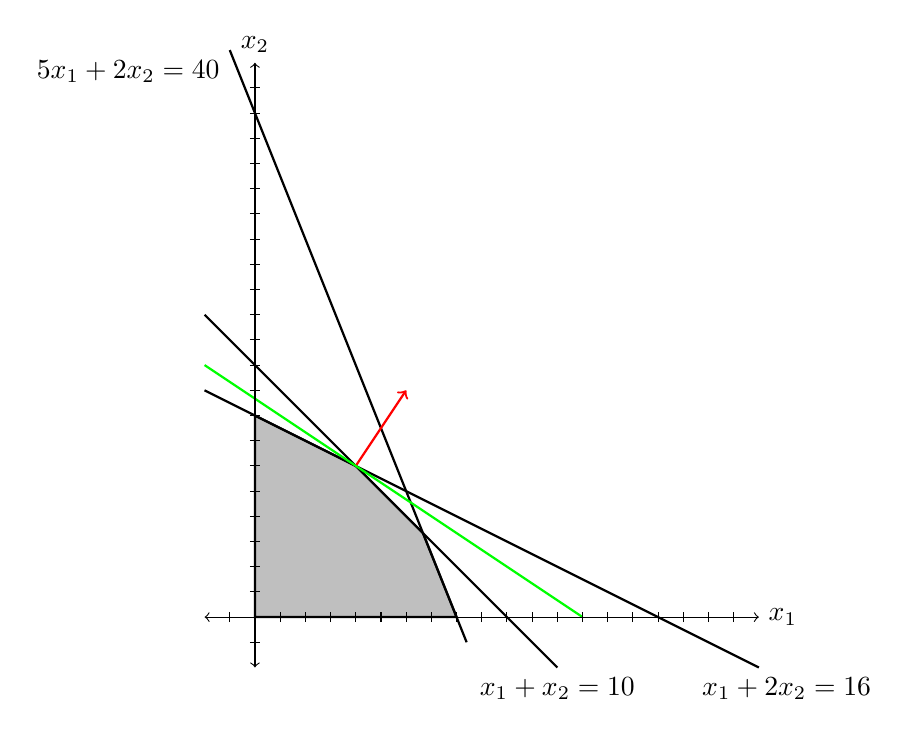
\begin{tikzpicture}[scale=0.32]
    \coordinate (a) at (0,0);
    \coordinate (b) at (8,0);

    \coordinate (c1x) at (12, -2);
    \coordinate (c1y) at (-2, 12);

%    \coordinate (c1y) at (0,     5);
%    \coordinate (c1x) at (6.666, 0);

    \coordinate (c2y) at (-2,  9);
    \coordinate (c2x) at (20, -2);

    \coordinate (c3y) at (-1,  22.5);
    \coordinate (c3x) at (8.4, -1);

%    \coordinate (x) at (intersection of c1x--c1y and c2x--c2y);

    \coordinate (c) at (intersection of c1x--c1y and c3x--c3y);
    \coordinate (d) at (intersection of c1x--c1y and c2x--c2y);

    \coordinate (e) at (0,8);


    \draw[thick,fill=lightgray] (a) -- (b) -- (c) -- (d) -- (e) --cycle;
    \draw[thick] (c1y) -- (c1x) node[below] {\BLACK{$x_1 + x_2 = 10 $}};  
    \draw[thick] (c2y) -- (c2x) node[below] {\BLACK{$\quad\quad x_1 + 2x_2 = 16  $}};
    \draw[thick] (c3x) -- (c3y) node[below left] {\BLACK{$5x_1 + 2x_2 = 40  $}};
    \draw[thick,red,->] (d) -- +(2,3);
    \draw[thick,green] (d) +(-6,4) -- +(9,-6);


    \draw[<->] (-2,0) -- (20,0) node[right] {$x_1$};
    \draw[<->] (0,-2) -- (0,22) node[above] {$x_2$};

    \foreach \i in {-1,...,19} {
        \draw (\i,-0.2) -- (\i,0.2); 
    }
    \foreach \i in {-1,...,21} {
        \draw (-0.2, \i) -- (0.2, \i);
    }

%    \foreach \i in {1,...,19} {
%       \foreach \j in {1,...,21} {
%         \fill (\i,\j) circle (1.5pt);
%       }
%    }
  \end{tikzpicture}
\end{center}
\caption{\label{fig::ex1} Graphic solution of the first example.}
\end{figure}

\subsection{Optimization Problems}

\linebox{
\definition{
An {\hi optimization problem}{\index{Optimization problem}}
is a pair $(I,f)$ where $I$ is a set
and $f:I \to \R$ is a mapping.
The elements of $I$ are called {\hi feasible solutions} of $(I,f)$.
If $I = \emptyset$, the optimization problem
$(I,f)$ is called {\hi infeasible}, otherwise we call it {\hi feasible}.
The function $f$ is called 
the {\hi objective function} of $(I,f)$.\index{Objective function}

We either ask for an element {$x^* \in I$} such that
for all {$x \in I$} we have {$f(x) \leq f(x^*)$} (then {$(I,f)$} is called a
{\hi maximization problem}){\index{Maximization problem}}
or for an element {$x^* \in I$} such that
for all {$x \in I$} we have {$f(x) \geq f(x^*)$} (then {$(I,f)$} is called a
{\hi minimization problem}).{\index{Minimization problem}}
In both cases, such an element $x^*$ is called an {\hi optimum
solution}. $(I,f)$ is {\hi unbounded}{\index{Unbounded optimization problem}}
 if for all $K \in \R$, there is an 
$x \in I$ with $f(x) > K$ (for the maximization problem) or an
$x \in I$ with $f(x) < K$ (for the minimization problem).
An optimization problem is called 
{\hi bounded}{\index{Bounded optimization problem}} if it is
not unbounded.\\
}
}

In this lecture course, we consider optimization problems with linear 
objective functions and linear constraints. The constraints can be written
in a compact way using matrices:

\problem{Linear Programming}
{A matrix $A \in \R^{m \times n}$, vectors $c \in \R^n$
and $b \in \R^m$.}
{Task:}{Find a vector $x \in \R^n$ with $A x \leq b$ maximizing
$c^t x$.}  \index{Linear Program@{\sc Linear Program}}

{\bf Notation:}
Unless stated differently, always let 
$A= (a_{ij})_{{i=1,\dots,m}\atop{j=1,\dots,n}} \in \R^{m\times n}$,
$b=(b_1,\dots,b_m) \in \R^m$ and $c=(c_1,\dots,c_n) \in \R^n$.


{\bf Remark:} Real vectors are simply ordered sets of real numbers.
%If not stated differently, we index their entries of a vector of length
%$n$ from $1$ to $n$, so for $c \in \R^n$ we write
%$c = (c_1, \dots, c_n)$. 
But when we multiply
vectors with each other or with matrices, we have to interpret them
as $n\times 1$-matrices (column vectors) or as 
$1 \times n$-matrices (row vectors). By default, we consider vectors 
as column vectors
in this context, so if we want to use them as row vectors, we have
to transpose them (``$c^t$'').


We often write linear programs in the following way:
\begin{equation} \label{eq::lp_ineq}
\begin{array}{rcl}
\max c^t x & & \\
 \mbox{s.t. \quad} Ax & \leq & b
\end{array}
\end{equation}


Or, in a shorter version we write: $\max\{c^t x \mid Ax \leq b \}$.

%If $A= (a_{ij})_{{i=1,\dots,m}\atop{j=1,\dots,n}}$ and
%$b = (b_1,\dots,b_n)$, then 
The $i$-th row of
matrix $A$ encodes the constraint
${\sum_{j=1}^n a_{ij} x_j \leq b_i}$ on a solution
$x = (x_1,\dots,x_n)$. We could also allow equation constraints
of the form ${\sum_{j=1}^n a_{ij} x_j = b_i}$ but
(as mentioned in the example in Section~\ref{sec::first_example})
these could be easily replaced by two
inequalities. The formulation (\ref{eq::lp_ineq}) which avoids
such equation constraints is called 
{\hi standard inequality form}.{\index{Standard inequality form}}
Obviously, we can also handle minimization problems with this 
approach because minimizing the objective function $c^t x$ means
maximizing the objective function $-c^t x$.

%Feasible and optimal solutions.


%\begin{center}
%  \begin{tikzpicture}[scale=0.6]
%    \coordinate (a) at (0,0);

%    \coordinate (c1y) at (0,     5);
%    \coordinate (c1x) at (6.666, 0);

%    \coordinate (c2y) at (0,6.666);
%    \coordinate (c2x) at (2.666,0);

%    \coordinate (x) at (intersection of c1x--c1y and c2x--c2y);

%    \draw[->] (0,0) -- (8,0);
%    \draw[->] (0,0) -- (0,8);

%    \draw[thick,fill=gray] (a) -- (c1y) -- (x) -- (c2x) --cycle;
%    \draw[green,thick] (c1x) -- (c1y) node[left] {\GREEN{$3x + 4y = 20000 $}};  
%    \draw[blue,thick] (c2x) -- (c2y) node[left] {\BLUE{$ 1.5x + 0.6y = 4000   $}};
%    \draw[thick,red,->] (x) -- +(1.5,1.5);
%    \draw[dotted,thick,red] (x) +(-1.5,1.5) -- +(1.5,-1.5);
%  \end{tikzpicture}
%\end{center}

A second important standard form for linear programs is the 
{\hi standard equation form}: {\index{Standard equation form}}
\begin{equation} \label{eq::lp_eq}
\begin{array}{rcl}
 \max c^t x & & \\
 \mbox{s.t. \quad} Ax & = & b\\
 x & \geq & 0
\end{array}
\end{equation}


Both standard forms can be transformed into each other:
If we are given a linear program in standard equation form we can 
replace each equation by a pair of inequalities and 
the constraint $x\geq 0$ by $-I_n x \leq 0$ (where $I_n$ is always 
the $n\times n$-identity matrix).
This leads to a formulation of the same linear program in standard 
inequality form.

The transformation from the standard inequality form into the
standard equation form is slightly more complicated:
Assume we are given the following linear program in standard
inequality form
\begin{equation}
\begin{array}{rcl}\label{eq::std1}
\max c^t x & & \\
 \mbox{s.t. \quad} Ax & \leq & b
\end{array}
\end{equation}
We replace each variable $x_i$ by two variables $z_i$ and
$\bar z_i$. Moreover, for each of the $m$ constraints we introduce
a new variable $\tilde x_i$
(a so-called {\hi slack variable}{\index{Slack variable}}).
With variables $z=(z_1,\dots,z_n)$, $\bar z=(\bar z_1,\dots,\bar z_n)$ and
$\tilde x = (\tilde x_1,\dots,\tilde x_m)$, we state the following LP
in standard equation form:
\begin{equation}
\begin{array}{rcl}\label{eq::std2}
\max c^t (z - \bar z) & & \\
 \mbox{s.t. \quad} [A\,|\, -A\,|\, I_m] 
   \left( \begin{array}{c}
             z\\
           \bar z\\
          \tilde x
       \end{array}  \right) & = & b\\
    z, \bar z,\tilde x & \geq & 0\\
\end{array}
\end{equation}
Note that $[A \,|\, -A \,|\, I_m]$ is the $m \times {2n+m}$-matrix
that we get by concatenating the matrices $A$, $-A$ and $I_m$.
Any solution $z$,$\bar z$ and $\tilde x$ of the LP~(\ref{eq::std2})
gives a solution of the LP~(\ref{eq::std1}) with the same cost 
by setting: $x_j := z_j - \bar z_j$ (for $j \in \{1,\dots,n\}$).

On the other hand, if $x$ is a solution of LP~(\ref{eq::std1}),
then we get a solution of  LP~(\ref{eq::std2}) with the same cost
by 
setting $z_j := \max\{x_j,0\}$, $\bar z_j := -\min\{x_j,0\}$
(for $j \in \{1,\dots,n\}$) and $\tilde x_i = b_i - \sum_{j=1}^n a_{ij} x_j$
(for $i \in \{1,\dots,m\}$, where $\sum_{j=1}^n a_{ij} x_j \leq b_i$
is the $i$-th constraint of $Ax \leq b$).

Note that (in contrast to the first transformation)
this second transformation (from the standard inequality form
into the standard equation form)
leads to a different solution
space because we have to introduce new variables.

%If we are given a linear program in 
%standard inequality form, we can transform the inequalities to
%equations by adding
%so-called {\hi slack variables}{\index{Slack variable}}: A constraint
%$a_j \cdot x \leq b_j$ can be replaced equivalently by the 
%constraints $a_j ^t x +\tilde x_j = b_j$ and
%$\tilde x_j \geq 0$. This means for each constraint we introduce a new
%non-negative slack variable. Moreover, each variable $x_i$ (that can be negative)
%of the initial LP can be replaced equivalently by two variables
%$z_i, \bar z_i$ with the constraints $z_i, \bar z_i \geq 0$. Each
%occurrence of $x_i$ is then replaced by $z_i - \bar z_i$.


%Equivalence of the different forms: Slack variables,{\index{Slack variable}}
%non-negativity constraints on variables



\subsection{Possible Outcomes}

There are three possible outcomes for a linear program
$\max\{c^t x \mid Ax \leq b \}$:

\begin{itemize}
\item The linear program can be {\hi infeasible}.
This means that $\{x \in \R^n \mid Ax \leq b\} = \emptyset$.
A simple example is:
\begin{equation}
\begin{array}{rcl}
\max x & & \\
 \mbox{s.t. \quad} x & \leq & 0\\
                  -x & \leq & -1
\end{array}
\end{equation}
\item The linear program can be {\hi feasible but unbounded}.
This means that for each constant $K$ there is a 
feasible solution $x$ with $c^t x \geq K$. An example is
\begin{equation}
\begin{array}{rcl}
\max x & & \\
 \mbox{s.t. \quad} x - y & \leq & 0\\
                   y - x & \leq & 1
\end{array}
\end{equation}
\item The linear program can be {\hi feasible and bounded},
so there is an $x \in \R^n$ with $Ax \leq b$ and we have
$\sup\{c^t x \mid Ax \leq b \} < \infty$.
An example is the LP that we saw in Section~\ref{sec::first_example}.
It will turn out that in this case there is always a vector
$\tilde x \in \R^n$ with $A \tilde x \leq b$ with
$c^t \tilde x = \sup\{c^t x \mid Ax \leq b \}$.
\end{itemize}

We will see that deciding if a linear program is feasible is as hard
as computing an optimum solution to a feasible and bounded linear
program (see Section~\ref{sec::StrongDuality}).


% \linebox{
% \theorem{
% Assume that $P = \{x \in \R^n \mid Ax\le b\}$
% (for  $A\in \R^{m\times n}$ and $b \in \R^m$)
% is non-empty. Further assume that
% $\delta := \sup \{c^t x \mid Ax \leq b\}$
%  (for $c \in \R^n$) is finite. Then, there is a vector
% $x \in \R^n$ with $Ax\leq b$ such that $c^t x = \delta$.\\
% }
% }

% \prove
% 
% \endproof


\subsection{Integrality Constraints}

In many applications, we need an integral solution.
This leads to the following class of problems: 

%(Mixed) integer linear programs

\problem{Integer Linear Programming}
{A matrix $A \in \R^{m \times n}$, vectors $c \in \R^n$
and $b \in \R^m$.}
{Task:}{Find a vector $x \in \Z^n$ with $A x \leq b$ maximizing
$c^t x$.} \index{Integer Linear Program@{\sc Integer Linear Program}}

Replacing the constraint $x \in \R^n$ by $x \in \Z^n$ makes a huge
difference. We will see that there are polynomial-time algorithms
for {\sc Linear Programming} while {\sc Integer Linear Programming}
is NP-hard.

Of course, one can also consider optimization problems where we have 
integrality constraints only for some of the variables. These
linear optimization problems are called 
{\sc Mixed Integer Linear Programs}. 
\index{Mixed Integer Linear Program@{\sc Mixed Integer Linear Program}}


\subsection{Modeling of Optimization Problems as (Integral) Linear Programs}


We consider some examples how optimization problems can be modeled as 
LPs or ILPs. Many flow problems can easily formulated as linear programs:

\linebox{
\definition{
Let $G$ be a directed graph with capacities $u:E(G)\to \R_{>0}$ and let
$s$ and $t$ be two vertices of $G$. A feasible 
{\hi $s$-$t$-flow}
in $(G,u)$ is a mapping $f:E(G) \to \R_{\geq 0}$ with
\begin{itemize}
\item $f(e) \leq u(e)$ for all $e \in E(G)$ and
\item $\sum_{e \in \delta^+_G(v)} f(e) - \sum_{e \in \delta^-_G(v)} f(e) = 0$ for all $v \in V(G)\setminus\{s,t\}$.
\end{itemize}
The {\hi value} of an $s$-$t$-flow $f$ is 
$\mbox{val}(f) = \sum_{e \in \delta^+_G(s)} f(e) - \sum_{e \in \delta^-_G(s)} f(e)$.\\
{\index{s-t-flow@{$s$-$t$-flow}}}
}
}


\problem{Maximum-Flow Problem}
{A directed Graph $G$, capacities $u: E(G) \to \R_{> 0}$,
vertices $s, t \in V(G)$ with $s \neq t$.}
{Task:}{Find an $s$-$t$-flow $f:E(G) \to \R_{\geq 0}$
of maximum value.
}{\index{Maximum-Flow Problem@{\sc Maximum-Flow Problem}}


This problem can be formulated as a linear program in the following way:


\begin{equation}\label{eq::maximum_flow_lp}
\begin{array}{rrcll}
 \max    &        \sum\limits_{e \in \delta^+_G(s)} x_e - \sum\limits_{e \in \delta^-_G(s)} x_e & &\\
s.t.\quad     & x_e & \geq & 0              & \mbox{for } e \in E(G)\\
              & x_e & \leq & u(e)           &  \mbox{for } e \in E(G)\\
& \sum\limits_{e \in \delta^+_G(v)} x_e - \sum\limits_{e \in \delta^-_G(v)} x_e & = & 0 & 
      \mbox{for } v \in V(G)\setminus\{s,t\}
\end{array}
\end{equation}


It is well known that the value of a maximum $s$-$t$-flow equals
the capacity of a minimum cut separating $s$ from $t$. 
We will see in 
Section~\ref{section::ComplementarySlackness} that this result
also follows from properties of the linear program formulation.
Moreover, if the capacities are integral, there is always a
maximum flow that is integral (see Section~\ref{sec::TU}).
% We will see in 
%Section~\ref{section::ComplementarySlackness} that these results
%also follow from properties of the linear program formulation.


In some cases, we first have to modify a given optimization problem slightly
in order to get a linear program formulation. See the following
example of a modified version of the {\sc Maximum-Flow Problem} where we have
two sources and want to maximize the minimal out-flow of both sources.

\problem{Bottleneck Maximum-Flow Problem with 2 Sources}
{A directed Graph {$G$}, capacities {$u: E(G) \to \R_{> 0}$},\\
three vertices {$s_1, s_2, t \in V(G)$}.}
{Task:}{Find a mapping {$f :E(G) \to \R_{\geq 0}$} with
\begin{itemize}
\item {$f(e) \leq u(e)$} for all {$e \in E(G)$} and
\item {$\Delta_f(e) = 0$} for all {$v \in V(G) \setminus\{s_1,s_2,t\}$}
\end{itemize} such
that {$\min\{\Delta_f(s_1), \Delta_f(s_2)\}$} is maximized

}

The objective function here is not a linear function but the
minimum of two linear function.
To see how such a problem can be written as an LP, we 
assume slightly more general
that we are given the following optimization problem:


\[
\begin{array}{rc}
 \max &  \min\{c^t x + d, e^t x + f\}   \\
 \mbox{s.t.} & Ax \leq  b\\
\end{array}
\]
for some $c,e \in \R^n$ and $d,f \in \R$. 

This is not a linear program because the objective function 
is not a linear function but a piecewise linear function.
Though the objective function ist not linear,
we can define an equivalent linear program in the following way:
\[
\begin{array}{rrcl}
 \max &  \sigma  \\
  \mbox{s.t.} & \sigma - c^tx & \leq & d \\
              & \sigma - e^tx & \leq & f \\
              & Ax & \leq & b\\
\end{array}
\]


And of course, this trick also works if we want to compute the minimum of
more than two linear functions.

More or less the same trick can be applied to the following problem
in which the
objective function contains absolute values of linear functions:

\[
\begin{array}{rc}
 \min &  |c^t x + d| \\
 \mbox{s.t.} & Ax \leq  b\\
\end{array}
\]
for some $c \in \R^n$ and $d \in \R$. 
Again the problem can
be written equivalently as a linear program in the following form:
\[
\begin{array}{rrcl}
 \max &  -\sigma \\
 \mbox{s.t.}  & -\sigma - c^t x & \leq & d\\
              & -\sigma + c^t x & \leq & -d\\
              & Ax & \leq & b\\
\end{array}
\]
The two additional constraints on $\sigma$ ensure that
we have $\sigma \geq \max\{c^t x + d, -c^t x - d\} = |c^t x + d|$.


Other problems allow a formulation as an ILP but assumably not
an LP formulation:


\problem{Vertex Cover Problem}
{An undirected graph $G$, weights $c: V(G) \to \R_{\geq 0}$.}
{Task:}{Find a set $X \subseteq V(G)$ with $\{v,w\} \cap X \neq \emptyset$
for all $e=\{v,w\} \in E(G)$ such that
$\sum_{v \in X} c(v)$ is minimized.
}{\index{Vertex Cover Problem@{\sc Vertex Cover Problem}}

This problem is known to be NP-hard (see standard textbooks 
like \cite{KorV18}), 
so we cannot hope for a polynomial-time algorithm.
Nevertheless, the problem can easily be formulated as an integer linear program:
\begin{equation}\label{eq::vertex_cover_ilp}
\begin{array}{rll}
           & \min \sum_{v \in V(G)} x_v c(v) & \\
s.t.\quad  & x_v + x_w \geq 1             & \text{for } \{v,w\} \in E(G)\\
           & x_v \in \{0,1\}              & \text{for } v \in V(G)
\end{array}
\end{equation}
For each vertex $v \in V(G)$, we have a $0$-$1$-variable
$x_v$ which is 1 if and only if $v$ should be in the set $X$, i.e.\ if
$(x_v)_{v \in V(G)}$ is an optimum solution to
(\ref{eq::vertex_cover_ilp}), the set $X=\{v \in V(G) \mid x_v = 1\}$
is an optimum solution to the {\sc Vertex Cover Problem}.

This example shows that {\sc Integer Linear Programming} itself is an NP-hard problem.
By skipping the integrality constraints ($x_v \in \{0,1\}$)
 we get the following linear program:
\begin{equation}\label{eq::vertex_cover_lp}
\begin{array}{rll}
           & \min \sum_{v \in V(G)} x_v c(v) & \\
s.t.\quad  & x_v + x_w \geq 1             & \text{for } \{v,w\} \in E(G)\\
           & x_v       \geq 0             & \text{for } v \in V(G)\\
           & x_v       \leq 1             & \text{for } v \in V(G)\\
\end{array}
\end{equation}
We call this linear program an {\hi LP-relaxation}{\index{LP-relaxation}}
of (\ref{eq::vertex_cover_ilp}). 
In this particular case, the relaxation gives a 2-approximation 
of the {\sc Vertex Cover Problem}: For any
solution $x$ of the relaxed problem, we get an integral solution $\tilde x$
by setting 
\[
   \tilde x_v = \left\{ \begin{array}{rcl}
                     1 & : & x_v \geq \frac{1}{2}\\
                     0 & : & x_v  < \frac{1}{2}\\
                      \end{array}
                \right. 
\]
It is easy to check that yields a feasible solution of the ILP
with $\sum\limits_{v \in V(G)} \tilde x_v c(v) \leq 2 \sum\limits_{v \in V(G)} x_v c(v)$.


Obviously, in minimization problems
relaxing some constraints can only decrease the value of
an optimum solution. We call the supremum of the ratio between
the values of the optimum solutions of an ILP and 
its LP-relaxation the {\hi integrality gap}{\index{Integrality Gap}}
of the relaxation. The rounding procedure described above also proves
that in this case the integrality gap is at most $2$. Indeed, $2$ {\em is} 
the integrality gap as the example of a complete graph with 
weights $c(v) = 1$ for all vertices $v$ shows.
For the {\sc Maximum-Flow Problem} with integral edge capacities, the
integrality gap is 1 because there is always an optimum flow that is
integral.


%Vertex cover: 2-approximation by rounding LP solution

%Stable set

The following problem is NP-hard as well:

\problem{Stable Set Problem}
{An undirected graph $G$, weights $c: V(G) \to \R_{\geq 0}$.}
{Task:}{Find a set $X \subseteq V(G)$ with $|\{v,w\} \cap X| \leq 1$
for all $e=\{v,w\} \in E(G)$ such that
$\sum_{v \in X} c(v)$ is maximized.
}{\index{Stable Set Problem@{\sc Stable Set Problem}}


Again, this problem can easily be formulated as an integer linear program:
\begin{equation}\label{eq::stable_set_ilp}
\begin{array}{rll}
           & \max \sum_{v \in V(G)} x_v c(v) & \\
s.t.\quad  & x_v + x_w \leq 1             & \text{for } \{v,w\} \in E(G)\\
           & x_v \in \{0,1\}              & \text{for } v \in V(G)
\end{array}
\end{equation}

An LP-relaxation looks like this:

\begin{equation}\label{eq::stable_set_lp}
\begin{array}{rll}
           & \max \sum_{v \in V(G)} x_v c(v) & \\
s.t.\quad  & x_v + x_w \leq 1             & \text{for } \{v,w\} \in E(G)\\
           & x_v       \geq 0             & \text{for } v \in V(G)\\
           & x_v       \leq 1             & \text{for } v \in V(G)\\
\end{array}
\end{equation}


Unfortunately, in this case, the LP-relaxation is of no use.
Even if $G$ is a complete graph (were a feasible solution of the 
{\sc Stable Set Problem} can contain at most one vertex), setting
$x_v=\frac{1}{2}$ for all $v \in V(G)$ would be a feasible solution
of the LP-relaxation. This example shows that the integrality gap 
is at least $\frac{n}{2}$.
Hence, this LP-relaxation does not provide any
useful information about a good ILP solution.



%%%%%%%%%%%%%%%%%%%%%%%%%%%
\subsection{Polyhedra}
%%%%%%%%%%%%%%%%%%%%%%%%%%%

In this section, we examine basic properties of solution spaces
of linear programs.



\linebox{
\definition{
Let $X \subseteq \R^n$ (for $n \in \N$).
$X$ is called {\hi convex}{\index{Convex}} if 
for all $x,y \in X$ and $t \in [0,1]$ we have $t x +  (1-t) y \in X$.\\
}}


\linebox{
\definition{
For $x_1,\dots,x_k \in \R^n$, $\lambda_1,\dots,\lambda_k$, 
$\lambda_i \geq 0$ ($i \in \{1,\dots,k\}$) with 
$\sum_{i=1}^k \lambda_i = 1$, we call $x = \sum_{i=1}^k \lambda_i x_i$
{\hi convex combination}{\index{Convex combination}} 
of $x_1,\dots,x_k$.
The {\hi convex hull}{\index{Convex hull}} $\mbox{conv}(X)$
of a set $X \subseteq \R^n$ is the set of 
all convex combinations of sets of vectors in $X$.\\
}
}

{\bf Remark:} It is easy to check that the convex hull of a set 
$X \subseteq \R^n$ is the (inclusion-wise) minimal convex set
containing $X$.

\linebox{
\definition{
Let $X\subseteq \R^n$ for some $n \in \N$.
\begin{itemize}
\item[(a)] $X$ is called a {\hi half-space}{\index{Half-space}} if there is 
  a vector $a \in \R^n\setminus\{0\}$ and a number $b\in \R$
  such that $X=\{x \in \R^n \mid a^t x \leq b\}$.
  The vector $a$ is called a {\hi normal}{\index{Normal}} of $X$.
\item[(b)] $X$ is called a {\hi hyperplane}{\index{Hyperplane}} if there is 
  a vector $a \in \R^n\setminus\{0\}$ and a number $b \in \R$
  such that $X=\{x \in \R^n \mid a^t x = b\}$.
  The vector $a$ is called a {\hi normal} of $X$.
\item[(c)] $X$ is called a {\hi polyhedron}{\index{Polyhedron}} if  
  there are a matrix $A \in \R^{m \times n}$ and a vector $b \in \R^m$ such that
  $X = \{x \in \R^n \mid A x \leq b \}$.
\item[(d)] $X$ is called a {\hi polytope}{\index{Polytope}}
if it is a polyhedron and there is a number $K \in \R$
  such that $||x|| \leq K$ for all $x \in X$.
\end{itemize}
}}


{\bf Examples:} The empty set is a polyhedron because 
$\emptyset = \{ x \in \R^n \mid \zero^t x \leq -1 \}$
%(where $\zero$ is the all-zero vector)
and, of course, it is a polytope.
$\R^n$ is also a polyhedron, because 
$\R^n = \{ x \in \R^n \mid \zero^t x \leq 0 \}$
(but, of course, $\R^n$ is not a polytope).

{\bf Observation:} Polyhedra are convex and closed (see exercises).

\linebox{
\lemma{
A set $X \subseteq \R^n$ is a polyhedron if and only if one of the
following conditions holds:
\begin{itemize}
   \item $X = \R^n$
   \item $X$ is the intersection of a finite number of half-spaces.
\end{itemize}
}}

\prove
``$\Leftarrow$:''
If $X = \R^n$ or $X$ is the intersection of a finite number of half-spaces,
it is obviously a polyhedron.

``$\Rightarrow$:''
Assume that $X$ is a polyhedron but $X\neq \R^n$. 
If $X = \emptyset$, then 
$X = \{ x \in \R^n \mid \one_n^t x \leq -1 \} \cap 
     \{ x \in \R^n \mid - \one_n^t x \leq -1 \}$
(where $\one_n$ is the all-one vector of length $n$).
Hence we can assume that $X \neq \emptyset$.

Let $A \in \R^{m \times n}$ be a matrix and $b \in \R^m$ a vector 
with  $X = \{x \in \R^n \mid A x \leq b \}$.
Denote the rows of $A$ by $a_1,\dots a_m$. 
If $a_j = \zero$ for an $j \in \{1,\dots,m\}$, then $\b_j \geq 0$ (where 
$b=(\b_1,\dots,\b_m)$)
because otherwise $X = \emptyset$. Hence we have
\[
   X = \bigcap_{j=1}^m \{x \in \R^n \mid a_j^t x \leq \b_j\} 
     = \bigcap_{j=1,\dots,m:a_j \neq 0} \{x \in \R^n \mid a_j^t x \leq \b_j\},
\]
which is a representation of $X$ as an intersection of a finite number
of half-spaces.
\endproof

\paragraph{Affine combinations and dimension}
If we remove the nonnegativity of the $\lambda_i$'s in the definition of convex combinations, we get the concept of \emph{affine combinations}:

\linebox{
\definition{
For $x_1,\dots,x_k \in \R^n$, $\lambda_1,\dots,\lambda_k\in\R$  with 
$\sum_{i=1}^k \lambda_i = 1$, we call $x = \sum_{i=1}^k \lambda_i x_i$
{\hi affine combination}{\index{affine combination}} 
of $x_1,\dots,x_k$.
The {\hi affine hull}{\index{affine hull}} $\mbox{aff}(X)$
of a set $X \subseteq \R^n$ is the set of 
all affine combinations of sets of vectors in $X$.
The vectors $x_1,\dots,x_k \in \R^n$ are \emph{affinely independent}, if none of them can be written as an affine combination of the other vectors.\\
}
}

A set of vectors is \emph{affinely dependent} if they are not affine independent.
We can characterize affine independence as follows:

\linebox{
\lemma{
The vectors $x_1,\ldots,x_k\in \R^n$ are affinely independent if and only if $\lambda_1=\lambda_2=\ldots=\lambda_k=0$ is the unique solution to the system 
\begin{equation}\label{eq:affine-dep}
    \begin{aligned}
     \sum_{i=1}^k \lambda_i x_i&=0\, \\
 \sum_{i=1}^k \lambda_i &=0 \, .
    \end{aligned}
\end{equation}
}}
\prove
We show the equivalent statement that  $x_1,\ldots,x_k\in \R^n$ are affinely dependent if and only if the  system \eqref{eq:affine-dep} has a nonzero (i.e., not identically zero) solution. 

``$\Leftarrow$:'' Assume $x_1,\ldots,x_k\in \R^n$ are affine dependent. Without loss of generality, assume the first one, $x_1$, can be written as an affine combination of the others, i.e., $x_1=\sum_{i=2}^k \mu_i x_i$ for coefficients $\mu_2,\ldots,\mu_k\in\R$, $\sum_{i=2}^k \mu_i=1$. Then, $\lambda_1=1$, $\lambda_i=-\mu_i$, for $i=2,\ldots,k$ gives a nonzero solution to \eqref{eq:affine-dep}.

``$\Rightarrow$:'' Assume \eqref{eq:affine-dep} has a nonzero solution $\lambda_1,\ldots,\lambda_k$. Without loss of generality, assume $\lambda_1\neq 0$. Then, we can express $x_1$ as the affine combination $x_1=\sum_{i=2}^k \mu_i x_i$,  $\sum_{i=2}^k \mu_i=1$ using the coefficients $\mu_i=-\lambda_i/\lambda_1$ for $i=2,\ldots,k$.
\endproof

{\bf Observation:} The vectors $x_1,\dots,x_k\in\R^n$ are affinely independent if and only if  $x_2-x_1$, $x_3 - x_1, \dots, x_k - x_1$
are linearly independent. 


\linebox{
\definition{
The {\hi dimension}{\index{Dimension}} of a set $X \subseteq \R^n$, denoted as $\dim(X)$, is the largest number of affinely independent vectors in $X$ minus 1.\\
}}


Thus, $\dim(\emptyset)=-1$, and $\dim(\R^n)=n$. In class, we also show the following equivalent definition of the dimension.


%{\bf Observation:} The dimension of a set $X \subseteq \R^n$ is the largest $d$ for which $X$ contains elements $v_0,v_1,\dots,v_d$ such that $v_1 - v_0$, $v_2 - v_0, \dots, v_d - v_0$ are linearly independent. 

\linebox{
\lemma{
The {\hi dimension}{\index{Dimension}} of a nonempty set $X \subseteq \R^n$, $X\neq\emptyset$ is
\[
 \dim(X) = n - \max\{\mbox{\em rank}(A) \mid A \in \R^{n \times n} \mbox{ with } Ax=Ay \mbox{ for all }x,y \in X\}.
\]
}}

%In other words, the dimension of $X \subseteq \R^n$ is $n$ minus the maximum size of a set of linear independent vectors that are orthogonal to any difference of elements in $X$. For example, the empty set and sets consisting of exactly one vector have  dimension $0$. The set $\R^n$ has dimension $n$.

 

%To see this, observe that $d$ is obviously a lower bound
%on $ \dim(X)$. On the other hand, any set $v_1 - v_0$, $v_2 - v_0, \dots, v_d - v_0$ of 
%linear independent vectors can be extended to a basis of $\R^n$




\paragraph{Cones}

~~

\linebox{
\definition{
A set $X \subseteq \R^n$
is called a {\hi convex cone}{\index{Convex cone}} if $X\neq\emptyset$ and
for all $x,y \in X$ and 
$\lambda, \mu \in \R_{\geq 0}$ we have $\lambda x + \mu y \in X$.\\
}}

{\bf Observation:} A non-empty set
$X \subseteq \R^n$ is a convex cone if and only
if $X$ is convex and for all $x\in X$ and $\lambda \in \R_{\geq 0}$ we have $\lambda x \in X$.


\linebox{
\definition{
A set $X \subseteq \R^n$ is called a {\hi polyhedral cone}{\index{Polyhedral cone}}
if it is a polyhedron and a convex cone.\\
}
}


\linebox{
\lemma{
A set $X \subseteq \R^n$ is a polyhedral cone if and only if
there is a matrix $A\in\R^{m\times n}$ such that 
$X = \{x \in \R^n \mid  Ax\leq 0\}$.\\
}
}

\prove
``$\Leftarrow$:'' Let $X = \{x \in \R^n \mid  Ax \leq 0\}$
for some matrix $A\in\R^{m\times n}$. Then $X$ obviously is a polyhedron and
non-empty (because $0 \in X$). And if  $x,y \in X$ and 
$\lambda, \mu \in \R_{\geq 0}$, then $A( \lambda x +  \mu y) \leq 0$,
so $\lambda x + \mu y \in X$. Hence $X$ is a convex cone, too.

``$\Rightarrow$:'' Let $X \subseteq \R^n$ be a polyhedral cone.
In particular, there is a matrix $A\in\R^{m\times n}$ and a vector
$b \in \R^m$ such that $X = \{x \in \R^n \mid  Ax \leq b\}$.
Since $X$ is a convex cone, it is non-empty and it must contain
$0$. Therefore, no entry of $b$ can be negative. Thus,
$X \supseteq \{x \in \R^n \mid  Ax \leq 0\}$. But if there was
a vector $x \in X$ such that $Ax$ has positive $i$-th entry 
(for an $i \in \{1,\dots,m\}$), then for sufficiently large
$\lambda$, the $i$-th entry of $\lambda Ax$ would be greater than 
$b_i$ which is a contradiction to the assumption that $X$ is
a convex cone. Therefore, $X = \{x \in \R^n \mid  Ax \leq 0\}$.
\endproof


Let $x_1,\dots,x_m \in \R^n$ be vectors. The cone {\hi generated} by 
$x_1,\dots,x_m$ is the set
\[
\mbox{cone}(\{x_1,\dots,x_m\}) 
:= \left\{\sum_{i=1}^m\lambda_i x_i \mid \lambda_1,\dots,\lambda_m\geq 0\right\}.
\]
A convex cone $C$ is called {\hi finitely generated}{\index{Finitely generated cone}}
if there are 
vectors $x_1,\dots,x_m \in \R^n$ with $C = \mbox{cone}(\{x_1,\dots,x_m\})$.

It is easy to check that $\mbox{cone}(\{x_1,\dots,x_m\})$ is indeed a convex cone.
We will see in Section~\ref{sec::cones} that a cone is polyhedral if and only
if it is finitely generated.


%%%%%%%%%%%%%%%%%%%%%%%%%%%
\section{Duality}
%%%%%%%%%%%%%%%%%%%%%%%%%%%

\subsection{Dual LPs}

%See \cite{MatG07}


%Dual LP: Example as in \cite{MatG07}; weak duality

Consider the following linear program (P):
\[
\begin{array}{rrrrrr}
\max              & 12x_1 & + & 10x_2 &      &\\
\mbox{s.t.}       & 4x_1  & + &  2x_2 & \leq & 5\\
                  & 8x_1  & + & 12x_2 & \leq & 7\\
                  & 2x_1  & - &  3x_2 & \leq & 1
\end{array}
\]
How can we find upper bounds on the value of an optimum solution?
By combining the first two constraints we can get the following bound for
any feasible solution $(x_1,x_2)$:
\[
12x_1 + 10x_2 = 2 \cdot (4x_1+2x_2) + \frac{1}{2}(8x_1+12x_2) \leq 2 \cdot 5 + \frac{1}{2} \cdot 7 = 13.5.
\]
We can even do better by combining the last two inequalities:
\[
12x_1 + 10x_2 = \frac{7}{6} \cdot (8x_1 + 12x_2) + \frac{4}{3} \cdot (2x_1 - 3x_2) \leq \frac{7}{6} \cdot 7 + \frac{4}{3} \cdot 1 = 9.5.
\]
More generally, for computing upper bounds we ask for non-negative numbers $u_1,u_2,u_3$ such that
\[
12x_1 + 10x_2 = u_1 \cdot (4x_1 + 2x_2) + u_2 \cdot (8x_1 + 12x_2) + u_3  \cdot (2x_1 - 3x_2).
\]
Then, $5 \cdot u_1 + 7 \cdot u_2 + 1 \cdot u_3$ is an upper bound on the
value of any solution of (P), so we want to chose $u_1,u_2,u_3$ in such a way that
$5 \cdot u_1 + 7 \cdot u_2 + 1 \cdot u_3$ is minimized.

This leads us to the following linear program (D):
\[
\begin{array}{rrrrrrrr}
\min         & 5 u_1 & + &  7 u_2 & + &   u_3 &\\
\mbox{s.t.}  & 4 u_1 & + &  8 u_2 & + & 2 u_3 & = & 12\\
             & 2 u_1 & + & 12 u_2 & - & 3 u_3 & = & 10\\
             &   u_1 &   &        &    &       & \geq & 0\\
             &       &   &    u_2 &    &       & \geq & 0\\
             &       &   &        &    &  u_3  & \geq & 0
\end{array}
\]
This linear program is called the {\hi dual linear program of (P)}{\index{Dual LP}.
Any solution of (D) yields an upper bound on the optimum value of 
of (P), and in this particular case
it turns out that $u_1 = 0$ , $u_2 = \frac{7}{6}$, $u_3 = \frac{4}{3}$ 
(the second solution from above) with value $9.5$ is an optimum solution of
(D) because
$x_1 = \frac{11}{16}$, $x_2 = \frac{1}{8}$ is a solution of (P) with value $9.5$.

For a general linear program (P)
\begin{eqnarray*}
\max c^t x & & \\
 \mbox{s.t. \quad} Ax & \leq & b
\end{eqnarray*}
in standard inequality form we define its dual linear program (D) as
\begin{eqnarray*}
\min b^t y & & \\
 \mbox{s.t. \quad} A^t y & = & c\\
                   y     & \geq & 0
\end{eqnarray*}

In this context, we call the linear program (P) {\hi primal linear program}.
{\index{Primal LP}}

{\bf Remark:}
Note that the dual linear program does not only depend on the objective
function and the solution space of the primal linear program but on its 
description by linear inequalities. For example adding redundant inequalities
to the system $Ax \leq b$ will lead to more variables in the dual
linear program.


\linebox{
\proposition{
(Weak duality){\index{Weak duality}}
If both the equation systems $Ax \leq b$ and $A^t y = c, y \geq 0$
have a feasible solution, then
\[
   \max\{c^t x \mid Ax\leq b  \} \leq \min\{b^t y \mid A^t y = c, y \geq 0\}.
\]
}}

\prove
For $x$ with $Ax \leq b$ and $y$ with $A^t y = c, y \geq 0$, we have
\[
   c^t x = (A^t y)^t x = y^t Ax \leq y^tb.
\]
\endproof




{\bf Remark:} The term ``dual'' implies that applying the transformation
from (P) to (D) twice yields (P) again. This is not exactly the case
but it is not very difficult to see that dualizing (D) (after transforming
it into standard equational form) gives a linear program that is equivalent
to (P) (see the exercises).




\subsection{Fourier-Motzkin Elimination}

Consider the following system of inequalities:
\begin{equation}\label{eq::FM1}
\begin{array}{rrrrrrr}
3x  & + & 2y & + & 4z & \leq & 10\\
3x  &   &    & + & 2z & \leq & 9\\
2x  & - &  y &   &    & \leq & 5\\
-x  & + & 2y & - &  z & \leq & 3\\
-2x &   &    &   &    & \leq & 4\\
    &   & 2y & + & 2z & \leq & 7
\end{array}
\end{equation}

Assume that we just want to decide if a feasible solution $x,y,z$ exists. 
The goal is to get rid of the variables one after the other.
To get rid of $x$, we first reformulate the inequalities such that we can
easily see lower and upper bounds for $x$:
\begin{equation}\label{eq::FM2}
\begin{array}{rrrrrrr}
x & \leq & \frac{10}{3} & - & \frac{2}{3}y &  - & \frac{4}{3}z\vspace*{1mm}\\
x & \leq &            3 &   &              &  - & \frac{2}{3}z\vspace*{1mm}\\
x & \leq & \frac{5}{2}  & + & \frac{1}{2}y &    &             \vspace*{1mm}\\
x & \geq &           -3 & + &           2y &  - &            z\vspace*{1mm}\\
x & \geq &           -2 &   &              &    &             \vspace*{1mm}\\
    &   & 2y & + & 2z & \leq & 7
\end{array}
\end{equation}

This system of inequalities has a feasible solution if and only if the following 
system (that does not contain $x$) has a solution:
\begin{equation}\label{eq::FM3}
\begin{array}{rcl}
\min\left\{\frac{10}{3} - \frac{2}{3}y  - \frac{4}{3}z, \quad
      3 - \frac{2}{3}z, \quad
      \frac{5}{2}  + \frac{1}{2}y
    \right\} 
& \geq & 
\max\left\{-3 + 2y - z, \quad
      -2   \right\}\\
2y + 2z & \leq & 7
\end{array}
\end{equation}\label{eq::FM4}
This system can be rewritten equivalently in the following way:
\begin{equation}
\begin{array}{rrrrrrrrrrr}
\frac{10}{3} & - & \frac{2}{3}y  & - & \frac{4}{3}z & \geq & -3 & + & 2y & - & z \vspace*{1mm} \\ 
\frac{10}{3} & - & \frac{2}{3}y  & - & \frac{4}{3}z & \geq & -2 &   &    &   &   \vspace*{1mm}\\
       3     &   &               & - & \frac{2}{3}z & \geq &  -3 & + & 2y & - & z \vspace*{1mm}\\
       3     &   &               & - & \frac{2}{3}z & \geq & -2 &   &    &   &   \vspace*{1mm}\\
\frac{5}{2}  & + & \frac{1}{2}y  &   &              & \geq &  -3 & + & 2y & - & z \vspace*{1mm}\\
\frac{5}{2}  & + & \frac{1}{2}y  &   &              & \geq & -2 &   &    &   &   \vspace*{1mm}\\
&   & 2y & + & 2z & \leq & 7
\end{array}
\end{equation}
This is equivalent to the following system in standard form:
\begin{equation}\label{eq::FM5}
\begin{array}{rrrrr}
\frac{8}{3}y  & + & \frac{1}{3}z & \leq & \frac{19}{3}\vspace*{1mm}\\
\frac{2}{3}y  & + & \frac{4}{3}z & \leq & \frac{16}{3}\vspace*{1mm}\\
2y            & - & \frac{1}{3}z & \leq & 6 \vspace*{1mm}\\
              &   & \frac{2}{3}z & \leq & 5 \vspace*{1mm}\\
\frac{3}{2}y  & - &            z & \leq & \frac{11}{2} \vspace*{1mm}\\
-\frac{1}{2}y &   &              & \leq & \frac{9}{2} \vspace*{1mm}\\
2y            & + &           2z & \leq & 7 
\end{array}
\end{equation}
We can iterate this step until we end up with a system of inequalities without
variables. It is easy to check if all inequalities in this final system are
valid, which is equivalent to the existence of a feasible solution of the
initial system of inequalities. Moreover, we can also find a feasible solution if
one exists. To see this, note that any solution of the system~(\ref{eq::FM3})
(that contains $y$ and $z$ as variables only) also gives a solution
of the system~(\ref{eq::FM2}) by setting $x$ to a value in the interval
\[
\left[
\max\left\{-3 + 2y - z, \quad
      -2 \right\}, 
\min\left\{\frac{10}{3} - \frac{2}{3}y  - \frac{4}{3}z, \quad
      3 - \frac{2}{3}z, \quad
      \frac{5}{2}  + \frac{1}{2}y
    \right\}
\right].
\]

Note that this method, 
which is called {\hi Fourier-Motzkin elimination},{\index{Fourier-Motzkin elimination}}
is in general very inefficient. If $m$ is the number of 
inequalities in the initial system, it may be necessary to state $\frac{m^2}{4}$
inequalities in the system with one variable less (this is the case if there
are $\frac{m}{2}$ inequalities that gave an upper bound on the variable
we got rid of and $\frac{m}{2}$ inequalities that gave a lower bound).

Nevertheless, the Fourier-Motzkin elimination
can be used to get a certificate that a given system
of inequalities does {\it not} have a feasible solution. 
In the proof of the following theorem we give a general 
description of one iteration of the method:  

\linebox{
 \theorem{\label{theorem::fouriermotzkin}
Let $A \in \R^{m \times n}$ and $b \in \R^m$ (with $n \geq 1$).
% such that
%$A$ contains at least one non-zero entry.
%Let $Ax \leq b$ be a system of $m$ inequalities with
%. 
Then there are  $\tilde A \in \R^{\tilde m \times (n-1)}$ and  $\tilde b \in \R^{\tilde m}$ 
with $\tilde m \leq m +\frac{m^2}{4}$ such that
\begin{itemize}
%   \item[(a)] The number of columns in $A'$ which contain only zeros is 
%              bigger by at least one than the number of columns in $A$
%              which contain only zeros.
   \item[(a)] Each inequality in the system $\tilde A \tilde x \leq \tilde b$ is a positive
              linear combination of inequalities from $Ax \leq b$
   \item[(b)] 
   The system $Ax \leq b$ has a solution if and only if $\tilde A \tilde x \leq \tilde b$ has a solution. Moreover, for every solution $x=(x_1,x_2,\ldots,x_n)\in\R^{n}$ to $Ax\le b$, $\tilde x=(x_2,\ldots,x_n)\in\R^{n-1}$ is a solution to $\tilde A \tilde x \leq \tilde b$. Conversely, $\tilde x=(x_2,\ldots,x_n)\in\R^{n-1}$ is the solution to the system $\tilde A \tilde x \leq \tilde b$ if and only if there exists an $x_1\in\R$ such that $(x_1,x_2,\ldots,x_n)$ is a solution to  $Ax\le b$.
\end{itemize}
}}

\prove 
Denote the entries of $A$ by $a_{ij}$, i.e.\
$A= (a_{ij})_{{i=1,\dots,m}\atop{j=1,\dots,n}}$. We will show how
to get rid of the variable with index $1$. To this end, we partition
the index set $\{1,\dots,m\}$ of the rows into three disjoint sets
$U$,$L$, and $N$:
\begin{eqnarray*}
  U & := & \{i \in \{1,\dots,m\} \mid a_{i1} > 0\}\\
  L & := & \{i \in \{1,\dots,m\} \mid a_{i1} < 0\}\\
  N & := & \{i \in \{1,\dots,m\} \mid a_{i1} = 0\}\\
\end{eqnarray*}
We can assume that $|a_{i1}| = 1$ for all $i \in U \cup L$
(otherwise we divide the corresponding inequality by $|a_{i1}|$).

For vectors $\bar a_i = (a_{i2},\dots a_{in})$ and $\tilde x = (x_2,\dots x_n)$
(that are empty if $n=1$), we replace the inequalities that correspond
to indices in $U$ and $L$ by
\begin{equation}\label{eq::FMproof1}
\bar a_i^t \tilde x +  \bar a_k^t \tilde x \leq \b_i + \b_k \quad\quad i \in U, k \in L.
\end{equation}
Obviously, each of these $|U|\cdot|L|$ 
new inequalities is simply the sum of two
of the given inequalities (and hence a positive linear combination of them).

The inequalities with index in $N$ 
are rewritten as
\begin{equation} \label{eq::FMproof2}
   \bar a^t_l \tilde x \leq \b_l \quad\quad l \in N.
\end{equation}
The inequalities in (\ref{eq::FMproof1}) and (\ref{eq::FMproof2})
form a set of inequalities $\tilde A \tilde x \leq \tilde b$
with $n-1$ variables, and each solution
of $Ax \leq b$ gives a solution of $\tilde A \tilde x \leq \tilde b$ by restricting
$x=(x_1,\dots,x_n)$ to $(x_2,\dots,x_n)$.

On the other hand, if $\tilde x=(x_2,\dots,x_n)$ is a solution of
$\tilde A \tilde x \leq \tilde b$, then we can
set $\tilde x_1$ to any value in the (non-empty) interval
\[
\left[
\max\{ \tilde a_k^t \tilde x - \b_k  \mid k \in L \}, \quad
\min\{ \b_i - \tilde a_i^t \tilde x  \mid i \in U \}
\right]
\]
where we set the minimum of an empty set to $\infty$ and the maximum of 
an empty set to $-\infty$.
Then, $x = (\tilde x_1, x_2,\dots, x_n)$ is a solution of $Ax\leq b$.
%See \cite{MatG07}

The (non-tight) bound $\tilde m\le m+m^2/4$ follows as $\tilde m=|U|\times |L|+|N|$, where $|U|+|L|+|N|=m$.
 \endproof

{\bf Remark.} In the above proof, if $U=\emptyset$ or $L=\emptyset$, we only keep the inequalities in $N$ for the system $\tilde A\tilde x\le \tilde b$. This is because if $U=\emptyset$, then for any $\tilde x=(x_2,\ldots,x_n)$ satisfying the inequalities in $N$, we can choose a sufficiently large $x_1$ that satisfies all inequalities in $L$. Similarly, if $L=\emptyset$ then we can choose a sufficiently small $x_1$.


\subsection{Farkas' Lemma}


\linebox{
\theorem{(Farkas' Lemma for a system of inequalities)\label{theorem::farkas1}{\index{Farkas' Lemma}}
For $A \in \R^{m \times n}$ and $b \in \R^m$, the
system  $Ax \leq b$ has a solution if and only if there is no vector
$u \in \R^m$ with $u \geq 0$, $u^t A = 0^t$ and $u^t b < 0$.\\
}}


\prove
``$\Rightarrow$:'' If  $Ax \leq b$ and $u \in \R^m$ with
$u \geq 0$, $u^t A = 0^t$ and $u^t b < 0$, 
then $0 = (u^t A) x = u^t (A x) \leq u^t b < 0$, which is a contradiction.\\
``$\Leftarrow$:'' Assume that $Ax \leq b$ does not have a solution.
%We may assume that $A$ does not contain a vector of zeros as a column.
Let $A^{(0)} := A$ and $b^{(0)} := b$. 
We apply Theorem~\ref{theorem::fouriermotzkin}
to $A^{(0)}x^{(0)} \leq b^{(0)}$ and get a system 
$A^{(1)}x^{(1)} \leq b^{(1)}$ of inequalities with $n-1$ variables
%at least one column in  $A^{(2)}$ consisting of zeros 
such that $A^{(1)}x^{(1)} \leq b^{(1)}$
 does not have a solution either and such that each inequality of
$A^{(1)}x^{(1)} \leq b^{(1)}$
is a positive linear combination of inequalities of $A^{(0)}x^{(0)} \leq b^{(0)}$.
We iterate this step $n$ times, and in the end, we get a system of 
inequalities $A^{(n)}x^{(n)} \leq b^{(n)}$ without variables (so $x^{(n)}$ is
in fact a vector of length 0)
that does
not have a solution. Moreover, each inequality in $A^{(n)}x^{(n)} \leq b^{(n)}$ 
is a positive linear combination of inequalities in $Ax \leq b$.
Since $A^{(n)}x^{(n)} \leq b^{(n)}$ does not have a solution, it must contain
an inequality $0 \leq d$ for a constant $d < 0$. This is a positive
linear combination of inequalities in $Ax \leq b$, so there is
a vector $u \in \R^m$ with $u \geq 0$, $u^t A = 0^t$ and $u^t b = d < 0$.
\endproof


\linebox{
\theorem{(Farkas' Lemma, most general case)\label{theorem::farkas2}
For $A \in \R^{m_1 \times n_1}$, $B \in \R^{m_1 \times n_2}$, 
$C \in \R^{m_2 \times n_1}$, $D \in \R^{m_2 \times n_2}$, $a \in \R^{m_1}$
and $b \in \R^{m_2}$ exactly one of the two following systems has a feasible
solution:\\
System 1:
\begin{equation}
\begin{array}{rclcl}
Ax & + & By & \leq & a\\
Cx & + & Dy & =    & b\\
x  &   &    & \geq & 0
\end{array}
\end{equation}
System 2:
\begin{equation}
\begin{array}{rclcl}
u^tA & + & v^tC & \geq & 0^t\\
u^tB & + & v^tD & =    & 0^t\\
u    &   &     & \geq & 0\\
u^ta & + & v^tb  & < & 0
\end{array}
\end{equation}
}}

\prove
%\ifdefined\OnlineVersion{}
%Exercise.
%\else
The first system is equivalent to 
\begin{equation*}
\begin{array}{rclcr}
Ax        & + & By  & \leq & a\\
Cx        & + & Dy  & \leq & b\\
-Cx       & - & Dy  & \leq & -b\\
-I_{n_1} x &   &     & \leq & 0
\end{array}
\end{equation*}
By Theorem~\ref{theorem::farkas1}, this system has a solution if and only if
the following sytem does not have a solution:
\begin{equation*}
\begin{array}{rclclclcl}
u_1^tA & + & u_2^t C & - & u_3^tC & - & u_4^t &  =   & 0^t\\
u_1^tB & + & u_2^t D & - & u_3^tD &   &      &  =   & 0^t\\
u_1^ta & + & u_2^t b & - & u_3^tb &   &     &  <   & 0^t\\
u_1    &   &         &   &       &   &     & \geq & 0\\
       &   & u_2     &   &       &   &     & \geq & 0\\
       &   &         &   & u_3   &   &     & \geq & 0\\
       &   &         &   &       &   & u_4 & \geq & 0
\end{array}
\end{equation*}
Obviously, this system has a solution if and only if the second system of the 
theorem has a solution.
%\fi %onlineversion
\endproof



\linebox{
\corollary{
(Farkas' Lemma, further variants)\label{theorem::farkas3}
For $A \in \R^{m \times n}$ and $b \in \R^m$, the following
statements hold:
\begin{itemize}
\item[(a)] There is a vector $x \in \R^n$ with
$x\geq 0$ and $Ax=b$ if and only if there is no vector
$u \in \R^m$ with $u^t A \geq 0^t$ and $u^t b < 0$.
\item[(b)] There is a vector $x \in \R^n$ with
$Ax=b$ if and only if there is no vector
$u \in \R^m$ with $u^t A = 0^t$ and $u^t b < 0$.
\end{itemize}
}}

\prove
Restrict the statement of Theorem~\ref{theorem::farkas2} to 
the vector $b$ and matrix $C$ (for part (a)) of $D$ 
(for part (b)).\endproof

{\bf Remark:} Statement (a) of Corollary~\ref{theorem::farkas3}
has a nice geometric interpretation. Let $C$ be the cone generated by the
columns of $A$. Then, the vector $b$
is either in $C$ or there is a hyperplane
(given by the normal $u$) that separates $b$ from $C$.

As an example consider 
$A = \left( \begin{array}{cc}
     2 &  3 \\
     1 &  1
\end{array}
  \right)$ and $b_1 =  {5 \choose 2} $ and $b_2  = {1 \choose 3} $
(see Figure~\ref{fig::cone_rep}).
The vector $b_1$ is in the cone generated by the columns of $A$
(because ${5 \choose 2} = {2 \choose 1} + {3 \choose 1}$) while $b_2$
can by separated from the cone by a hyperplane orthogonal to 
$u  = {1 \choose -2} $.


\begin{figure}[htb]
\begin{center}
  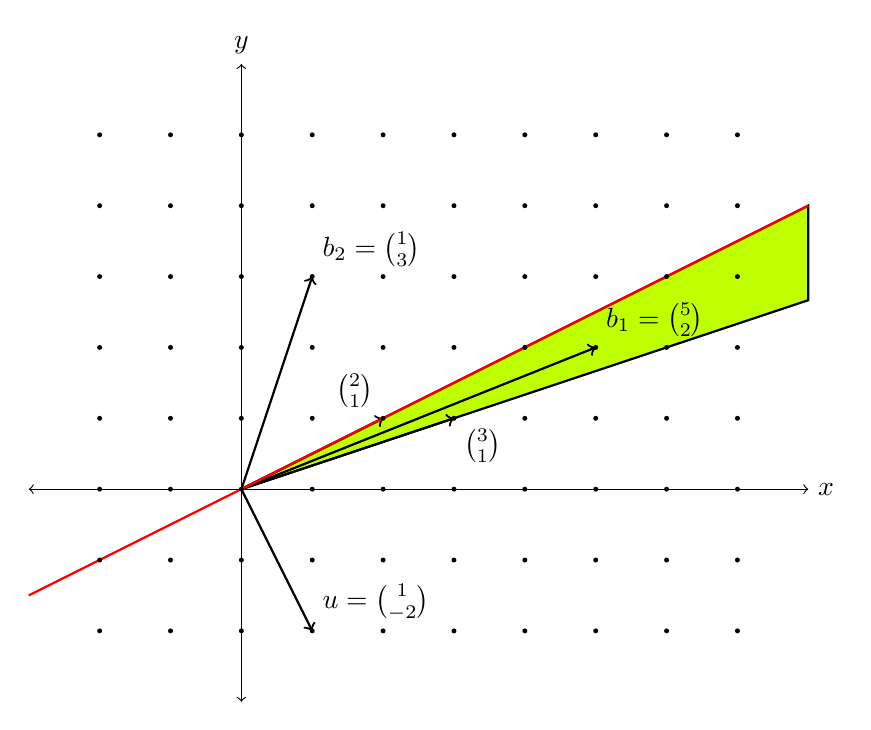
\begin{tikzpicture}[scale=0.9]
    \coordinate (a) at (0,0);

    \coordinate (c1) at (2, 1);
    \coordinate (c2) at (3, 1);

    \coordinate (c1p) at (8, 4);
    \coordinate (c2p) at (8, 2.666666667);

    \coordinate (b1) at (5, 2);
    \coordinate (b2) at (1, 3);

    \coordinate (u) at (1, -2);

    \coordinate (l) at (-3, -1.5);

%    \coordinate (c) at (intersection of c1x--c1y and c3x--c3y);
%    \coordinate (d) at (intersection of c1x--c1y and c2x--c2y);

    \draw[thick,fill={rgb:green,1;yellow,3}] (a) -- (c1p) -- (c2p) --cycle;
    \draw[thick, ->] (a) -- (c1) node[above left] {$2 \choose 1 $};
    \draw[thick, ->] (a) -- (c2) node[below right] {$3 \choose 1 $};
    \draw[thick, ->] (a) -- (b1) node[above right] {$b_1  = {5 \choose 2} $};
    \draw[thick, ->] (a) -- (b2) node[above right] {$b_2  = {1 \choose 3} $};
%    \draw[thick,red,->] (d) -- +(2,3);
%    \draw[thick,green] (d) +(-6,4) -- +(9,-6);

    \draw[thick, ->] (a) -- (u) node[above right] {$u  = {1 \choose -2} $};
    \draw[thick, red] (l) -- (c1p);

    \draw[<->] (-3,0) -- (8,0) node[right] {$x$};
    \draw[<->] (0,-3) -- (0,6) node[above] {$y$};

%    \foreach \i in {-2,...,7} {
%        \draw (\i,-0.1) -- (\i,0.1); 
%    }
%    \foreach \i in {-2,...,5} {
%        \draw (-0.1, \i) -- (0.1, \i);
%    }

    \foreach \i in {-2,...,7} {
       \foreach \j in {-2,...,5} {
         \fill (\i,\j) circle (1.0pt);
       }
    }
  \end{tikzpicture}
\end{center}
\caption{\label{fig::cone_rep}
Example for the statement in Corollary~\ref{theorem::farkas3}(a).}
\end{figure}

Hence, we have get the following corollary.

\linebox{
\corollary{
Let $a_1,\dots,a_n \in \R^m$. Then for any vector $b \in \R^m$ exactly
one of the following statements holds:
\begin{itemize}
   \item[(a)] $b \in \text{cone} (\{ a_1,\dots,a_m\})$.
   \item[(b)] There is a half-space $H$ such that 
      $\{a_1,\dots,a_n\} \subseteq H$ and $b \not\in H$.
\end{itemize}
}
}

\prove
Statement (b) is equivalent to the existence of a vector $u \in \R^m$
with $u^t a_i \geq 0$ for all $i \in \{1,\dots,n\}$ and $u^t b < 0$.
Thus the corollary follows from Corollary~\ref{theorem::farkas3}~(a).
\endproof

\subsection{Strong Duality}\label{sec::StrongDuality}

\linebox{
\theorem{\label{theorem::strong_dual}
(Strong duality)
For the two linear programs
\begin{eqnarray*}
\max c^t x & & \quad\quad(P)\\
 \mbox{s.t. \quad} Ax & \leq & b
\end{eqnarray*}
and 
\begin{eqnarray*}
\min b^t y & &  \quad\quad(D)\\
 \mbox{s.t. \quad} A^t y & = & c\\
                   y     & \geq & 0
\end{eqnarray*}
exactly one of the following statements is true:
\begin{enumerate}
\item Neither (P) nor (D) have a feasible solution.
\item (P) is unbounded and (D) has no feasible solution.
\item (P) has no feasible solution and (D) is unbounded.
\item Both (P) and (D) have a feasible solution. Then
      both have an optimal solution, and for an optimal
      solution $\tilde x$ of (P) and an optimal solution $\tilde y$
      of (D), we have
      \[
         c^t \tilde x = b^t \tilde y.
      \]
\end{enumerate}
}}

\prove
Obviously, at most one of the statements can be true.

If one of the linear programs is unbounded, then the other one must be
infeasible because of the weak duality.

Assume that one of the LPs (say (P) without loss of generality)
is feasible and bounded. The other case, when (D) is feasible and bounded, can be shown with a symmetric argument.
We present two proofs, one using Fourier--Motzkin elimination, and a second one based on Farkas's lemma.


{\em First proof:} 
Note that $\sup \{c^t x\,:\,  Ax\le b\}=\sup\{z\,:\,  z-c^t x\leq 0, Ax\leq b\}$. By the assumption that (P) is feasible and bounded, the supremum is finite.
We apply the Fourier--Motzkin elimination to the system $z-c^t x\leq 0,\, Ax\leq b$, to eliminate the  variables $x_1,\ldots, x_n$. The result is a system $\bar a  z\leq \bar b$ in the single variable $z$, where $\bar a$ and $\bar b$ are vectors. We may assume that the entries of $\bar a$ are $0,\pm1$. By Theorem~\ref{theorem::fouriermotzkin}(b),
$\sup\{z\,:\,  z-c^t x\leq 0, Ax\leq b\}=\sup\{z\,:\,  \bar a z\leq \bar b\}$.
%, and there exists $x^*\in P$ such that $c^t x^*$ achieves the maximum. 
Since $\sup\{z\,:\,  \bar a  z\leq \bar b\}$ is bounded, at least one entry of $\bar a$  equals $1$, and the supremum is taken: 
\[
\sup\{z\,:\,  \bar a  z\leq \bar b\}=\max\{z\,:\, \bar a z\leq \bar b\}=\min_{i\,:\,  \bar a_i=1}\bar b_i\, .\]    
Let $h$ be an index achieving the minimum in the previous equation. By Theorem~\ref{theorem::fouriermotzkin}(a), inequality $ z\leq \bar b_h$ is a nonnegative combination of the $m+1$ inequalities $z-c^t x\leq 0,\, Ax\leq b$. Thus there exists a nonnegative vector $(u_0,u^*)\in\R_{\ge0}\times \R_{\ge0}^m$ such that $u_0=1$, $(u_0,u^*)^t {-c\choose A}=0$ and $({u^*})^t b=\bar b_h$. It follows that $u^*$ is feasible to (D) and ${u^*}^t b=\max\{c^t x\,:\,  x\in P\}$.

{\em Second proof:}
%Assume that (P) has an optimum solution $\tilde x$. 
%We define 
%$\delta := c^t \tilde x$. 
By the assumption that (P) is feasible and bounded,
\begin{equation}\label{eq::proof_dual_1}
\begin{array}{rcl}
Ax & \leq & b\\
%-c^tx & \leq & -\delta
\end{array}
\end{equation}
has a feasible solution, while there is a $B$ such that
the system
\begin{equation}\label{eq::proof_dual_2}
\begin{array}{rcl}
Ax & \leq & b\\
-c^tx & \leq & -B
\end{array}
\end{equation}
does not have a feasible solution.
By Farkas' Lemma (Theorem~\ref{theorem::farkas1}), this means
that there is a vector $u \in \R^m$ 
and a number $z \in \R$ with with $u \geq 0$ and $z \geq 0$
such that
$u^t A - zc^t = 0^t$ and $b^t u - zB<0$.
%On the other hand, the system (\ref{eq::proof_dual_1}) has a feasible
%solution, so $u^t A - zc^t = 0$ implies  $b^t u - z\delta \geq 0$
%(again by Farkas' Lemma).

Note that $z > 0$ because if $z=0$, then  $u^t A = 0^t$ and
$b^t u < 0$ which means that $A x \leq b$ does not have a feasible
solution, which is a contradiction to our assumption.
Therefore, we can define $\tilde u := \frac{1}{z}u$.
This implies $A^t \tilde u = c$ and $\tilde u \geq 0$, so $\tilde u$
is a feasible solution of (D). Therefore (D) is feasible. It is 
bounded as well because of the weak duality.

It remains to show that there are feasible solutions $x$ of (P) and
$y$ of (D) such that $c^t x \geq  b^t y$.




This is the case if (and only if) the following system 
has a feasible solution:
\[
\begin{array}{ccccc}
Ax     &   &       & \leq & b\\
       &   & A^t y &   =  & c\\
-c^t x & + & b^t y & \leq & 0\\
       &   &     y & \geq & 0
\end{array}
\]
By Theorem~\ref{theorem::farkas2}, this is the case if and only if
the following system (with variables $u \in \R^m$, $v \in \R^n$ and $w \in \R$)
does {\em not} have a feasible solution:
\begin{equation}\label{eq::strong_dual_1}
\begin{array}{ccccccc}
u^t A  &   &           &     &  -w c^t  &   =    & 0\\
       &   &  v^t A^t  &  +  &  w b^t   &  \geq  & 0\\
u^t b  & + & v^tc      &     &          &   <    & 0\\
u      &   &           &     &          &  \geq  & 0\\
       &   &           &     &  w       &  \geq  & 0\\
\end{array}
\end{equation}
Hence, assume that system~(\ref{eq::strong_dual_1}) has a feasible
solution $u$, $v$ and $w$.

{\bf Case 1:} $w = 0$. Then (again by Farkas' Lemma) the system 
\[
\begin{array}{ccccc}
Ax     &   &       & \leq & b\\
       &   & A^t y &   =  & c\\
       &   &     y & \geq & 0
\end{array}
\]
does not have a feasible solution, which is a contradiction because
both (P) and (D) have a feasible solution.

{\bf Case 2:} $w > 0$.
%Set $\tilde u := \frac{1}{w} u$ and $\tilde v := \frac{1}{w} v$.
%Then, $\tilde u$, $\tilde v$ and $\tilde w := 1$ form a feasible
%solution of the system~(\ref{eq::strong_dual_1}), and we have
Then
\[
   0 > w u^t b + w v^t c \geq u^t (-A v) + v^t (A^t u) = 0,
\]
which is a contradiction.
\endproof
%Moreover
%$\delta \leq \tilde b^t u^t< \delta + \epsilon$ for any positive
%$\epsilon$. This means that $\tilde b^t u = \delta (= c^t \tilde x)$.
%This means that $\tilde u$ is an optimum solution of (D) with the same
%value as the value of an optimum solution of (P).

%Since the dual of the dual program is equivalent to the primal
%program, this means that if (P) or (D) has an optimum solution,
%also the other program has an optimum solution (in particular it 
%can be neither infeasible not unbounded). The case that both (P) and
%(D) are unbounded is excluded by the weak duality.
%\endproof



% Alt:
% \prove
% Obviously, at most one of the statements can be true.

% If one of the linear programs is unbounded, then the other one must be
% infeasible because of the weak duality.

% Assume that (P) has an optimum solution $\tilde x$. We define 
% $\delta := c^t \tilde x$. Hence the system
% \begin{equation}\label{eq::proof_dual_1}
% \begin{array}{rcl}
% Ax & \leq & b\\
% -c^tx & \leq & -\delta
% \end{array}
% \end{equation}
% has a feasible solution while for any $\epsilon > 0$
% the system
% \begin{equation}\label{eq::proof_dual_2}
% \begin{array}{rcl}
% Ax & \leq & b\\
% -c^tx & \leq & -\delta -\epsilon
% \end{array}
% \end{equation}
% does not have a feasible solution.
% By Farkas' Lemma (Theorem~\ref{theorem::farkas1}), this means
% that there is a vector $u \in \R^m$ 
% and a number $z \in \R$ with with $u \geq 0$ and $z \geq 0$
% such that
% $u^t A - zc^t = 0$ and $b^t u - z\delta -z\epsilon<0$.
% On the other hand, the system (\ref{eq::proof_dual_1}) has a feasible
% solution, so $u^t A - zc^t = 0$ implies  $b^t u - z\delta \geq 0$
% (again by Farkas' Lemma).

% Note that $z > 0$ because if $z=0$, then  $u^t A = 0$ and
% $b^t u < 0$ which means that $A x \leq b$ does not have a feasible
% solution, which is a contradiction to our assumption.
% Therefore, we can define $\tilde u := \frac{1}{z}u$.
% This implies $A^t \tilde u = c$ and $\tilde u \geq 0$, so $\tilde u$
% is a feasible solution of (D). Moreover
% $\delta \leq \tilde b^t u^t< \delta + \epsilon$ for any positive
% $\epsilon$. This means that $\tilde b^t u = \delta (= c^t \tilde x)$.
% This means that $\tilde u$ is an optimum solution of (D) with the same
% value as the value of an optimum solution of (P).

% Since the dual of the dual program is equivalent to the primal
% program, this means that if (P) or (D) has an optimum solution,
% also the other program has an optimum solution (in particular it 
% can be neither infeasible not unbounded). The case that both (P) and
% (D) are unbounded is excluded by the weak duality.
% \endproof




{\bf Remark:} Theorem~\ref{theorem::strong_dual} shows in particular that if 
a linear program $\max\{c^t x \mid Ax\leq b\}$ is feasible and bounded
that there is a vector $\tilde x$ with $A\tilde x\leq b$ such that 
$c^t \tilde x = \sup\{c^t x \mid Ax\leq b\}$.







The following table gives an overview of the possible combinations
of states of the primal and dual LPs (``$\checkmark$'' means that the
combination is possible, ``x'' means that it is not possible):
\[
\begin{array}{cc|c|c|c|}
    &                     &   \multicolumn{3}{c|}{\mbox{(D)}}\\
    &                     & \mbox{Feasible,} 
                                & \mbox{Feasible,} 
                                      & \mbox{}\\
    &                     & \mbox{bounded} 
                                & \mbox{unbounded} 
                                      & \up{\mbox{Infeasible}}\\ \cline{1-5}
    & \mbox{Feasible,}   
                          &     &     &  \\
    & \mbox{bounded}   
                          & \up{\checkmark} & \up{x} & \up{x} \\ \cline{2-5}
\mbox{(P)}
    & \mbox{Feasible,}
                          &        &        &        \\
    & \mbox{unbounded}
                          & \up{x} & \up{x} & \up{\checkmark} \\ \cline{2-5}
    &                     &        &        &  \\
    & \up{\mbox{Infeasible}}
                          & \up{x} & \up{\checkmark} & \up{\checkmark} \\ \cline{1-5}
\end{array}
\]


{\bf Remark:}
%Feasibility versus optimality:
The previous theorem can be used to show that computing a 
feasible solution of a linear program is in general as hard
as computing an optimum solution. Assume that we want to compute
an optimum solution of the program (P) in the theorem.
To this end, we can compute any feasible solution of the 
following linear program:
\begin{equation}\label{eq::primal_dual}
\begin{array}{rcl}
%\max c^t x & &\\
 %\mbox{s.t. \quad} 
 Ax    & \leq & b\\
                   A^t y &  =   & c\\
                   c^t x & \geq & b^ty\\
                   y     & \geq & 0
\end{array}
\end{equation}
Here $x$ and $y$ are the variables. 
%We can ignore the objective function in the modified LP because we just need any feasible solution.
The constraints $A^t y  =  c$, $c^t x \geq b^t y$ and $y \geq 0$
guarantee that any vector $x$ from a feasible solution of the
new LP is an optimum solution of (P).


%Korollar 4.14 from Stephan.




\linebox{
\corollary{
Let $A$,$B$,$C$,$D$,$E$,$F$,$G$,$H$,$K$ be matrices 
and $a$,$b$,$c$,$d$,$e$,$f$ be vectors of appropriate
dimensions such that:
\[
   \left(\begin{array}{ccc}
           A & B & C \\
           D & E & F \\
           G & H & K \\
         \end{array}
   \right)
   \mbox{is an }m\times  n \mbox{-matrix, }
\]
\[
   \left(\begin{array}{c}
           a \\
           b \\
           c \\
         \end{array}
   \right)
   \mbox{ is a vector of length }m
   \text{ and } 
   \left(\begin{array}{c}
           d \\
           e \\
           f \\
         \end{array}
   \right)
   \mbox{ is a vector of length }n.
\]
Then
\[
    \begin{array}{rl}
  \max & \left\{ 
            \begin{array}{rcccccccc}
                                 &   &   Ax   &  +  &  By  &  +  &  Cz  &  \leq  &  a \\
                                 &   &   Dx   &  +  &  Ey  &  +  &  Fz  &    =   &  b \\
            d^tx + e^ty +  f^t z & : &   Gx   &  +  &  Hy  &  +  &  Kz  &  \geq  &  c \\
                                 &   &    x   &     &      &     &      &  \geq  &  0 \\
                                 &   &        &     &      &     &   z  &  \leq  &  0  \\
            \end{array}
      \right\}\\
   = & \\
   \min & \left\{ 
            \begin{array}{rcccccccc}
                                   &   &  A^t u  &  +  & D^tv &  +  & G^tw &  \geq  &  d \\
                                   &   &  B^t u  &  +  & E^tv &  +  & H^tw &    =   &  e \\
            a^t u + b^t v +  c^t w & : &  C^t u  &  +  & F^t v &  +  & K^t w &  \leq  &  f \\
                                   &   &    u   &     &      &     &      &  \geq  &  0 \\
                                   &   &        &     &      &     &   w  &  \leq  &  0  \\
            \end{array}
      \right\},\\
   \end{array}
\]
provided that both sets are non-empty.
}
}


\prove
Transform the first LP into standard inequality form and 
apply Theorem~\ref{theorem::strong_dual}. The details are again
left as an exercise.
\endproof






Table~\ref{tab::Dual}
gives an overview of how a primal linear program
can be converted into a dual linear program.

\begin{table}[htb]
\begin{center}
\begin{tabular}{|l||c|c|}\hline
                   & Primal LP                              &  Dual LP \\ \hline \hline
Variables          & $x_1,\dots,x_n$                        & $y_1,\dots,y_m$\\ \hline
Matrix             &   $A$                                  &    $A^t$\\ \hline
Right-hand side    &   $b$                                  &      $c$\\ \hline
Objective function &   $\max c^t x$                         & $\min b^t y$\\ \hline
                   &  $\sum\limits_{j=1}^n a_{ij}x_j \leq b_i$ & $y_i \geq 0$\\
                   &  $\sum\limits_{j=1}^n a_{ij}x_j \geq b_i$ & $y_i \leq 0$\\
                   &  $\sum\limits_{j=1}^n a_{ij}x_j = b_i$    & $y_i \in \R$\\
\up{Constraints}   &   $x_j \geq 0$                         & $\sum\limits_{i=1}^m a_{ij} y_i \geq c_j$\\
                   &   $x_j \leq 0$                         & $\sum\limits_{i=1}^m a_{ij} y_i \leq c_j$\\
                   &   $x_j \in \R$                         & $\sum\limits_{i=1}^m a_{ij} y_i = c_j$\\ \hline
\end{tabular}
\end{center}
\caption{Dualization of linear programs.}\label{tab::Dual}
\end{table}


Here are some important special cases of primal-dual pairs of LPs:

\begin{tabular}{|l|l|} \hline
\multicolumn{1}{|c|}{Primal LP}         & \multicolumn{1}{c|}{Dual LP}\\ \hline \hline
$\max\{c^t x \mid Ax\leq b\}$           & $\min\{b^t y \mid y^t A = c, y \geq 0\}$\\ \hline
$\max\{c^t x \mid Ax\leq b, x \geq 0\}$ & $\min\{b^t y \mid y^t A \geq c, y \geq 0\}$\\ \hline
$\max\{c^t x \mid Ax\geq b, x \geq 0\}$ & $\min\{b^t y \mid y^t A \geq c, y \leq 0\}$\\ \hline
$\max\{c^t x \mid Ax= b, x \geq 0\}$    & $\min\{b^t y \mid y^t A \geq c\}$\\ \hline
\end{tabular}



\paragraph{Logical and Linear Consequences}
One may also interpret the Strong Duality Theorem from the following logic perspective. Consider a system of linear equations $Ax\le b$. We say that the inequality $c^t x\le \gamma$ is a \emph{logical consequence} of $Ax\le b$, if for every $x\in\R^n$ satisfying $Ax\le b$, it also holds that $c^t x\le \gamma$.
Further, we say that $c^t x\le \gamma$ is a \emph{linear consequence}, if this (or a stronger inequality) can be obtained as a nonnegative linear combination of the inequalities of the system. Namely, there exists $y\in\R^m$ such that $A^t y=c$, and $b^t y\le \gamma$. Clearly, every linear consequence is also a logical consequence. The Strong Duality Theorem, used for the cost function $c^t x$, implies the converse: every inequality that is a logical consequence of a system of linear equations can also be obtained as a linear consequence.

%%%%%%%%%%%%%%%%%%%%%%%%%%%%%%%%%%
\subsection{Complementary Slackness}\label{section::ComplementarySlackness}
%%%%%%%%%%%%%%%%%%%%%%%%%%%%%%%%%%

%7.9 from \cite{Sch86} 

\linebox{\theorem{ (Complementary slackness for inequalities)\label{theorem::ComplementaySlackness}
{\index{Complementary slackness}}
Let $\max\{c^t x \mid Ax\leq b\}$ and $\min\{b^t y \mid A^t y = c, y\geq 0\}$
be a pair of a primal and a dual linear program. Then, for $x \in \R^n$
with $Ax\leq b$ and $y \in \R^m$ with $A^t y = c$ and $y\geq 0$
the following statements are 
equivalent:
\begin{itemize}
\item[(a)] $x$ is an optimum solution of $\max\{c^t x \mid Ax\leq b\}$
and $y$ an optimum solution of $\min\{b^t y \mid A^t y = c, y\geq 0\}$.
\item[(b)] $c^t x = b^ty$.
\item[(c)] $y^t(b - Ax) = 0$, that is, $y_i=0$ or $a_i^t x=b_i$ must hold for every $i=1,2,\ldots,m$.
\end{itemize}
}}

\prove
The equivalence of the statements (a) and (b) follows from
Theorem~\ref{theorem::strong_dual}. To see the equivalence of (b) and (c)
note that $y^t(b - Ax) = y^t b - y^tAx = y^tb - c^t x$, so
$c^t x = b^ty$ is equivalent to $y^t(b - Ax) = 0$.
\endproof

With the notation of the theorem, let $a_1^t,\dots,a_m^t$ be the rows of $A$
and $b = (b_1,\dots,b_m)$. Then, the theorem implies that for an optimum
primal solution $x$ and an optimum
dual solution $y$ and $i \in \{1,\dots,m\}$ we have $y_i = 0$ or
$a^t_i x = b_i$ (since $\sum_{i=1}^m y_i (b_i - a^t_i x)$ must be zero and
$y_i (b_i - a^t_i x)$ cannot be negative for any
$i \in \{1,\dots,m\}$).


\linebox{\theorem{ (Complementary slackness for inequalities with non-negative 
variables)
Let $\max\{c^t x \mid Ax\leq b, x\geq 0\}$ and
 $\min\{b^t y \mid A^t y \geq c, y\geq 0\}$
be a pair of a primal and a dual linear program. Then, for $x \in \R^n$
with $Ax\leq b$ and $x\geq 0$
and $y \in \R^m$ with $A^t y \geq c$ and $y\geq 0$
the following statements are 
equivalent:
\begin{itemize}
\item[(a)] $x$ is an optimum solution of 
$\max\{c^t x \mid Ax\leq b, x\geq 0\}$
and $y$ an optimum solution of $\min\{b^t y \mid A^t y \geq c, y\geq 0\}$.
\item[(b)] $c^t x = b^ty$.
\item[(c)] $y^t(b - Ax) = 0$ and $x^t(A^t y - c) = 0$. 
\end{itemize}
}}

\prove
The equivalence of the statements (a) and (b) follows again from
Theorem~\ref{theorem::strong_dual}. 
To see the equivalence of (b) and (c)
note that $0 \leq y^t(b - Ax)$ and
$0 \leq x^t(A^t y - c)$. Hence
$y^t(b - Ax) + x^t(A^t y - c)
= y^t b - y^tAx + x^t A^t y - x^t c
= y^t b - x^t c$ is zero if and only if 
$0 = y^t(b - Ax)$ and $0 =x^t(A^t y - c)$.
\endproof

\linebox{
\corollary{
Let $\max\{c^t x \mid Ax\leq b \}$ be a feasible linear program. Then, the
linear program is bounded if and only if $c$ is in the convex cone generated
by the rows of $A$.\\
}
}

\prove
The linear program is bounded if and only if its dual linear program is feasible.
This is the case if and only if there is a vector $y \geq 0$ with $y^tA = c$ which
is equivalent to the statement that $c$ is in the cone generated by the rows of $A$.
\endproof


Theorem~\ref{theorem::ComplementaySlackness} allows us to strengthen the statement
of the previous Corollary. Let $x$ be an optimum solution of the linear program
$\max\{c^t x \mid Ax\leq b \}$ and $y$ an optimum solution of its dual
$\min\{b^t y \mid A^t y = c, y \geq 0\}$. Denote the row vectors of $A$ by $a^t_1,\dots,a^t_m$.
Then $y_i = 0$ if $a_i^t x < b_i$ (for $i \in \{1,\dots,m\}$),
so $c$ is in fact in the cone generated only by these rows of $A$ where 
$a^t_i x = b_i$ (see Figure~\ref{fig::complementary_slackness} for an illustration).



\begin{figure}[htb]
\begin{center}
  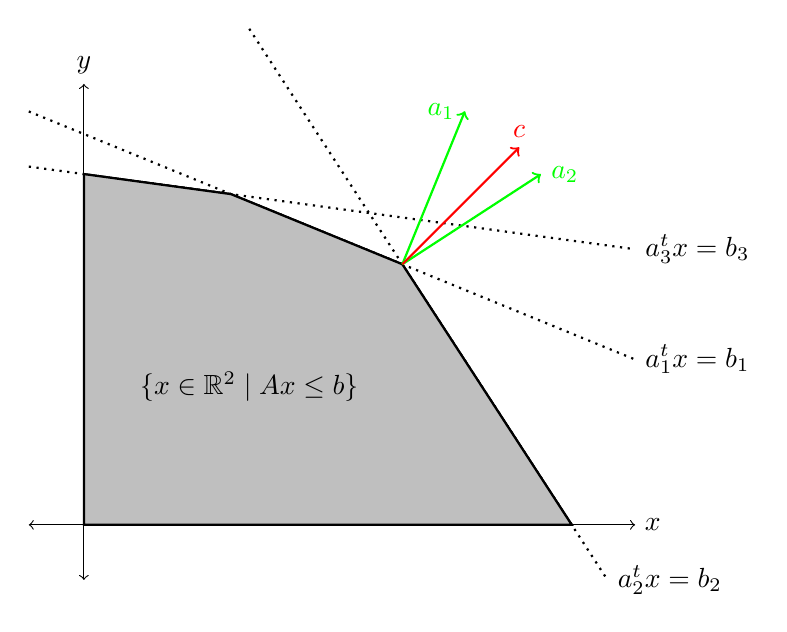
\begin{tikzpicture}[scale=0.7]

  \coordinate (a1) at (-1, 7.5);
  \coordinate (a2) at (10, 3.0);

  \coordinate (b1) at ( 3, 9);
  \coordinate (b2) at (9.5, -1.0);

  \coordinate (c1) at (-1, 6.5);
  \coordinate (c2) at (10, 5.0);

  \coordinate (orig) at (0,0);
  \coordinate (right) at (10,0);
  \coordinate (up) at (0,8);


  \draw[thick, dotted] (a1) -- (a2)node[right]{$a_1^t x = b_1$}; % a
  \draw[thick, dotted] (b1) -- (b2)node[right]{$a_2^t x = b_2$}; % b
  \draw[thick, dotted] (c1) -- (c2)node[right]{$a_3^t x = b_3$}; % c
%  \draw[thick] (d1) -- (d2)node[right]{d};

  \coordinate (ac) at (intersection of a1--a2 and c1--c2);
  \coordinate (ab) at (intersection of a1--a2 and b1--b2);

  \coordinate (cy) at (intersection of c1--c2 and orig--up);
  \coordinate (bx) at (intersection of b1--b2 and orig--right);

  \draw[thick] (cy) -- (ac);
  \draw[thick] (ac) -- (ab);
  \draw[thick] (ab) -- (bx);

  \draw[thick,fill=lightgray] (orig) -- (bx) -- (ab) -- (ac) -- (cy) --cycle;

  \draw[thick,green,->] (ab) -- +(1.136, 2.777) node[left] {$a_1$};  % 0.409,1
  \draw[thick,green,->] (ab) -- +(2.515, 1.635) node[right] {$a_2$}; %1.538,1

  \draw[thick,red,->] (ab) -- +(2.121, 2.121) node[above] {$c$};  % 0.409,1

  \draw[<->] (-1,0) -- (10,0) node[right] {$x$};
  \draw[<->] (0,-1) -- (0,8) node[above] {$y$};

  \draw (3,2.5) node {$\{x \in \R^2 \mid A x \leq b \}$};

%    \foreach \i in {-2,...,7} {
%        \draw (\i,-0.1) -- (\i,0.1); 
%    }
%    \foreach \i in {-2,...,5} {
%        \draw (-0.1, \i) -- (0.1, \i);
%    }

%    \foreach \i in {-0,...,10} {
%       \foreach \j in {-0,...,8} {
%         \fill (\i,\j) circle (1.0pt);
%       }
%    }
  \end{tikzpicture}
\end{center}
\caption{\label{fig::complementary_slackness}
Cost vector $c$ as non-negative combination of rows in $A$.}
\end{figure}

\linebox{\theorem{(Strict Complementary Slackness)}\index{Strict complementary slackness}\label{theorem::strict_complementary}
Let $\max\{c^t x \mid Ax\leq b\}$ and $\min\{b^t y \mid A^t y = c, y\geq 0\}$
be a pair of a primal and a dual linear program that are both feasible and
bounded. Then, for each inequality $a_i^tx \leq b_i$ in $Ax \leq b$ exactly
one of the following two statements holds:
\begin{itemize}
   \item[(a)] The primal LP $\max\{c^t x \mid Ax\leq b\}$ has 
         an optimum solution $x^*$ with $a^t_i x^* < b_i$.
   \item[(b)] The dual LP $\min\{b^t y \mid A^t y = c, y\geq 0\}$
         has an optimum solution $y^*$ with $y^*_i > 0$.
\end{itemize}
}}

\prove 
By complementary slackness, at most one the statements can be true.
Let $\delta = \max\{c^t x \mid Ax\leq b\}$ be the value of an optimum 
solution.
Assume that (a) does not hold. This means that 
\begin{equation*}
   \begin{array}{rcl}
     \max\quad -a^t_i x &&\\
         Ax & \leq & b\\
       -c^t x & \leq & -\delta
   \end{array}
\end{equation*}
has an optimum solution with value $-b_i$.
Hence, also its dual LP
\begin{equation*}
   \begin{array}{rcrcl}
     \min\quad b^ty & - & \delta u &&\\
         A^ty & - & u c & = & -a_i\\
       y & & & \geq & 0\\
     & & u & \geq & 0
   \end{array}
\end{equation*}

must have an optimum
solution of value $-b_i$. Therefore, there are $y \in \R^m$
and $u \in \R$ with $y \geq 0$ and $u \geq 0$ with
$y^t A - u c^t = -a_i^t$ and $y^t b - u \delta = -b_i$.
Let $\tilde y = y + e_i$ (i.e.\ $\tilde y$ arises from $y$ by increasing
the $i$-th entry by one). 
If $u = 0$, then 
$\tilde y^t A = y^t A + a_i^t = 0$ and $\tilde y^t b = y^t b + b_i = 0$,
so if $y^*$ is an optimum solution of $\min\{b^t y \mid A^t y = c, y\geq 0\}$,
then $y^* + \tilde y$ is also an 
optimum solution and has a positive $i$-th entry.
If $u > 0$, then $\frac{1}{u} \tilde y$ is an optimum
solution of $\min\{b^t y \mid A^t y = c, y\geq 0\}$,
(because 
$\frac{1}{u} \tilde y^t A = \frac{1}{u} y^t A + \frac{1}{u} a_i^t = c^t$
and 
$\frac{1}{u} \tilde y^t b = \frac{1}{u}y^t b + \frac{1}{u}b_i = \delta$)
and has a positive $i$-th entry.
\endproof


\linebox{\theorem{
Let $\max\{c^t x \mid Ax\leq b\}$ and $\min\{b^t y \mid A^t y = c, y\geq 0\}$
be a pair of a primal and a dual linear program that are both feasible and
bounded. Then, there are optimum solution $x^*$ and $y^*$  of the LPs such that
for each inequality $a_i^tx \leq b_i$ in $Ax \leq b$ 
either $a^t_i x^* < b_i$ or $y^*_i > 0$ holds.\\
}}

\prove
By Theorem~\ref{theorem::strict_complementary}, for any inequality $a_i^tx \leq b_i$
there is a pair of optimum solutions $x^{(i)} \in \R^n$, $y^{(i)} \in \R^m$ such that
$a^t_i x^{(i)} < b_i$ or $y^{(i)}_i > 0$. Since the convex combination of optimum 
LP solutions is again an optimum solution, we can set
$x^* := \frac{1}{m}\sum_{i=1}^m x^{(i)}$ and $y^* := \frac{1}{m}\sum_{i=1}^m y^{(i)}$ and
get a pair of optimum solutions fulfilling the conditions of the theorem.
\endproof


% See 4.2 of Groetschel




\bigskip

As an application of complementary slackness we consider again the 
{\sc Maximum-Flow Problem}. Let $G$ be a directed graph with $s,t \in V(G)$,
$s \neq t$, and capacities $u: E(G) \to \R_{>0}$.
Here is the LP-formulation of the {\sc Maximum-Flow Problem}:
\begin{equation}\label{eq::maximum_flow_lp2}
\begin{array}{lrcll}
 \max    &       \sum\limits_{e \in \delta^+_G(s)} x_e - \sum\limits_{e \in \delta^-_G(s)} x_e & &\\
\text{s.t.}   & x_e & \geq & 0              & \mbox{for } e \in E(G)\\
              & x_e & \leq & u(e)           &  \mbox{for } e \in E(G)\\
& \sum\limits_{e \in \delta^+_G(v)} x_e - \sum\limits_{e \in \delta^-_G(v)} x_e & = & 0 & 
      \mbox{for } v \in V(G)\setminus\{s,t\}
\end{array}
\end{equation}

By dualizing it, we get
\begin{equation}\label{eq::maximum_flow_dual_lp_complete}
\begin{array}{lrrll}
 \min    &        \sum\limits_{e \in E(G)} u(e)y_e  & &\\
\text{s.t.}   & y_e             & \geq &  0       & \mbox{for } e \in E(G)\\
              & y_e + z_v - z_w & \geq &  0       & \mbox{for } e=(v,w) \in E(G), \{s,t\} \cap \{v,w\} = \emptyset\\
              & y_e + z_v       & \geq &  0       & \mbox{for } e=(v,t) \in E(G), v \neq s\\
              & y_e - z_w       & \geq &  0       & \mbox{for } e=(t,w) \in E(G), w \neq s\\
              & y_e - z_w       & \geq &  1       & \mbox{for } e=(s,w) \in E(G), w \neq t\\
              & y_e + z_v       & \geq & -1       & \mbox{for } e=(v,s) \in E(G), v \neq t\\
              & y_e             & \geq & 1       & \mbox{for } e=(s,t) \in E(G)\\
              & y_e             & \geq & -1      & \mbox{for } e=(t,s) \in E(G)\\
\end{array}
\end{equation}

In a simplified way its dual LP can be written with two dummy variables
$z_s = -1$ and $z_t = 0$:

\begin{equation}\label{eq::maximum_flow_dual_lp}
\begin{array}{lrcll}
 \min    &        \sum\limits_{e \in E(G)} u(e)y_e  & &\\
\text{s.t.}   & y_e             & \geq &  0       & \mbox{for } e \in E(G)\\
              & y_e + z_v - z_w & \geq &  0       & \mbox{for } e=(v,w) \in E(G)\\
              & z_s             &  =  &  -1      &\\
              & z_t             &  =  &   0      &\\
\end{array}
\end{equation}






We will use the dual LP to show the Max-Flow-Min-Cut-Theorem.
%Let $G$ be a directed graph with edge capacities 
%$u:E(G) \to \R_{> 0}$.
We call a set $\delta^+(R)$ with $R \subset V(G)$, 
$s \in R$ and $t \not \in R$ 
an $s$-$t$-cut.{\index{s-t-cut@$s$-$t$-cut}}


\linebox{
\begin{theorem}(Max-Flow-Min-Cut-Theorem){\index{Max-Flow-Min-Cut-Theorem}} 
Let $G$ be a directed graph with edge capacities 
$u:E(G) \to \R_{> 0}$. Let $s,t \in V(G)$ be two different vertices.
Then, the minimum of all capacities of $s$-$t$-cuts equals the maximum
value of an $s$-$t$-flow.
\end{theorem}
}

\prove
If $x$ is a feasible solution of the primal problem (\ref{eq::maximum_flow_lp2})
(i.e.\ $x$ encodes an $s$-$t$-flow) and 
$\delta^+(R)$ is an $s$-$t$-cut, then
\[
   \sum\limits_{e \in \delta^+_G(s)}  x_e - \sum\limits_{e \in \delta^-_G(s)}  x_e
      =  \sum_{v \in R } \left( \sum\limits_{e \in \delta^+_G(v)}  x_e - 
                              \sum\limits_{e \in \delta^-_G(v)}  x_e \right)
      = \sum\limits_{e \in \delta^+_G(R)} x_e -  \sum\limits_{e \in \delta^-_G(R)} x_e
      \leq  \sum\limits_{e \in \delta^+_G(R)} u(e).
\]
The first equation follows from the flow conservation rule
(i.e.\ $\sum\limits_{e \in \delta^+_G(v)} x_e - \sum\limits_{e \in \delta^-_G(v)} x_e = 0$)
applied to all vertices in $R \setminus \{s\}$ and the second one
from the fact that flow values on edges inside $R$ cancel out in the sum.
The last inequality follows from the fact that flow values are between
$0$ and $u$.

Thus, the capacity of any $s$-$t$-cut is an 
upper bound for the value of an $s$-$t$-flow. We will show that
for any maximum $s$-$t$-flow there is an $s$-$t$-cut whose capacity
equals the value of the flow.

Let $\tilde x$ be an optimum solution of the primal problem (\ref{eq::maximum_flow_lp2})
and $\tilde y$, $\tilde z$ be an optimum solution of the dual problem
(\ref{eq::maximum_flow_dual_lp}). In particular $\tilde x$ defines a maximum
$s$-$t$-flow. 
Consider the set
$R := \{v \in V(G) \mid \tilde z_v \leq -1\}$. Then $s \in R$ and $t \not \in R$.

If $e = (v,w) \in \delta_G^+(R)$, then $\tilde z_v < \tilde z_w$, so 
$\tilde y_e \geq \tilde z_w - \tilde z_v > 0$. By complementary slackness
this implies $\tilde x_e = u(e)$. On the other hand, if $e = (v,w) \in \delta_G^-(R)$,
then $\tilde z_v > \tilde z_w$ and hence 
$\tilde y_e + \tilde z_v - \tilde z_w  \geq \tilde z_v - \tilde z_w > 0$, so again
by complementary slackness $\tilde x_e = 0$. This leads to:
\[
   \sum\limits_{e \in \delta^+_G(s)} \tilde x_e - \sum\limits_{e \in \delta^-_G(s)} \tilde x_e
      =  \sum_{v \in R } \left( \sum\limits_{e \in \delta^+_G(v)} \tilde x_e - 
                              \sum\limits_{e \in \delta^-_G(v)} \tilde x_e \right)
      = \sum\limits_{e \in \delta^+_G(R)} \tilde x_e -  \sum\limits_{e \in \delta^-_G(R)} \tilde x_e
      = \sum\limits_{e \in \delta^+_G(R)} u(e).
\]
\endproof

\paragraph{Remark.} In the proof above, we defined $R := \{v \in V(G) \mid \tilde z_v \leq -1\}$. Instead, we could have used $R := \{v \in V(G) \mid \tilde z_v \leq \alpha\}$ for any $-1\le \alpha <0$. The same arguments show that $s\in R$, $t\notin R$, $x_e=u_e$ for $e\in \delta_G^+(R)$, and $x_e=0$ for $e\in \delta_G^-(R)$. Moreover, observe that for any minimum cut $R\subseteq V\setminus\{t\}$, $s\in R$, setting $z_v=-1$ for $v\in S$, $z_v=0$ for $v\notin S$, and $y_e=1$ for $e\in \delta_G^+(R)$ and $w_e=0$ otherwise gives a dual optimal solution. This can be verified by checking feasibility and complementarity with the optimal flow $x$.

 %Let $A=\{z_v\mid v\in V, z_v<0\}\subseteq [-1,0)$ be the set of different values 

%TODO: Goldberg-Tarjan as a dual algorithm

%%%%%%%%%%%%%%%%%%%%%%%%%%
\section{The Structure of Polyhedra}
%%%%%%%%%%%%%%%%%%%%%%%%%%

\subsection{Mappings of Polyhedra}

\linebox{
\proposition{
Let $A \in \R^{m \times (n+k)}$ and $b \in \R^m$. Then the set 
\[
   P = \{x \in \R^n \mid \exists y \in \R^k: A {x \choose y} \leq b\}
\]
is a polyhedron.\\
}
}

\prove
Exercise.
\endproof

{\bf Remark:} The set $P = \{x \in \R^n \mid \exists y \in \R^k: A {x \choose y} \leq b\}$
is called a {\hi projection} of{\index{Projection of a polyhedron}}
$\{z \in \R^{n+k} \mid A z \leq b\}$ to $\R^n$.


More generally, the image of a polyhedron $\{x \in \R^n \mid Ax \leq b\}$ 
under an {\hi affine linear mapping}{\index{Affine linear mapping}}
 $f: \R^n \to \R^k$, which is given by 
$D \in \R^{k \times n}$, $d \in \R^k$ and $x \mapsto Dx + d$  is also a polyhedron:

\linebox{
\corollary{
Let $A \in \R^{m \times n}$, $b \in \R^m$, $D \in \R^{k \times n}$ and 
$d \in \R^k$.
Then 
\[
   \{y \in \R^k \mid \exists x \in \R^n: Ax \leq b \text{ and } y = Dx + d\}
\]
is a polyhedron.\\
}
}

\prove
Note that
\small
\begin{eqnarray*}
  && \Bigg\{y \in \R^k     \mid \exists x \in \R^n: Ax \leq b \text{ and } y = Dx + d\bigg\}\\
 & = & \left\{y \in \R^k  \mid \exists x \in \R^n: \left( \begin{array}{cc} A & 0 \\ D & -I_k \\ -D & I_k \end{array}\right)
  {x \choose y}
   \leq \left( \begin{array}{c} b \\ -d \\ d \end{array}\right)  \right\} 
\end{eqnarray*}
\normalsize
and apply the previous proposition.
\endproof

\subsection{Faces}

\linebox{
\definition{
Let $P=\{x \in \R^n \mid Ax \leq b\}$ be a 
non-empty polyhedron and $c \in \R^n\setminus\{0\}$.
\begin{itemize}
\item[(a)] For $\delta := \max\{c^t x \mid x \in P\} < \infty$, the set
  $\{x \in \R^n \mid c^tx=\delta\}$ is called 
  {\hi supporting hyperplane}{\index{Supporting hyperplane}}
of $P$.
\item[(b)] A set $X\subseteq \R^n$ is called {\hi face}{\index{Face}} of 
  $P$ if $X=P$ or if there is a supporting hyperplane $H$ of $P$
  such that $X = P \cap H$.
\item[(c)] If $\{x'\}$ is a face of $P$, we call $x'$ 
  {\hi vertex of $P$}{\index{Vertex}}
  or {\hi basic solution}{\index{Basic solution}}
  of the system $Ax\leq b$.
\end{itemize}
}
}

% {\bf Remark:} For example, a non-empty polyhedron of the form
% $P = \{x \in \R^n \mid A x = b\}$, which is in fact a linear subspace,
% has only one face, namely $P$ itself. 
% To see this, assume that there is a set 
% $F = \{x \in P \mid c^tx = \delta\} \subsetneq P$ for
% $c\in \R^n$ and $\delta \in \R$ such that $c^t x \leq \delta$
% for all $x \in P$. Then, for $x \in F$ and $y \in P \setminus F$,
% we have $c^t(2x -y) = 2 \delta - c^t y > \delta$, so 
% $2x - y \not\in P$. On the other hand, $A(2x - y) = 2b - b = b$,
% which would imply $2x - y \in P$. Hence, we have a contradiction, so,
% in this case, $P$ does not contain a proper subset as a face.


\linebox{
\proposition{\label{proposition::faces}
Let $P = \{x \in \R^n \mid Ax \leq b\}$ be a non-empty
polyhedron and $F \subseteq P$.
Then, the following statements are equivalent:
\begin{itemize}
\item[(a)] $F$ is a face of $P$.
\item[(b)] There is a vector $c \in \R^n$ such that
    $\delta := \max\{c^t x \mid x \in P\} < \infty$ and 
    $F=\{x \in P \mid c^t x= \delta\}$.
\item[(c)] There is a subsystem $A' x \leq b'$ of $Ax \leq b$ such that
    $F = \{x \in P \mid A'x = b'\} \neq \emptyset$.
\end{itemize}
}}

\prove % Proposition 2.7 von Stephan
\begin{description}
   \item[``(a) $\Rightarrow$ (b)'':] 
       Let $F$ be a face of $P$.
       If $F=P$, then $c=0$ yields $F=\{x \in P \mid c^t x= 0\}$.
       If $F \neq P$, then there must be a $c \in \R^n$ such that for
       $\delta := \max\{c^t x \mid x \in P\} (< \infty)$ we have 
       $F = \{x \in \R^n \mid c^tx=\delta\} \cap P 
          = \{x \in P \mid c^t x= \delta\}$.
   \item[``(b) $\Rightarrow$ (c)'':] Let $c$, $\delta$ and $F$ be as 
        described in (b). Consider the LP $\max c^t x$ s.t. $Ax\le b$. Thus, $F$ is exactly the set of optimal solutions to this LP. 

        Since the LP is feasible and bounded, there exists a dual optimal solution $y\in\R^m$ such that $b^t y=c^t x$, $A^t y=c$, $y\ge 0$. Let $I=\{j\mid y_i>0\}$ denote the support of $y$, and let $A'x=b'$ be the subsystem formed by the equalities $A_I x=b_I$. By complementary slackness (Theorem~\ref{theorem::ComplementaySlackness}), $x$ is an optimal solution to the LP if and only if $a_i x=b_i$ for $i\in I$. Thus, we obtain $F= \{x \in P \mid A'x = b'\}$. 
        \iffalse 



        Let $A'x\leq b'$ be a maximal subsystem 
        of $Ax\leq b$ such that $A'x = b'$ for all
        $x \in F$. Hence $F \subseteq \{x \in P \mid A'x = b'\}$
        and it remains to show that 
        $F \supseteq \{x \in P \mid A'x = b'\}$.
        Let $\tilde A x \leq \tilde b$ be the inequalities in
        $Ax\leq b$ that are not contained in $A'x\leq b'$. 
        Denote the inequalities of $\tilde A x \leq \tilde b$ by
        $\tilde a_j^t x \leq \tilde b_j$ ($j=1,\dots,k$).
        Hence, for each $j=1,\dots,k$ 
        we have an $x_j \in F$ with 
        $\tilde a_j x_j < \tilde b_j$.
        
        If $k > 0$, we set $x^* := \frac{1}{k}\sum_{j=1}^k x_j$.
        Otherwise let $x^*$ be an arbitrary element of $F$.
        In any case, we have $\tilde a_j^t x^* < \tilde b_j$ for all 
        $j \in \{1,\dots,k\}$.

        Consider an arbitrary $y \in P \setminus F$. We have to show
        that $A'y \neq b'$. 

        Because of $y \in P \setminus F$ we know that $c^t y < \delta$.

        Choose $\epsilon > 0$ with 
        $\epsilon < \frac{\tilde b_j - \tilde a_j^t x^*}{\tilde a_j^t (x^* - y)}$
        for all $j \in \{1,\dots,k\}$ with $\tilde a_j^t x^* > \tilde a_j^t y$
        (note that all these upper bounds on $\epsilon$ are positive).

         Set $z := x^* + \epsilon(x^* - y)$ (see Figure~\ref{fig::proposition_proof_face}).
         Then $c^t z > \delta$, so
         $z \not\in P$. Therefore, there must be an inequality $a^t x \leq \beta$
         of the system $A x \leq b$ such that $a^t z > \beta$. We claim that
         this inequality cannot belong to $\tilde A x \leq \tilde b$.
         To see this assume that $a^t x \leq \beta$ belongs to $\tilde A x \leq \tilde b$.
         If $a^t x^* \leq a^t y$ then
         \[
            a^t z = a^tx^* + \epsilon a^t(x^* - y) \leq a^tx^* < \beta.
         \]
         But if $a^t x^* > a^t y$ then
         \[
            a^t z = a^tx^* + \epsilon a^t(x^* - y) 
                  < a^tx^* + \frac{\beta - a^t x^*}{a^t (x^* - y)} 
                             a^t(x^* - y) = \beta.
         \]
         In both cases, we get a contradiction, so 
         the inequality $a^t x \leq \beta$ belongs to $A' x \leq b'$. 
         Therefore,
         $a^t y = a^t(x^* + \frac{1}{\epsilon}(x^* - z)) 
           = (1+\frac{1}{\epsilon})\beta - \frac{1}{\epsilon} a^t z
         < \beta$,
         which means that $A'y \neq b'$.
         \fi
   \item[``(c) $\Rightarrow$ (a)'':] 
        Let $A' x \leq b'$ be a subsystem of $Ax \leq b$ such that
        $F = \{x \in P \mid A'x = b'\}$.
        Let $c^t$ be the sum of all row vectors of
        $A'$, and let $\delta$ be the sum of the
        entries of $b'$. Then, $c^t x \leq \delta$ for all $x \in P$
        and $F = P \cap H$ with
        $H = \{x \in \R^n \mid c^t x=\delta\}$. \endproof
%\fi
\end{description}


%\ifdefined\InitialVersion{}\else



\iffalse

\begin{figure}[htb]
\begin{center}
  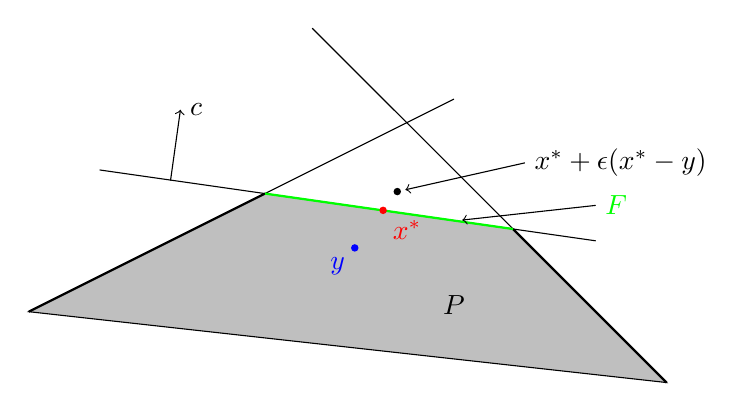
\begin{tikzpicture}[scale=0.9]
    \coordinate (a1) at (1,1);
    \coordinate (a2) at (7,4);

    \coordinate (b1) at (2,3);
    \coordinate (b2) at (9,2);

    \coordinate (c1) at (5,5);
    \coordinate (c2) at (10,0);

    \coordinate (ab) at (intersection of a1--a2 and b1--b2);
    \coordinate (bc) at (intersection of b1--b2 and c1--c2);




   \draw[fill=lightgray] (a1) -- (ab) -- (bc) -- (c2) --cycle;

   \draw (7,  1.1) node{$P$};


    \draw[thick] (a1) -- (ab);
    \draw (ab) -- (a2);

    \draw (b1) -- (ab);
    \draw (bc) -- (b2);

    \draw (c1) -- (bc);
    \draw[thick] (bc) -- (c2);

    \draw[thick, green] (ab) -- (bc);



    \fill[red]   (6,   2.43) circle (1.5pt) node[below right, red]{$x^*$};
    \fill[blue]  (5.6, 1.9 ) circle (1.5pt) node[below left, blue]{$y$};

    \fill[black] (6.2, 2.695) circle (1.5pt);

    \draw[<-, shorten <=3pt] (6.2, 2.695) -- (8, 3.1) node[right, black]{$ x^* + \epsilon(x^* - y)$};


    \draw[<-, shorten <=3pt] (7,2.28) -- (9, 2.5) node[right, green] {$F$};

    \draw[->] (3, 2.85) -- (3.14, 3.85) node[right] {$c$};

%    \coordinate (c) at (intersection of c1x--c1y and c3x--c3y);

  \end{tikzpicture}
\end{center}
\caption{\label{fig::proposition_proof_face}
Illustration of part ``(b) $\Rightarrow$ (c)'' of the proof of 
Proposition~\ref{proposition::faces}}
\end{figure}


\fi













The following corollary summarizes direct consequences of the 
previous proposition:

\linebox{
\corollary{\label{Corollary::faces}
Let $P\neq \emptyset$ be a polyhedron and $F$ a face of $P$.
\begin{itemize}
\item[(a)] Let $c \in \R^n$ be a vector such that
  $\max\{c^t x \mid x \in P\} < \infty$. Then the set of all vectors 
  $x$ where the maximum of $c^t x$ over $P$ is attained is a face of $P$.
\item[(b)] $F$ is a polyhedron.
\item[(c)] A subset $F' \subseteq F$ is a face of $F$ 
  if and only if $F'$ is a face of $P$.
\item[(d)] If $P$ is of the form $P = \{x \in \R^n \mid A x = b\}$, 
  so it is in fact a linear subspace, then $P$ has only one face, 
  namely $P$ itself. 
   \endproof
\end{itemize}
}
}



We are in particular interested in the largest and the
smallest faces of a polyhedron.

%\prove
%\begin{itemize}
%\item[(a)] Follows from the implication ``(b) $\Rightarrow$ (a)'' of 
%     Proposition~\ref{proposition::faces}.
%\item[(b)]
%\item[(c)]
%\end{itemize}
%\endproof

\subsection{Facets}


\linebox{\definition{
Let $P$ be a polyhedron. A {\hi facet}{\index{Facet}} of $P$ is an (inclusion-wise) maximal
face $F$ of $P$ with $F\neq P$. An inequality $c^t x \leq \delta$ is 
{\hi facet-defining}{\index{Facet-defining}}
for $P$ if $c^t x \leq \delta$ for all $x \in P$
and $\{x \in P \mid c^t x = \delta\}$ is a facet.\\
}}

%Description of polyhedra by facet-defining inequalities.

\linebox{
\theorem{\label{theorem::facetdefining}
Let $P \subseteq \{x \in \R^n \mid Ax=b\}$ be a non-empty polyhedron
of dimension $n - \mbox{rank}(A)$. Let $A' x \leq b'$ be a minimal
system of inequalities such that $P = \{x \in \R^n \mid Ax=b, A' x \leq b'\}$.
Then, every inequality in $A'x \leq b'$ is facet-defining for $P$ and
every facet of $P$ is given by an inequality of $A' x \leq b'$.\\
}
}





\prove %Prop 2.11 from Stephan
If $P = \{x \in \R^n \mid Ax=b\}$, then $P$ does not have a facet
(the only face of $P$ is $P$ itself, see Corollary~\ref{Corollary::faces}~(d)),
so both statements are trivial.

Hence assume that $P \neq \{x \in \R^n \mid Ax=b\}$.

Let $A' x \leq b'$ be a minimal system of inequalities such that
$P=\{x \in \R^n \mid Ax=b, A'x \leq b' \}$. Let $a^t x \leq \beta$
be an inequality in $A' x \leq b'$, and let $A'' x \leq b''$ be the
rest of the system $A' x \leq b'$ without $a^t x \leq \beta$.

We will show that $a^t x \leq \beta$ is facet-defining.

Let $y \in \R^n$ be a vector with $Ay = b$, $A'' y \leq b''$ and
 $a^t y > \beta$. Such a vector exists because otherwise 
$A'' y \leq b''$ would be a smaller system of inequalities than
$A' \leq b'$ with
$P=\{x \in \R^n \mid Ax=b, A'' x\leq b'' \}$, which is a contradiction
to the definition of $A' x \leq b'$.

Moreover, let $\tilde y \in P$ be a vector with $A' \tilde y < b'$
(such a vector $\tilde y$ exists because $P$ is full-dimensional in the 
linear subspace $\{x \in \R^n \mid Ax = b\}$ and because of the
minimality of the system $A' x \leq b'$).
Consider the vector
\[
   z = \tilde y + \frac{\beta - a^t \tilde y}{a^ty - a^t \tilde y}(y - \tilde y).
\]
Then, $a^t z = a^t  \tilde y + \frac{\beta - a^t \tilde y}{a^ty - a^t \tilde y}
          (a^t y - a^t \tilde y) = \beta$. 
Furthermore, $0 < \frac{\beta - a^t \tilde y}{a^ty - a^t \tilde y} < 1$. Thus,
$z$ is the convex combination of $\tilde y$ and $y$, so $Az = b$ and $A'' z \leq b''$.
Therefore, we have $z \in P$.

Set $F := \{x \in P \mid a^t x = \beta\}$. Then, $F \neq \emptyset$
(because $z \in F$), and $F \neq P$ because $\tilde y \in P \setminus F$.
Hence, $F$ is a face of $P$. It is also a facet because 
$a^t x \leq \beta$ is the only inequality of $A' x \leq b'$ that is
met by all elements of $F$ with equality (e.g.\ the vector $z \in F$
fulfills all inequalities in $A''x \leq b''$ with strict inequality).

On the other hand, by Proposition~\ref{proposition::faces}
any facet is defined by an inequality of $A' x \leq b'$.
\endproof

\linebox{
\corollary{
Let $P\subseteq \R^n$ be a polyhedron.
\begin{itemize}
   \item[(a)] Every face $F$ of $P$ with $F \neq P$ is the intersection
              of facets of $P$.
   \item[(b)] The dimension of every facet of $P$ is $\text{dim}(P) - 1$. \endproof
\end{itemize}
}
}


In particular, this means that the smallest possible representation
of a full-dimensional polyhedron $P = \{x \in \R^n \mid Ax \leq b\}$
is unique (up to swapping inequalities and multiplying inequalities
with positive constants). 
If possible, we want to describe any polyhedron by facet-defining inequalities
because according to the Theorem~\ref{theorem::facetdefining},
this gives such a smallest possible
description of the polyhedron (with respect to the number of inequalities).

\subsection{Minimal Faces}

\linebox{
\definition
A face $F$ of a polyhedron $P$ is called a {\hi minimal face} if there
is no face $F'$ of $P$ with
$F' \subsetneq F$.{\index{Minimal face}}\\
}

\linebox{
\proposition{\label{proposition::minimal_faces}
%Minimal faces are of the form $\{x \in \R^n \mid A'x = b'\}$.
Let $P=\{x \in \R^n \mid Ax\leq b\}$ be a polyhedron. A non-empty
set $F\subseteq P$ is a minimal face of $P$ if and only if there is
a subsystem $A'x \leq b'$ of $Ax\leq b$ with 
$F=\{x \in \R^n \mid A'x=b'\}$.\\
}
}

\prove
``$\Rightarrow$:''
Let $F$ be a minimal face of $P$. 
By Proposition~\ref{proposition::faces}, we know that there is
a subsystem $A'x \leq b'$ of $Ax\leq b$ with 
$F=\{x \in P \mid A'x=b'\}$. Choose $A'x \leq b'$ maximal with this
property. Let $\tilde A x\leq \tilde b$ be a minimal subsystem of
$Ax\leq b$ such that $F=\{x \in \R^n \mid A'x=b', \tilde A x\leq \tilde b\}$.

We have to show the following claim:

{\bf Claim:} $\tilde A x\leq \tilde b$ is an empty system of inequalities.


{\bf Proof of the Claim:} Assume that $a^t x \leq \beta$ is an
inequality in $\tilde A x\leq \tilde b$.
The inequality $a^t x \leq \beta$ is not redundant, so 
by Theorem~\ref{theorem::facetdefining}, 
$F'=\{x \in \R^n \mid A' x = b', \tilde A x\leq \tilde b, a^t x = \beta\}$ is a facet of
$F$, and hence, by Corollary~\ref{Corollary::faces}, $F'$ is s face of $P$.
On the other hand, we have $F'\neq F$, because $a^t x = \beta$ is not valid for
all elements of $F$ (otherwise we could have added $a^tx \leq \beta$ to the set of
inequalities $A'x \leq b'$). This is a contradiction to the minimality of $F$.
This proves the claim.


``$\Leftarrow$:'' Assume that $F = \{x \in \R^n \mid A' x = b'\} \subseteq P$
(for a subsystem $A'x \leq b'$ of $Ax\leq b$) is non-empty.

Then, $F$ cannot contain a proper subset as a face
(see Corollary~\ref{Corollary::faces}~(d)).

Moreover, $F = \{x \in \R^n \mid A' x = b'\} = \{x \in P \mid A' x = b'\}$,
so by Proposition~\ref{proposition::faces} the set $F$ is a face of $P$.
Since any proper subset of $F$ that is a face of $P$ would also be 
a face of $F$ and we know that $F$ does not contain proper subsets as
faces, $F$ is a minimal face of $P$.
\endproof

\linebox{
\corollary{
Let $P = \{x \in \R^n \mid Ax \leq b\}$ be a polyhedron.
Then the minimal faces of $P$ have dimension $n - \mbox{rank}(A)$.\\
%All minimal faces are of the same dimension.
}}


\prove
Let $F$ be a minimal face of $P = \{x \in \R^n \mid Ax \leq b\}$.
By Proposition~\ref{proposition::minimal_faces}, it can be written as
$F = \{x \in \R^n \mid A' x = b'\}$ for a subsystem 
$A'x \leq b'$ of $Ax \leq b$. If $A'$ had smaller rank than $A$, we could
add a new constraint $a^t x \leq \beta$ of $Ax \leq b$ 
to $A'x \leq b'$ such that $a^t$
is linearly independent to all rows of $A'$. Then,
$\{x \in \R^n \mid A' x = b', a^t x = \beta\} \subsetneq F$ would be a
face of $F$ and thus a face of $P$.
This is a contradiction to the minimality of $F$.
Hence, we can assume that $\mbox{rank}(A') = \mbox{rank}(A)$.

Therefore, $\mbox{dim}(F) = n - \mbox{rank}(A') = n - \mbox{rank}(A)$.
\endproof


\linebox{
\proposition{\label{theorem::vertex}
Let $P = \{x \in \R^n \mid Ax \leq b\}$ be a polyhedron and $x' \in P$.
Then, the following statements are equivalent:
\begin{itemize}
\item[(a)] $x'$ is a vertex of $P$.
\item[(b)] There is a subsystem $A' x \leq b'$ of $Ax \leq b$ of $n$
inequalities such that the rows of $A'$ are linearly independent and
  $\{x'\} = \{x \in P \mid A'x = b'\}$.
\item[(c)] $x'$ cannot be written as a convex combination of vectors in 
  $P \setminus\{x'\}$.
\item[(d)] There is no non-zero vector $d \in \R^n$ such that
  $\{x' + d, x' - d\} \subseteq P$.
\end{itemize}
}}


\prove
\begin{description}
   \item[``(a) $\Leftrightarrow$ (b)'':] 
          By Proposition~\ref{proposition::minimal_faces}, $x'$ is a vertex if and only if
          there is a subsystem $A'x \leq b'$ of $Ax\leq b$ with 
          $\{x'\} = \{x \in \R^n \mid A'x=b'\}$. Since $\{x'\}$ is of dimension $0$, this is
          the case if and only if the statement in (b) holds.
   \item[``(b) $\Rightarrow$ (c)'':] Let $A' x \leq b'$ be a subsystem of
          $n$ inequalities of $Ax \leq b$ 
          such that the rows of $A'$ are linearly independent and
          $\{x'\} = \{x \in P \mid A'x = b'\}$. Assume that $x'$ can be 
          written as a convex combination $\sum_{i=1}^{k}\lambda_i x^{(i)}$ of vectors
          $x^{(i)} \in P \setminus\{x'\}$ (so $\lambda_i \geq 0$ for $i \in \{1,\dots,k\}$
          and $\sum_{i=1}^{k}\lambda_i = 1$). If we had $a^t x^{(i)} < \beta$ for any
          inequality $a^t x \leq \beta$ in $A' x \leq b'$ and 
          $i \in \{1,\dots,k\}$, then $a^t x' = \sum_{i=1}^{k}\lambda_i a^t x^{(i)} < \beta$,
          which is a contradiction. But then, we have 
          $x^{(i)} \in \{x \in P \mid A'x = b'\} = \{x'\}$ for all $i \in \{1,\dots,k\}$, which
          is a contradiction, too.
   \item[``(c) $\Rightarrow$ (d)'':] If $\{x' + d, x' - d\} \subseteq P$, then 
          $x' = \frac{1}{2}((x' + d) + (x' - d))$, so $x'$ can be written as a convex
          combination of vectors in $P \setminus\{x'\}$.
   \item[``(d) $\Rightarrow$ (b)'':] Let $A' x \leq b'$ be a maximal subsystem of $Ax \leq b$ 
          such that $A'x' = b'$. Assume that $A'$ does not contain $n$ linearly independent 
          rows. Then, there is a vector $d$ that is orthogonal to all rows in $A'$. 
          Hence, for any $\epsilon > 0$, we have $A'(x' + \epsilon d) = A'(x' - \epsilon d) = b'$.
          For any inequality $a^tx \leq \beta$ that is in $Ax\leq b$ but not in $A'x\leq b'$, 
          we have $a^t x' < \beta$.
          Therefore, if $\epsilon > 0$ is sufficiently small, $a^t (x' + \epsilon d) \leq \beta$
          and $a^t (x' - \epsilon d) \leq \beta$ are valid for inequalities $a^tx \leq \beta$
          in $Ax\leq b$ but not in $A'x\leq b'$.
          In other words, we have $(x' + \epsilon d) \in P$ and $(x' - \epsilon d) \in P$.
\endproof
\end{description}



\linebox{
\definition{
A polyhedron is called {\hi pointed}{\index{Pointed polyhedron}} if
it is empty or 
all minimal faces of it are of dimension $0$.\\
}}





{\bf Examples:}\vspace*{-4mm}
\begin{itemize}
\item Polytopes are pointed.\\
To see this, consider a non-empty polytope $P=\{x \in \R^n \mid Ax \leq b\}$.
If $\mbox{rank}(A) < n$, then there is a vector $\tilde x \in \R^n$ such that
$A \tilde x = 0$. But then for any $x \in P$ and $K \in \R$, we have
$x + K\tilde x \in P$, which is a contradiction to the assumption that $P$
fits into a ball of finite radius. Hence we have $\mbox{rank}(A)=n$, so $P$ is 
pointed.
\item Polyhedra $P$ that can be written as 
  $P = \{x \in \R^n \mid Ax=b, x\geq 0\}$ are pointed.\\
This can be seen by writing $P$ as 
$P=\{x \in \R^n \mid \left( \begin{array}{c} A \\ -A\\ -I_n \end{array}\right) x \leq
\left( \begin{array}{c} b \\ -b\\ 0 \end{array}\right)
 \}$.
% (where $I$ is the $n\times n$ identity matrix). 
Obviously, the
matrix $\left( \begin{array}{c} A \\ -A\\ -I_n \end{array}\right)$ has rank $n$,
hence $P$ is pointed.
\end{itemize}

\linebox{
\corollary{\label{corollary::VertexOptimal}
If the linear program $\max\{c^t x \mid Ax\leq b\}$ is feasible and bounded and
the polyhedron $P = \{x \in \R^n \mid Ax\leq b\}$ is pointed, then there is
a vertex $x'$ of $P$ such that $c^t x' = \max\{c^t x \mid Ax\leq b\}$. \endproof\\
}
}

\subsection{Cones}\label{sec::cones}

\linebox{
\theorem{(Carath\'{e}odory's Theorem)}\label{thm:caratheodory}
{\index{Caratheodory's Theoremm@{Carath\'{e}odory's Theorem}}}
If $X \subseteq \R^n$ is a finite set of vectors
and $c \in \text{cone}(X)$ then
there are linearly independent vectors 
$a_1,\dots,a_k \in X$
such that $c \in \text{cone}(\{a_{1},\dots,a_{k}\})$.\\
}

\prove
Let $\{a_{1},\dots,a_{k}\}$ be an inclusion-wise minimal set
of vectors in $X$ such that $c \in \text{cone}(\{a_{1},\dots,a_{k}\})$.
This means that there are positive numbers $\lambda_1,\dots,\lambda_k$
such that $c = \sum_{i=1}^k \lambda_i a_i$.

We show that the vectors $a_1,\dots,a_k$ are linearly independent.
If this is not the case, there are numbers $\gamma_1,\dots,\gamma_k$
such that $ \sum_{i=1}^k \gamma_i a_i = 0$. We can assume that at least
one $\gamma_i$ is positive. Choose $\sigma$ maximal such that  
$\lambda_i - \sigma \gamma_i \geq 0$ for all $i \in \{1,\dots, k\}$.
%$\sigma = \max\{ \frac{\lambda_i}{\gamma_i} \mid i \in \{1,\dots, k\}\}$.
Then, in particular, for at least on on $i \in \{1,\dots, k\}$, we have
$\lambda_i - \sigma \gamma_i = 0$.
Therefore, $\sum_{i=1}^k (\lambda_i - \sigma \gamma_i) a_i$ is a representation
of $c$ with less vectors, which is a contradiction to the minimality
of the set $\{a_{1},\dots,a_{k}\}$.
\endproof


\linebox{
\theorem{(Fundamental Theorem of Linear Inequalities)
{\index{Fundamental Theorem of Linear Inequalities}}\label{theorem::fundemental}
Let $a_1,\dots,a_m,c \in \R^n$ be vectors and 
let $t$ be the dimension of the subspace of $\R^n$ spanned by
$a_1,\dots,a_m,c$ 
(so $t$ is the rank of the matrix whose rows are
 $a_1^t,\dots,a_m^t,c^t$).
Then, exactly one of the following statements is true:
\begin{itemize}
\item[(a)] %$c \in \mbox{cone}(\{a_1,\dots,a_m\})$
     $c$ can be written as a non-negative combination of
     linearly independent vectors from $a_1^t,\dots,a_m^t$.
\item[(b)] There is a hyperplane $\{x \in \R^n \mid u^t x = 0\}$
     (for a non-zero vector $u \in \R^n$) containing $t-1$ linearly
     independent vectors from $a_1,\dots,a_m$ such that $a_i^t u \geq 0$
     for $i \in \{1,\dots,m\}$ and $c^t u < 0$.
\end{itemize}
}
}

\prove
Obviously, at most one of the statements can be valid. 
Let $A$ be the matrix with rows $a_1^t,\dots,a_m^t$.

If $c \in \mbox{cone}(\{a_1,\dots,a_m\})$ then by the previous
theorem, $c$ can be written as a non-negative combination of
linearly independent vectors from $a_1^t,\dots,a_m^t$.

Hence, assume that
$c \not\in \mbox{cone}(\{a_1,\dots,a_m\})$, so there is no vector $v \in \R^m$,
$v \geq 0$ such that $c^t = v^t A$. By Farkas' Lemma (Theorem~\ref{theorem::farkas2}),
this implies that there is a vector $\tilde u \in \R^n$ such that 
$A \tilde u \geq 0$ and $c^t \tilde u < 0$.
This implies that the following LP (with $u \in \R^n$
as variable vector) has a feasible solution:
\[
\begin{array}{rrcl}
\max        &  c^t u &       &    \\
\mbox{s.t.} &  c^t u & \leq  & -1 \\
            & -c^t u & \leq  & 1 \\
            & -Au    & \leq  & 0  \\
\end{array}
\]
Moreover, the LP is bounded 
(-1 is the value of an optimum solution).
Hence, the optimum is attained on a face of the 
solution polyhedron. 
By Theorem~\ref{proposition::minimal_faces}, we can write a
minimal face where the optimum solution value is attained
as a set
$F = \{ u \in \R^n \mid A' u = b' \}$ where $A' u \leq b'$ is a 
subsystem of $c^t u \leq  -1$, $-c^t u  \leq 1$, $-Au \leq 0$
consisting of $t$ linearly independent vectors. Hence, any vector
$u \in F$ fulfills the condition of (b).
\endproof


\linebox{
\theorem{(Farkas-Minkowski-Weyl Theorem)\label{theorem::FarkasMinkoswkiWeyl}{\index{Farkas-Minkowski-Weyl Theorem}}
A convex cone is polyhedral if and only if it is finitely generated.\\
}
}

\prove
``$\Leftarrow$:'' % As in \cite{Sch86}.
Let $a_1,\dots,a_m \in \R^n$ be vectors. We have to show that
$\mbox{cone}(\{a_1,\dots,a_m\})$ is polyhedral. W.l.o.g.\ we can assume
that the vectors $a_1,\dots,a_m$ span the vector space $\R^n$. Consider
the set $\mathcal{H}$ 
of half-spaces $H_u = \{x \in \R^n \mid u^t x \leq 0\}$ such that 
for each $H_u \in \mathcal{H}$ the following conditions hold:
\begin{itemize}
   \item $\{a_1,\dots,a_m\} \subseteq H_u$, and
   \item There are $n-1$ linearly independent vectors
         $a_{i_1},\dots,a_{i_{n-1}}$ in $\{a_1,\dots,a_m\}$
         such that $u^t a_{i_j} = 0$ for $j \in \{1,\dots,n-1\}$
\end{itemize}
The set $\mathcal{H}$ is finite because there are at most
$m \choose n-1$ such half-spaces, and by 
Theorem~\ref{theorem::fundemental} the set $\mbox{cone}(\{a_1,\dots,a_m\})$
is the intersection of these half-spaces.
Hence, $\mbox{cone}(\{a_1,\dots,a_m\})$ is a polyhedron.

``$\Rightarrow$:'' %As in \cite{Sch86} (and see Stephan).
Let $C=\{x \in \R^n \mid Ax\leq 0\}$ be a polyhedral cone. We have to
show that $C$ is finitely generated. Let $C_A$ be the cone generated
by the rows of $A$. By the first part of the proof, we know that
$C_A$ (as any other finitely generated cone) is polyhedral. Hence, there
are vectors $d_1,\dots,d_k \in \R^n$ such that 
$C_A = \{x \in \R^n \mid  d_1^t x \leq 0, \dots, d_k^tx \leq 0 \}$.
Let $C_B = \mbox{cone}(\{d_1,\dots,d_k\})$ be the cone generated by $d_1,\dots,d_k$.

Claim: $C = C_B$.

Proof of the claim: ``$C_B \subseteq C$'': Every row vector of A is
contained in $C_A$. Hence $A d_i\leq 0$ for all
$i \in \{1,\dots,k\}$. Therefore, $d_i \in C$ (for $i \in \{1,\dots,k\}$)
and thus (as $C$ is a cone) $C_B \subseteq C$.

``$C \subseteq C_B$'': Assume that there is a $y \in C \setminus C_B$. 
Again by the first part, $C_B$ is polyhedral. Thus, there must be a vector
$w \in \R^n$ with $w^t d_i \leq 0$ (for $i=1,\dots,k$)
and $w^t y > 0$. This implies 
$w \in C_A$, and therefore $w^t x \leq 0$ for all $x \in C$.
Obviously, together with $w^t y > 0$
this is a contradiction to the assumption $y \in C$.
\endproof

{\bf Remark:} For a set $S \subseteq \R^n$ we call the set
$S^o = \{x \in \R^n \mid x^t y \leq 0 \text{ for all } y \in S\}$,
the {\hi polar cone}{\index{Polar cone}} of $S$
(in particular it obviously is a convex
cone). For a polyhedral cone $C = \{x \in \R^n \mid Ax\leq 0\}$
its polar cone $C^o$ is the cone generated by the rows of $A$
(see exercises).
%this can be seen easily by using Farkas' Lemma).
We have just seen in the proof that $C^{oo} = C$ for a polyhedral cone
$C$.

\subsection{Polytopes}

%See Tim, 2.4.




\linebox{
\theorem{\label{theorem::PolytopeConvexHull}
A set $X \subseteq \R^n$ is a polytope if and only if it is the
convex hull of a finite set of vectors in $\R^n$.\\
}
}

\prove
``$\Rightarrow$:'' Let $X = \{x \in \R^n \mid Ax \leq b \}$ be a non-empty polytope.
We can write $X$ as follows:
\[
   X = \left\{x \in \R^n \mid {x \choose 1} \in C \right\}
\]
where
\[
   C = \left\{ {x \choose \lambda} \in \R^{n+1} \mid \lambda \geq 0, Ax - \lambda b \leq 0 \right\}.
\]
The set $C$ is a polyhedral cone, so by 
Theorem~\ref{theorem::FarkasMinkoswkiWeyl} it is finitely generated by a
set ${x_1 \choose \lambda_1},\dots, {x_k \choose \lambda_k}$ of vectors.
Since $X$ is bounded, $C$ cannot contain a vector $x \choose \lambda$ with non-zero $x$
but $\lambda = 0$. Hence, all $\lambda_i$ are positive
(for $i \in \{1,\dots,k\}$). We can even assume that we have $\lambda_i = 1$
for all $i \in \{1,\dots,k\}$ because otherwise we could scale all vectors
by the factor $\lambda_i$.
Thus, we have
\[
   x \in X \Leftrightarrow \exists \mu_1,\dots, \mu_k \geq 0: 
       {x \choose 1}  = \mu_1 {x_1 \choose 1 } + \dots + \mu_k {x_k \choose 1 }.
\]
This implies that $X$ is the convex hull of $x_1,\dots,x_k$.


``$\Leftarrow$:'' Let $X=\mbox{conv}(\{x_1,\dots,x_k\})$ be the convex hull
of $x_1,\dots,x_k$. We have to show that $X$ is a polytope. 
Let $C = \mbox{cone}(\{{x_1 \choose 1}, \dots, {x_k \choose 1}\})$ be 
the cone generated by ${x_1 \choose 1}, \dots, {x_k \choose 1}$.

Then, we have
\[  x \in X \Leftrightarrow {x \choose 1} \in C.
\]
By Theorem~\ref{theorem::FarkasMinkoswkiWeyl}, $C$ is polyhedral, so
we can write $C$ as $C=\{{x \choose \lambda} \mid Ax + b \lambda \leq 0 \}$.
This shows $X = \{x \in \R^n \mid Ax + b \leq 0\}$, so $X$ is a polyhedron.

It is even a polytope, because for $M = \max\{||x_i|| \mid i \in \{1,\dots,k\} \}$
and $x \in X$, we can write $x$ as $x =  \sum_{i=1}^k \lambda_i x_i$
with $\lambda_1,\dots,\lambda_k \geq 0$ and $\sum_{i=1}^k \lambda_i = 1$, so
$||x||  \leq  \sum_{i=1}^k \lambda_i ||x_i|| \leq  M \sum_{i=1}^k \lambda_i = M$.
\endproof

\linebox{
\corollary{
A polytope is the convex hull of its vertices.\\
}
}


\prove
Let $P$ be a polytope with vertex set $X$. 
Since $P$ is convex and $X\subseteq P$, we have $\mbox{conv}(X) \subseteq P$.
It remains to show that $P \subseteq \mbox{conv}(X)$.
Theorem~\ref{theorem::PolytopeConvexHull} implies that $\mbox{conv}(X)$ is 
a polytope, so in particular a polyhedron. Assume that there is a vector
$y \in P \setminus \mbox{conv}(X)$. 
Then, there is a half-space $H_y = \{x \in \R^n \mid c^t x \leq \delta \}$ such
that $\mbox{conv}(X) \subseteq H_y$ and $y \not \in H_y$.
This means that $c^t y > c^t x$ for all $x \in X$, so the maximum of 
the function $c^t x$ over $P$ will not be attained at a vertex. 
This is a contradiction to Corollary~\ref{corollary::VertexOptimal}.
\endproof

\subsection{Decomposition of Polyhedra}


{\bf Notation:} For two vector sets $X,Y \subseteq \R^n$, we define 
their {\hi Minkowski sum} {\index{Minkowski sum}}
as: 
\[
X + Y := \{z \in \R^n \mid \exists x \in X \, \exists y \in Y: z = x + y \}.
\]
In particular if $X = \emptyset$ or $Y = \emptyset$,
we get $X + Y = \emptyset$.




\linebox{
\theorem{\label{theorem::polyhedron_decomposition}
Let $P = \{ x \in \R^n \mid Ax \leq b\}$ be a polyhedron.
Then, there are finite sets $V,E \subseteq\R^n$ such that
\[
   P = \mbox{conv}(V) + \mbox{cone}(E).
\]
}
}

\prove
%Let $P = \{ x \in \R^n \mid Ax \leq b\}$ be a polyhedron. 
%We will show that we can write $P$ as $P = Q + C$ for a polytope
%$Q$ and a polyhedral cone $C$. This also shows the statement of the
%Theorem.
The cone
\[
  C = \left\{  {x \choose \lambda} \mid x \in \R^n, \lambda \in \R, \lambda \geq 0, Ax - \lambda b\leq 0
   \right\}
\]
is polyhedral, so by the Farkas-Minkowski-Weyl Theorem 
(Theorem~\ref{theorem::FarkasMinkoswkiWeyl}), it is generated by finitely many vectors
${x_1 \choose \lambda_1}, \dots, {x_k \choose \lambda_k}$.
Then, $x \in P$ if and only if ${x \choose 1} \in C$, which is the case if any only
if 
${x \choose 1} \in \text{cone}\left(\left\{ {x_1 \choose \lambda_1},\dots,  {x_k \choose \lambda_k}
\right\}\right)$.
None of the $\lambda_i$ can be negative, and 
by scaling, we can assume $\lambda_i \in \{0,1\}$ for $i = 1,\dots,k$
in any such representation.
Then, the sets $V=  \left\{ x_i  \mid i \in \{1,\dots,k\}, \lambda_i = 1\right\}$
and $E = \left\{ x_i  \mid i \in \{1,\dots,k\}, \lambda_i = 0\right\}$ give 
a decomposition $P = \mbox{conv}(V) + \mbox{cone}(E)$.
\iffalse
   Let $C = \{x \in \R^n \mid Ax \leq 0\}$. The set $C$ is a polyhedral cone
   (called the {\hi characteristic cone} of $P$), {\index{Characteristic cone}}
   so by the Farkas-Minkowski-Weyl Theorem
   (Theorem~\ref{theorem::FarkasMinkoswkiWeyl}), it is generated by a finite
   set $E$ of vectors.

   Choose for each minimal face $F_i$ of $P$ an element $x_i \in F_i$.
   Then we set $V:= \{x_1,\dots,x_r\}$ where $r$ is the number of minimal
   faces. Note that the number of faces is finite
   because $Ax \leq b$ has only a finite number of
   subsystems and by Proposition~\ref{proposition::minimal_faces} every
   face if associated to a subsystem of $Ax \leq b$ (and different faces
   belong to different subsystems).

   We have to show: $P = \mbox{conv}(V) + \mbox{cone}(E)$.

   By construction, we have $P \supseteq \mbox{conv}(V) + \mbox{cone}(E)$.

   We will show by induction in $\text{dim}(P)$ that 
   $P \subseteq \mbox{conv}(V) + \mbox{cone}(E)$. 
   Let $Q = \{x \in \R^n \mid Ax = 0 \}$. We start the induction with
   $\text{dim}(Q)$.
   If $\text{dim}(P) = \text{dim}(Q)$, then for an arbitrary element
   $x^* \in P$ we have $P = \{x^*\} + Q$ and the statement follows from
   the fact that $Q \subseteq C$.

   Assume $\text{dim}(P) > \text{dim}(Q)$. By induction, we know that 
   any facet of $P$ is contained in $\mbox{conv}(V) + \mbox{cone}(E)$.
   To see this, note that for each facet $F$ of $P$ its characteristic
   cone is contained in $C$ and each minimal face of $F$ is a minimal face
   of $P$.

   Let $\tilde x \in P$ be an arbitrary vector. We have to show that
   $\tilde x \in \mbox{conv}(V) + \mbox{cone}(E)$.

   If $\tilde x - x_1 \in C$, then 
   $\tilde x \in \{x_1\} + C \subseteq \mbox{conv}(V) + \mbox{cone}(E)$,
   so we are done.

   Otherwise there is a largest number $\lambda \geq 1$ such that 
   $\tilde x + \lambda(\tilde x - x_1) \in P$. Therefore, by
   Corollary~\ref{Corollary::faces}, $\tilde x + \lambda(\tilde x - x_1)$
   must belong to a facet of $P$. By induction, this implies
   $\tilde x + \lambda(\tilde x - x_1) \in \mbox{conv}(V) + \mbox{cone}(E)$.
   However, $\mbox{conv}(V) + \mbox{cone}(E)$ is convex, and $\tilde x$
   is a convex combination of $x_1$ and $\tilde x + \lambda(\tilde x - x_1)$,
   which implies $\tilde x \in \mbox{conv}(V) + \mbox{cone}(E)$.
   %8.9 in \cite{Sch86}
 \fi
\endproof

It is easy to check that the Minkowski sum of two polyhedra is again
a polyhedron (see exercises). Thus, a set $P \subseteq \R^n$ is a 
polyhedron if and only if 
there are finite sets $V,E \subseteq\R^n$ such that
\[
   P = \mbox{conv}(V) + \mbox{cone}(E).
\]




%%%%%%%%%%%%%%%%%%%%%%%%%%%
\section{Simplex Algorithm}
%%%%%%%%%%%%%%%%%%%%%%%%%%

The {\sc Simplex Algorithm} by Dantzig (\cite{Dan51}) is the oldest algorithm for
solving general linear programs.
Geometrically it works as follows: Given a polyhedron $P$
and a linear objective function, we start with any vertex of $P$. Then we walk
along a one-dimensional face of $P$ to another vertex and repeat this until we found 
a vertex where the objective function attains a maximum.

If we want to have a chance to follow this main strategy, we need a pointed polyhedron.
That is why in this section we consider linear programs in standard equation form:

\begin{equation}\label{eq::simplex_standard}
\begin{array}{rcl}
 \max c^t x & & \\
 \mbox{s.t. \quad} Ax & = & b\\
 x & \geq & 0
\end{array}
\end{equation}

As usual $A$ is an $m \times n$-matrix and $b$ vector of length $m$.

We assume that $\mbox{rank}(A) = m$ and that $Ax=b$ has a feasible
solution. These assumptions are no real restrictions because
we can run Gaussian elimination{\index{Gaussian Elimination}}
on the system $Ax=b$ in advance.
 %(see Section~\ref{sec::gauss}).
Doing this we easily find out if $Ax=b$ is indeed feasible and
we can get rid of redundant constraints, i.e.\ reduce $A$ to 
a set linearly independent rows.

Thus, we also have $m \leq n$. If $m = n$, then there is only
one vector $x$ with $Ax=b$. We can compute this vector (again by
using Gaussian elimination) and check if it is non-negative. 
This solves the linear program in this case. 
Hence we assume that $m < n$.

We are interested in vertices of $\{x \in \R^n \mid Ax=b, x \geq 0\}$, so
in particular, we ask for vectors $x^*\in \R^n$ with  $Ax^* = b$, $x^* \geq 0$
such that (at least) $n-m$ entries of $x^*$ are zero (since $n$ constraints must
be satisfied with equality).

The {\sc Simplex Algorithm} works on linear programs in standard
equation form (see (\ref{eq::simplex_standard})).
Nevertheless, in examples we will often start with LPs in the following
form:

\begin{equation}\label{eq::simplex_standard_ineq}
\begin{array}{rcl}
 \max c^t x & & \\
 \mbox{s.t. \quad} \tilde A x & \leq & b\\
 x & \geq & 0
\end{array}
\end{equation}

By adding (non-negative) slack variables $\tilde x$ we get a special case
of an LP in standard equation form (with $A = [\tilde A \, I_m]$). These LPs
of the form 
$\max \{ c^tx \mid \tilde Ax + I_m \tilde x = b, x\geq 0, \tilde x \geq 0\}$
have the advantage that, provided that $b \geq 0$, %(which can be 
%enforced by multiplying equations by $-1$ if necessary),
one can easily compute a vertex of the corresponding polyhedron
(setting $x=0$ and $\tilde x_i = b_i$ for $i \in \{1,\dots,m\}$ gives a vertex).
Such a vertex is needed to start the {\sc Simplex Algorithm}.


\subsection{Feasible Basic Solutions}
{\bf Notation:}
We denote the index set of the columns of a matrix $A \in \R^{m \times n}$
by $\{1,\dots,n\}$. For a subset $B \subseteq \{1,\dots,n\}$, we denote by
$A_B$ the sub-matrix of $A$ containing exactly the columns with index in $B$.
Similarly, for a vector $x \in \R^n$, we denote by $x_B$ the sub-vector of
$x$ containing the entries with index in $B$. Note that $x_B$ is a vector
of length $|B|$ but its entries are not indexed from $1$ to $|B|$, but the
indices are the elements of $B$, so for example for $B = \{2,4,9\}$ we have
$x_B=(x_2,x_4,x_9)$. %As a consequence, we can e.g.\ compute the product of two
%such vectors of the same length only if both use the same indices.
%For example (c_2,c_ 
%In order to get the index of the $j$-th entry of $x_B$ in the vector $x$,
%we use the following notation:
%For $B=\{i_1,\dots,i_{|B|}\}\subseteq\{1,\dots,n\}$ with
%$i_1 \leq i_2\leq \dots \leq i_{|B|}$ and $j \in \{1,\dots,|B|\}$
%let 
%\begin{equation}\label{eq::sigma}
%  \sigma(B,j) = i_j.
%\end{equation}

\linebox{
\definition{
Let $A \in \R^{m \times n}$ be a matrix with rank $m$ and $b \in \R^m$ a vector.
Let $B \subseteq \{1,\dots,n\}$ with $|B|=m$ such that $A_B$ is regular (i.e.\ invertible).
Set $N := \{1,\dots,n\} \setminus B$.
\begin{itemize}
\item[(a)] We call $B$ a {\hi basis}{\index{Basis}}
   of $A$. The vector $x$ with $x_B= A^{-1}_B b$ and $x_N=0$ is called
   {\hi basic solution of $Ax=b$ for the basis $B$}.
\item[(b)] If $x$ is a basic solution of
   $Ax=b$ for $B$, then the variables $x_j$ with $j \in B$ are called
   {\hi basic variables}{\index{Basic variables}} and 
   the variables $x_j$ with $j \in N$ are called
   {\hi non-basic variables}.{\index{Non-basic variables}}
\item[(c)] A basic solution $x$ is called 
   {\hi feasible}{\index{Feasible basic solution}} if $x\geq 0$.
   A basis is called {\hi feasible}{\index{Feasible basis}} if its
   basic solution is feasible.
\item[(d)] A feasible basic solution $x$ for a basis $B$ is called 
   {\hi non-degenerated}{\index{Non-degenerated feasible basic solution}}
   if $A^{-1}_B b > 0$. Otherwise it is called 
   {\hi degenerated}.{\index{Degenerated feasible basic solution}}
\end{itemize}
}}

{\bf Remark:} We also use the above definition
for inequality systems of the type $\tilde Ax \leq b,  x\geq 0$
(with $\tilde A \in \R^{m \times \tilde n}$).
 E.g.\ we call a
vector $x^* \in \R^{\tilde n}$ with $\tilde Ax^* \leq b$ and $x^* \geq 0$
a basic solution if $x^*, s^*$ with $s^* := b - \tilde A x^*$ is a
basic solution for $\tilde Ax + I_{m} s = b, x\geq 0, s \geq 0$
(with $n := \tilde n + m$ variables).
In particular, in a %non-degenerated
feasible basic solution of
$\tilde Ax \leq b, x\geq 0$, the number of tight constraints
(including non-negativity constraints) must be at least $n - m = \tilde n$,
and in a {\it non-degenerated} feasible basic solution,
 the number of tight constraints must be {\it exactly} $\tilde n$.
This is because each positive non-slack variable and each positive
slack variable is associated with a non-tight constraint.





{\bf Example:} Consider the following system:
\begin{equation}\label{eq::degenerated_example}
\begin{array}{rcrccrcrl}
 x_1 & + &  x_2 & + & s_1 &   &     &   =  & 1\\
2x_1 & + &  x_2 &   &     & + & s_2 &   =  & 2\\
 x_1 & , &  x_2 & , & s_1 & , & s_2 & \geq & 0
\end{array}
\end{equation}
The variables are $x_1$, $x_2$, $s_1$, and $s_2$. We denoted
the last two variables by $s_1$ and $s_2$ because they can be 
interpreted as slack variables for the following system of
inequalities: $x_1 + x_2 \leq 1, 2x_1 + x_2 \leq 2, x_1,x_2 \geq 0$.

If we write the system of equations in matrix notation, we get:
\[
\left(
\begin{array}{cccc}
  1 & 1 & 1 & 0\\
  2 & 1 & 0 & 1\\
\end{array}
\right)
\left(
   \begin{array}{c}
       x_1\\
       x_2\\
       s_1\\
       s_2\\
   \end{array}
\right)
= 
\left(
   \begin{array}{c}
       1\\
       2\\
   \end{array}
\right)
\] 
For $B=\{1,2\}$, we get $A_B = \left(\begin{array}{cc}
  1 & 1 \\
  2 & 1 \\
\end{array}\right)$
with feasible basis solution $(1,0,0,0)$. So in particular
this basic feasible solution is degenerated.
If we choose instead $B=\{2,3\}$, we get $A_B = \left(\begin{array}{cc}
  1 & 1 \\
  1 & 0 \\
\end{array}\right)$
and the corresponding basic solution is $(0,2,-1,0)$ which
if, of course, infeasible.

Figure~\ref{fig::basic_solutions} illustrates these two basic solutions.
However, note that the figure does not show the solution space (which
is 4-dimensional) but only the solution space of the 
problem without the slack variables $s_1$ and $s_2$,
i.e.\ 
%Since the remaining two variables can be considered as slack variables
the solution space of the system
$x_1 + x_2 \leq 1, 2x_1 + x_2 \leq , x_1,x_2 \geq 0$.
So the two points $(1,0)$ and $(0,2)$ are basic solutions only in the
sense of the remark stated after the last definition.


\begin{figure}[htb]
\begin{center}
  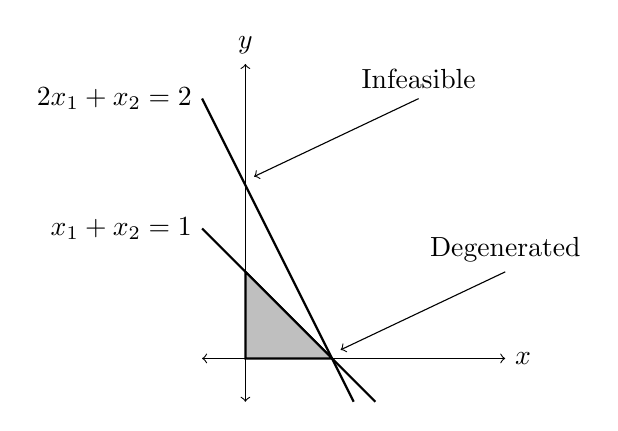
\begin{tikzpicture}[scale=1.1]

  \coordinate (a1) at (1.5, -0.5);
  \coordinate (a2) at (-0.5, 1.5);

  \coordinate (b1) at (1.25, -0.5);
  \coordinate (b2) at (-0.5, 3.0);

  \coordinate (orig) at (0,0);
  \coordinate (right) at (5,0);
  \coordinate (up) at (0,5);


  \draw[thick] (a1) -- (a2)node[left]{$x_1 + x_2 = 1$}; % a
  \draw[thick] (b1) -- (b2)node[left]{$2x_1 + x_2 = 2$}; % b

  \draw[<->] (-0.5,0) -- (3,0) node[right] {$x$};
  \draw[<->] (0,-0.5) -- (0,3.4) node[above] {$y$};

  \coordinate (ax) at (intersection of orig--right and a1--a2);
  \coordinate (ay) at (intersection of orig--up and a1--a2);

  \draw[thick,fill=lightgray] (orig) -- (ax) -- (ay) --cycle;

  \coordinate (tdeg) at (3,1);
  \draw[<-] (1.1,0.1) -- (tdeg) node[above] {Degenerated};

  \coordinate (tunf) at (2,3);
  \draw[<-] (0.1,2.1) -- (tunf) node[above] {Infeasible};
%    \foreach \i in {-2,...,7} {
%        \draw (\i,-0.1) -- (\i,0.1); 
%    }
%    \foreach \i in {-2,...,5} {
%        \draw (-0.1, \i) -- (0.1, \i);
%    }

%    \foreach \i in {-0,...,3} {
%       \foreach \j in {-0,...,3} {
%         \fill (\i,\j) circle (1.0pt);
%       }
%    }
  \end{tikzpicture}
\end{center}
\caption{\label{fig::basic_solutions}
Infeasible and degenerated basic solutions of 
(\ref{eq::degenerated_example}) to $\R^2$.}
\end{figure}


\begin{figure}[htb]
\begin{center}
  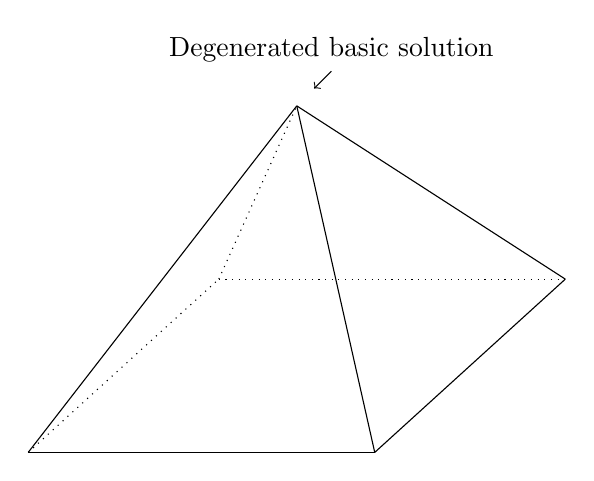
\begin{tikzpicture}[scale=1.1]

  \coordinate (a1) at (0.0, 0.0);
  \coordinate (a2) at (4.0, 0.0);

  \coordinate (a3) at (2.2, 2.0);
  \coordinate (a4) at (6.2, 2.0);

  \coordinate (c) at (3.1, 4.0);

%  \draw (a1) node {a1};
%  \draw (a2) node {a2};

%  \draw (a3) node {a3};
%  \draw (a4) node {a4};

%  \draw (c) node {c};

  \draw[-] (a1) -- (a2);
  \draw[-] (a2) -- (a4);

  \draw[dotted] (a1) -- (a3);
  \draw[dotted] (a3) -- (a4);

  \draw[-] (a1) -- (c);
  \draw[-] (a2) -- (c);
  \draw[dotted] (a3) -- (c);
  \draw[-] (a4) -- (c);

  \coordinate (c') at (3.3, 4.2);

  \draw[<-] (c') -- (3.5, 4.4) node[above] {Degenerated basic solution};

  \end{tikzpicture}
\end{center}
\caption{\label{fig::basic_solutions2}
A degenerated point in $\R^3$.}
\end{figure}





In this example we could easily make the degenerated basic solution
non-degenerated
by skipping the redundant constraint $2x_1 + x_2 \leq 2$. This is
always possible if we only have two non-slackness variables but 
already in three dimensions there are instances where we cannot
get rid of degenerated basic solutions.
As an example consider Figure~\ref{fig::basic_solutions2}. If the 
pyramid defines the set of all feasible solution the marked
vector is a degenerated basic solution, because four constraints are 
fulfilled with equality while there are only three non-slack variables.

Note that the example (\ref{eq::degenerated_example})
shows that the same vertex of a polyhedron can
belong to a degenerated or a non-degenerated basic solution, depending
on how we describe the polyhedron by a system of inequalities. 

%Vertex corresponds to feasible basic solution

\linebox{
\theorem{
Let $P=\{x \in \R^n \mid Ax=b, x\geq 0\}$ be a polyhedron
with $\mbox{rank}(A) = m < n$. Then a vector $x' \in P$ is a
vertex of $P$ if and only if it is a feasible basic solution.\\
}}


\prove 
%\ifdefined\OnlineVersion{}
%Exercise.
%\else
%``$\Rightarrow$:'' Let $x'$ be a vertex of $P$. Then, by 
%  Proposition~\ref{theorem::vertex}, $x'$ cannot be written as a 
%convex combination of vectors in $P \setminus\{x'\}$. 
%Assume that $x'$ is not a basic solution.
%Let $S = \{j \in \{1,\dots,n\} \mid x'_j > 0\}$.
%Then, the column vectors of $A_S$ are linearly dependent
%(otherwise we could extend
%$S$ to a basis, so $x'$ would be a basic solution).
%This means that there are numbers $(\lambda_j)_{j\in S}$ 
%such that not all of them are zero and such that
%$\sum_{j \in S} \lambda_j a_{ij} = 0$ for a $i \in \{1,\dots,m\}$
%(with $A = (a_{ij})_{{i=1,\dots,m}\atop{j=1,\dots,n}}$).
%For $j \in \{1,\dots,n\} \setminus S$, we set $\lambda_j = 0$,
%so we get a vector $\lambda = (\lambda_1,\dots,\lambda_n) \in \R^n$.
%For sufficiently small $\epsilon > 0$ we have $x' + \epsilon \lambda \in P$
%and $x' - \epsilon \lambda \in P$.
%Moreover, 
%$x' = \frac{1}{2}(( x' + \epsilon \lambda ) + ( x' - \epsilon \lambda  ))$
%which is a contradiction to the assumption that $x'$ is not the
%convex combination of vectors in $P \setminus\{x'\}$. 
%``$\Leftarrow$:'' 
The vector $x'$ is a vertex of $P$ if and only if it is a
%Let $x'$ be a feasible basic solution with basis $B$.
%This implies that $x'$ is a feasible solution of the following system
%of inequalities:
feasible solution of the following system and fulfills
$n$ linearly independent inequalities of the system with equality:
\[
   \begin{array}{rcl}
   Ax     & \leq & b\\
  -Ax     & \leq & -b\\
   -I_n x & \leq & 0
\end{array}
\]
This is the case if and only if $x'\geq 0$, 
$Ax' = b$ and $x'_{N} = 0$ for a set 
$N \subseteq \{1,\dots,n\}$ with $|N| = n - m$ such
that with $B = \{1,\dots,n\}\setminus N$ the 
matrix $A_B$ has full rank.
%it fulfills the $m$
%equations $Ax = b$ and has $n-m$ variables that are $0$,
%while the remaining variables are non-negative.
This is equivalent to being a feasible basic solution.
%where $I$ is the $n\times n$-identity matrix.
%Moreover, $x'$ fulfills $n$ linearly independent
%inequalities with equality (the $m$ inequalities in
%$Ax\leq b$ and $n - m$ of the last $n$ inequalities). 
%Hence, again by Proposition~\ref{theorem::vertex}, $x'$ 
%is a vertex.
%\fi %onlineversion
\endproof





\subsection{The Simplex Method}
\label{sec:simplex-tableau}
Before we describe the algorithm in general, we will present
some examples (which are taken from \cite{MatG07}).

%See Chapter 5 of \cite{MatG07}.

%Examples: standard, unbounded, degenerated, infeasible

Consider the following linear program:

\begin{equation*}
\begin{array}{rrcrccrcrcrl}
\max  &  x_1 & + &  x_2 &   &     &   &     &   &     &     &  \\
 s.t. & -x_1 & + &  x_2 & + & x_3 &   &     &   &     &  =  & 1\\
      &  x_1 &   &      &   &     & + & x_4 &   &     &  =  & 3\\
      &      &   &  x_2 &   &     &   &     & + & x_5 &  =  & 2\\
      &  x_1 & , &  x_2 & , & x_3 & , & x_4 & ,  & x_5 & \geq & 0
\end{array}
\end{equation*}

\[
\left(
\begin{array}{ccccc}
  -1 & 1 & 1 & 0 & 0\\
   1 & 0 & 0 & 1 & 0\\
   0 & 1 & 0 & 0 & 1\\
\end{array}
\right)
\left(
   \begin{array}{c}
       x_1\\
       x_2\\
       x_3\\
       x_4\\
       x_5
   \end{array}
\right)
= 
\left(
   \begin{array}{c}
       1\\
       3\\
       2\\
   \end{array}
\right)
\] 

We first need a basis to start with. We simply choose $B=\{3,4,5\}$, which gives us the
basic solution $x = (0,0,1,3,2)$.
We write the constraints and the objective function in a so-called 
{\hi simplex tableau}:

\[
\begin{array}{ccccccc}
x_3 & = & 1 & + & x_1 & - & x_2 \\
x_4 & = & 3 & - & x_1 &   &     \\
x_5 & = & 2 &   &     & - & x_2 \\ \hline
z   & = &   &   & x_1 & + & x_2 \\
\end{array}
\]

The first three rows describe an equation system that is equivalent
to the given one but each basic variable is written as a combination of
the non-basic variable. The last line describes the objective function.

We will try to increase non-basic variables (which are zero in the current 
solution) with a positive coefficient in the objective function.
Hence, here we could use $x_1$ or $x_2$, and we choose $x_2$.
%Increase the non-basic $x_2$.
Equation $x_3 = 1 + x_1 - x_2$ is the critical constraint that prevents us from
increasing to something bigger than 1 (without increasing $x_1$).
If we set $x_2$ to something bigger than 1, $x_3$ would become negative.
The constraint $x_5  = 2 - x_2$ only gives an upper bound of $2$ for the
value of $x_2$. Since the bound induced by non-negativity of $x_3$ is
tighter (so the constraint $x_3 = 1 + x_1 - x_2$ is critical),
we replace $3$ in the basis by $2$. The new 
basic variable $x_2$ can be written as a combination of the non-basic 
variables by using the first constraint:
$x_2 = 1 + x_1 - x_3$. The new base is $B = \{2,4,5\}$ with a new basic solution
$x = (0,1,0,3,1)$.
This is the new simplex tableau:
\[
\begin{array}{ccccccc}
x_2 & = & 1 & + &  x_1 & - & x_3 \\
x_4 & = & 3 & - &  x_1 &   &     \\
x_5 & = & 1 & - &  x_1 & + & x_3 \\ \hline
z   & = & 1 & + & 2x_1 & - & x_3 \\
\end{array}
\]

Increase $x_1$. $x_5 = 1 - x_1 + x_3$ is critical.
$x_1 = 1 + x_3 - x_5$.  New base $B = \{1,2,4\}$.
$x = (1,2,0,2,0)$.

\[
\begin{array}{ccccccc}
x_1 & = & 1 & + &  x_3 & - &  x_5 \\ 
x_2 & = & 2 &   &      & - &  x_5 \\
x_4 & = & 2 & - &  x_3 & + &  x_5 \\ \hline
z   & = & 3 & + &  x_3 & - & 2x_5 \\
\end{array}
\]

Increase $x_3$. $x_4 = 2 - x_3 + x_5$ is critical.
$x_3 = 2 - x_4 + x_5$. New base $B = \{1,2,3\}$.
$x = (3,2,2,0,0)$.

\[
\begin{array}{ccccccc}
x_1 & = & 3 & - &  x_4 &   &      \\ 
x_2 & = & 2 &   &      & - &  x_5 \\
x_3 & = & 2 & - &  x_4 & + &  x_5 \\ \hline
z   & = & 5 & - &  x_4 & - &  x_5 \\
\end{array}
\]

The value of the objective function for any
feasible solution $(x_1,\dots,x_5)$ is $5 - x_4 - x_5$.
Since we have found a solution where $x_4 = x_5 = 0$ 
and we have the constraint that $x_i \geq 0$ 
($i=1,\dots,5$), our solution is an optimum solution.



{\bf Unbounded instance:}

As a second example, consider:

\begin{equation*}
\begin{array}{rrcrccrcrl}
\max  &  x_1 &   &      &   &     &   &    &     &  \\
 s.t. &  x_1 & - &  x_2 & + & x_3 &   &     &  =  & 1\\
      & -x_1 & + &  x_2 &   &     & + & x_4 &  =  & 2\\
      &  x_1 & , &  x_2 & , & x_3 & , & x_4 & \geq & 0
\end{array}
\end{equation*}

Quite obviously this LP in unbounded (one can choose $x_1$ arbitrarily
large and set $x_2 = x_1$, $x_3 = 1$, and $x_4 = 2$).

Again we use the ``slack variables'' (here $x_3$ and $x_4$)
for a first basis. This gives $B=\{3,4\}$ and
$x = (0,0,1,2)$.

\[
\begin{array}{ccccccc}
x_3 & = & 1 & - & x_1 & + & x_2 \\
x_4 & = & 2 & + & x_1 & - & x_2 \\ \hline
z   & = &   &   & x_1 &   &     \\
\end{array}
\]

Increase $x_1$. $x_3 = 1 - x_1 + x_2$ is critical.
$x_1 = 1 + x_2 - x_3$.  New base $B = \{1,4\}$.
$x = (1,0,0,3)$.

\[
\begin{array}{ccccccc}
x_1 & = & 1 & + & x_2 & - & x_3 \\
x_4 & = & 3 &   &     & - & x_3 \\ \hline
z   & = & 1 & + & x_2 & - & x_3 \\
\end{array}
\]

We can increase $x_2$ as much as we want (provided that we increase 
$x_1$ by the same amount). Thus the simplex tableau show that the
linear program is unbounded.

{\bf Degeneracy:}

A final example shows what may happen if we get a degenerated basic solution.

\begin{equation*}
\begin{array}{rrcrccrcrl}
\max  &     &   &   x_2 &   &     &   &    &     &  \\
 s.t. & -x_1 & + &  x_2 & + & x_3 &   &     &  =  & 0\\
      &  x_1 &   &      &   &     & + & x_4 &  =  & 2\\
      &  x_1 & , &  x_2 & , & x_3 & , & x_4 & \geq & 0
\end{array}
\end{equation*}

Starting basis is  $B = \{3,4\}$, so $x =(0,0,0,2)$ which
is a degenerated solution.

\[
\begin{array}{ccccccc}
x_3 & = &   &   & x_1 & - & x_2 \\
x_4 & = & 2 & - & x_1 &   &     \\ \hline
z   & = &   &   &     &   & x_2 \\
\end{array}
\]

We want to increase $x_2$. $x_3 = x_1 - x_2$ is critical.
$x_2 = x_1 - x_3$.  We will replace $3$ by $2$ in the basis.
However, we cannot increase $x_2$.
New base $B = \{2,4\}$.
$x = (0,0,0,2)$.

\[
\begin{array}{ccccccc}
x_2 & = &   &   & x_1 & - & x_3 \\
x_4 & = & 2 & - & x_1 &   &     \\ \hline
z   & = &   &   & x_1 & - & x_3 \\
\end{array}
\]

Increase $x_1$. $x_4 = 2 - x_1$ is critical.
$x_1 = 2 - x_4$. New base $B=\{1,2\}$.
$x = (2,2,0,0)$.

\[
\begin{array}{ccccccc}
x_1 & = & 2 &   &     & - & x_4 \\ 
x_2 & = & 2 & - & x_3 & - & x_4 \\ \hline
z   & = & 2 & - & x_3 & - & x_4 \\
\end{array}
\]

Again, we have found an optimum solution because all coefficients
of the non-basic variables in the objective function 
$z = 2 - x_3 - x_4$ are negative.

After these three examples, we will now describe the simplex method in general.

%Simplex tableau:{\index{Simplex tableau}}
For a basis $B$, the 
{\hi simplex tableau}{\index{Simplex tableau}}
is a system $T(B)$ of $m+1$ linear equations
with variables $x_1,\dots,x_n$ and $z$ 
with this form
% that has the same set of
%solutions as the system $Ax=b$, $z=c^t b$
\begin{equation} \label{eq::simplextableau}
\begin{array}{lclcc}
x_B & = & p   & + & Q x_N\\ \hline
z   & = & z_0 & + &r^t x_N
\end{array}
\end{equation}
and the following properties:
\begin{itemize}
   \item $x_B$ is the vector of the basic variables, $N=\{1,\dots,n\}\setminus B$, and
         $x_N$ is the vector of the non-basic variables,
    \item $T(B)$ has the same set of solutions as the system $Ax=b$, 
         $z=c^t x$.
    \item $p$ is a vector of length $m$,
            $Q$ is an $m \times(n-m)$-matrix, $r$ is a vector of length ${n-m}$, and $z_0 \in \R$.
\end{itemize}

Note that the entries of $p$  are not necessarily numbered from $1$ to $m$ but that
$p$ uses $B$ as the set of indices (and for $r$, we have a corresponding statement).
In particular, the rows of $Q$ are indexed by $B$ and the columns by $N$. We denote
the entries of $Q$ by $q_{ij}$ (where $i \in B$ and $j \in N$).

\linebox{
\lemma{\label{theorem:: simplextableauexists}
For each basis $B$, there is a simplex tableau $T(B)$.\\
}
}

\prove 
Set
$p = A_B^{-1}b$, $Q = -A_B^{-1} A_N$, $r = c_N - (c_B^t A_B^{-1} A_N)^t$,
and $z_0 = c_B^t A_B^{-1} b$.

Then $x_B = A_B^{-1}b -A_B^{-1} A_N x_N$ which is equivalent
to $A_B x_B = b - A_N x_N$ and $A x = b$.

Moreover, $z = c_B^t A_B^{-1} b + (c_N^t - (c_B^t A_B^{-1} A_N)) x_N
= c_B^t A_B^{-1} (b - A_Nx_N) + c_N^t x_N = c_B^t A_B^{-1} A_B x_B + c_N^t x_N
= c_B^t x_B + c_N^t x_N = c^t x$ for any solution $x$ of $Ax = b$.
\endproof

{\bf Remark:} It is easy to check that there is only {\it one} simplex tableau for every
feasible basis $B$.
% See Matousek/Gaertner.



The cost function $z_0 + r^t x_N$ does not directly depend on the basic variables
but only on the non-basic variables. Their impact on the overall cost is given
be the vector $r=c_N - (c_B^t A_B^{-1} A_N)^t$. An entry of $r$ is called
the {\hi reduced cost}{\index{Reduced cost}} of its corresponding non-basic variable.

If all reduced costs are non-positive, we have already found an optimum solution:

\linebox{
\lemma{\label{theorem:: simplexopt}
Let $T(B)$ be a simplex tableau for a feasible basis $B$. If $r \leq 0$, then
the basic solution of $B$ is optimum. Moreover, $y=A_B^{-t}c_B$ is an optimal solution to the dual LP $\min b^t y$ s.t. $A^t y\ge c$\\
}
}
Here, $A_B^{-t}=(A_B^{-1})^t$.

\prove
Let $x$ be the basic solution of $B$. Since $x_N = 0$, we have $c^t x = z_0 (= c_B^t A_B^{-1} b)$.
If $x^*$ is any feasible solution with value $z^*= c^t x^*$, then
$x^*$ and $z^*$ are also a solution of $T(B)$, and we have
(because of $r \leq 0$ and $x^*_N \geq 0$)
$z^* = z_0 + r^t x^*_N \leq z_0 = c^t x$.

For the second part, consider the solution $y=A_B^{-t}c_B$. We show that it is feasible to $A^t y\ge c$ and satisfies complementary slackness. The constraints can be partitioned as $A_B^t y\ge c_B$ and $A_N^t y\ge c_N$. By the definition of $y$, we have  $A_B^t y= c_B$. By the definition of $r=c_N-(c_B^t A_B^{-1}A_N)^t=c_N-A_N^t A_B^{-t}c_B=c_N-A_N^t y$, and the requirement $r\le 0$, we have that $A_N^t y\ge c_N$. 
Moreover, complementary slackness  (Theorem~\ref{theorem::ComplementaySlackness}) adapted to this form asserts that whenever $x$ and $y$ are primal and dual feasible, and $A^t_i y=c_i$ whenever $x_i>0$, then both of them are optimal. Since every $i$ for which $x_i>0$ is contained in $B$, and $A_B^t y= c_B$, it follows that $x$ and $y$ satisfy complementary slackness.
\endproof


\linebox{
\lemma{\label{theorem:: simplexunbounded}
Let $T(B)$ be a simplex tableau for a feasible basis $B$. 
If there is an $\alpha \in N$ with
$r_\alpha > 0$ such that the column of $Q$ with
index $\alpha$ contains 
non-negative entries only, the 
linear program is unbounded.\\
}
}

\prove 
Let $x$ the feasible basic solution for $B$. Let $K \in \R$ 
with $K > c^t x$ be a constant.
Define a new feasible solution $\tilde x$ as follows: 
$\tilde x_\alpha := \frac{K - c^tx}{r_\alpha}$, 
$\tilde x_i = x_i$ for $i \in N \setminus \{ \alpha \}$, and
$\tilde x_j := p_j + q_{j \alpha} \tilde x_\alpha$ for
$j \in B$.
It is easy to check that $\tilde x$ is a feasible solution with
$c^t \tilde x \geq K$. Hence, the linear program is unbounded.
\endproof


In the following, we denote the entries of $A$ by $a_{ij}$ 
($i \in \{1,\dots,m\}$, $j \in \{1,\dots,n\}$). The column of $A$
with index $j$ is denoted by $a_{\cdot j}$.

\linebox{
\lemma{\label{theorem:: simplexnewbase}
Let $T(B)$ be a simplex tableau for a feasible basis $B$. 
Let $\alpha \in N$ be an index with $r_\alpha > 0$ and 
$\beta \in B$ with $q_{\beta \alpha} < 0$ and
$\frac{p_{\beta}}{q_{\beta \alpha}} = \max\{\frac{p_i}{q_{i \alpha}}\mid q_{i \alpha} < 0, i \in B \}$.
Then 
$\tilde B = (B \cup \{\alpha\}) \setminus \{\beta\}$ is a feasible basis.\\
}
}

\prove We have to show that $A_{\tilde B}$ has full rank and that it is feasible
i.e.\ that its basic solution is non-negative.
\begin{itemize}
   \item[(i)] $\tilde B$ is a basis:
       We will show that $A_B^{-1} A_{\tilde B}$ has full rank.

       All but one columns of $A_{\tilde B}$ belong to $A_B$. Hence, the matrix
       $A_B^{-1} A_{\tilde B}$ contains all unit vectors $e_i$ with the possible
       exception of $e_\beta$ because we removed the $\beta$-th column from $A_B$.
       However, this removed column has been replaced by
       the $\alpha$-th column $a_{\cdot \alpha}$ of $A$, so the remaining column of
       $A_B^{-1} A_{\tilde B}$ is $A_B^{-1} a_{\cdot \alpha}$. But this is exactly the 
       column with index $\alpha$ of $-Q = A_B^{-1} A_N$. By construction, $q_{\beta \alpha} \neq 0$,
       so all columns of $A_B^{-1} A_{\tilde B}$ are linearly independent.
   \item[(ii)] We have to show that the basic solution of $\tilde B$ is non-negative.
       We increase $x_\alpha$ to $-\frac{p_\beta}{q_{\beta \alpha}}$
       and set the basic variables $x_B$ to $p - q_{\cdot \alpha} \frac{p_\beta}{q_{\beta \alpha}}$,
       where $q_{\cdot \alpha}$ is the column with index $\alpha$ of $Q$.
       For $i \in B$ with $q_{i \alpha} \geq 0$ (so in particular $i \neq \beta$)
       we have $p_i - q_{i \alpha}  \frac{p_\beta}{q_{\beta \alpha}} \geq p_i \geq 0$.
       For $i \in B$ with $q_{i \alpha} < 0$ we have 
       $\frac{p_\beta}{q_{\beta \alpha}} \geq \frac{p_i}{q_{i \alpha}}$, so 
       $p_i \geq q_{i \alpha} \frac{p_\beta}{q_{\beta \alpha}}$ with equality in the last
       inequality for $i = \beta$.
       This leads to $x_\beta = 0$ and $x_B \geq 0$, so we 
       get a feasible basic solution for $\tilde B$.  \endproof
\end{itemize}
 

%Proof that optimality and unboundedness can be checked using the simplex tableau



\begin{algorithm}[htb]{\index{Simplex Algorithm@{\sc Simplex Algorithm}}}
\SetNlSty{textbf}{\hspace{1.5em}}{}%
\DontPrintSemicolon
\SetFuncSty{textsf}
\SetKw{KwGoTo}{go to}
\KwIn{A matrix $A\in\R^{m \times n}$, a vector $b \in \R^m$, and a vector $c \in \R^n$}
 \KwOut{A vector $\tilde x \in \{x \in \R^n \mid Ax=b, x\geq 0\}$ maximizing $c^t x$
 or the message that 
$\max\{c^t x \mid Ax=b, x\geq 0\}$ is unbounded or infeasible
}
  Compute a feasible basis $B$; \label{algo:init}\ifdefined\OnlineVersion{}\else\linebreak
  \comm{// See the Remark after Lemma~\ref{theorem:: simplexnewbase}.}\fi\;
  If no such basis exists, stop with the message ``{\sc infeasible}'';\;
  Set $N = \{1,\dots,n\}\setminus B$ 
    and compute the feasible basic solution $x$ for $B$;\linebreak
  \label{algo:beg_iteration}
\comm{// $x_B = A_B^{-1} b$, $x_N = 0$.}\;
  Compute the simplex tableau T(B)
\[
\begin{array}{lclcc}
x_B & = & p   & + & Q x_N\\ \hline
z   & = & z_0 & + &r^t x_N 
\end{array}
\]
  for the basis $B$;\quad
\comm{// See equation (\ref{eq::simplextableau}) and the following notation.}\;
  \If{$r \leq 0$} {\nonl \Return $\tilde x = x$; \quad
\comm{// $\tilde x$ is optimum (see Lemma~\ref{theorem:: simplexopt}).}}
  Choose an index $\alpha \in N$ with $r_{\alpha} > 0$;\label{algo:piv1} \linebreak
\comm{// Here we can apply different pivot rules.}\;
  \If{$q_{i \alpha} \geq 0$ for all $i\in B$}
  {\nonl \Return ``{\sc unbounded}''; \quad
\comm{// By Lemma~\ref{theorem:: simplexunbounded}, the LP is unbounded.}}
  Choose an index $\beta \in B$ with $q_{\beta \alpha} < 0$ and
  $\frac{p_{\beta}}{q_{\beta \alpha}} = \max\{\frac{p_i}{q_{i \alpha}}\mid q_{i \alpha} < 0, i \in B \}$;
    \label{algo:piv2}\linebreak
\comm{// Again, we can apply different pivot rules.}\;
  Set $B = (B\setminus\{\beta\}) \cup \{\alpha\}$;\linebreak
\comm{// See %equation~(\ref{eq::sigma}) for the notation and 
Lemma~\ref{theorem:: simplexnewbase} proving that we get a new feasible basis.}\;
 \KwGoTo line~\ref{algo:beg_iteration}\;
% initialization\;
% \While{not at end of this document}{
%  read current\;
%  \eIf{understand}{
%   go to next section\;
%   current section becomes this one\;
%   }{
%   go back to the beginning of current section\;
%  }
% }
 \caption{Simplex Algorithm}\label{alg::simplex}
\end{algorithm}

%General description
Algorithm~\ref{alg::simplex} summarizes the {\sc Simplex Algorithm}.



{\bf Remark:} In line~\ref{algo:init} of the algorithm we have to compute an 
initial feasible basis. This can be done with the following trick: 
We assume that the {\sc Simplex Algorithm} works correctly and has a finite
running time, provided that we can compute an initial basis.
We further assume that $b\geq 0$ (otherwise, we have to multiply some 
equations by -1 first).
Then, we set $\tilde A = \left(A \mid I_m\right)$, %(where $I$ is 
%the $m\times m$ identity matrix), 
add new variables 
$x_{n+1},\dots,x_{n+m}$, and solve (with $\tilde x = (x_1,\dots,x_{n+m})$)
the following problem:

\begin{equation}
\begin{array}{rl}
\max & -(x_{n+1} + x_{n+2} + \dots + x_{n+m}) \\
 \mbox{s.t.} & \tilde A \tilde x = b\\
 & \tilde x \geq 0
\end{array}
\end{equation}
For this linear program, it is trivial to find a feasible basis 
(${\{n+1,\dots,n+m\}}$ will work), so we can solve it by
the {\sc Simplex Algorithm}. If the value of its optimum solution
is negative, this means that the original linear program does not
have a feasible solution. Otherwise, the {\sc Simplex Algorithm}
will provide a basic solution for the original linear program.
In this case, the solution of the new LP computed by the
{\sc Simplex Algorithm} could contain variables from $x_{n+1},\dots,x_{n+m}$
as basic variables but their value must be $0$ and hence they can be
replaced easily by variables from $x_1,\dots,x_n$.


In lines~\ref{algo:piv1} and \ref{algo:piv2}, we may have a choice between
different candidates to enter or leave the basis. The elements chosen
in these steps are called pivot elements, and the rules by which we choose
them are called {\hi pivot rules}{\index{Pivot rule}}. Several different 
pivot rules for the entering variable have been proposed:
\begin{itemize}
   \item {\hi Largest coefficient rule}:{\index{Largest coefficient rule}}
       For the entering variable choose
       $\alpha$ such that $r_\alpha$ is maximized. This is the rule 
       that was proposed by Dantzig in his first description of the 
       {\sc Simplex Algorithm}.
   \item {\hi Largest increase rule}:{\index{Largest increase rule}}
       Choose the entering variable such
       that the increase of the objective function is maximized. Finding
       an $\alpha$ with that property takes more time because it is not  
       sufficient to consider the vector $r$ only.
   \item {\hi Steepest edge rule:}{\index{Steepest edge rule}}
       Choose the entering 
       variable in such a way that we move the feasible basic solution
       in a direction as close to the direction of the vector $c$ as possible.
       This means we maximize 
       \[
         \frac{c^t(x_{\scriptsize{new}} - x_{\scriptsize{old}}) }
              {|| x_{\scriptsize{new}} - x_{\scriptsize{old}} || }
       \]
       where $x_{\scriptsize{old}}$ is the basic feasible solution of the
       current basis and $x_{\scriptsize{new}}$ is the basic feasible solution
       of the basis after the exchange step. This rule is even more 
       timing-consuming but in many practical experiments it turned out
       to lead to a small number of exchange steps.
\end{itemize}



Here, we only analyze a pivot rule that is quite inefficient in practice but has
the nice property that we can show that the {\sc Simplex Algorithm} terminates
at all, if we follow that rule.
If all exchange steps improve the value of the current solution, we can be
sure that the algorithm will terminate because we can never visit the same
basic solution twice, and there is only a finite (though exponential) number
of basic solutions. 
However, exchange steps do not necessarily change the value of the solution.
Therefore, depending on the pivot rules, it is possible that the
{\sc Simplex Algorithm} runs in an endless loop by considering the same
sequence of bases forever. This behavior is called
{\hi cycling}{\index{Cycling}} (see page 30 ff.\ of \cite{Chv83} for an example
that this can really happen). The good news is that we can avoid cycling
by using an appropriate pivot rule.

%Hovewer, in cases of degenerated basic solutions, there can 
%be several bases for the same basic solution, and we have to avoid that the
%algorithm only runs exchange steps where it computes different bases for the
%the same basic solution. This possible behavior of the algorithm is called
%{\hi cycling}{\index{Cycling}} (see page 30 ff.\ of \cite{Chv83} for an example
%that this can really happen). The good news is that we can avoid cycling
%by using an appropriate pivot rule.


If the algorithm does not terminate, it has to consider the same basis 
$B$ twice. The computation between two occurrences of $B$
is called a cycle.
Let $F \subseteq\{1,\dots,n\}$ be the indices of the variables that have been
added to (and hence removed from) the basis during one cycle.
We call $x_F$ the cycle variables.


\linebox{
\lemma{
If the {\sc Simplex Algorithm} cycles, all basic solutions during the
cycling are the same and all cycle variables are $0$.\\
}
}

\prove 
The value of a solution considered in {\sc Simplex Algorithm} never 
decreases, so during cycling it cannot increase either.
Let $B$ be a feasible basis that occurs in the cycle, and let 
$B' = (B \cup \{\alpha\}) \setminus \{\beta\}$ be the next basis.
The only non-basic variable that could be increased is $x_\alpha$.
However, if it indeed was increased, then, because $r_\alpha > 0$,
this would increase the value of the solution. This shows that
the non-basic variables remain zero. But then, all variables
remain unchanged because the basic variables are determined uniquely
by the non-basic variables.
\endproof


A pivot rule that is able to avoid cycling is 
{\hi Bland's rule}{\index{Bland's rule}} (\cite{Bla77})
that can be described as follows:
In line~\ref{algo:piv1} of the {\sc Simplex Algorithm},
we choose $\alpha$ among all elements in
$N$ with $r_\alpha > 0$ such that $\alpha$
is minimal. In line~\ref{algo:piv2}, we choose $\beta$ among all elements
in $B$ with $q_{\beta \alpha} < 0$ and
 $\frac{p_{\beta}}{q_{\beta \alpha}} = \max\{\frac{p_i}{q_{i \alpha}}\mid q_{i \alpha} < 0, i \in B \}$
such that $\beta$ is minimal.


\linebox{
\theorem{
With Bland's rule as pivot rule in lines~\ref{algo:piv1} and \ref{algo:piv2},
the {\sc Simplex Algorithm} terminates after a finite number of steps.\\
}
}

\prove
Assume that the algorithm cycles while using Bland's rule.
We use the notation from above and consider the set $F$ of
the indices of the cycle variables. Let $\pi$ be the largest element
of $F$, and let $B$ be the basis just before $\pi$ enters the basis. 
Let $p$,$Q$,$r$ and $z_0$ be the entries of the simplex tableau $T(B)$.
Let $B'$ be the basis just before $\pi$ leaves it. %, and let $\rho \in F$
%be the index that replaces $\pi$.
Let $p'$,$Q'$,$r'$ and $z_0'$ be the entries of the simplex tableau $T(B')$.

Let $N = \{1,\dots,n\} \setminus B$ be the set of the 
non-basic variables (so in particular $\pi \in N$). %We write 
%$N=\{l_1,\dots,l_{n-m}\}$ with $l_1 < \dots < l_{n-m}$.
%Let $\alpha \in \{1,\dots,n-m\}$ be the index with $l_\alpha = \pi$.
According to Bland's rule we
choose the smallest index and $\pi = \max(F)$, so when $B$ is considered,
$\pi$ is the only candidate in $F$ to enter the basis. In other words:
\begin{equation}\label{eq::bland1}
    r_\pi > 0 \mbox{ and }r_j \leq 0 \mbox{ for all } j \in N \cap (F\setminus\{\pi\}).
\end{equation}

%We write $B'=\{k'_1,\dots,k'_{m}\}$ with $k'_1 < \dots < k'_{m}$.
%Let $\beta'$ be the index of the leaving variable $\pi$, so $k'_{\beta'} = \pi$.
%(and $\pi = \sigma(B', \beta')$). 
Let $\alpha$ be the index 
entering $B'$.
%, so $\sigma(N', \alpha) = \rho$:
Again by Bland's rule, 
$\pi$ must have been the only
candidate among all elements of $F$ to leave $B'$. Since $p'_j=0$ for
all $j \in B' \cap F$, %with %$k'_i \in F$
this means that
\begin{equation}\label{eq::bland2}
q'_{\pi \alpha} < 0 \mbox{ and }q'_{j \alpha} \geq 0 \mbox{ for } j \in B' \cap (F\setminus\{\pi\}).
% \mbox{ with }k'_i \in F.
\end{equation}

Roughly spoken, we will get a contradiction because~(\ref{eq::bland1}) says
that in a feasible basic solution
increasing a non-basic variable in $x_{F\setminus\{\pi\}}$ or decreasing
$x_\pi$ (to something negative!) will not improve the result. On the other hand,
(\ref{eq::bland2}) says that increasing $x_{\alpha}$ while decreasing 
$x_\pi$ (again to something negative) will improve the result.


We will formalize this statement by considering the following auxiliary linear program:
\begin{equation} \label{eq::auxLP}
   \begin{array}{rrcl}
   \mbox{max}   & c^tx                  &   & \\
   \mbox{s.t.\ } & Ax                    & =    & b\\
                & x_{F\setminus\{\pi\}} & \geq & 0\\
                & x_\pi             & \leq & 0\\
                & x_{N\setminus F}    &  = & 0
   \end{array}
\end{equation}
Note that there a no constraints on the signs of the variables
in $x_{B\setminus F}$.

We will show two claims that obviously cause a contradiction:

Claim 1: The LP~(\ref{eq::auxLP}) has an optimum solution.

Proof of Claim 1: Let $\tilde x$ be a basic feasible solution (of the original LP)
of the basis $B$. We have $\tilde x_F = 0$, so in particular $\tilde x_\pi = 0$, and hence
$\tilde x$ is a feasible solution of~(\ref{eq::auxLP}).
The cost of any solution $x$ of $Ax=b$ can be written as $c^t x = z_0 + r^t x_N$.
For any solution $x$ of ~(\ref{eq::auxLP}), we have
\[
   x_{j}    \left\{ \begin{array}{ll}
                              \geq 0 & \mbox{ if } j \in F \setminus\{\pi\}\\
                              \leq 0 & \mbox{ if } j = \pi
                  \end{array}
          \right.
\]
Therefore, by statement (\ref{eq::bland1}),
$r_j x_{j} \leq 0$ for all $j \in n \cap F$.
With the condition $x_{N \setminus F}=0$ this leads to $r^t x_N\leq 0$ for any
solution $x$ of ~(\ref{eq::auxLP}). Therefore, the value of any such solution
is at most $z_0$, and 
thus $\tilde x$ is an optimum solution of~(\ref{eq::auxLP}). This proves Claim 1.

Claim 2: The LP~(\ref{eq::auxLP}) is unbounded.

The bases are changed during the cycling but we always have the same basic solution.
Hence, if $\tilde x$ is a feasible basic solution of the original LP for basis $B$
is also a feasible basic solution for
the basis $B'$. We choose a positive number $K$ and set 
$x_{\alpha}' = K$. For $j \in N' \setminus \{\alpha\}$ (with 
$N' = \{1,\dots,n\}\setminus B'$), we set $x_j' = \tilde x_j = 0$.
Moreover, we set $x_{B'} = p' + Q' x_{N'}'$. 
By~(\ref{eq::bland2}), this defines a feasible solution of the auxiliary
LP~(\ref{eq::auxLP}).
Since $\alpha$ was a candidate for entering the basis $B'$, we have $r_{\alpha}' > 0$.
Hence, we get a solution with value $c^t x' = z_0' + r'^t x_{N'}' = z_0' + K \cdot r_{\alpha}'$.
As we can choose $K$ arbitrarily large, this shows that LP~(\ref{eq::auxLP}) is unbounded.
\endproof


\subsection{Efficiency of the Simplex Algorithm}

We have seen that Bland's rule guarantees that the 
{\sc Simplex Algorithm} will terminate. What can we say about the
running time?
Consider for some $\epsilon$ with $0 < \epsilon < \frac{1}{2}$
the following example:
\begin{eqnarray*}
\max x_n & & \\
-x_1 & \leq & 0\\
x_1  & \leq & 1\\
 \epsilon x_{j-1} - x_j & \leq & 0 \quad\text{ for }j\in\{2,\dots,n\}\\
 \epsilon x_{j-1} + x_j & \leq & 1 \quad\text{ for }j\in\{2,\dots,n\}\\
\end{eqnarray*}
Of course, adding non-negativity constraints for all variables would not
change the problem. The polyhedron defined by these inequalities is called
{\hi Klee-Minty cube}{\index{Klee-Minty cube}}
(\cite{KleM72}). It turns out that the {\sc Simplex Algorithm}
with Bland's rule (depending on the initial solution)
may consider $2^n$ bases before finding the optimum solution. In 
particular, this example shows that we don't get a polynomial-time
algorithm.

The bad news is that for any of the above pivot rules instances
have been found where the {\sc Simplex Algorithm} with that particular
pivot rule has exponential running time (see e.g.\ \cite{GolS79} for the
steepest edge rule).

Assume that you are given an optimum pivot rule that guides you to an optimum
solution with a smallest possible number of iterations.
Then, the number of iterations depends on the following property of the instances:

%To get lower bounds for the number of iterations that the {\sc Simplex Algorithm}
%might perform (no matter which pivot rule you apply), the following
%definition could be useful:

\linebox{\definition{
The {\hi combinatorial diameter}{\index{Combinatorial diameter}}
of a pointed polyhedron $P$ is 
the diameter (i.e.\ the largest distance of two nodes)
of the undirected graph $G_P$, where 
$V(G_P)$ is the set of vertices of $P$ and two nodes $v,w \in V(G_P)$
are connected by an edge in $G_P$ if and only if there
is a face of dimension $1$ containing $v$ and $w$.\\ 
}}

Obviously, if we don't make any assumptions on the starting solution,
the number of iterations performed by the {\sc Simplex Algorithm} optimizing
over a polyhedron $P$ will be at least the combinatorial diameter of
$P$, even with an optimum pivot rule.

It is an open question what the largest combinatorial diameter of a $d$-dimensional
polyhedron with $n$ facets is. In 1957, W.\ Hirsch conjectured that the combinatorial
diameter could be at most $n-d$. This conjecture was open for decades but it has been
disproved by Santos \cite{San11} who showed that there is a $20$-dimensional 
polyhedron with $40$ facets and combinatorial diameter $21$.
More generally, he proved that there are counter-examples to the 
Hirsch conjecture with arbitrarily many facets.
Nevertheless, it is still possible that the combinatorial diameter is always
polynomially (or even linearly) bounded in the dimension and the number of facets.
An upper bound for the combinatorial diameter is $O(n^{2 + \log d })$,
which was proven by~\cite{KalK92}. 
This bound has been improved by~\cite{Tod14} to $O((n-d)^{\log d })$.
For an overview of this topic see Section~3.3 of \cite{Zie07}.



In practical experiments, the {\sc Simplex Algorithm} typically turns 
out to be very efficient.
It could also be proved that the average running time (with a
specified probabilistic model) is polynomial (see~\cite{Bor82}).
Moreover, \cite{SpiT05} have shown that the expected running time
on a slight perturbation of a worst-case instance can be bounded by
a polynomial (``smoothed analysis'', see also~\cite{DadH19})

\bigskip

{\bf Revised Simplex Algorithm}

If one implements the {\sc Simplex Algorithm} as described above, an
explicit computation of the simplex tableau can be time-consuming.
This can be avoided in the so-called 
{\sc Revised Simplex Algorithm}{\index{Revised Simplex Algorithm@{\sc Revised Simplex Algorithm}}}.
In particular, we do not have to store the $m \times (n-m)$-matrix $Q$ completely.
It is sufficient to compute the column of $Q$ with index $\alpha$
after we have found an $\alpha \in N$ with $r_\alpha > 0$. %This method
%is called {\hi column generation}{\index{Column generation}}.
Moreover, we do not really need the matrix $A_B^{-1}$. In fact, we only
want to solve equation system of the type $A_B y = d$. It is more efficient
to compute an LU-decomposition of $A_B$ and update it after each exchange step.







%In the definition of $p$, $Q$, $r$ and $z$, the inverse of the matrix 
%$A_B$ occurs. However, we do not have to compute $A_B^{-1}$ explicitely.
%In order to compute $p = A_B^{-1} b$ we simply have to solve the
%equation system $A_B p = B$. The same trick 


\subsection{Dual Simplex Algorithm}

If the linear program $\max\{ c^t x \mid Ax = b, x \geq0\}$ is feasible and
bounded then the {\sc Simplex Algorithm} does not only provide an optimum
primal solution but we can also get an optimum solution of the dual linear
program $\min\{ b^t y \mid A^t y \geq c\}$. To see this, let $B$ the 
feasible basis corresponding to the optimum computed by the {\sc Simplex Algorithm}.
Set $\tilde y = A_B^{-t} c_B$ (where $A_B^{-t} = (A_B^{t})^{-1}$).  This leads to 
$A_B^t \tilde y = c_B$ and $A_N^t \tilde y = A_N^t A_B^{-t} c_B \geq c_N$ where
the last inequality follows from the fact that in $T(B)$ we have
$0 \geq r = c_N - (c_B^t A_B^{-1} A_N)^t$. So the vector $\tilde y$ is feasible for
the dual LP, and it is an optimum solution because together with the
(primal) basic solution $\tilde x$ for the basis $B$, it satisfies the complementary
slackness condition $(\tilde y^t A - c^t) \tilde x = 0$.

In fact, the condition $r \leq 0$ in the simplex tableau $T(B)$ guarantees the 
existence of a dual solution $y$ with $y^t A_B = c_B^t$. 
In the {\sc Dual Simplex Algorithm}, we start with a feasible basic dual solution,
i.e.\ a feasible dual solution for which a basis $B$ exists with $y^t A_B = c_B^t$.
If $A_B^{-t} c_B$ is a feasible dual solution,
we call $B$ a {\em dual feasible basis}.\index{Dual feasible basis}
Then, we compute the corresponding simplex
tableau $T(B)$ (which exists for any basis not just a feasible basis).
Thus the vector $r$ will have no positive entry.
Note that $B$ may not be feasible, so entries of $p$ can be negative.
Now the algorithm swaps elements between the basis and the rest of the
variables similarly to the simplex algorithm but instead of keeping
$p$ non-negative it keeps $r$ non-positive.

For any basis $B$ such that in $T(B)$ the vector $r$ has no positive entry,
the following properties (that are easy to prove) are the basis of the
{\sc Dual Simplex Algorithm}:
\begin{itemize}
   \item There is a feasible dual solution $y$ with $y^t A_B = c_B$.
   \item If $p \geq 0$ then the current dual solution is optimum.
   \item $z_0$ is the current solution value of the dual solution.
   \item If there is a $\beta \in B$ with $p_\beta < 0$ such that
         $q_{\beta j} \leq 0$ for all $j \in N$, then the primal LP is
         infeasible.
   \item For $\beta \in B$ with $p_\beta < 0$ and $\alpha \in N$ with
         $q_{\beta \alpha} > 0$ with
         $\frac{r_\alpha}{q_{\beta \alpha}} \geq \frac{r_j}{q_{\beta j}}$ for all
         $j \in N$ with  $q_{\beta j} > 0$, then 
         $(B\setminus\{\beta\})\cup\{\alpha\}$ is a dual feasible basis.
         Then the value of the dual solution
         is changed by $\frac{-p_\beta}{q_{\beta \alpha}} r_\alpha$. In particular,
         if $r_\alpha \neq 0$ then the value of the dual solution gets smaller.
\end{itemize}

The {\sc Dual Simplex Algorithm}\index{Dual Simplex Algorithm@{\sc Dual Simplex Algorithm}}
simply applies the exchange steps in the 
last item until we get a feasible basis. The algorithm can be considered
as the  {\sc Simplex Algorithm} applied to the dual LP. Thus it can also
run into cycling and its efficiency is not better then the efficiency
of the {\sc Simplex Algorithm}.

However, in some applications, the {\sc Dual Simplex Algorithm} is very
useful: If you add an additional constraint to the primal LP, then a
primal solution can become infeasible, so in the {\sc Primal Simplex Algorithm}
we have to start from scratch. 
However, the dual solution is still feasible. It is possibly not optimal
but often it can be made optimal with just some iterations of the 
{\sc Dual Simplex Algorithm}.


\subsection{Network Simplex}

%\cite{Cun76};
%Chapter 9.6 from \cite{KorV18}; \cite{AhuMO93}; Chapter 7.3 from \cite{BerT97}

The {\sc Network Simplex Algorithm} can be seen as the {\sc Simplex Algorithm}
applied to {\sc Min-Cost-Flow-Problems}. Even for this special case, we cannot
prove a polynomial running time but it turns out that, in practice, 
the {\sc Network Simplex Algorithm} is among the fastest algorithms for 
{\sc Min-Cost-Flow-Problems}. Though it is a variant of the 
{\sc Simplex Algorithm}, it can be described as a pure combinatorial
algorithm.


\linebox{
\definition{
Let $G$ be an directed graph with capacities $u:E(G)\to \R_{>0}$ and 
numbers $b:V(G) \to \R$ with $\sum_{v \in V(G)} b(v) = 0$. A {\hi feasible 
$b$-flow in $(G,u,b)$} is a mapping $f:E(G) \to \R_{\geq 0}$ with
\begin{itemize}
\item $f(e) \leq u(e)$ for all $e \in E(G)$ and
\item $\sum_{e \in \delta^+_G(v)} f(e) - \sum_{e \in \delta^-_G(v)} f(e) = b(v)$ for all $v \in V(G)$.
\end{itemize}
{\index{b-flow@{$b$-flow}}}
}
}

{\bf Notation:} We call $b(v)$ the {\hi balance} of $v$. If $b(v) > 0$, we call it the
{\hi supply} of $v$, and if $b(v) < 0$, we call it the {\hi demand} of $v$. Nodes $v$
of $G$ with $b(v) > 0$ are called {\hi sources}, nodes $v$ with $b(v) < 0$ are called 
{\hi sinks}.

During this chapter, $n$ is always the number of nodes and $m$ the number
of edges of the graph $G$.


\problem{Minimum-Cost Flow Problem}
{A directed graph $G$, capacities $u:E(G)\to \R_{>0}$, numbers
$b:V(G) \to \R$ with $\sum_{v \in V(G)} b(v) = 0$, edge costs
$c:E(G) \to \R$.}
{Task:}{Find a $b$-flow $f$ minimizing $\sum_{e \in E(G)}c(e)\cdot f(e)$.}
{\index{Minimum-Cost Flow Problem@{\sc Minimum-Cost Flow Problem}}}

We will use the following standard notation:

\linebox{
\begin{definition}
Let $G$ be a directed graph. We define the graph
$\stackrel{\leftrightarrow}{G}$ by
$V(\stackrel{\leftrightarrow}{G}) = V(G)$ and 
$E(\stackrel{\leftrightarrow}{G}) = E(G) \dot \cup \{ \stackrel{\leftarrow}{e} \mid e \in E(G)\}$
where $\stackrel{\leftarrow}{e}$ is an edge from $w$ to $v$ if $e$ is an
edge from $v$ to $w$. $\stackrel{\leftarrow}{e}$ is called the
{\hi reverse edge} of $e$.
Note that $\stackrel{\leftrightarrow}{G}$ may have
parallel edges even if $G$ does not contain any parallel edges.
If we have edge costs $c : E(G) \to \R$ these are extended canonically
to edges in $E(\stackrel{\leftrightarrow}{G})$ by setting
$c(\stackrel{\leftarrow}{e}) = -c(e)$.

Let $(G,u,b,c)$ be an instance of the
{\sc Minimum-Cost Flow Problem} and
let $f$ be a $b$-flow in $(G,u)$. Then, the {\hi residual graph}{\index{Residual graph}} 
$G_{u,f}$ is defined
by $V(G_{u,f}) := V(G)$ and $E(G_{u,f}) := \{e \in E(G) \mid f(e) < u(e)\} \dot \cup
\{\stackrel{\leftarrow}{e} \in E(\stackrel{\leftrightarrow}{G}) \mid f(e) > 0\}$.
For $e \in E(G)$ we define the {\hi residual capacity}{\index{Residual capacity}}
of $e$ by
$u_f(e) = u(e) - f(e)$ and the residual capacity of $\stackrel{\leftarrow}{e}$
by $u_f(\stackrel{\leftarrow}e) = f(e)$.
\end{definition}
}

The residual graph contains the edges where flow can be increased as forward
edges and edges where flow can be reduced as reverse edges. In both cases,
the residual capacity is the maximum value by which the flow can be modified.
If $P$ is a subgraph of the residual graph, then an
{\hi augmentation}{\index{Augmentation of flow}} along
$P$ by $\gamma$ means that we increase the flow on forward edges in $P$ 
(i.e.\ edges in $E(G) \cap E(P)$) by $\gamma$ and reduce it on reverse edges
in $P$ by $\gamma$. Note that the resulting mapping is only
a flow if $\gamma$ is at most the minimum of the residual capacity of the edges
in $P$.



\linebox{
\definition{
Let $(G,u,b,c)$ be an instance of the {\sc Minimum-Cost Flow Problem}.
A $b$-flow $f$ in $(G,u)$ is called a {\hi spanning tree solution}{\index{Spanning tree solution}}
if the graph $(V(G), \{e \in E(G) \mid 0 < f(e) < u(e)\})$ does not contain
any undirected cycle.\\
}}

Spanning tree solutions can be interpreted as vertex solutions:

\linebox{
\lemma{\label{lemmma::tree_basis}
Let $(G,u,b,c)$ be an instance of the {\sc Minimum-Cost Flow Problem}.
A $b$-flow $f$ is a spanning tree solution if and only if
$\tilde x \in \R^{E(G)}$ with $\tilde x_e = f(e)$ is a vertex of the
polytope
\begin{equation}\label{eq::networkflowLP}
   \left\{x \in \R^{E(G)} \mid 0 \leq x_e \leq u(e) \,\,(e \in E(G)),
                   \!\!\!\sum_{e \in \delta^+(v)}\!\! x_e - \!\!\!\sum_{e \in \delta^-(v)}x_e = b(v) \,\1(v \in V(G))
   \right\}.
\end{equation}
}}

\prove
``$\Rightarrow$:''
Let $f$ be a spanning tree solution and $\tilde x \in \R^{E(G)}$ with $\tilde x_e = f(e)$
for $e \in E(G)$.
Consider all inequalities $x_e \geq 0$ for edges $e$ with $f(e) = 0$, 
$x_e \leq u(e)$ for edges $e$ with $f(e) = u(e)$
and for each connected component of $(V(G), \{e \in E(G) \mid 0 < f(e) < u(e)\})$
for all but one vertex the equation $\sum_{e \in \delta^+(v)} x_e - \sum_{e \in \delta^-(v)}x_e = b(v)$.
These are $|E(G)|$ linearly independent inequalities that are fulfilled with equality by
$\tilde x$. Hence $\tilde x$ is a vertex.

``$\Leftarrow$:''
Let $f$ be a $b$-flow. Assume that $\tilde x \in \R^{E(G)}$ with $\tilde x_e = f(e)$
is a vertex of the polytope~(\ref{eq::networkflowLP}).
Assume that $(V(G), \{e \in E(G) \mid 0 < f(e) < u(e)\})$
contains an undirected cycle $C$. Choose an $\epsilon > 0$ such that 
$\epsilon \leq \min\{ \min\{f(e), u(e) - f(e)\} \mid e \in E(C)\}$. 
Fix one of the two possible orientations of $C$. We call an edge of $C$ a
forward edge if its orientation is the same as the chosen orientation, otherwise
it is called backward edge. Set $x'_e = \epsilon$ for all forward edges and
$x'_e = -\epsilon$ for all backward edges. For all edges $e \in E(G) \setminus E(C)$,
we set $x'_e = 0$. Then $\tilde x + x'$ and $\tilde x - x'$ belong to the 
polytope~(\ref{eq::networkflowLP})
and $\tilde x = \frac{1}{2}((\tilde x + x') + (\tilde x - x'))$, so by
Proposition~\ref{theorem::vertex}, $\tilde x$ cannot be a vertex. Hence, we have a 
contradiction.
\endproof

\linebox{
\corollary{
Let $(G,u,b,c)$ be an instance of the {\sc Minimum-Cost Flow Problem}.
If there is a $b$-flow in $(G,u)$, then there is an optimum solution of
$(G,u,b,c)$ that is a spanning tree solution.\\
}
}

\prove
Since the polyhedron~(\ref{eq::networkflowLP}) is in fact a polytope, it is pointed,
so there is an optimum solution that is a vertex. Together with
Lemma~\ref{lemmma::tree_basis}, this proves the statement.
\endproof



\linebox{
\definition{
Let $(G,u,b,c)$ be an instance of the {\sc Minimum-Cost Flow Problem} where we
assume that $G$ is connected. A {\hi spanning tree structure}{\index{Spanning tree structure}}
is a quadruple $(r,T,L,U)$ where $r \in V(G)$, $E(G) = T \, \dot\cup \, L \, \dot\cup \, U$,
$|T| = |V(G)| - 1$, and $(V(G),T)$ does not contain any undirected cycle.\\
The {\hi $b$-flow $f$ associated to the spanning tree structure $(r,T,L,U)$} 
{\index{b-flow associated to a spanning tree structure@$b$-flow associated to a spanning tree structure}}
is defined by
\begin{itemize}
   \item $f(e) = 0$ for $e \in L$,
   \item $f(e) = u(e)$ for $e \in U$,
   \item $f(e) = \sum_{v \in C_e} b(v) + \sum_{e' \in U \cap \delta_G^{-}(C_e)}u(e') - 
        \sum_{e' \in U \cap \delta_G^{+}(C_e)}u(e')$ for $e \in T$ where we denote 
        by $C_e$ vertex set of the the connected component of $(V(G),T\setminus\{e\})$
        containing $v$ (for $e=(v,w)$).
\end{itemize}
Let $(r,T,L,U)$ be a spanning tree structure and $f$ the $b$-flow associated to it.
The structure $(r,T,L,U)$ is called {\hi feasible} 
{\index{Feasible spanning tree structure}}
if $0 \leq f(e) \leq u(e)$
for all $e \in T$.\\
An edge $(v,w)\in T$ is called {\hi downward} if $v$ is on the undirected $r$-$w$-path
in $T$, otherwise is is called {\hi upward}.\\

A feasible spanning tree structure $(r,T,L,U)$ is called {\hi strongly  feasible} 
{\index{Strongly feasible spanning tree structure}}
if $0 < f(e)$ for every downward edge $e \in T$ and $f(e) < u(e)$ for every upward
edge $e \in T$ (where $f$ is again the $b$-flow associated to $(r,T,L,U)$).

We call the unique function $\pi:V(G) \to \R$ with $\pi(r)=0$ and
$c_\pi(e) := c(e) + \pi(v) - \pi(w) = 0$ for all $e = (v,w) \in T$ the
{\hi potential associated to the spanning tree structure  $(r,T,L,U)$}.\\
{\index{Potential associated to a spanning tree structure}}
}
}

%\newpage

{\bf Remarks:}%\vspace*{-0.4cm}
\begin{itemize}
   \item Obviously, the $b$-flow associated to the spanning tree structure
        $(r,T,L,U)$ fulfills the flow conservation rule, but it may be infeasible.
   \item $\pi(v)$ is the length of the $r$-$v$-path in 
          $(\stackrel{\leftrightarrow}{G}, \stackrel{\leftrightarrow}{c})$ consisting 
         of edges of $T$ and their reverse edges, only.
   \item In a strongly  feasible tree structure, we can send a positive flow 
         from each vertex $v$ to $r$ along tree edges such that that the new flow 
         remains non-negative and fulfills the capacity constraints.
 \end{itemize}



\linebox{
\proposition{
Given an instance $(G,u,b,c)$ of the {\sc Minimum-Cost Flow Problem} and 
a spanning tree structure $(r,T,L,U)$, the $b$-flow $f$ and the potential $\pi$
associated to $(r,T,L,U)$
%can be computed in time $O(n)$ and the potential $\pi$ associated to $(r,T,L,U)$
can be computed in time $O(m)$.\\
}}

\prove
Since the potential $\pi$ just encodes the distances to $r$ in $T$,
a breadth-first search in the edges of $T$ and the reverse edges of $T$
is sufficient.

We can compute $f$ by scanning the vertices in an order of non-increasing
distance to $r$ in $T$.
\endproof

\linebox{
\proposition{\label{prop::network::optimal}
Let $(r,T,L,U)$ be a feasible spanning tree structure and $\pi$ the potential associated
to it. If $c_{\pi}(e) \geq 0$ for all $e \in L$ and $c_{\pi}(e) \leq 0$ for all $e \in U$,
then the $b$-flow associated to $(r,T,L,U)$ is optimum.\\
}
}

\prove
The flow associated to $(r,T,L,U)$ is a basic solution of the
standard linear programming formulation for the minimum-cost flow problem.
The criterion in the proposition is equivalent to the statement that
the reduced costs of all non-basic variables are non-positive. This
is equivalent to the optimality of the solution.
\endproof


For an edge $e=(v,w) \in E(\stackrel{\leftrightarrow}{G})\setminus T$ with
$\stackrel{\leftarrow}{e} \not \in T$, we call $e$ together 
with the $w$-$v$ path consisting of edges of $T$ and reverse edges of edges
of $T$ only, the {\hi fundamental circuit}{\index{Fundamental circuit}}
of $e$. The vertex closest to $r$ in the fundamental circuit is called
the {\hi peak}{\index{Peak}} of $e$.


Algorithm~\ref{alg::network_simplex} gives a summary of the 
{\sc Network Simplex Algorithm}. As an input, we need a
strongly feasible tree structure. However, even if there is a feasible
$b$-flow, such a strongly feasible tree structure may not exist.
But we can modify the instance such that we can easily find a 
strongly feasible tree structure $(r,T,L,U)$. We add artificial expensive
edges between $r$ and all other nodes. For each sink 
$v \in V(G) \setminus\{r\}$, we add an edge $(r,v)$ with $u((r,v)) = -b(v)$.
For all other nodes $v \in V(G)\setminus \{r\}$ we add an edges $(v,r)$ with
$u((v,r)) = b(v) + 1$. %Then, we set $f((r,v)) = -b(v)$ for all sinks $v$
%and set $f((v,r)) = b(v)$
Then, we get a strongly feasible spanning tree structure by setting $L$ to the
set of all old edges (i.e.\ without the artificial edges connecting $r$)
and by setting $U = \emptyset$. If the weight on the artificial edges
is high enough ($1 + n \max_{e \in E(G)}|c(e)|$ would be sufficient) and
there is a solution that does not use these edges at all, 
no optimum solution will send flow along these new edges, 
so the new instance is equivalent.


\begin{algorithm}[htb]{\index{Network Simplex Algorithm@{\sc Network Simplex Algorithm}}}
\SetNlSty{textbf}{\hspace{1.5em}}{}%
\DontPrintSemicolon
\SetFuncSty{textsf}
\SetKw{KwGoTo}{go to}
\KwIn{
   An instance $(G,u,b,c)$ of the {\sc Minimum-Cost Flow Problem} and
   a strongly feasible spanning tree structure $(r,T,L,U)$.
}
 \KwOut{
   A minimum-cost flow $f$.
}
Compute the $b$-flow $f$ and the potential $\pi$
   associated to $(r,T,L,U)$;\;

Let $e_0$ be an edge with $e_0 \in L$ and $c_\pi(e_0) < 0$ or
   an edge with $e_0 \in U$ and $c_\pi(e_0) > 0$;\;\label{alg::network::start_loop}

\If{\text{No such edge exists}}{\nonl \Return $f$}

Let $C$ be the fundamental circuit of $e_0$ (if $e_0 \in L$) or of
   $\stackrel{\leftarrow}{e_0}$ (if $e_0 \in U$) and let $\rho = c_\pi(e_0)$;\;

Let $\gamma = \min_{e' \in E(C)} u_f(e')$, and let $e'$ the last edge
where this minimum is attained when $C$ is traversed (starting at the
peak);\; \label{alg::network::line::gamma}

Let $e_1$ be the corresponding edge in the input graph, i.e.
$e' = e_1$ or $e' = \stackrel{\leftarrow}{e_1}$;\;

Remove $e_0$ from $L$ or $U$;\; \label{alg::network::line::modpi1}

Set $T = (T \cup \{e_0\}) \setminus \{e_1\}$;\;

\If{$e' = e_1$}{\nonl Set $U = U \cup\{e_1\}$;}
\Else{\nonl Set $L = L \cup\{e_1\}$;}

Augment $f$ along $\gamma$ by $C$;\;  

Let $X$ be the connected component of $(V(G), T\setminus\{e_0\})$ that contains $r$;\;

\If{$e_0 \in \delta^+(X)$}{\nonl Set $\pi(v) = \pi(v) + \rho$ for $v\in V(G)\setminus X$;}

\If{$e_0 \in \delta^-(X)$}{\nonl Set $\pi(v) = \pi(v) - \rho$ for $v\in V(G)\setminus X$; \label{alg::network::line::modpi2}}

\KwGoTo line~\ref{alg::network::start_loop};

\caption{Network Simplex Algorithm}\label{alg::network_simplex}
\end{algorithm}







\linebox{\theorem{
The {\sc Network Simplex Algorithm} terminates after a finite number of
iterations and computes an optimum solution.\\
}
}

\prove
It is easy to check that after the modification in the lines 
\ref{alg::network::line::modpi1} to \ref{alg::network::line::modpi2}
$f$ and $\pi$ are still the $b$-flow and the potential associated to
$(r,T,L,U)$.

We will show that the spanning tree structure $(r,T,L,U)$
remains strongly feasible. By the choice of $\gamma$ in 
line~\ref{alg::network::line::gamma} it remains feasible.

For an edge $e = (v,w)$ on $T$ let $\tilde e = (v,w)$ 
if $e$ is an upward edge and $\tilde e = (w,v)$ if $e$ is a
downward edge. We have to show that after an iteration of the 
algorithm, for all edges $e \in T$, the edge $\tilde e$ has
a positive residual capacity. This is obvious for all edges 
outside $C$. %Hence, let $e \in T$ be an edge such that $e$
%or $\stackrel{\leftarrow}{e}$ is in $C$. If $e$ 
For the edges on the path on $C$ from the head of $e'$ to the
peak of $C$, this is also obvious because we augment by
$\gamma = u_f(e')$ which is smaller than the residual capacities
on this path (by the choice of $e'$). For the remaining edges $e$
on $C - e'$, the residual capacity $u_f(\tilde e)$ is, after the augmentation, at least
$\gamma$. Thus, is if $\gamma > 0$, we are done.
But if $\gamma = 0$, then $e'$ must be on the path from the
peak to $e_0$, so for the edges $e$ on the path from the peak to
the tail of $e'$ we had $u_f(\tilde e) > 0$ before the augmentation
(because $(r,T,L,U)$ was strongly feasible), so this is still the
case after the augmentation.

We will show that we never consider the same spanning tree
structure twice. 
In each iteration, the cost of the flow is reduced by 
$\gamma|\rho|$, so if $\gamma > 0$, then we are done.
Hence assume that $\gamma = 0$.
Then $e_0 \neq e_1$ (since all capacities are positive).
Moreover, 
$e_0 \in L \cap \delta^-(X)$ or $e_0 \in U \cap \delta^+(X)$,
so $\sum_{v \in V(G)} \pi(v)$ will get larger (and it will never get
smaller).
% Thus, we assume
% in addition that $e_0 = e_1$. Then $X = V(G)$ and 
% $\sum_{v \in V(G)} \pi(v)$ remains unchanged. But then
% $|\{ e \in L \mid c_\pi(e) < 0 \}| + |\{ e \in U \mid c_\pi(e) > 0 \}|$
% is strictly decreased.
This shows that we can never get 
the same spanning tree structure twice.Since there is only
a finite number of spanning tree structures, this proves that
the algorithm will terminate after a finite number of iterations.

By Proposition~\ref{prop::network::optimal}, the output of the
algorithm is optimal when the algorithm terminates.
\endproof


\iffalse
%%%%%%%%%%%%%%%%%%%%%%%%%%%%%%%%%%%%%
\section{Sizes of Solutions}
%%%%%%%%%%%%%%%%%%%%%%%%%%%%%%%%%%%%%

Before we will describe polynomial-time algorithms for
solving linear programs we have to
make sure that we can store the output and all intermediate results
with numbers whose sizes are polynomial in the input size. To this
end we have to define the size of numbers. Assuming that all numbers
are given in a binary representation, we define for
\begin{itemize}
  \item $n \in \Z:$ $\size(n) := 1 + \lceil \log(|n|+1) \rceil$,
  \item $r = \frac{p}{q}$ with $p,q \in \Z$, relatively prime:
     $\size(r) := \size(p) + \size(q)$,
  \item vectors $x = (x_1,\dots,x_n)\in \Q^n$: $\size(x) := n + \sum_{i=1}^n \size(x_i)$,
  \item matrices $A= (a_{ij})_{{i=1,\dots,m}\atop{j=1,\dots,n}} \in \Q^{m\times n}$:
      $\size(A) := nm + \sum_{i=1}^m \sum_{j=1}^n \size(a_{ij})$.
\end{itemize}

{\bf Remark:} In order to get a description of a fraction $r$ of with
$\size(r)$ bits, we have to write $r$ as $\frac{p}{q}$ for numbers
$p,q \in \Z$ that are relatively prime. Therefore, in any computation,
when a fraction $\frac{p}{q}$ arises, we apply the Euclidean Algorithm
to $p$ and $q$ and divide $p$ and $q$ by their greatest common divisor.
The Euclidean Algorithm has polynomial running time, so during any
algorithm, we can assume that any fraction $r$ is stored by using just
$\size(r)$ bits.

\linebox{
\proposition{\label{theorem::prod_sum_small}
For $r_1,\dots,r_n \in \Q$, we have
\begin{itemize}
\item[(a)] $\text{size}\left(\prod\limits_{i=1}^n r_i\right) \leq \sum\limits_{i=1}^n\text{size}(r_i)$
\item[(b)] $\text{size}\left(\sum\limits_{i=1}^n r_i\right) \leq 2 \sum\limits_{i=1}^n\text{size}(r_i)$
\end{itemize}
}}


\prove
\ifdefined\InitialVersion{}
Exercise. \endproof
\else
Both statements are obvious if the numbers $r_1,\dots,r_n$ are integers.
Hence assume that $r_i = \frac{p_i}{q_i}$ for non-zero numbers 
$p_i$ and $q_i$ that are relatively prime ($i=1,\dots,n$).
\begin{itemize}
\item[(a)] $\text{size}\left(\prod\limits_{i=1}^n r_i\right) 
         \leq \text{size}\left(\prod\limits_{i=1}^np_i \right) + \text{size}\left(\prod\limits_{i=1}^n q_i \right)
         \leq \sum\limits_{i=1}^n \text{size}(p_i) + \sum\limits_{i=1}^n \text{size}(q_i)
           = \sum\limits_{i=1}^n \text{size}(r_i)$.
\item[(b)] We have\,\, $\text{size}\left(\prod\limits_{i=1}^n q_i\right) 
          \leq \sum\limits_{i=1}^n \text{size}(q_i)
          \leq \sum\limits_{i=1}^n \text{size}(r_i)$, and
         $\text{size}\left(\sum\limits_{i=1}^n p_i \prod\limits_{j\in\{1,\dots,n\} \setminus \{i\}}q_j \right)
         \leq \text{size}\left( \sum\limits_{i=1}^n |p_i| \prod\limits_{j=1}^n q_j \right)
         \leq \sum\limits_{i=1}^n\text{size}(r_i)$.
         Since $\sum\limits_{i=1}^n r_i = \frac{1}{\prod\limits_{i=1}^n q_i}
       \sum\limits_{i=1}^n p_i \prod\limits_{j\in\{1,\dots,n\} \setminus \{i\}}q_j$,
       this proves the claim. \endproof
\end{itemize}
\fi %Initialversion


\linebox{
\proposition{
For $x,y \in \Q^n$, we have
\begin{itemize}
\item[(a)] $\text{size}(x+y) \leq 2(\text{size}(x) + \text{size}(y))$
\item[(b)] $\text{size}(x^ty) \leq 2(\text{size}(x) + \text{size}(y))$
\end{itemize}
}}

\prove
\begin{itemize}
\item[(a)] We have {\small \[\text{size}(x+y) = n + \sum_{i=1}^n \text{size}(x_i + y_i)
                \leq n + 2\sum_{i=1}^n \text{size}(x_i) + 2\sum_{i=1}^n \text{size}(y_i)
                 = 2(\text{size}(x) + \text{size}(y)) -3n.\] }
\item[(b)]  We have 
\begin{eqnarray*} \text{size}(x^ty) & = & \text{size}\left(\sum_{i=1}^n x_iy_i\right) \leq 2\sum_{i=1}^n \text{size}(x_iy_i)
     \leq 2\left(\sum_{i=1}^n \text{size}(x_i) + \sum_{i=1}^n \text{size}(y_i)\right)\\
     & = & 2(\text{size}(x) + \text{size}(y)) -4n.
\end{eqnarray*} \endproof
\end{itemize}




\linebox{
\proposition{\label{theorem::det_small}
For any matrix $A \in \Q^{n\times n}$, we have
$\text{size}(\text{det}(A)) \leq 2 \text{size}(A)$.\\
}}


\prove
%\ifdefined\OnlineVersion{}
%Exercise. \endproof
%\else
Write the entries $a_{ij}$ of $A$ as $a_{ij} = \frac{p_{ij}}{q_{ij}}$
where $p_{ij}$ and $q_{ij}$ are relatively prime ($i,j=1,\dots,n$). 
Let $\text{det}(A) = \frac{p}{q}$ where $p$ and $q$ are relatively
prime, too.

Then $|\text{det}(A)| \leq \prod_{i=1}^{n}  \prod_{j=1}^{n} (|p_{ij}| + 1)$
and $|q| \leq \prod_{i=1}^{n}  \prod_{j=1}^{n} |q_{ij}|$. Therefore,
\[
   \text{size}(q) \leq \text{size}(A)
\]
and
$|p| = |\text{det}(A)||q| \leq \prod_{i=1}^{n}  \prod_{j=1}^{n} 
\Big((|p_{ij}| + 1) |q_{ij}| \Big)$. We can conclude
\[
   \text{size}(p) \leq \sum_{i=1}^n \sum_{j=1}^n (\text{size}(p_{ij}) + 1 + \text{size}(q_{ij})) 
    = \text{size}(A).
\]
This proves $\text{size}(\text{det}(A)) \leq 2 \text{size}(A)$.
\endproof
%\fi %onlineversion





\linebox{
\proposition{\label{theorem::SmallSolutions}
Let $\max\{c^t x \mid Ax\leq b\}$ be a feasible bounded
linear program with $A \in \Q^{m\times n}$ and $b \in \Q^m$. Then,
there is an optimum (rational) solution $x$ with 
$\size(x) \leq 4n(\size(A) + \size(b))$. If $b=e_i$ or $b=-e_i$ for
a unit vector $e_i$, then there is a non-singular submatrix $A'$ of
$A$ and an optimum solution $x$ with $\size(x) \leq 4n \size(A')$.\\
}
}

\prove
By Corollary~\ref{Corollary::faces} the maximum of $c^t x$ over 
$P = \{x \in \R^n \mid Ax \leq b\}$ must be attained in a minimal
face of $P$. Let $F$ be a minimal face where the maximum is attained.
By Proposition~\ref{proposition::minimal_faces}, we can write
$F= \{x \in \R^n \mid \tilde A x = \tilde b\}$  for some subsystem
$\tilde A x\leq \tilde b$ of $Ax \leq b$. We can assume that the
rows of $\tilde A$
are linearly independent. Choose $B \subseteq \{1,\dots,n\}$
such that $\tilde A_B$ is a regular square matrix.
 Then $x \in \R^n$ with
$x_B = {\tilde A_B}^{-1} \tilde b$ and $x_N = 0$ 
(with $N = \{1,\dots,n\}\setminus B$)
is an optimum solution of the linear program.
By Cramer's rule the entries of $x_B$ can be written as 
$x_j = \frac{\text{det}(\tilde A_j)}{\text{det}({\tilde A_B}) }$
where $\tilde A_j$ arises from $\tilde A_B$ by replacing the
$j$-th column by $\tilde b$. Thus, we have
$\text{size}(x) \leq n + 2n(\text{size}(\tilde A_j) + \text{size}(\tilde A_B))
\leq 4n(\text{size}(\tilde A_B) + \text{size}(\tilde b))$.

If $b \in \{e_i,-e_i\}$, then $|\text{det}(\tilde A_j)|$ is the
absolute value of a determinant of a submatrix of
$\tilde A_B$.
\endproof

\linebox{
\corollary{\label{corollary::minimal_solution_entries}
Let $\max\{c^t x \mid Ax\leq b\}$ be a feasible bounded
linear program with $A \in \Q^{m\times n}$ and $b \in \Q^m$. Then,
there is an optimum (rational) solution $x$ such that for each 
non-zero entry $x_j$ of $x$, we have 
$|x_j| \geq 2^{-4n(\size(A) + \size(b))}$.\\
%TODO: Lower bound for the size of a positive entry in the solution.
}
}

\prove
According to the proof of the previous proposition there is an optimum 
solution $x$ such that for each entry $x_j$ of $x$ we have
$\text{size}(x_j) \leq 4n(\size(A) + \size(b))$. Since every positive
number smaller than $2^{-4n(\size(A) + \size(b))}$ has a size larger than
$4n(\size(A) + \size(b))$, this proves the claim. 
\endproof




%\subsection{Continued Fractions}



\subsection{Gaussian Elimination}\label{sec::gauss}

Assume that we want solve an equation system $Ax = b$. We can 
do this by applying the Gaussian Elimination. {\index{Gaussian Elimination}}
This algorithm performs
three kinds of operations to the matrix $A$:
\begin{enumerate}
   \item Add a multiple of a row to another row.
   \item Swap two columns.
   \item Swap two rows.
\end{enumerate}
It should be well-known (see e.g.\ textbooks \cite{HouV18} or \cite{KorV18})
that with these steps $O(mn(\text{rank}(A) + 1))$ elementary 
arithmetical operations are sufficient to transform $A$ into 
an upper (right) triangular matrix. Then it is easy to check if the 
equation system is feasible, and, in case that it is feasible, to
compute a solution. However, in order to show that Gaussian Elimination
is a polynomial-time algorithm, we have to show that the numbers that
arise during the algorithm aren't too big.

The intermediate matrices that occur during the algorithm are of 
the type 
\begin{equation}
   \left(
      \begin{array}{cc}
          B & C \\
          0 & D 
      \end{array}
   \right),
\end{equation}
where $B$ is an upper triangular matrix.
Then, an elementary step of the Gaussian Elimination consist
of choosing a non-zero entry of $D$ (called pivot element;
if no such entry exists, we are done) 
and to swap rows and/or columns such that this element is at
position $(1,1)$ of $D$. Then we add a multiple of the 
first row of $D$ to the other rows of $D$ such that the
entry at position $(1,1)$ is the only non-zero entry of the
first column of $D$.

We want to prove that the numbers that occur during the algorithm
can be encoded using a polynomial number of bits. We can assume
that we don't need any swapping operation because swapping columns
or rows doesn't change the numbers in the matrix.


Assume that our current matrix is 
$\tilde A = \left(
      \begin{array}{cc}
          B & C \\
          0 & D 
      \end{array}
   \right)$ where $B$ is a $k \times k$-matrix.
%the current matrix is given by~(\ref{eq::gauss}).
%Denote the entries of $D$ by $d_{ij}$. 
Then for each entry $d_{ij}$ of $D$ we have
\begin{equation}\label{eq::gauss}
   \det(\tilde A^{1,\dots,k,k+i}_{1,\dots,k,k+j}) = d_{ij} \cdot \det(\tilde A^{1,\dots,k}_{1,\dots,k}).
%   d_{ij} = \frac{\det(\tilde A)^{1,\dots,k,k+i}_{1,\dots,k,k+j}}
%                {\det(\tilde A)^{1,\dots,k}_{1,\dots,k}}
\end{equation}
where $M^{i_1,\dots,i_t}_{j_1,\dots,j_t}$ denotes the submatrix of a matrix $M$
induced by the rows $i_1,\dots,i_t$ and the columns ${j_1,\dots,j_t}$.
To see the correctness of~(\ref{eq::gauss}), apply Laplace's formula
to the last row of $\tilde A^{1,\dots,k,k+i}_{1,\dots,k,k+j}$ which contains
$d_{ij}$ as the only non-zero element.
Since the 
determinant does not change if we add the multiple of 
a row to another row, this leads to
\begin{equation*}
d_{ij}  =  \frac{\det(A^{1,\dots,k,k+i}_{1,\dots,k,k+j})}
             {\det(A^{1,\dots,k}_{1,\dots,k})} 
\end{equation*}
By Proposition~\ref{theorem::det_small} and
Proposition~\ref{theorem::prod_sum_small},
this implies $\text{size}(d_{ij}) \leq 4 \, \text{size}(A)$. 
Since all entries of the matrix occur as entries of such a 
matrix $D$, this shows that the sizes of all numbers 
that are considered during the Gaussian Elimination
are bounded by $ 4 \text{size}(A)$. 

Note that we have to apply the 
Euclidean Algorithm to any intermediate result in order to 
get small representations of the numbers. But this is not a
problem because the Euclidean Algorithm is polynomial as well.

Finally, we get the result:

\linebox{
\proposition{
The Gaussian Elimination is an algorithm with polynomial running time.\endproof\\
}
}

In particular this result shows that the following problems can 
be solved with a polynomial running time:\vspace*{-3mm}
\begin{itemize}
   \item Solving a system of linear equations.
   \item Computing the determinant of a matrix.
   \item Computing the rank of a matrix.
   \item Computing the inverse of a regular matrix.
   \item Checking if a set of rational vectors is linearly independent.
\end{itemize}


\fi


%%%%%%%%%%%%%%%%%%%%%%%%%%%%%%%%%%
\section{Ellipsoid Method}
%%%%%%%%%%%%%%%%%%%%%%%%%%%%%%%%%%

The Ellipsoid Method (proposed by \cite{Kha79})
was the first polynomial-time algorithm for linear programming.
The algorithm solves the problem of finding a feasible
solution of a linear program. As we have seen in 
Section~\ref{sec::StrongDuality}, this is sufficient to solve
as well the optimization problem.



\subsection{Ellipsoid Method for Convex Feasibility}
We now present a general version of the ellipsoid method. This addresses the more general problem of finding a feasible point in a  compact convex set $K \subseteq \R^n$, given by a {\bf separation oracle}{\index{Separation oracle}}:
 For a convex set $K \subseteq \R^n$, a separation oracle is is a subroutine which, given $x \in \R^n$, either returns an $a \in \R^n$ with
$a^ty > a^tx$ for all $ y \in K$ or asserts $x \in K$.
For the ellipsoid algorithm, we can use an arbitrary `black-box' separation algorithm, as long as it provides these guarantees.

{\bf Observation:} Given $A \in \Q^{m \times n}$ and $b \in \Q^m$, a
separation oracle for $\{x \in \R^n \mid Ax \leq b\}$ can be implemented
in $O(mn)$ arithmetical operations.

In Section~\ref{sec:sizes}, we discuss how the general algorithm can be used to obtain a polynomial-time algorithm for linear programming. In the description below, the algorithm is allowed to take square-roots of numbers (of infinite precision). While this is not allowed in the Turing model of computation, a natural rounding of the algorithm can be used to avoid this, see Remark~\ref{rem:implementation}.


\linebox{
\definition{
A set $E \subset \R^n$ is an {\hi ellipsoid}{\index{Ellipsoid}}
if there are a vector 
$s\in\R^n$ and a nonsingular matrix $M\in \R^{n \times n}$ such that
\[
   E = \{Mx + s \mid x \in \B^n\}
\]
where $\B^n = \{x \in \R^n \mid x^tx \leq 1\}$ is the $n$-dimensional
unit ball.\\
}
}

As a short notation, we write $E = s + M \B^n$.

\linebox{
\definition{
A symmetric matrix $A$ is called {\hi positive definite}{\index{Positive definite matrix}}
if $x^t A x > 0$ for any non-zero vector $x$. It is called 
{\hi positive semidefinite}{\index{Positive semidefinite matrix}}
if $x^t A x \geq 0$ for any vector $x$.\\
}
}

{\bf Remark:}
An $n \times n$-matrix $Q$ is positive definite if and only
if there is a non-singular matrix $M$ such that $Q=MM^t$.
For example, the {\hi Cholesky decomposition}{\index{Cholesky decomposition}}
of $Q$ achieves this.
For a proof of this statement, we refer to textbooks
on linear algebra, e.g.\ \cite{Str80}.

\linebox{
\lemma{
A set $E \subset \R^n$ is an ellipsoid if and only if there is a (symmetric)
positive definite $n \times n$-matrix $Q$ and a vector $s \in \R^n$
such that $E = \{x \in \R^n \mid (x - s)^t Q^{-1} (x-s) \leq 1\}$.\\
}
}

\prove
A set $E \subseteq \R^n$ is an ellipsoid if and only if there
is a nonsingular matrix $M\in \R^{n \times n}$ and a vector 
$s \in \R^n$ such that
\[
   E = \{Mx + s \mid x \in B^n\} 
     = \{y \in \R^n \mid M^{-1}(y - s) \in \B^n\}
     = \{y \in \R^n \mid (y-s)^t(M^{-1})^t M^{-1}(y - s) \leq 1\}.
\]
But (using the previous remark)
this is equivalent to the statement that there is a
positive definite $n \times n$-matrix $Q$ and a vector $s \in \R^n$
such that $E = \{x \in \R^n \mid (x - s)^t Q^{-1} (x-s) \leq 1\}$.
\endproof






The {\sc Ellipsoid Algorithm}
just finds an element in an polytope or ends with the
assertion that the polytope is empty. On the other hand,
it can be applied to more general sets $K \subseteq \R^n$
provided that $K$ is a compact convex set and that for
any $x \in \R^n\setminus K$ we can find a half-space
containing $K$ such that $x$ is on the border of the half-space.

Basically, the algorithms works as follows: 
We always keep track of an ellipsoid containing $K$. 
Then we check if the center $c$ of the ellipsoid is 
contained in $K$. If this is the case, we are done.
Otherwise, we compute the intersection $X$ of the ellipsoid and
a half-space containing $K$ such that $c$ is on the border
of the half-space. Then, we find a new (smaller) ellipsoid
containing $X$.

For the 1-dimensional space, the ellipsoid method contains
the binary search as a special case. However, for technical
reasons, we assume in the following that the dimension of
our solution space is at least $2$.












We start with a special case that is easier to handle: 
We assume that our given
ellipsoid is the ball $B^n$ (with radius $1$ and center $0$).
We want to find a small ellipsoid $E$ covering the intersection of
$B^n$ with the half-space $\{x \in \R^n \mid x_1 \geq 0\}$ (the
gray area in Figure~\ref{fig::half-ball}).

\begin{figure}[htb]
\begin{center}
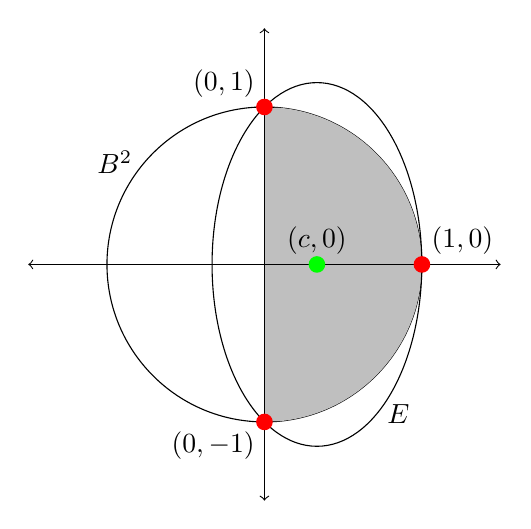
\begin{tikzpicture}[scale=2.0]
%\begin{scope}[rotate = 30]
%\draw[green] (2cm,-2cm) -- (-2cm,2cm);
%\clip[draw] (0,0) ellipse (2cm and 1cm);
%\draw[step=0.5cm, blue] (-2cm,-2cm) grid (2cm,2cm);
%\draw[red] (2cm,-2cm) -- (-2cm,2cm);
%\end{scope}
%\draw[line width=5pt] (-2cm,0) -- (2cm,0);
\begin{scope}
\clip[draw] (0,0) ellipse (1 and 1);
\draw[fill=lightgray] (0,-1) rectangle (1,1);
\end{scope}
\draw[<->] (-1.5, 0) -- (1.5, 0);
\draw[<->] (0, -1.5) -- (0, 1.5);
\draw (0.33333,0) ellipse (0.666 and 1.1547);
%\draw (0.33333,0) ellipse (0.866 and 1.5);
\fill[red] (1, 0) circle (1.5pt) node[above right, black]{$(1,0)$};
\fill[red] (0, 1) circle (1.5pt) node[above left, black]{$(0,1)$};
\fill[red] (0,-1) circle (1.5pt) node[below left, black]{$(0,-1)$};

\fill[green] (0.333333,0) circle (1.5pt) node[above, black]{$(c,0)$};
\draw (-0.95,  0.65) node{$B^2$};
\draw ( 0.85, -0.95) node{$E$};
\end{tikzpicture}
\end{center}
\caption{Intersection of $B^n$ with $\{x \in \R^n \mid x_1 \geq 0\}$.}
\label{fig::half-ball}
\end{figure}


For symmetry reasons, we choose the center of the new smaller ellipsoid on the
vector $e_1$ at a position $c \cdot e_1$ (where $c$ is still to be determined).
Our candidates for the ellipsoid are of the form 
\[
E=\left\{x \in \R^n \mid \alpha^2 (x_1 - c)^2 + \beta^2 \sum_{i=2}^n x_i^2 \leq 1\right\}
\]
where we also have to choose $\alpha$ and $\beta$. The matrix
$Q$ is then a diagonal matrix with entry $\frac{1}{\alpha^2}$ at 
position $(1,1)$ and $\frac{1}{\beta^2}$ on all other diagonal positions.


To keep $E$ small, we want $e_1$ to lie on the border of $E$.
This condition leads to $\alpha^2(1-c)^2=1$ and hence
\begin{equation}
\alpha^2 = \frac{1}{(1-c)^2}.
\end{equation}

Moreover, we want all points on the intersection of
the border of $B^n$ and $\{x\in \R^n \mid x_1 = 0 \}$ to be
on the border of  $E$. This condition leads to
$\alpha^2 c^2 + \beta^2 = 1$ and thus
\begin{equation}
  \beta^2 = 1 -\alpha^2 c^2 = 1- \frac{c^2}{(1-c)^2} = \frac{1-2c}{(1-c)^2}.
\end{equation}


The volume of an ellipsoid 
$E = \{x \in \R^n \mid (x - s)^t Q^{-1} (x-s) \leq 1\}$
is 
$\vol(E) = \sqrt{\det(Q)} \times \vol(B^n)$ (a result from measure
theory, see e.g.\ Proposition~6.1.2 in \cite{Coh80}).


Therefore, our goal is to choose $\alpha$, $\beta$ and $c$ in 
such a way that $\sqrt{\det(Q)} = \alpha^{-1}\beta^{-(n-1)}$ is minimized.

Thus, we want to find a $c$ minimizing
$\frac{(1-c)^{2n}}{(1-2c)^{n-1}}$.

We have $\frac{d}{dc} \frac{(1-c)^{2n}}{(1-2c)^{n-1}}
= \frac{2(n-1)(1-c)^{2n}}{(1-2c)^n} - \frac{2n(1-c)^{2n-1}}{(1-2c)^{n-1}}$
which is zero if $\frac{2(n-1)(1-c)}{1-2c} = 2n$.
This leads to $2(n-1) - 2c(n-1) = 2n - 4cn$ and
$c(2n - (n-1)) = 1$.
Thus, we minimize the volume by setting $c=\frac{1}{n+1}$.

Then, $\alpha^2 = \frac{(n+1)^2}{n^2}$ and $\beta^2 = \frac{n^2-1}{n^2}$.

\linebox{
\lemma{(Half-Ball Lemma){\index{Half-Ball Lemma}}\label{lemma::half_ball}
We have
\[
    B^n \cap \{x \in \R^n \mid x_1 \geq 0\} \subseteq
               E := \left\{x \in \R^n \mid 
                 \frac{(n+1)^2}{n^2} 
             \left(x_1 - \frac{1}{n+1}\right)^2 + \frac{n^2-1}{n^2} \sum_{i=2}^n x_i^2 \leq 1
\right\}.
\]
Moreover, $\frac{\vol(E)}{\vol(B^n)} \leq e^{-\frac{1}{2(n+1)}}$.\\
}
}

\prove
Consider $x \in B^n \cap \{x \in \R^n \mid x_1 \geq 0\}$.
We have
$\sum_{i=2}^n x_i^2 \leq 1 - x_1^2$, and 
hence it is sufficient to show that 
$g(x_1) :=\frac{(n+1)^2}{n^2} 
             \left(x_1 - \frac{1}{n+1}\right)^2 + \frac{n^2-1}{n^2} (1 - x_1^2) \leq 1$.
For $x_1=0$, we have
 $g(0)
  = \frac{(n+1)^2}{n^2} \frac{1}{(n+1)^2} + \frac{n^2-1}{n^2} = 1$. 
And for $x_1=1$: $g(1)
  = \frac{(n+1)^2}{n^2} \left(\frac{n}{n+1}\right)^2 = 1$.

Moreover, $g$ is a quadratic function and the coefficient
of $x_1^2$ is $\frac{(n+1)^2}{n^2} - \frac{n^2-1}{n^2} > 0$.
Therefore, we have $g(x_1) \leq 1$ for $0 \leq x_1 \leq 1$.

For the second statement, note that 
$\frac{\vol(E)}{\vol(B^n)} = \sqrt{\det(Q)} 
  =    \alpha^{-1} \beta^{-(n-1)}
  =    \frac{n}{n+1} \left(\frac{n^2}{n^2-1} \right)^{\frac{n-1}{2}}
%  \leq e^{-\frac{1}{n}} e^{\frac{n-1}{2(n^2-1)}} 
  \leq e^{-\frac{1}{n+1}} e^{\frac{n-1}{2(n^2-1)}} 
  =    e^{-\frac{1}{n+1} +\frac{1}{2(n+1)} }
  =    e^{-\frac{1}{2(n+1)}}$. For the first inequality
we made use of the fact that $1 + x \leq e^x$ for any $x \in \R$.
\endproof


\linebox{
\lemma{(Half-Ellipsoid Lemma){\index{Half-Ellipsoid Lemma}}\label{theorem::HalfEllipsoid}
Let $E = p + \{x \in \R^n \mid x^t Q^{-1} x \leq 1 \}$ be an ellipsoid
and $ a \in \R^n$ with $a^t Q a = 1$. Then,
{\small
\[
    E \cap \{x \in \R^n \mid a^tx \geq a^t p\} \subseteq
               E'= p + \frac{1}{n+1}Q a +
                \left\{x \in \R^n \mid 
                    \frac{n^2-1}{n^2} x^t \left(Q^{-1} + \frac{2}{n-1} aa^t \right)x \leq 1
                \right\}.
\]
}
Moreover, $\frac{\vol(E')}{\vol(E)} \leq e^{-\frac{1}{2(n+1)}}$.\\
}
}

\prove
Let $M$ be a non-singular $n\times n$-matrix with $Q = MM^t$.
We can assume that 
$a^t M = e_1^t$ (and thus $Qa = M M^t a = M(a^t M)^t = M e_1$)
because otherwise we can multiply $M$ by a rotation matrix
that maps the vector $a^t M$ to $e_1$.
Then
\begin{eqnarray*}
 & &  E \cap \{x \in \R^n \mid a^t x \geq a^t p\}\\
     & = & (p+M B^n) \cap \{x \in \R^n \mid a^t x \geq a^t p\}\\
     & = & p + (M B^n \cap \{x \in \R^n \mid a^t (x+p) \geq a^t p\})\\
     & = & p + (M B^n \cap \{x \in \R^n \mid a^t x \geq 0\})\\
     & = & p + M (B^n \cap M^{-1} \{x \in \R^n \mid a^t x \geq 0\})\\
     & = & p + M (B^n \cap \{x \in \R^n \mid a^t M x \geq 0\})\\
     & = & p + M (B^n \cap \{x \in \R^n \mid e_1^t x \geq 0\})\\
     & \stackrel{\text{Lem. }\ref{lemma::half_ball}}{\subseteq} & p + \frac{1}{n+1} M e_1 + M \left\{x \in \R^n \mid \frac{n^2-1}{n^2}
                    x^t \left(I_n + \frac{2}{n-1}e_1 e_1^t \right)x \leq 1 \right\}\\
     & = & p + \frac{1}{n+1} M e_1 + \left\{x \in \R^n \mid \frac{n^2-1}{n^2}
                    (M^{-1}x)^t\left(I_n + \frac{2}{n-1}e_1 e_1^t \right)M^{-1}x \leq 1 \right\}\\
     & = & p + \frac{1}{n+1} Qa + \left\{x \in \R^n \mid \frac{n^2-1}{n^2}
                    x^t\left(Q^{-1} + \frac{2}{n-1}a a^t \right)x \leq 1 \right\}
\end{eqnarray*}

We can write the ellipsoid $E'$ in standard form as
$ E'= p + \frac{1}{n+1}Q a +
         \left\{x \in \R^n \mid 
                 x^t \tilde Q^{-1} x \leq 1
         \right\}$
with $\tilde Q = \frac{n^2}{n^2-1} \left(Q - \frac{2}{n+1}Qa a^tQ \right)$
because
\begin{eqnarray*}
  & &    \frac{n^2-1}{n^2}  \left(Q^{-1} + \frac{2}{n-1}a a^t \right)
      \frac{n^2}{n^2-1}  \left( Q - \frac{2}{n+1}Qa a^tQ  \right) \\
  & = & I_n
        - \frac{2}{n+1} a a^t Q
        + \frac{2}{n-1} a a^t Q
        - \frac{4}{n^2 - 1} a \underbrace{a^t Q a}_{= 1} a^t Q \\ %=a^t M e_1 = e_1^t e_1 = 1
  & = & I_n.
\end{eqnarray*}
Therefore,
$\frac{\vol(E')}{\vol(E)} = \sqrt{\frac{\det(\tilde Q)}{ \det(Q) }}$.

We have $\frac{\det(\tilde Q)}{ \det(Q) } 
 = \det \left( \frac{n^2}{n^2-1} \left(I_n - \frac{2}{n+1}a a^tQ^t \right)  \right)
 = \left(\frac{n^2}{n^2-1}\right)^n \det \left(I_n - \frac{2}{n+1}a a^tQ^t \right)
 = \left(\frac{n^2}{n^2-1}\right)^n (1 - \frac{2}{n+1}).$
To see the last equality note that
the matrix $a a^tQ^t$ has eigenvalue $1$ for the eigenvector $a$
(because $a^tQ^t a = 1$) while all other eigenvalues are zero
(the rank of $a a^tQ^t$ is $1$). Since the determinant is the
product of all eigenvalues, this implies the last equation.
%\leq e^{\frac{3}{2n}} e^{-\frac{2}{n}} = e^{-\frac{1}{2n}}.$
Hence, $\sqrt{\frac{\det(\tilde Q)}{ \det(Q) }} 
    \leq \left(\frac{n^2}{n^2-1}\right)^\frac{n}{2} (1 - \frac{2}{n+1})^{\frac{1}{2}}
     = \frac{n}{n+1}\left(\frac{n^2}{n^2-1} \right)^{\frac{n-1}{2}}
    \leq e^{-\frac{1}{2(n+1)}}$
%    \leq e^{\frac{n}{2(n^2-1)}} e^{-\frac{2}{2n}} \leq e^{-\frac{1}{2(n+1)}}$.
%For the pre-last inequality we use $e^z \leq 1 + z$ for $z \in \R$ and 
%$\frac{n-1}{n+1} \leq e^{-\frac{2}{n}}$
(see the proof of the Half-Ball Lemma for details of the last steps).
\endproof

{\bf Remark:} The ellipsoid
$ E'= p + \frac{1}{n+1}Q a +
         \left\{x \in \R^n \mid 
                 x^t \tilde Q^{-1} x \leq 1
         \right\}$
with $\tilde Q = \frac{n^2}{n^2-1} \left(Q - \frac{2}{n+1}Qa a^tQ^t \right)$
is called 
{\hi L\"owner-John ellipsoid}. {\index{Loewner-John Ellipsoid@L\"owner-John Ellipsoid}}
It is in fact the smallest ellipsoid containing
$ E \cap \{x \in \R^n \mid a^t x \geq a^t p\}$.





\begin{algorithm}[htb]{\index{Idealized Ellipsoid Algorithm@{\sc Idealized Ellipsoid Algorithm}}}
\SetNlSty{textbf}{\hspace{1.5em}}{}%
\DontPrintSemicolon
\SetFuncSty{textsf}
\KwIn{
  A separation oracle for a closed convex set $K \subseteq \R^n$,
  a number $R>0$ with $K \subseteq \{x \in \R^n \mid x^tx \leq R^2\}$, and
  a number $\epsilon > 0$
}
\KwOut{
  An $x \in K$ or the message ``$\text{vol}(K) < \epsilon$''.
}
   $p_0 := 0$, $A_0 := R^2 I_n$;\;
   \For{$k=0,\dots, N(R,\epsilon) :=  \lceil 2(n+1)(n \ln(2R) + \ln(\frac{1}{\epsilon})) \rceil$}
   {
     \If{$p_k \in K$}
     {
        \Return $p_k$;\;
     }
     Let $\bar a \in \R^n$ be a vector with $\bar a^t y > \bar a^t p_k$ for all
     $y \in K$;\;
     $b_k := \frac{A_k \bar a}{\sqrt{\bar a^t A_k \bar a}}$;\;
     $p_{k+1} := p_k + \frac{1}{n+1} b_k$;\;
     $A_{k+1} := \frac{n^2}{n^2 - 1} (A_k - \frac{2}{n+1} b_k b_k^t)$;\;
   }
   \Return ``$\text{vol}(K) < \epsilon$'';\;
\caption{Idealized Ellipsoid Algorithm}\label{alg::IdealizedEllipsoid}
\end{algorithm}

\linebox{
\theorem{\label{thm:ellipsoid}
Given a convex set $K \subseteq \R^n$ (specified by a separation oracle),
$\epsilon > 0$, and a number $R$ with 
$K \subseteq \{x\in \R^n \mid  x^tx \leq R^2 \}$, we can find 
an $x \in K$ or (correctly) assert ``$\vol(K) < \epsilon$'', in 
$O(n (n \ln (R) + \ln (\frac{1}{\epsilon})))$ iterations of the
{\sc Idealized Ellipsoid Method}. Each iteration requires one 
oracle call, $O(n^2)$ basic arithmetical operations, and 
the computation of one square root of real numbers.\\
}
}

\prove
As an invariant, we will prove that
during the $k$-th iteration of the algorithm, the set $K$ is contained in
the set $p_k + \{x \in \R^n \mid x^t A_k^{-1} x \leq 1 \}$. For $k=0$,
this is true because $R$ is big enough. For the step from $k$ to $k+1$,
we apply the Half-Ellipsoid Lemma (Lemma~\ref{theorem::HalfEllipsoid})
to $Q = A_k$ and $a = \frac{\bar a}{\sqrt{\bar a^t A_k \bar a}}$
(this scaling leads to
$a^t A_k a = \frac{\bar a^t A_k \bar a}{\bar a^t A_k \bar a} = 1$).

We have $\vol( \{x \in \R^n \mid x^tx \leq R^2\} ) \leq 
\vol([-R,R]^n) = 2^n R^n$, and in each iteration, the volume of
$E_k = \{x \in \R^n \mid x^t A_k^{-1} x \leq 1 \}$ is reduced at least
by the factor $e^{-\frac{1}{2(n+1)}}$, so we get
$\vol(E_k) \leq e^{-\frac{k}{2(n+1)}} 2^n R^n$.

Thus, we have to find a smallest $k$ such that
$ e^{-\frac{k}{2(n+1)}} 2^n R^n \leq \epsilon$ which is equivalent to
$\frac{k}{2(n+1)} \geq \ln\left( \frac{2^n R^n}{\epsilon}  \right)$ 
and $k \geq 2(n+1)(n \ln (2R) + \ln(\frac{1}{\epsilon}))$.
This shows that $O(n (n \ln (R) + \ln (\frac{1}{\epsilon})))$ iterations
are sufficient.
\endproof

\begin{remark}\label{rem:implementation}
\em The above described algorithm uses exact square root computations, and hence cannot be implemented in the standard Turing model of computation. However, note that the arguments are quite robust: we still obtain containment if we move the center of the ellipsoid a little bit and slightly increase the radius. Thus, in lines 6 and 7, we compute an approximation of $p_{k+1}$ and $A_{k+1}$; we could e.g. maintain binary numbers always rounded to a fixed number of digits. 
The bound on the volume decrease thus becomes slightly weaker, but we still get the same asymptotic running time. 
We omit the details here, see e.g., \cite[Section 4.4]{KorV18} for the description and analysis of the rounded algorithm.
\end{remark}


\subsection{The Ellipsoid Method for Combinatorial Problems}
When applying the Ellipsoid Method, we need to choose a suitable initial radius $R$ and final accuracy parameter $\epsilon$. We first demonstrate it on the setting of `combinatorial' problems. Let $S\subseteq\{0,1\}^n$ be a set of 0-1 vectors in $n$ dimensions, and let $P=\mathrm{conv}(S)$ denote their convex hull; in particular, $S=P\cap \{0,1\}^n$. Assume we have an efficient separation oracle for $P$. As we shall see, this may not require an explicit inequality description $P=\{x\in\R^n\,:\, Ax\le b\}$, but could be given by some subroutine. 
Assume further that $P\subseteq \R^n$ is full dimensional.

Let $c\in\mathbb{Z}^n$ be an integer valued cost vector with $C=\|c\|_\infty$ denoting the largest absolute value of the entries, and assume our goal is to find a solution to 
\begin{equation}\label{eq:ellipsoid-01}
  \min c^t x\,\quad s.t.\quad x\in P\, .  
\end{equation}
First, we convert this optimization problem to a feasibility problem. A simple approach is to perform binary search over the optimum value. Note that since $c$ is integer and all vertices of $P$ are 0-1, the optimum value is an integer between $-nC$ an $nC$. Let us guess an integer value $\gamma\in [-nC,nC]$, and consider the program
\begin{equation}\label{eq:p-gamma}
    P_{\gamma}=P\cap\left\{x\in\R^n\,:\, c^t x\le \gamma+\frac{1}{2}\right\}\, .
\end{equation}
Using binary search on the interval $[-nC,nC]$, we can find the smallest value $\gamma^*$ for which $P_{\gamma^*}\neq\emptyset$ as below. This takes $O(\log(nC))$ runs of the ellipsoid method. We can thus conclude that the optimum value of \eqref{eq:ellipsoid-01} is $\gamma^*$. 

For a fixed $\gamma$, we will use the Ellipsoid Method to either find $x\in P_{\gamma}$ or conclude that $P_{\gamma}=\emptyset$. We already assumed that a separation oracle is available for $P$. This immediately gives a separation oracle to decide $x\in P_{\gamma}$. First, we call the available oracle that either returns $x\in P$ or a hyperplane $a\in\R^n$ such that $a^t x> a^t y$ for all $y\in P$. The latter is  also a valid separation between $x$ and $P_{\gamma}\subseteq P$. If $x\in P$, then we check if $c^t x\le \gamma+\frac{1}{2}$. If yes, then we conclude $x\in P_{\gamma}$. Otherwise, $a=c$ is a valid separation between $x$ and $P_{\gamma}$.

To run the ellipsoid method, we need to find an initial ball radius $R$ such that $\|x\|_2\le R$ for all $x\in P_{\gamma}$. Noting that $P_{\gamma}\subseteq P=\mathrm{conv}(S)$, and $S\subseteq\{0,1\}^n$, we see that $R=\sqrt{n}$ is a suitable choice.

Next, we need to determine a value $\epsilon>0$ such that from the conclusion $\vol(P_{\gamma})<\epsilon$ we can infer $P_{\gamma}=\emptyset$. Here, we will crucially use the assumption that $P$ is full-dimensional. Assume $P_{\gamma}\neq\emptyset$. Since $P=\mathrm{conv}(S)$, it follows that $S\cap P_{\gamma}\neq\emptyset$; let $s_0\in P_{\gamma}\cap S$. By the full-dimensionality assumption, there is a set of further $n$ vectors $s_1,s_2,\ldots,s_n\in S=P\cap\{0,1\}^n$ such that $s_0,s_1,\ldots,s_n$ are affine independent; these may not be in $P_{\gamma}$. Let $Z=\mathrm{conv}(s_0,s_1,\ldots,s_n)$ be the simplex spanned by these $n+1$ vertices. The next claim gives a lower bound on its volume.

\begin{claim} For any affine independent $s_0,s_1,\ldots,s_n\in\{0,1\}^n$ and $Z=\mathrm{conv}(s_0,s_1,\ldots,s_n)$, we have $\vol(Z)\ge 1/n!$.
\end{claim}
\prove
The volume formula (that can be verified by induction on the dimension) can be written as follows. Let $B\in\R^{n\times n}$ be the matrix with column vectors  $b_1=s_1-s_0$, $b_2=s_2-s_0$, $\ldots$, $b_n=s_n-s_0$. Then, $vol(Z)=|\det(B)|/n!$. Each entry in $B$ is $0,\pm 1$, and hence $\det(B)$ is integer. If $\det(B)\neq 0$, then $|\det(B)|\ge 1$, and the claim follows.
\endproof

Let us set $\delta=1/(2nC)$, and consider $Z'=\mathrm{conv}(s_0,s_0+\delta(s_1-s_0),\ldots,s_0+\delta(s_n-s_0))$. This corresponds to shrinking $Z$ from the point $s_0$ by a factor $\delta$. Thus, $\vol(Z')\ge 1/(n! (2nC)^n)$. 

\begin{claim} $Z'\subseteq P_{\gamma}$.
\end{claim}
\prove
This follows by showing that $s'_i=s_0+\delta(s_i-s_0)=(1-\delta)s_0+\delta s_i\in P_{\gamma}$ for each $i=1,2,\ldots,n$. Since $s_0,s_i\in P$, convexity implies $s_i'\in P$. It is left to show that $c^t s'_i\le \gamma+1/2$. Since $c\in\mathbb{Z}^n$ and $s_0\in \{0,1\}^n$, and $\gamma\in\mathbb{Z}$, the assumption $c^t s_0\le \gamma+1/2$ implies that $c^t s_0\le \gamma$. We have $s_i\in P$ and thus $c^t s_i\le nC$. Thus, 
\[
    c^t s_i'=(1-\delta) c^t s_0+\delta c^t s_i< \gamma+\frac{nC}{2nC}\le \gamma+\frac{1}{2}\, .
\]\endproof

From the above, we obtain the following:

\linebox{
\lemma{
Assume $P=\mathrm{conv}(S)$ for $S\in\{0,1\}^n$ is full-dimensional, and let $c\in \mathbb{Z}^n$ with $C=\|c\|_\infty$. For any $\gamma\in [-nC,nC]\cap \mathbb{Z}$, let $P_{\gamma}$ as defined in \eqref{eq:p-gamma}. Then, $\|x\|\le \sqrt{n}$ for any $x\in P_{\gamma}$, and either $P_{\gamma}=\emptyset$ or $\vol(P_{\gamma})\ge 1/(n! (2nC)^n)$.
}
}


Combining this with Theorem~\ref{thm:ellipsoid}, we obtain the following bound. 

\linebox{
\theorem{\label{thm:ellipsoid-01}
Assume $P=\mathrm{conv}(S)$ for $S\in\{0,1\}^n$ is full-dimensional, and let $c\in \mathbb{Z}^n$ with $C=\|c\|_\infty$. Then, we can solve the optimization problem \eqref{eq:ellipsoid-01} in $O(n^2\ln^2(nC))$ iterations of the ellipsoid method.
}
}

Note that the ellipsoid method may return a fractional solution $x^*$, whereas our goal may be to get an integer optimal solution in $S$. Starting from $x^*$, we can recover a basic feasible solution $x\in S$ in polynomial time with $c^t x\le c^t x^*$. This can be done by an algorithmic version of the proof of Carath\'eodory's theorem (Theorem~\ref{thm:caratheodory}); we do not include the details here.

Theorem~\ref{thm:ellipsoid-01}, along with much more general statements were proved by Gr\"otschel, Lov\'asz, and Schrijver in 1979. They established the ellipsoid method as a key theoretical tool for solving difficult optimization problems that may be given only implicitly; this theory is summarized in the book \cite{gls}. We illustrate this now on the problem of minimum-cost arborescences.

\subsubsection{Minimum-cost arborescences}
Given a directed graph $G=(V,E)$ with root node $r\in V$, an \emph{arborescence rooted at $r$} is a subset $F\subseteq E$ that contains a unique directed path from $r$ to every node $v\in V\setminus\{r\}$. Equivalently, the underlying undirected graph of $F$ is a spanning tree, directed outwards from $r$.

In the \emph{minimum-cost arborescence problem}, we are given a cost function $c: E(G) \to \R_{\ge 0}$, and the goal is to find an arborescence rooted at $r$ of minimum weight. 
Recall that the minimum-cost spanning tree can be found by a greedy algorithm. This does not work for the directed setting of arborescences. However, Edmonds gave a polynomial-time algorithm in 1967 to solve the minimum-cost arborescence problem. Moreover, he showed that the following linear program gives a valid relaxation. Namely, for every nonnegative cost function $c$, there is an integer optimal solution to the LP that represents a minimum-cost arborescence. See \cite[Section 6.3]{KorV18}.


\begin{equation}\label{eq::min-cost-arborescence}
\begin{array}{rrcll}
 \min    &        \sum\limits_{e \in E} c_e x_e  & &\\
s.t.\quad    
 &\sum\limits_{e \in \delta^{in}_G(S)} x_e&\geq& 1 &
      \forall S \subseteq V\setminus\{r\}\\
       & x_e & \geq & 0              & \forall e \in E\\
\end{array}
\end{equation}

We can additionally include the constraints $x_e\le 1$ for all $e\in E$; note that in an optimal solution we will never use a fractional value higher than 1. 
Then, $P$ becomes the convex hull of integer vectors $S\subseteq\{0,1\}^n$, and hence we can use the ellipsoid method as above. (We ignore the question of full-dimensionality.)

While this is a linear program, it has exponentially many constraints. Still, we can implement an efficient separation oracle. Namely, let $P$ denote the feasible region; for any $x\in\R^n$, we show how to  either conclude $x\in P$ or return a violated inequality. First, if $x_e<0$ for some $e\in E$ (or $x_e>1$), we return this as a violated inequality. Assume $0\le x_e\le 1$ for all arcs $e\in E$. Then, for every $t\in V\setminus\{r\}$, we run a maximum flow-minimum cut algorithm between $r$ and $t$. If the maximum flow value is at least $1$ for all $|V|-1$ choices of $t$, then we conclude that $x\in P$. Otherwise, for some $t$, we find an $r$--$t$ cut $S$ of value $<1$, that is, a set $S\subseteq V\setminus\{r\}$, $t\in S$ such that $\sum\limits_{e \in \delta^{in}_G(S)}<1 $, and return this inequality.

Note that in this setting, each call to the separation oracle amounts to $|V|-1$ maximum flow computations. This results in a polynomial-time algorithm, albeit not a very practical one; the combinatorial algorithms can be much better in this case. There are other settings of LPs with exponentially many constraints where the ellipsoid method may be the only available tool. 


\subsection{Sizes of Solutions}\label{sec:sizes}
%%%%%%%%%%%%%%%%%%%%%%%%%%%%%%%%%%%%%

Our next goal is to use the ellipsoid algorithm to obtain a polynomial-time algorithm for a linear program of the form $\max \{ c^t x \mid Ax \leq b\}$. For this, we first need to get a clear understanding of what a polynomial-time algorithm means in this case. In particular, we need to define the \emph{binary encoding length}, or \emph{size} of numbers.

%Before we will describe polynomial-time algorithms for solving linear programs we have to make sure that we can store the output and all intermediate results with numbers whose sizes are polynomial in the input size. To this end we have to define the size of numbers. 
Henceforth, we assume that the input $(A,b,c)$ is given by rational numbers
 in a binary representation. We let
\begin{itemize}
  \item $n \in \Z:$ $\size(n) := 1 + \lceil \log(|n|+1) \rceil$,
  \item $r = \frac{p}{q}$ with $p,q \in \Z$, relatively prime:
     $\size(r) := \size(p) + \size(q)$,
  \item vectors $x = (x_1,\dots,x_n)\in \Q^n$: $\size(x) := n + \sum_{i=1}^n \size(x_i)$,
  \item matrices $A= (a_{ij})_{{i=1,\dots,m}\atop{j=1,\dots,n}} \in \Q^{m\times n}$:
      $\size(A) := nm + \sum_{i=1}^m \sum_{j=1}^n \size(a_{ij})$.
\end{itemize}

{\bf Remark:} In order to get a description of a fraction $r$ of with
$\size(r)$ bits, we have to write $r$ as $\frac{p}{q}$ for numbers
$p,q \in \Z$ that are relatively prime. Therefore, in any computation,
when a fraction $\frac{p}{q}$ arises, we apply the Euclidean Algorithm
to $p$ and $q$ and divide $p$ and $q$ by their greatest common divisor.
The Euclidean Algorithm has polynomial running time, so during any
algorithm, we can assume that any fraction $r$ is stored by using just
$\size(r)$ bits.

\linebox{
\proposition{\label{theorem::prod_sum_small}
For $r_1,\dots,r_n \in \Q$, we have
\begin{itemize}
\item[(a)] $\text{size}\left(\prod\limits_{i=1}^n r_i\right) \leq \sum\limits_{i=1}^n\text{size}(r_i)$
\item[(b)] $\text{size}\left(\sum\limits_{i=1}^n r_i\right) \leq 2 \sum\limits_{i=1}^n\text{size}(r_i)$
\end{itemize}
}}


\prove
\ifdefined\InitialVersion{}
Exercise. \endproof
\else
Both statements are obvious if the numbers $r_1,\dots,r_n$ are integers.
Hence assume that $r_i = \frac{p_i}{q_i}$ for non-zero numbers 
$p_i$ and $q_i$ that are relatively prime ($i=1,\dots,n$).
\begin{itemize}
\item[(a)] $\text{size}\left(\prod\limits_{i=1}^n r_i\right) 
         \leq \text{size}\left(\prod\limits_{i=1}^np_i \right) + \text{size}\left(\prod\limits_{i=1}^n q_i \right)
         \leq \sum\limits_{i=1}^n \text{size}(p_i) + \sum\limits_{i=1}^n \text{size}(q_i)
           = \sum\limits_{i=1}^n \text{size}(r_i)$.
\item[(b)] We have\,\, $\text{size}\left(\prod\limits_{i=1}^n q_i\right) 
          \leq \sum\limits_{i=1}^n \text{size}(q_i)
          \leq \sum\limits_{i=1}^n \text{size}(r_i)$, and
         $\text{size}\left(\sum\limits_{i=1}^n p_i \prod\limits_{j\in\{1,\dots,n\} \setminus \{i\}}q_j \right)
         \leq \text{size}\left( \sum\limits_{i=1}^n |p_i| \prod\limits_{j=1}^n q_j \right)
         \leq \sum\limits_{i=1}^n\text{size}(r_i)$.
         Since $\sum\limits_{i=1}^n r_i = \frac{1}{\prod\limits_{i=1}^n q_i}
       \sum\limits_{i=1}^n p_i \prod\limits_{j\in\{1,\dots,n\} \setminus \{i\}}q_j$,
       this proves the claim. \endproof
\end{itemize}
\fi %Initialversion

We leave the proof of the next two statements as  exercise.

\linebox{
\proposition{
For $x,y \in \Q^n$, we have
\begin{itemize}
\item[(a)] $\text{size}(x+y) \leq 2(\text{size}(x) + \text{size}(y))$
\item[(b)] $\text{size}(x^ty) \leq 2(\text{size}(x) + \text{size}(y))$
\end{itemize}
}}
\iffalse
\prove
\begin{itemize}
\item[(a)] We have {\small \[\text{size}(x+y) = n + \sum_{i=1}^n \text{size}(x_i + y_i)
                \leq n + 2\sum_{i=1}^n \text{size}(x_i) + 2\sum_{i=1}^n \text{size}(y_i)
                 = 2(\text{size}(x) + \text{size}(y)) -3n.\] }
\item[(b)]  We have 
\begin{eqnarray*} \text{size}(x^ty) & = & \text{size}\left(\sum_{i=1}^n x_iy_i\right) \leq 2\sum_{i=1}^n \text{size}(x_iy_i)
     \leq 2\left(\sum_{i=1}^n \text{size}(x_i) + \sum_{i=1}^n \text{size}(y_i)\right)\\
     & = & 2(\text{size}(x) + \text{size}(y)) -4n.
\end{eqnarray*} \endproof
\end{itemize}

\fi


\linebox{
\proposition{\label{theorem::det_small}
For any matrix $A \in \Q^{n\times n}$, we have
$\text{size}(\text{det}(A)) \leq 2 \text{size}(A)$.\\
}}

\iffalse
\prove
%\ifdefined\OnlineVersion{}
%Exercise. \endproof
%\else
Write the entries $a_{ij}$ of $A$ as $a_{ij} = \frac{p_{ij}}{q_{ij}}$
where $p_{ij}$ and $q_{ij}$ are relatively prime ($i,j=1,\dots,n$). 
Let $\text{det}(A) = \frac{p}{q}$ where $p$ and $q$ are relatively
prime, too.

Then $|\text{det}(A)| \leq \prod_{i=1}^{n}  \prod_{j=1}^{n} (|p_{ij}| + 1)$
and $|q| \leq \prod_{i=1}^{n}  \prod_{j=1}^{n} |q_{ij}|$. Therefore,
\[
   \text{size}(q) \leq \text{size}(A)
\]
and
$|p| = |\text{det}(A)||q| \leq \prod_{i=1}^{n}  \prod_{j=1}^{n} 
\Big((|p_{ij}| + 1) |q_{ij}| \Big)$. We can conclude
\[
   \text{size}(p) \leq \sum_{i=1}^n \sum_{j=1}^n (\text{size}(p_{ij}) + 1 + \text{size}(q_{ij})) 
    = \text{size}(A).
\]
This proves $\text{size}(\text{det}(A)) \leq 2 \text{size}(A)$.
\endproof
%\fi %onlineversion
\fi




\linebox{
\proposition{\label{theorem::SmallSolutions}
Let $\max\{c^t x \mid Ax\leq b\}$ be a feasible bounded
linear program with $A \in \Q^{m\times n}$ and $b \in \Q^m$. Then,
there is an optimum (rational) solution $x$ such that 
$\size(x_j)\leq 4\size(A) + 2\size(b)$ for every index $j$, and 
$\size(x) \leq 4n(\size(A) + \size(b))$. If $b=e_i$ or $b=-e_i$ for
a unit vector $e_i$, then there is a non-singular submatrix $A'$ of
$A$ and an optimum solution $x$ with $\size(x) \leq 4n \size(A')$.\\
}
}

\prove
By Corollary~\ref{Corollary::faces} the maximum of $c^t x$ over 
$P = \{x \in \R^n \mid Ax \leq b\}$ must be attained in a minimal
face of $P$. Let $F$ be a minimal face where the maximum is attained.
By Proposition~\ref{proposition::minimal_faces}, we can write
$F= \{x \in \R^n \mid \tilde A x = \tilde b\}$  for some subsystem
$\tilde A x\leq \tilde b$ of $Ax \leq b$. We can assume that the
rows of $\tilde A$
are linearly independent. Choose $B \subseteq \{1,\dots,n\}$
such that $\tilde A_B$ is a regular square matrix.
 Then $x \in \R^n$ with
$x_B = {\tilde A_B}^{-1} \tilde b$ and $x_N = 0$ 
(with $N = \{1,\dots,n\}\setminus B$)
is an optimum solution of the linear program.
By Cramer's rule the entries of $x_B$ can be written as 
$x_j = \frac{\text{det}(\tilde A_j)}{\text{det}({\tilde A_B}) }$
where $\tilde A_j$ arises from $\tilde A_B$ by replacing the
$j$-th column by $\tilde b$. Thus, we have
$\text{size}(x_j) \leq  2(\text{size}(\tilde A_j) + \text{size}(\tilde A_B))
\leq 4\text{size}(\tilde A_B) + 2\text{size}(\tilde b))$.
Further, 
$\text{size}(x) \leq n + \sum_{j=1}^n \text{size}(x_j)
\leq 4n(\text{size}(\tilde A_B) + \text{size}(\tilde b))$.

If $b \in \{e_i,-e_i\}$, then $|\text{det}(\tilde A_j)|$ is the
absolute value of a determinant of a submatrix of
$\tilde A_B$.
\endproof

\iffalse
\linebox{
\corollary{\label{corollary::minimal_solution_entries}
Let $\max\{c^t x \mid Ax\leq b\}$ be a feasible bounded
linear program with $A \in \Q^{m\times n}$ and $b \in \Q^m$. Then,
there is an optimum (rational) solution $x$ such that for each 
non-zero entry $x_j$ of $x$, we have 
$|x_j| \geq 2^{-4n(\size(A) + \size(b))}$.\\
%TODO: Lower bound for the size of a positive entry in the solution.
}
}

\prove
According to the proof of the previous proposition there is an optimum 
solution $x$ such that for each entry $x_j$ of $x$ we have
$\text{size}(x_j) \leq 4n(\size(A) + \size(b))$. Since every positive
number smaller than $2^{-4n(\size(A) + \size(b))}$ has a size larger than
$4n(\size(A) + \size(b))$, this proves the claim. 
\endproof
\fi

\iffalse
\subsection{Error Analysis}

We cannot compute square roots exactly, so during the 
algorithm, we have to work with rounded intermediate solutions.
Let $\widetilde{p_k}$ and $\tilde{A_k}$ be the exact values and $p_k$ and
$A_k$ be the rounded values (and the same for the corresponding 
ellipsoids $\tilde{E_k}$ and $E_k$).
Note that $\widetilde{p_k}$ and $\tilde{A_k}$
are based on the rounded values $p_{k-1}$ and $A_{k-1}$.

Let $\delta$ be an upper bound on the maximum absolute rounding 
error for the entries in  $\widetilde p_k$ and $\tilde{A_k}$, so
$\| p_k - \widetilde{p_k}\|_\infty \leq \delta$ and
$\| A_k - \tilde{A_k}\|_\infty \leq \delta$. So $\delta$ (that will
be defined later) describes the precision of the rounding.
When we round the entries in $\tilde{A_k}$, we do it in such a way that
the matrix remains symmetric.
Let $\Gamma_k = A_k - \tilde{A_k}$ and $\Delta_k = p_k - \widetilde{p_k}$.

In the following, we write by $\|\dot\|$ the Euclidean norm for vectors
and the induced operator norm for the matrices. When considering matrices, 
we often make use of the fact that the Frobenius norm is an upper bound
for the operator norm induced by the Euclidean norm.

For any $x \in K$ we can assume that  
$(x - \widetilde p_k)^t \tilde{A_k}^{-1} (x - \widetilde p_k) \leq 1$ and we want
to prove the same for  $p_k$ and $A_k$. To this end, we have to increase
the ellipsoid slightly by scaling $\tilde{A_k}$.

We have 
$(x - p_k)^t A_k^{-1} (x - p_k) 
  =  (x - p_k)^t \tilde{A_k}^{-1} (x - p_k)  + (x - p_k)^t (A_k^{-1} - \tilde{A_k}^{-1}) (x - p_k)$.
We analyze the two summands separately:
\begin{equation} \label{eq::error_ellipsoid_1}
\begin{array}{rcl}
(x - p_k)^t \tilde{A_k}^{-1} (x - p_k) 
 & = & (x - \tilde{p_k})^t \tilde{A_k}^{-1} (x - \tilde{p_k}) + |2 \Delta_k^t\tilde{A_k}^{-1}(x - \tilde{p_k})|
       + \Delta_k^t \tilde{A_k}^{-1} \Delta_k\\
& \leq & 1 + 2 \|\Delta_k\| \cdot \| \tilde{A_k}^{-1}\|\,\, (R + \|\tilde{p_k}\|) + \|\Delta_k\|^2 \cdot \| \tilde{A_k}^{-1}\|\\
& \leq & 1 + 2 \sqrt{n}\delta\,\, \| \tilde{A_k}^{-1}\|\,\, (R + \|\tilde{p_k}\|) + n\delta^2  \| \tilde{A_k}^{-1}\|.
\end{array}
\end{equation}
And:
\begin{equation} \label{eq::error_ellipsoid_2}
\begin{array}{rcl}
(x - p_k)^t (A_k^{-1} - \tilde{A_k}^{-1}) (x - p_k) 
& \leq & \|x - p_k\|^2 \cdot \| A_k^{-1} - \tilde{A_k}^{-1} \| \\
& \leq & (R + \|p_k\|)^2 \,\, \| A_k^{-1} (A_k - \tilde{A_k}) \tilde{A_k}^{-1}\| \\
& \leq & (R + \|p_k\|)^2 \,\, \|A_k^{-1}\|\cdot \|\tilde{A_k}^{-1}\| \cdot \|\Gamma_k\| \\
& \leq & (R + \|p_k\|)^2 \,\, \|A_k^{-1}\|\cdot \|\tilde{A_k}^{-1}\| \cdot n \delta
\end{array}
\end{equation}





We adjust $\tilde {A_k}$ by multiplying it by $\mu = 1 + \frac{1}{2n(n+1)}$,
so we replace $\tilde{A_k}$ by $\mu \tilde{A_k}$ 
(which we call $\tilde{A_k}$ again).
Then
\begin{equation}
(x - \tilde p_k)^t \tilde{A_k}^{-1} (x - \tilde p_k) 
 = \frac{1}{1 + \frac{1}{2n(n+1)}} = \frac{2n(n+1)}{2n^2 + 2n + 1} < 1 - \frac{1}{4n^2}.
\end{equation}
and ($\widetilde{E_{k+1}}$ also refers to the scaled version of $\tilde{A_{k}}$):
\begin{equation}
   \frac{\text{vol}(\widetilde{E_{k+1}})}{\text{vol}(E_k)} 
        \leq e^{-\frac{1}{2(n+1)}} \left(1 + \frac{1}{2n(n+1)}\right)^\frac{n}{2}
        \leq e^{-\frac{1}{2(n+1)}} e^{\frac{1}{4(n+1)}}
          =  e^{-\frac{1}{4(n+1)}}.
\end{equation}
Thus,
\begin{equation}
   \frac{\text{vol}({E_{k+1}})}{\text{vol}(E_k)} 
   = \frac{\text{vol}(\widetilde{E_{k+1}})}{\text{vol}(E_k)} \frac{\text{vol}({E_{k+1}})}{\text{vol}(\widetilde{E_{k+1}})} 
   \leq  e^{-\frac{1}{4(n+1)}} \sqrt{\text{det}(A_{k+1} \widetilde{A_{k+1}}^{-1} )}
\end{equation}
We have
\begin{equation*}
  \begin{array}{rcl}
   \text{det}(A_{k+1} \widetilde{A_{k+1}}^{-1} ) 
        & = & \text{det}\left(I_n + ( A_{k+1} - \widetilde{A_{k+1}} ) \widetilde{A_{k+1}}^{-1}\right) \\
        & \stackrel{(*)}{\leq} & \|I_n + ( A_{k+1} - \widetilde{A_{k+1}} ) \widetilde{A_{k+1}}^{-1}\|^n \\
        & \leq & (1 + \|\Gamma_{k+1}\|\cdot \|\widetilde{A_{k+1}}^{-1}\|)^n \\
        & \leq & (1 + n \delta \|\widetilde{A_{k+1}}^{-1}\|)^n \\
        & \leq & e^{n^2 \delta \|\widetilde{A_{k+1}}^{-1}\|},
  \end{array}
\end{equation*}
where inequality ($*$) follows from Hadamard's inequality 
($|\det(A)| \leq \prod_{i=1}^n \|a_i\|$ for an $n\times n$-matrix with 
columns $a_1,\dots,a_n$, see exercises).

This implies 
\[
   \frac{\text{vol}({E_{k+1}})}{\text{vol}(E_k)} \leq e^{-\frac{1}{4(n+1)}} \cdot e^{\frac{1}{2} n^2 \delta \|\widetilde{A_{k+1}}^{-1}\|}.
\]
Hence, if we had $\frac{1}{2}\delta \|\widetilde{A_{k+1}}^{-1}\| < \frac{1}{8(n+1)^3}$, then
we had $\frac{\text{vol}({E_{k+1}})}{\text{vol}(E_k)} < e^{-\frac{1}{8(n+1)}}$.

Therefore, and by 
equations~(\ref{eq::error_ellipsoid_1}) and (\ref{eq::error_ellipsoid_2})
our goal is to choose $\delta$ such that we get the following inequalities:
\begin{itemize}
   \item $2 \sqrt{n}\delta\,\, \| \widetilde{A_k}^{-1}\|\,\, (R + \|\tilde{p_k}\|) + n\delta^2  \| \widetilde{A_k}^{-1}\| + 
          (R + \|p_k\|)^2 \,\, \|A_k^{-1}\|\cdot \|\widetilde{A_k}^{-1}\| n \delta \leq \frac{1}{4n^2}$
   \item  $\delta \|\widetilde{A_{k+1}}^{-1}\| \leq \frac{1}{4(n+1)^3}$
\end{itemize}


For the analysis, we assume that $R\geq 1$.

\linebox{
\proposition{
Assume that $\delta$ is chosen such that 
$\delta \leq \frac{1}{12 n 4^k}$ in iteration $k$ of the {\sc Ellipsoid Method}.
Then, we have:
\begin{itemize}
   \item[(a)] $A_k$ is positive definite.
   \item[(b)] $\|p_k\| \leq R 2^k$, $\|\widetilde{p_k}\| \leq R 2^k$.
   \item[(c)] $\|A_k\| \leq R^2 2^k$, $\|\widetilde{A_k}\| \leq R^2 2^k$.
   \item[(d)] $\|A_k^{-1}\| \leq R^{-2} 4^k$, $\|\widetilde{A_k}^{-1}\| \leq R^{-2} 4^k$.
\end{itemize}
}
}

\prove
We have
\[ \widetilde{A_{k+1}}^{-1} = \frac{n^2 - 1}{n^2} \frac{1}{\mu} \left(A_k^{-1} 
                           + \frac{2}{n-1} \frac{\bar a \bar a^t}{\bar a^t A_k \bar a} \right).
\]
Thus, as a sum of a positive definite matrix and a positive semidefinite
matrix $\widetilde{A_{k+1}}^{-1}$ is positive definite. Therefore
$\widetilde{A_{k+1}} = \frac{n^2}{n^2 - 1} \mu (A_k - \frac{2}{n+1} b_k b_k^t)$ is positive
definite. %Thus, we have proved (a).
% This can be shown be using the fact that a matrix is positive definite
% iff its eigenvalues are positive and the fact that the eigenvalues of the
% inverse matrix are the multiplicative inverses of the eigenvalues.


We will show by induction that $A_k$ is positive definite and 
$\| {A_{k}}^{-1} \| \leq R^{-2}4^k$. 

$\| \frac{\bar a \bar a^t}{\bar a^t A_k \bar a} \|
= \frac{\bar a^t \bar a}{\bar a^t A_k \bar a} 
\leq \left({\min\{x^t A_k x \mid \|x\| = 1 \}}\right)^{-1}
%= \frac{1}{\| A_k \|}
%= \left({\min\{\|y\|^{-1} \mid \|A_k y\| = 1 \}}\right)^{-1}
%= {\max\{\|y\| \mid \|A_k y\| = 1 \}}
%= \max\{x^t A_k x \mid \|x\| = 1 \} 
\leq \| A_k^{-1} \|$.

Thus,
\[ \| \widetilde{A_{k+1}}^{-1} \| \leq \frac{n^2 - 1}{n^2} \frac{1}{\mu} \left(\| A_k^{-1} \| 
                           + \frac{2}{n-1} \| \frac{\bar a \bar a^t}{\bar a^t A_k \bar a} \| \right)
                    \leq 3  \| {A_{k}}^{-1} \|
\]


%For a symmetric posititive definite matrix $A$, we have 
%$\| A \| = \max\{\lambda \mid \lambda \text{ eigenvalue of } A\}$.
%Since the largest eigenvalue of ${A_{k}}^{-1}$ is the multiplicative
%inverse of the smallest eigenvalue of ${A_{k}}$ and any eigenvalue
%of ${A_{k}}$ is given as $v^t A_{k} v$ for a vector $v$ with $\|v\| = 1$,
%we can conclude that there is such a vector  $v$ with $\|v\| = 1$
%such that $\frac{1}{\| A_k ^{-1}\|} = v^t A_{k} v$. Thus,

Let $\lambda$ be a smallest eigenvalue of $A_{k+1}$ and $v$ a vector
with $\|v\| = 1$ such that $\lambda = v^t A_{k+1} v$. Then:
\begin{eqnarray*}
%\frac{1}{\| A_k ^{-1}\|} & = & 
          v^t A_{k+1} v 
               & \geq & v^t \widetilde{A_{k+1}} v - n\delta \\
               & \geq & \min \{ u^t \widetilde{A_{k+1}} u \mid u \in \R^n, \|u\|=1   \} - n\delta \\
%               \geq \| \widetilde{A_k} \| - n \delta 
               & \geq & \frac{1}{\| \widetilde{A_{k+1}}^{-1} \|} -n \delta \\
               & \geq & \frac{1}{3\| {A_{k}}^{-1} \|} -n \delta \\
               & \geq & \frac{1}{3} \frac{1}{R^{-2} 4^{k}} -n \delta \\
               & \geq & \frac{1}{R^{-2} 4^{k+1}},
\end{eqnarray*}
provided that:
\begin{equation}
n \delta \leq \left(\frac{1}{3}-\frac{1}{4} \right) \frac{R^2}{4^{k}}.
\end{equation}

This shows that $A_{k+1}$ is positive definite 
and by  
$\| A_0^{-1} \| = R^{-2}$ and $\frac{1}{\| A_{k+1} ^{-1}\|} = v^t A_{k+1} v$
this proves $\| A_{k+1} ^{-1}\| \leq {R^{-2} 4^{k+1}}$ 


By
$ \| \widetilde{A_{k+1}}^{-1} \| \leq 3  \| {A_{k}}^{-1} \|$
we get as well $ \| \widetilde{A_{k+1}}^{-1} \| \leq {R^{-2} 4^{k+1}}$.
This proves (d).




We have $\| \widetilde{A_{k+1}}\| \leq \frac{n^2}{n^2 - 1} \mu \|A_{k}\|$
because $\|A\| \leq \|A + B\|$ for positive semidefinite matrices $A$ and $B$
(see the exercises). Together with $\|A_0\| = R^2$, this leads by induction to
\[
    \|A_{k+1}\| \leq \| \widetilde{A_{k+1}}\| + \|\Gamma_{k+1}\| 
               \leq \underbrace{\frac{n^2}{n^2 - 1} \mu}_{\leq \frac{3}{2}} \|A_{k}\| + n\delta
               \leq R^2 2^{k+1}
\]
We also get $\| \widetilde{A_{k+1}}\| \leq \frac{n^2}{n^2 - 1} \mu \|A_{k}\|
\leq R^2 2^{k+1}$, so we have proved (c).

We can write $A_k = MM^t$ with a regular matrix $M$. Then,
\begin{equation}
    \|b_k\| = \frac{\|A_k \bar a\|}{\sqrt{\bar a^t A_k \bar a}} 
            = \sqrt{\frac{\bar a^t A_k A_k \bar a}{\bar a^t A_k \bar a}}
            = \sqrt{\frac{ (M^t \bar a)^t A_k (M^t \bar a)}{(M^t \bar a^t) (M^t \bar a)}}
            \leq \sqrt{\| A_k \|} \leq R  2^{\frac{k}{2}},
\end{equation}
where the first inequality follows from the fact that 
$\|A_k\| = \max\{x^TA_k x\mid \|x\| = 1\}$ because $A_k$ is positive semidefinite
(see exercises).

Therefore, we get by induction (using the fact that $p_0 = 0$)
\[
\|{p_{k+1}}\|
\leq  \|{p_{k}}\|  + \frac{1}{n+1} \| b_k \| +  \sqrt{n}\delta
\leq  \|{p_{k}}\|  + R  2^{\frac{k}{2}} + \sqrt{n}\delta
\leq R 2^k + R  2^{\frac{k}{2}} + \frac{1}{3 \sqrt{n} 4^k}
\leq R 2^{k+1}.
\]
This also gives us:
$\|\widetilde{p_{k+1}}\| \leq  \|{p_{k}}\|  + \frac{1}{n+1} \| b_k \| \leq R 2^{k+1}$.
This shows statement (b).
\endproof



\begin{algorithm}[htb]{\index{Ellipsoid Algorithm@{\sc Ellipsoid Algorithm}}}
\SetNlSty{textbf}{\hspace{1.5em}}{}%
\DontPrintSemicolon
\SetFuncSty{textsf}
\KwIn{
  A separation oracle for a closed convex set $K \subseteq \R^n$,
  a number $R>0$ with $K \subseteq \{x \in \R^n \mid x^tx \leq R^2\}$, and
  a number $\epsilon > 0$
}
\KwOut{
  An $x \in K$ or the message ``$\text{vol}(K) < \epsilon$''.
}
   $p_0 := 0$, $A_0 := R^2 I_n$;\;
   \For{$k=0,\dots, N(R,\epsilon) := \lceil \RED{8}(n+1)(n \ln(2R) + \ln(\frac{1}{\epsilon})) \rceil$}
   {
     \If{$p_k \in K$}
     {
        \Return $p_k$;\;
     }
     Let $\bar a \in \R^n$ be a vector with $\bar a^t y > \bar a^t p_k$ for all
     $y \in K$;\;
     $b_k := \frac{A_k \bar a}{\sqrt{\bar a^t A_k \bar a}}$;\;
     \RED{$p_{k+1}$ an approximation of}
     $\widetilde{p_{k+1}} := p_k + \frac{1}{n+1} b_k$ \RED{with a maximum error of $\delta$};\;
    \RED{$A_{k+1}$ a symmetric approximation of}
     $\widetilde{A_{k+1}} := \RED{\left(1 + \frac{1}{2n(n+1)}\right)} \frac{n^2}{n^2 - 1} (A_k - \frac{2}{n+1} b_k b_k^t)$
     \RED{with a maximum error of $\delta$};\;
   }
   \Return ``$\text{vol}(K) < \epsilon$'';\;
\caption{Ellipsoid Algorithm}\label{alg::Ellipsoid}
\end{algorithm}

\linebox{
\lemma{
Let $\delta$ be positive with 
$\delta < \left(2^{6(N(R,\epsilon) + 1)} 16 n^3\right)^{-1}$
where $N(R,\epsilon) := \lceil 8(n+1)(n \ln(2R) + \ln(\frac{1}{\epsilon})) \rceil$.
Then, in iteration $k$ of 
the {\sc Ellipsoid Algorithm}, we have $K \subseteq p_k + E_k$ and 
$\text{vol}(E_k) < e^{-\frac{k}{8(n+1)}} 2^n R^n$.\\
}
}

\prove
By the choice of $\delta$, we have
$n \delta \leq \frac{1}{12} \frac{1}{4^{k}}$.

Moreover,
\begin{itemize}
   \item $2 \sqrt{n}\delta\,\, 
           \underbrace{\|\widetilde{A_k}^{-1}\|}_{\leq R^{-2} 4^k}\,\,
           (R + \underbrace{\|\tilde{p_k}\|}_{\leq R 2^k}) 
           + n\delta^2  
            \underbrace{\| \widetilde{A_k}^{-1}\|}_{\leq R^{-2}4^k} + 
          (R + \underbrace{\|p_k\|}_{\leq R2^k})^2 
           \,\, \underbrace{\|A_k^{-1}\|}_{\leq R^{-2}4^k} \cdot
          \underbrace{\|\widetilde{A_k}^{-1}\|}_{\leq R^{-2} 4^k} n \delta 
\leq \delta n 2^{6k} \leq \frac{1}{4n^2}$
   \item  $\delta \underbrace{\|\widetilde{A_{k+1}}^{-1}\|}_{\leq R^{-2}4^k} \leq \frac{1}{4(n+1)^3}$
\end{itemize}
Hence, by the above analysis, 
 $E_k$ (with rounded numbers) always contains the set $K$, and the
volume of $E_k$ is reduced at least by a factor of $e^{-\frac{1}{8(n+1)}}$ 
in each iteration, so after
$O\left(n \left(n \ln R + \ln\left(\frac{1}{\epsilon}\right)\right)\right)$ iterations,
the algorithm terminates with a correct output.
\endproof

\linebox{
\theorem{
For a compact convex set $K \subseteq \{x \in \R^n \mid x^tx \leq R^2\}$,
given by a separation oracle,
the {\sc Ellipsoid Algorithm} either finds a vector $x \in K$
or asserts $\text{vol(K)} \leq \epsilon$. 
It needs $O\left(n \left(n \ln R + \ln\left(\frac{1}{\epsilon}\right)\right)\right)$
iterations, and in each iteration it performs one oracle call,
the approximative computation of one square root and $O(n^2)$ 
arithmetical operations on
$O\left(n\left(n \ln R + \ln\left(\frac{1}{\epsilon}\right)\right)\right)$
bits.\endproof\\
}
}

There number of calls of the separation oracle can be reduced
to $O(n \ln(\frac{nR}{\epsilon}))$ (see \cite{LeeSW15} for
an algorithm that only needs $O(n \ln(\frac{nR}{\epsilon}))$
oracle calls and $O(n^3 \ln^{O(1)}(\frac{nR}{\epsilon}))$
additional time).

%\subsection{Ellipsoid Method for Separation Problems}

\fi
%%%%%%%%%%%%%%%%%%%%%%%%%%%%%%%%%%%%%%%%%%%%%%%%%%%%%%%%%
\subsection{Ellipsoid Method for Linear Programs}
%%%%%%%%%%%%%%%%%%%%%%%%%%%%%%%%%%%%%%%%%%%%%%%%%%%%%%%%%

We first want to use the {\sc Ellipsoid Algorithm} just to check
if a given polyhedron $P$ is empty. This can be done directly, provided that
$P$ is in fact a polytope and if we have the assertion that if 
$P$ is non-empty, its volume cannot be arbitrarily small. The following
proposition implies that we can assume these properties:

\linebox{
\proposition{
Let  $A \in \Q^{m\times n}$, $b \in \Q^m$ and
$P = \{x \in \R^n \mid Ax \leq b\}$. 
For $R = 1 + 2^{4n(\size(A) + \size(b))}$ and
$\epsilon = \left(2n 2^{4n(\size(A) + \size(b))}\right)^{-1}$
let $P_{R,\epsilon} = \{x \in [-R,R]^n \mid Ax \leq b + \epsilon \one\}$.
Then:
\begin{itemize}
   \item[(a)] $P=\emptyset \Leftrightarrow P_{R,\epsilon} = \emptyset$.
   \item[(b)] If $P \neq \emptyset$, then 
              $\vol(P_{R,\epsilon}) \geq \left( \frac{2\epsilon}{n 2^{\size(A)}}  \right)^n$.
\end{itemize}
}
}



\prove
\begin{itemize}
   \item[(a)] We first show ``$P_{R,\epsilon}=\emptyset\Rightarrow P = \emptyset$''. Indeed, if $P\neq\emptyset$, then  Proposition~\ref{theorem::SmallSolutions} guarantees the existence of $x\in P$ with $\size(x)\le 4n(\size(A)+\size(b))$, i.e., $x\le R$ and therefore $x\in P_{R,\epsilon}$. Consider the converse direction
              ``$P = \emptyset \Rightarrow P_{R,\epsilon} = \emptyset$''.
              Assume that $P = \emptyset$. By Farkas' Lemma (Theorem~\ref{theorem::farkas1})
              this implies that there
              is a vector $y \geq 0$ with $y^tA = 0$ and $y^tb = -1$. 
              Then, by Proposition~\ref{theorem::SmallSolutions}
              \begin{eqnarray*}
                 \min \one^t y & & \\
                          A^t y &   =  &  0\\
                          b^t y &   =  & -1\\
                              y & \geq &  0\\
              \end{eqnarray*}
              has an optimum solution $y$ such that the absolute value of any
              entry of $y$ is at most $2^{4n(\text{size}(A) + \text{size}(b))}$.
              Thus, 
              $y^t(b + \epsilon \one) 
              < -1 + (n+1) 2^{4n(\text{size}(A) + \text{size}(b))} \epsilon < 0$.
              Again by Farkas' Lemma, this implies that $Ax \leq b + \epsilon \one$
              does not have a feasible solution. In particular, there is no
              feasible solution in $[-R,R]^n$, so $P_{R,\epsilon} = \emptyset$.
   \item[(b)] If $P \neq \emptyset$, then $P_{R-1,0} \neq \emptyset$ (with the
              same proof as in (a) for $R$). But for any $z \in P_{R-1,0}$,
              we have 
              $\{x \in \R^n \mid  ||x - z ||_\infty < \frac{\epsilon}{n 2^{\size(A)}}  \} \subseteq P_{R,\epsilon}$.
              Hence $\text{vol}(P_{R,\epsilon}) 
              \geq \text{vol}(\{x \in \R^n \mid  ||x - z ||_\infty < \frac{\epsilon}{n 2^{\size(A)}}  \})
              = \left( \frac{2\epsilon}{n 2^{\size(A)}}  \right)^n$. \endproof
              %(See Nicolai).
\end{itemize}

\linebox{
\theorem{\label{theorem::ellipsoid_feasibility}\label{thm:ellipsoid-feasible}
Given a polyhedron $P = \{x \in \R^n \mid Ax \leq b\}$ with
$A \in \Q^{m\times n}$ and $b \in \Q^m$ we can decide in polynomial
running time if $P$ is empty.\\
}
}

\prove
We can apply the {\sc Ellipsoid Algorithm} to $K = P_{R,\epsilon}$ with
$R' = \lceil \sqrt{n} (1 + 2^{4n(\size(A) + \size(b))}) \rceil$ as the radius of the initial ball and 
$\epsilon' =  \left( \frac{2\epsilon}{n 2^{\size(A)}}  \right)^n$
(for $\epsilon = \left(2n 2^{4n(\size(A) + \size(b))}\right)^{-1}$ as 
a lower bound for the volume). We need
$N(R',\epsilon') =
O(n(n \ln(R') + \ln(\frac{1}{\epsilon'})))$ iterations, which is polynomial
in the input size.
%Moreover, it is sufficient to set the bound on the absolute rounding error to any value $\delta < \left(2^{6(N(R',\epsilon') + 1)} 16 n^3\right)^{-1}$, so also the number of bits that we have to compute during the algorithm is polynomial.
\endproof




\linebox{
\theorem{
There is a polynomial-time algorithm that computes an optimum
solution for a given linear program $\max \{ c^t x \mid Ax \leq b\}$ with
$A \in \Q^{m\times n}$, $c \in \Q^n$
and $b \in \Q^m$ if one exists.\\
}
}

\prove
By Theorem~\ref{theorem::ellipsoid_feasibility}, we can check in polynomial 
time if a given linear program has a feasible solution. We will show that
this is sufficient for computing a feasible solution if one exists.
Assume that we are given $m$ inequalities $a_i^t x \leq b_i$ with $a_i \in \Q^n$
and $b_i \in \Q$ ($i \in \{1,\dots,m\}$). First check if the system is feasible.
If it infeasible, we are done. Otherwise, perform for $i = 1,\dots, m$ the
following steps: Check if the system remains feasible if we replace
$a_i^t x \leq b_i$ by $a_i^t x = b_i$. If this is the case, replace
 $a_i^t x \leq b_i$ by $a_i^t x = b_i$. Otherwise, the inequality is 
redundant, and we can skip it. We end up with a feasible system of equations
with the property that any solution of this system of equations is also
a solution of the given system of inequalities. However, the system
of equations can be solved in polynomial time by using Gaussian elimination. Hence, for any linear program, we can compute
in polynomial-time a feasible solution if one exists.

In Section~\ref{sec::StrongDuality} we have seen that the task of computing
an optimum solution
for a bounded feasible linear program can be reduced to the computation
of a feasible solution of a modified linear program (see the 
LP (\ref{eq::primal_dual})). Thus, we can also compute an optimum solution.
\endproof

{\bf Remark:} By Proposition~\ref{proposition::minimal_faces}, 
the method described in the previous proof
computes a solution in a minimal face of the solution polyhedron $P$.
In particular, if $P$ is pointed, we compute a vertex of $P$. Note that the above method requires several calls to the ellipsoid method on the perturbed system as in Theorem~\ref{thm:ellipsoid-feasible}. While this might not be the most efficient method, we present it here as the conceptually simplest approach.



\iffalse
%%%%%%%%%%%%%%%%%%%%%%%%%%%%%%%%%%%%%%%%%%%%%%%%%%%%%%
\subsection{Separation and Optimization}
%%%%%%%%%%%%%%%%%%%%%%%%%%%%%%%%%%%%%%%%%%%%%%%%%%%%%%

An advantage of the {\sc Ellipsoid Algorithm} is that it does not necessarily
need a complete description of a solution space $K \subseteq \R^n$ but only
needs a separation oracle that provides a linear inequality satisfied by
all elements of $K$ but not by a given vector $x \in \R^n \setminus K$.
This allows us to use the method e.g.\ for linear program with an exponential number
of constraints.

{\bf Example:} Consider the {\sc Maximum-Matching Problem}. 
A {\hi matching} {\index{Matching}} in an undirected graph is a set $M \subseteq E(G)$
such that $|\delta_G(v) \cap M| \leq 1$ for all $v \in V(G)$.
In the {\sc Maximum-Matching Problem} we are given an undirected graph $G$ and ask
for a matching with maximum cardinality. It can be formulated as the following
integer linear program:
\begin{equation*}
\begin{array}{rcll}
 \max \quad \sum_{e \in E(G)} x_e & & & \\
    \sum_{e \in \delta_G(v)} x_e & \leq & 1 & v \in V(G) \\
    x_e & \in & \{0,1\} & e \in E(G)
\end{array}
\end{equation*}
In the LP-relaxation, we simply replace the constraint ``$x_e \in \{0,1\}$''
by ``$x_e \geq 0$''. However, this allows us e.g.\ in the graph $K_3$ (i.e.\ the 
complete graph on three vertices) to set all values $x_e$ to $\frac{1}{2}$.
To avoid such solutions, we may add the following constraints:
\begin{equation*}
\begin{array}{rcll}
   \sum_{e \in E(G[U])} x_e & \leq & \frac{|U|-1}{2} & \quad U\subseteq V(G), |U| \text{ odd}
\end{array}
\end{equation*}
It turns out that the feasible solutions of the LP
\begin{equation*}
\begin{array}{rcll}
 \max \quad \sum_{e \in E(G)} x_e & & & \\
    \sum_{e \in \delta_G(v)} x_e & \leq & 1 & \quad v \in V(G) \\
   \sum_{e \in E(G[U])} x_e & \leq & \frac{|U|-1}{2} & \quad U\subseteq V(G), |U| \text{ odd} \\
    x_e & \geq  & 0 & \quad e \in E(G)
\end{array}
\end{equation*}
are indeed the convex combinations of the solutions of the ILP formulation.
In other words, the vertices of the solution polyhedron of the LP are
the integer solutions. We won't prove this statement here, see \cite[Section 11.5]{KorV18}
for a proof. Hence, solving the linear program would be sufficient to solve
the matching problem. The number of constraints is exponential in the size of
the graph, but the good news is that there is a separation oracle with polynomial
running time for this linear program (see \cite{PadR82}). We will see how
such a separation oracle can be used for solving the optimization problem.

In the remainder of this chapter, we always consider closed convex 
sets $K$ for which numbers $r$ and $R$ with $0 < r < \frac{R}{2}$ exist
such that $r B^n \subseteq K \subseteq R B^n$. We call sets for which
such numbers $r$ and $R$ exist,
{\hi $r$-$R$-sandwiched sets}. {\index{r-R-Sandwiched set@$r$-$R$-sandwiched set}}

We will consider relaxed versions both of linear optimization problems
and of separation problems.
In the {\hi weak optimization problem}{\index{Weak optimization problem}}
we are given a set $K \subseteq \R^n$,
a number $\epsilon > 0$ and a vector $c \in \Q^n$.
The task is to find an $x \in K$ with $c^tx \geq \max\{c^t z \mid z \in K\} - \epsilon$.

%{\bf Observation:} If there is a polynomial-time algorithm for a separation
%oracle for a closed convex $r$-$R$-sandwiched set $K \subseteq \R^n$, then there
%is a polynomial-time algorithm for any weak optimization problem over $K$
%(see the exercises).

In order to apply the {Ellipsoid Algorithm} directly to an optimization
problem, we need the property that the set of almost optimum solutions
cannot have an arbitrarily small volume. The following lemma guarantees
this for $r$-$R$-sandwiched sets:

\linebox{
\lemma
Let $K\subseteq \R^n$ be an $r$-$R$-sandwiched convex set,
$c \in \R^n$, $\delta = \sup\{c^t x \mid x \in K \}$, and
$0 < \epsilon < \delta$. 
Moreover, let $U = \{x \in K \mid c^t x \geq \delta - \epsilon\}$.
Then,
\[
   \vol(U) \geq \left(\frac{\epsilon}{ 2 \|c\| R| }\right)^{n-1} r^{n-1} \frac{1}{n^n}
   \frac{\epsilon}{ 2 \|c \| } \frac{1}{n}.
%\left(\frac{\epsilon}{2} \cdot \frac{1}{\| c \| R}\right)^{n-1}
%                 r^{n-1}\frac{1}{n^n} \frac{R}{n}.
\]
}

\prove
%\ifdefined\OnlineVersion{}
%Exercise.
%\else
Let $z \in K$ with $c^t z \geq \delta - \frac{\epsilon}{2}$.
The set $A = \{x \in \R^n \mid c^t x = 0, x^tx \leq r^2\}$ is an
$(n-1)$-dimensional ball of radius $r$ and is contained in $K$.
Its $(n-1)$-dimensional volume is $r^{n-1} \vol(B_{n-1})$.
And by convexity of $K$, we have $\text{conv}(A \cup \{z\}) \subseteq K$.
Let $A' = \text{conv}(A \cup \{z\}) \cap 
\{x \in \R^n \mid c^t x = c^t z - \frac{\epsilon}{2}\}$.
Then the $(n-1)$-dimensional volume of $A'$ is
\[
   \left(\frac{\epsilon}{2} \frac{1}{c^t z }\right)^{n-1} r^{n-1} \vol(B_{n-1})
\]
Moreover, $\text{conv}(A' \cup \{z\}) \subset U$ and
\begin{eqnarray*}
   \vol(\text{conv}(A' \cup \{z\})) & \geq &
   \left(\frac{\epsilon}{ 2 c^t z }\right)^{n-1} r^{n-1} \vol(B_{n-1})
   \frac{\epsilon}{ 2 \|c\| } \frac{1}{n}\\
   & \geq & \left(\frac{\epsilon}{ 2 \|c\| R| }\right)^{n-1} r^{n-1} \frac{1}{n^n}
   \frac{\epsilon}{ 2 \|c\| } \frac{1}{n}.
\end{eqnarray*}
Here we use the fact that  $\text{conv}(A' \cup \{z\})$ is an
$n$-dimensional pyramid with height at least $\frac{\epsilon}{ 2 \|c\| }$ and a 
base of ($(n-1)$-dimensional)
volume $\left(\frac{\epsilon}{ 2 c^t z }\right)^{n-1} r^{n-1} \vol(B_{n-1})$.
%\fi
\endproof

This result allows us to find a polynomial-time algorithm for the weak 
optimization problem provided that we can solve the corresponding
separation problem efficiently:

\linebox{
\proposition{\label{prop::weak_optimization}
Given a polynomial-time separation oracle for an $r$-$R$-sandwiched convex set
$K \subseteq \R^n$ with running time polynomial in $\size(R)$, $\size(r)$ and
$\size(x)$ (where $x$ is the input vector for the oracle), a number $\epsilon > 0$
and a vector $c$, there is a polynomial-time algorithm (w.r.t.\ $size(R)$, $size(r)$,
$\size(c)$ and $size(\epsilon)$) that computes a vector
$v \in K$ with $c^t v \geq \sup\{c^t x \mid x \in K\} - \epsilon$.\\
}
}

\prove
Apply the {\sc Ellipsoid Algorithm} to find an almost optimum vector in $K$.
Use the previous lemma that shows that the set of almost optimum vectors in $K$
cannot be arbitrarily small. %The details are left as an exercise.
\endproof

A  {\hi weak separation oracle}{\index{Weak separation oracle}} for a convex
set $K \subseteq \R^n$ is an algorithm which, given $x \in \R^n$ and $\eta$ with
$0 < \eta < \frac{1}{2}$, either asserts $x \in K$ or finds $v \in \R^n$ with
$v^t z \leq 1$ for all $z \in K$ and $v^t x \geq 1 - \eta$.

{\bf Remark:} For the previous proposition, it would be enough to have 
a weak separation oracle for $K$.


{\bf Notation:} For $K \subseteq \R^n$, we define
$K^* := \{y \in \R^n \mid y^t x \leq 1 \text{ for all } x \in K \}$.


\linebox{
\theorem{
If there is an algorithm with running time polynomial in $\size (r)$
and $\size(R)$ maximizing linear objective functions over a closed convex
$r$-$R$-sandwiched set $K \subseteq \R^n$, then there is a weak separation
oracle for $K$
with running time polynomial in  $\size(r)$,  $size(R)$ and
$size(\eta)$.\\
}
}


\prove
Claim: $K^{**} = K$

Proof of the claim:
For $x \in K$, we have $y^t x \leq 1$ for all $y \in K^*$ which
implies $x \in K^{**}$. Therefore, we have $K \subseteq K^{**}$.

Now let $z \in \R^n \setminus K$. And let $w \in K$ be a vector
such that $\|z - w\|_2$ is smallest possible over vectors in $K$
($w$ exists because $K$ is convex and closed). Let $u = z - w$.
Then, 
for all $x \in K$, we have  
$u^t x \leq u^t w < u^tz$. Moreover, since $0 \in K$,
we have $u^t w \geq 0$. By scaling $u$, we can assume that 
$u^t z > 1$ while $u^t x \leq 1$ for all $x \in K$.
But then $u \in K^*$ and $u^t z > 1$ which implies 
$z \not\in K^{**}$. Thus $K^{**} \subseteq K$.
This prove the claim.


Now, let $x \in \R^n$ be an instance for the weak separation oracle.
If $x = 0$, we can assert $x \in K$, and if $\| x \| > R$
we can choose $v = \frac{x}{\|x\|^2}$. Therefore, we can assume that
$0 < \| x \| \leq R$.

We can solve the (strong) separation problem for 
$K^*$ (see the
exercises).
Since $K^*$ is a closed convex $\frac{1}{R}$-$\frac{1}{r}$-sandwiched set,
we can apply Proposition~\ref{prop::weak_optimization} to it, and thus, we can solve
the weak optimization problem for $K^*$ with $c = \frac{x}{\| x \|^2}$
and $\epsilon = \frac{\eta}{R}$ in polynomial time.
Thus, we get a vector $v_0 \in K^*$ with
$\frac{x^t}{\|x\|} v_0 \geq \max\{ \frac{x^t}{\|x\|} v \mid v \in K^* \} -\frac{\eta}{R}$.
If $\frac{x^t}{\|x\|} v_0 \geq \frac{1}{\|x\|} - \frac{\eta}{R}$, then
$v_0^tx \geq 1 - \eta\frac{\|x\|}{R} \geq 1 - \eta$, and $v_0^t z \leq 1$ for all
$z \in K$ (since $v_0 \in K^*$). 
Otherwise $\max\{  \frac{x^t}{\|x\|} v \mid v \in K^* \} \leq \frac{1}{\|x\|}$, so
$\max \{ x^tv \mid v \in K^* \} \leq 1$, which implies
$x \in K^{**}$. 
Together with the above claim,
this implies $x \in K$. Therefore, we have a weak separation
oracle for $K$ in polynomial running time.
\endproof


%\ifdefined\ExtendedVersion{}

It turns out that for rational $r$-$R$-sandwiched polyhedra $P$ an exact
polynomial-time separation algorithm also provides an exact polynomial-time
optimization algorithm, provided that appropriate bounds on the sizes
of the vertices of $P$ are given:

\linebox{
\theorem{
Let $n \in \N$ and $c \in \Q^n$. Let $P \subseteq\R^n$ be a rational polytope
and let $x_0 \in P$ be a vector in the interior of $P$. Let $T$ be a positive
integer such that $\text{size}(x_0) \leq \log(T)$ and 
$\text{size}(x) \leq \log(T)$ for all vertices $x$ of $P$.

Given $n$,$c$, $x_0$, $T$ and a polynomial-time separation oracle for $P$,
a vertex $x^*$ of $P$ attaining $\max\{c^t x \mid x \in P\}$ can be found in
time polynomial in $n$, $\log(T)$ and $\text{size}(c)$.\\
}
}

For a proof, we refer to \cite{KorV18}.


The other direction (from an optimization algorithm to a separation
oracle) works as well:


\linebox{
\theorem{
Let $n \in \N$ and $y \in \Q^n$. Let $P \subseteq\R^n$ be a rational polytope
and let $x_0 \in P$ be a vector in the interior of $P$. Let $T$ be a positive
integer such that $\text{size}(x_0) \leq \log(T)$ and 
$\text{size}(x) \leq \log(T)$ for all vertices $x$ of $P$.

Given $n$, $y$, $x_0$, $T$ and an oracle which for given $c \in \Q^n$ returns
a vertex $x^*$ of $P$ attaining $\max\{c^t x \mid x \in P\}$, we can implement
a separation oracle for $P$ and $y$ with running time polynomial in $n$,
$\log(T)$ and $\text{size}(y)$. If $y \not\in P$, we can find with this 
running time a facet-defining inequality of $P$ that is violated by $y$.\\
}
}

For a proof, we again refer to \cite{KorV18}.
\fi
% \else %ExtendedVersion


% It turns out that for rational $r$-$R$-sandwiched polyhedra $P$ an exact
% polynomial-time separation algorithm also provides an exact polynomial-time
% optimization algorithm, and vice versa, provided that appropriate bounds 
% on the sizes
% of the vertices of $P$ are given (see textbooks, e.g.\ Theorems~4.21 and
% Theorem~4.23 of \cite{KorV18}).

% \fi %ExtendedVersion


%%%%%%%%%%%%%%%%%%%%%%%%%%%%%%%%%%%%%%%%%%%%%%%%%%%%%
\section{Linear programming for game theory}
%%%%%%%%%%%%%%%%%%%%%%%%%%%%%%%%%%%%%%%%%%%%%%%%%%%%%

Game theory is an area at the intersection of mathematics and economics, dedicated to modelling and studying strategic interactions between rational agents. The discipline originates from the 1944 book \emph{Theory of Games and Economic Behavior} by John von Neumann and Oskar Morgenstern \cite{neumann}. A foundational result is closely related to, and reduces to, linear programmming. We present some background on game theoretic concepts before focusing on this result.
As a broader, gentle introduction to game theory, please see the book \cite{Stengel2021game}.

Our focus is on games in \emph{strategic form}. We consider two player games only, but the concepts naturally extend to any finite number of players. We denote the two players as Player 1 and Player 2. They have two nonempty sets of strategies ${\cal S}_1$ and ${\cal S}_2$. A \emph{strategy profile} is a choice of strategies $(s_1,s_2)\in {\cal S}_1\times {\cal S}_2$. Both players have \emph{payoff functions} $u_1,u_2\,:\,{\cal S}_1\times {\cal S}_2\to \mathbb{R}$. Thus, $u_1(s_1,s_2)$ is the payoff or utility of Player 1 for the strategy profile $(s_1,s_2)$, and $u_2(s_1,s_2)$ is the payoff of Player 2 for the same strategy profile.

In the game, both players simultaneously pick strategies $s_1\in {\cal S}_1$ and $s_2\in {\cal S}_2$, without knowing what the other player chooses; they then receive payoffs $u_1(s_1,s_2)$ and $u_2(s_1,s_2)$. The goal of both players is to maximize their respective payoffs. It is assumed that both players act rationally, i.e., play in a way that they can maximize these utilities. 
Let us start with two classical examples. 

\paragraph{The chicken game} In this game, both players have to strategies, denoted as $A$ (``agressive'') and $C$ (``cautious''). If both players play $A$, both payoffs are $0$, and if both players play $C$, both payoffs are $3$. If one player plays $A$ and the other $C$, the $A$ player gets $4$ and the $C$ player gets $1$. With the above notation, we have $u_1(A,A)=u_2(A,A)=0$, $u_1(C,C)=u_2(C,C)=3$, $u_1(C,A)=1$, $u_2(C,A)=4$, $u_1(A,C)=4$, $u_2(C,A)=1$. We can represent the payoffs in a table form, where the first entry corresponds to the payoff of the row player, and the second entry to the payoff of the column player. (In this particular game, the two players are symmetric.)

\begin{center}
\begin{tabular}{c|cc|}
 ~  & $A$ & $C$ \\ \hline
$A$ & (0, 0) & (4, 1) \\
$C$ & (1, 4) & (3, 3) \\
\hline
\end{tabular}
\end{center}

This is also known as the ``hawk--dove'' game, and can be used to model social interactions, policy decisions, as well as biological interactions where agents need to choose between a cooperative and an agressive behaviour. While cooperation benefits both players, it is not a stable outcome: if both players play $C$, and only one of them deviates, the deviating player can increase their payoff.

\paragraph{The prisoner's dilemma} Another very classical game setup models the dilemma between cooperation and betrayal; the setup is somewhat similar to the chicken game but with a different payoff configuration. Two members of a criminal gang are arrested, however, the police do not have strong evidence against them, and can convict them on a serious charge only if at least one of them testifies. They are put in solitary confinement, and must choose between testifying, denoted as $T$, or staying silent, denoted as $S$. If both testify, they are both sentenced to 4 years, whereas if they both stay silent, they are sentenced to 2 years each on lesser charges. On the other hand, if one testifies and the other denies, the testifying agent is only sentenced for 1 year as part of a plea bargain, whereas the other gang member is sentenced to 5 years. These are summarized in the table below; the negative utility represent the number of years in prison.

\begin{center}
\begin{tabular}{c|cc|}
 ~  & $T$ & $S$ \\ \hline
$T$ & (-4, -4) & (-1, -5) \\
$S$ & (-5, -1) & (-2, -2) \\
\hline
\end{tabular}
\end{center}

For both players in this game, testifying always gives a better payoff than staying silent no matter what the other player chooses: $u_1(T,T)>u_1(S,T)$, and $u_1(T,S)>u_1(S,S)$; similarly for the other player. Hence, in a rational game, the expectable outcome is $(T,T)$, even though this is a worse outcome for both of them than playing $(S,S)$.

\paragraph{Sequential games} The above model captures simultaneous single-round games. Many common examples of games, such as chess or go, are sequential: the players take turns, and proceed through a long sequence of moves until the game terminates with one of the possible outcomes. As long as such a game is finite, i.e., it is guaranteed to terminate in a finite number of steps and involves a finite set of possible states, it can be equivalently modelled in a strategic form with finite strategy sets. In this context, a strategy is a function that specifies the move of a player in every possible situation. Once both players commit to a strategy, the game play and the outcome are uniquely determined.
For a game such as chess, the number of strategies are finite but their number is (beyond) astronomic.

\subsection{Best response strategies}
Given a strategy 
 $s_2\in {\cal S}_2$, a best response of Player $1$ is a strategy $s_1\in {\cal S}_1$ that maximizes their payoff, assuming the Player 2 holds on to strategy $s_2$. That is, Player 1's best responses against $s_2$ are the strategies 
\[
    \arg\max_{s'_1\in {\cal S}_1} u_1(s'_1,s_2)
\]
We can similarly define the best responses of Player 2 against a strategy  $s_1\in {\cal S}_1$. 

\linebox{
    \definition{\label{def:pure-nash}The strategy profile $(s_1,s_2)\in {\cal S}_1\times {\cal S}_2$ forms a \emph{Nash equilibrium} if $s_1$ is a best response to $s_2$, and $s_2$ is a best response to $s_1$.}

}

This is considered as an equilibrium outcome because neither of the players have an incentive to deviate. In the chicken game, the outcomes $(C,A)$ and $(A,C)$ are both Nash equilibria, while $(A,A)$ and $(C,C)$ are not. Note that the two players get different payoffs in these two equilibria.
In the prisoner's dilemma, the only Nash equilibrium is $(T,T)$: as noted above, $T$ is a (strict) best response against any strategy for both players.

Consider now another example, the \emph{stag hunt} game. Two hunters have to independently decide whether they hunt for stag ($S$) or hare ($H$). The outcomes are given in the following payoff matrix:

\begin{center}
\begin{tabular}{c|cc|}
 ~  & $S$ & $H$ \\ \hline
$S$ & (3, 3) & (0, 1) \\
$H$ & (1,0) & (1,1) \\
\hline
\end{tabular}
\end{center}

Whichever hunter opts for hare gets a payoff 1. However, if both decide for stag, then they both get the higher payoff 3. On the other hand, if one decides for stag and the other for hare, the first hunter does not succeed and gets payoff 0.

In this game, both outcomes $(S,S)$ and $(H,H)$ are Nash equilibria; $(S,S)$ is strictly better for both players. This game is a model of cooperation, where agents trusting each other can achieve a better outcome. Nevertheless, $(H,H)$ is also an equilibrium: a unilateral change in one players strategy decreases their payoff.

\subsection{Strategy domination and elimination}
In the prisoner's dilemma, $T$ always gives a higher payoff than $S$. In general, we say that for player 1, strategy $s_1\in {\cal S}_1$ \emph{strictly dominates} $\bar s_1\in {\cal S}_1$, if for any choice of $s_2\in {\cal S}_2$, we have $u_1(s_1,s_2)>u_1(\bar s_1,s_2)$. Similarly, $s_1$ \emph{weakly dominates} $\bar s_1$, if for any choice of $s_2\in {\cal S}_2$, it holds that $u_1(s_1,s_2)\ge u_1(\bar s_1,s_2)$. 

If $s_i$ strictly dominates $\bar s_i$, then a rational player will never choose $\bar s_i$; hence, we can eliminate this strategy. In the case of weak domination, one could still argue that $s_i$ is at least as good as $\bar s_i$. However, eliminating a weakly dominated strategy may result in the loss of an equilibrium solution. In the game below, strategy $b$ of the column player weakly dominates strategy $a$. After eliminating $a$, strategy $B$ of the row player dominates $A$, hence, we reduce to the single pair of strategies $(B,b)$. This is an equilibrium in the original game. However, $(A,a)$ was also an equilibrium, where the column player in fact had a higher payoff.


\begin{center}
\begin{tabular}{c|cc|}
 ~  & $a$ & $b$ \\ \hline
$A$ & (1, 3) & (1, 3) \\
$B$ & (0,0) & (2,2) \\
\hline
\end{tabular}
\end{center}

\linebox{
    \proposition{Consider a two player game $G$ with strategy sets ${\cal S}_1$ and ${\cal S}_2$. Let $s_i,\bar s_i\in {\cal S}_i$ be two strategies of player $i\in \{1,2\}$. Suppose $s_i$ weakly dominates $\bar s_i$, and let $G'$ be the game where ${\cal S}_i$ is replaced by ${\cal S}'_i={\cal S}_i\setminus\{\bar s_i\}$. Then, the following hold.
    \begin{enumerate}[(a)]
        \item Any Nash equilibrium of $G'$ is also a Nash equilibrium in $G$.
        \item If $s_i$ strictly dominates $\bar s_i$, then $G$ and $G'$ have the same Nash equilibria.
        \end{enumerate}}

}
\prove Without loss of generality, assume $i=1$. For part {\em (a)}, consider an equilibrium $(t_1,t_2)$ in $G'$. For a contradiction, assume  $(t_1,t_2)$ is not an equilibrium in $G$. Since Player 2 has the same set of strategies and payoffs, $t_2$ must still be a best response to $t_1$. Hence, it must be the case that  $t_1$ is not a best response to $t_2$ in $G$. Since the only eliminated strategy is $\bar s_1$, this is only possible if $u_1(\bar s_1,t_2)>u_1(t_1,t_2)$. By the definition of domination, we have $u_1(s_1,t_2)\ge u_1(\bar s_1,t_2)>u_1(t_1,t_2)$, a contradiction as it means that $t_1$ is not a best response to $t_2$ in $G'$ either.

For part {\em (b)}, we already have that all equilibria of $G'$ are also equilibria in $G$. In the converse direction, let $(t_1,t_2)$ be an equilibrium in $G$; we show it is also an equilibrium in $G'$. We cannot have $t_1=\bar s_1$, because of $u_1(s_1,t_2)>u_1(\bar s_1,t_2)$. Hence, $(t_1,t_2)$ is a valid strategy profile in $G'$. It now must also be an equilibrium in $G'$, because if $t_i$ is not a best response to $t_{2-i}$ in $G'$, then it is also not a best response in $G$. 
\endproof

By the above property, as long as we only eliminate strictly dominated strategies, we keep the same set of equilibria. We can repeatedly eliminate strictly dominated strategies: after removing some strategies, in the smaller game there may be more strictly dominated strategies that have not been dominated previously.


\subsection{Mixed strategy equilibrium}
There are games that have no equilibria as defined above. Consider the \emph{rock-paper-scissors} game, where the payoff matrix can be written as:
\begin{center}
\begin{tabular}{l|l|l|l|}
 & Rock & Paper & Scissors\\ \hline
Rock & (\phantom{-}0, \phantom{-}0) & (-1, \phantom{-}1) & (\phantom{-}1, -1)\\ \hline
Paper & (\phantom{-}1, -1) & (\phantom{-}0, \phantom{-}0) & (-1, \phantom{-}1)\\ \hline
Scissors & (-1, \phantom{-}1) & (\phantom{-}1, -1) & (\phantom{-}0, \phantom{-}0)\\
\hline
\end{tabular}
\end{center}
Clearly, for any fixed strategy the opponent may choose a strategy so that they win $1$ and the player loses $1$. The common sense right choice is to \emph{randomise} the decision: pick each outcome with equal probability $1/3$.

Such a random choice turns out to be highly beneficial. Assume that the strategy sets ${\cal S}_1$ and ${\cal S}_2$ are finite. We let 
\[
    \Delta_i=\left\{p\in \mathbb{R}^{|{\cal S}_i|}\mid \sum_{j} p_j=1, p\ge 0,\right\}\, , \quad\ i=1,2
\]
denote the set of probability distributions over strategies. The distribution $\sigma_i\in \Delta_i$ represents the random choice of a strategy for player $i$, choosing $s_i\in {\cal S}_i$ with probability $\sigma_i(s_i)$. We call the elements of $\Delta_i$ the \emph{mixed strategies} of player $i$. The \emph{`pure' strategies} correspond to the distributions $\chi_{s_i}$ defined as
\[
\chi_{s_i}(s)=\begin{cases} 
1&\mbox{if }s=s_i\\
0&\mbox{otherwise}\, .
\end{cases}
\]

For two mixed strategies $(\sigma_1,\sigma_2)$, the probability of the outcome $(s_1,s_2)\in{\cal S}_1\times {\cal S}_2$ is $\sigma_1(s_1)\cdot\sigma_2(s_2)$.
We measure the players utility by their \emph{expected payoffs}:
\[
    u_i(\sigma_1,\sigma_2)=\mathop{\mathbb{E}}_{s_1\sim\sigma_1\,\, s_2\sim\sigma_2} u_i(s_1,s_2) =\sum_{(s_1,s_2)\in{\cal S}_1\times{\cal S}_2} \sigma_1(s_1)\sigma_2(s_2)u_i(s_1,s_2)\, .
\]
In the rock-paper-scissors example, if we use the mixed strategies $\sigma_1=\sigma_2=\left(\frac{1}{3},\frac{1}{3},\frac{1}{3}\right)$, then all 9 outcomes have probability $1/9$, and the expected payoff of both players is 0.

We can naturally extend the concept of best responses. For player 1, the \emph{best responses} against the mixed strategy $\sigma_2\in\Delta_2$ are
\[
    \arg\max_{\sigma_1'\in \Delta_1} u_1(\sigma'_1,\sigma_2)\, ,
\]
and similarly for player 2.

\linebox{
    \definition{The mixed strategies $(\sigma_1,\sigma_2)\in \Delta_1\times \Delta_2$ form a \emph{mixed Nash equilibrium} if $\sigma_1$ is a best response to $\sigma_2$, and $\sigma_2$ is a best response to $\sigma_1$.}
}

%It is easy to see that  the definition of (pure) Nash equilibria (Definition~\ref{def:pure-nash}) forms a special case of this concept for pure strategies.

For the mixed strategy $\sigma_2\in\Delta_2$, let us define
 player 1's \emph{pure best responses} as
\[
  Z_1(\sigma_2)=  \arg\max_{s_1\in {\cal S}_1} u_1(\chi_{s_1},\sigma_2)\, ,
\]
and similarly define $Z_2(\sigma_1)$ for $\sigma_1\in\Delta_1$. For a mixed strategy $\sigma_i\in\Delta_i$, let $\supp(\sigma_i)=\{s_i\in {\cal S}_i\mid \sigma_i(s_i)>0\}$ denote its support, i.e. the strategies that are used with positive probability. The following proposition asserts that a mixed strategy is a best response if and only if all strategies in its support are pure best responses.

\linebox{
    \proposition{For $i\in\{1,2\}$, given a mixed strategy $\sigma_{3-i}\in\Delta_{3-i}$, $\sigma_i\in\Delta_i$ is a best response to $\sigma_{3-i}$ if and only if $\supp(\sigma_i)\subseteq Z_i(\sigma_{3-i})$.
    }
}
\prove{
    Without loss of generality, assume $i=1$.  Let $X=\max_{s_1\in {\cal S}_1} u_1(\chi_{s_1},\sigma_2)$ be the best payoff achievable by a pure strategy agains $\sigma_2$. Thus, $u_1(\chi_{s_1},\sigma_2)=X$ if and only if $s_1\in Z_1(\sigma_2)$.
    By definition,
    \[
        u_1(\sigma_1,\sigma_2)=\sum_{s_1\in S_1}\sigma_1(s_1) u_i(\chi_{s_1},\sigma_2)\le \sum_{s_1\in S_1}\sigma_1(s_1) X=X\, .
    \]
    Consequently, the highest achievable payoff by a mixed strategy against $\sigma_2$ is at most the highest achievable payoff by a pure strategy. Moreover, this maximum can only be achieved if the inequality above is tight. This means that $u_i(\chi_{s_1},\sigma_2)=X$ whenever $\sigma_1(s_1)>0$. This is equivalent to the claim $\supp(\sigma_1)\subseteq Z_1(\sigma_{3-i})$.
}\endproof
This easily gives the following corollary:
\linebox{
    \corollary{Assume $(s_1,s_2)\in {\cal S}_1\times {\cal S}_2$ is a Nash equilibrium (as in Definition~\ref{def:pure-nash}). Then,  $(\chi_{s_1},\chi_{s_2})\in\Delta_1\times \Delta_2$ is a mixed Nash equilibrium.
    }
}

The following fundamental result was proved in Nash's 1950 PhD thesis. Nash was the co-recipient of the 1994 Nobel Memorial Prize in Economics, primarly based on the contributions of this 28 page thesis.

\linebox{
    \theorem[Nash 1950]{Every two player game with finite strategy sets has at least one mixed Nash equilibrium.
    }
}

We only stated the theorem for two player games as we only defined these; but all concepts naturally extend to $n$-person games, and Nash's theorem also holds for these. We do not prove the theorem in the general form; a standard proof relies on Brouwer's fixed point theorem from topology. 
In the next section, we show it for zero sum games.

\subsection{Equilibria in two player zero-sum games}
A two player game is called \emph{zero-sum}, if $u_2(s_1,s_2)=-u_1(s_1,s_2)$ for any strategy profile $(s_1,s_2)\in {\cal S}_1\times {\cal S}_2$. Clearly, this implies $u_2(\sigma_1,\sigma_2)=-u_1(\sigma_1,\sigma_2)$ for all mixed strategies $(\sigma_1,\sigma_2)\in{\cal S}_1\times {\cal S}_2$. Rock-paper-scissors is an example of a zero-sum game. 

Consider a zero-sum game with $|{\cal S}_1|=n_1$ and $|{\cal S}_2|=n_2$. Let us denote the strategies by numbers as ${\cal S}_1=\{1,2,\ldots,n_1\}$ and ${\cal S}_2=\{1,2,\ldots,n_2\}$. We can thus the payoffs by a single matrix $A\in\mathbb{R}^{n_1\times n_2}$, where $A_{ij}=u_1(i,j)=-u_2(i,j)$. For rock-paper-scissors, this matrix is
\[
A=
    \begin{pmatrix} 
    0 & -1 & 1\\
    1 & 0 & -1\\
    -1& 1 & 0
    \end{pmatrix}
\]
Let $\sigma_1\in \Delta_1$ and $\sigma_2\in\Delta_2$ be two mixed strategies. Then, $A^t \sigma_1\in\mathbb{R}^{n_2}$ represents the expected payoffs of each strategy in ${\cal S}_2$ against $\sigma_1$, and $A\sigma_2\in\mathbb{R}^{n_1}$ represents  the expected payoffs of each strategy in ${\cal S}_1$ against $\sigma_2$. Further, we can write
\[
    u_1(\sigma_1,\sigma_2)=-u_2(\sigma_1,\sigma_2)=\sigma_1^t A \sigma_2\, .
\]

The following approach to compute a mixed Nash equilibrium in a two player zero sum game dates back to von Neumann's 1928 paper \cite{vN1928}. Note that this predates both the concept of linear programming as well as the concept of a Nash equilibrium.
% in fact, we obtain stronger properties.

Assume Player 1 follows a cautious approach: they want to guarantee the largest possible utility even assuming Player 2 finds out their mixed strategy. For a given $\sigma_1\in\Delta_1$, their least possible utility is $\min_{\sigma_2\in \Delta_2} \sigma_1^t A \sigma_2$. To maximize this, Player 1 needs to compute the strategy $\sigma_1\in\Delta_1$ such that $\sigma_1$ is optimal to 
\begin{equation}\label{eq:max-min-1}
\max_{\sigma_1\in\Delta_1} \min_{\sigma_2\in\Delta_2} \sigma_1^t A \sigma_2\, .
\end{equation}
We call this the \emph{maximin strategy} of Player 1.
Recalling that $A_{ij}=-u_2(i,j)$, the analogous optimization problem for Player 2 is
\[
\max_{\sigma_2\in\Delta_2} \min_{\sigma_1\in\Delta_1} \sigma_1^t (-A) \sigma_2\, ,
\]
which is equivalent to 
\begin{equation}\label{eq:min-max-1}
\min_{\sigma_2\in\Delta_2} \max_{\sigma_1\in\Delta_1} \sigma_1^t A \sigma_2\, .
\end{equation}
We call this the \emph{minimax strategy} of Player 2.
Von Neumann showed that these two programs have the same optimum value:

\linebox{
    \theorem[von Neumann 1928]\label{thm:maximin}{For a matrix $A\in\mathbb{R}^{n_1\times n_2}$, it holds that
    \[
        \max_{x\in\Delta_1}\min_{y\in \Delta_2} x^t A y =\min_{y\in \Delta_2}  \max_{x\in\Delta_1}x^t A y\, .
    \]
    }
}
\prove
We show this by formulating the two sides as primal and dual linear programs. 
Indeed, we note that $\min_{y\in \Delta_2} x^t A y$ equals the smallest entry of the vector $A^t x$. Hence, the left hand side can be formulated as the LP.
\begin{equation}\label{eq:max-min-vN}
\begin{aligned}
\max~~ &~~ t\\
\mbox{s.t. } A^t x-\mathbf{1}_{n_2}^t t&\ge 0\\
\mathbf{1}_{n_1}^\top x &=1 \\
x&\ge 0\, .
\end{aligned}
\end{equation}
Similarly, the right hand side can be formulated as
\begin{equation}\label{eq:min-max-vN}
\begin{aligned}
\min~~ &~~ r\\
\mbox{s.t. } A y-\mathbf{1}_{n_1}^t r&\le 0\\
\mathbf{1}_{n_2}^t y &=1 \\
y&\ge 0\, .
\end{aligned}
\end{equation}
We leave it as an exercise that these two LPs are dual to each other. Consequently, the optimum values are equal, proving the theorem.
\endproof


\linebox{
    \proposition{In a two player zero-sum game with payoff matrix $A\in\mathbb{R}^{n_1\times n_2}$, $(\sigma_1,\sigma_2)\in \Delta_1\times \Delta_2$ is a mixed Nash equilibrium if and only if $\sigma_1$ is an optimal solution to \eqref{eq:max-min-1}, and $\sigma_2$ is optimal to \eqref{eq:min-max-1}.
    }
}
\prove
By Theorem~\ref{thm:maximin}, \eqref{eq:max-min-1} and  \eqref{eq:min-max-1} have the same optimum value $\alpha^*$. Moreover, since $\sigma_1$ guarantees payoff at least $\alpha^*$ for Player 1, and $\sigma_2$ guarantees payoff at least $-\alpha^*$ for player 2, it follows that 
\[
    u_1(\sigma_1,\sigma_2)=-u_2(\sigma_1,\sigma_2)=\sigma_1^t A\sigma_2=\alpha^*\, .
\]
First, assume $\sigma_1$ is an optimal solution to \eqref{eq:max-min-1}, and $\sigma_2$ is optimal to \eqref{eq:min-max-1}. We need to show that 
$\sigma_1$ is a best response to $\sigma_2$, and $\sigma_2$ is a best response to $\sigma_1$. For the first statement, let $\bar\sigma_1\in\Delta_1$ be any mixed strategy; thus, we need to show
\begin{equation}\label{eq:sigma-1-2}
     \sigma_1^t A \sigma_2\ge \bar\sigma_1^t A \sigma_2\, .
\end{equation}
Since $\sigma_2$ is a minimax strategy of Player 2, it follows that $\bar\sigma_1^t A \sigma_2\le \alpha^*$.
We noted above that $\sigma_1^t A \sigma_2=\alpha^*$. Hence, \eqref{eq:sigma-1-2} follows. A symmetric argument shows that $\sigma_2$ is a best response to $\sigma_1$.


Conversely, let $(\sigma_1,\sigma_2)\in \Delta_1\times \Delta_2$ be any mixed Nash equilibrium. 
%Let $(\sigma_1^*,\sigma_2^*)$ be a pair of maximin and minimax strategies. Hence, $(\sigma_1^\star)^t A\sigma_2^\star=\alpha^*$. If $\sigma_1^$
 For a contradiction, assume $\sigma_1$ is not a maximin strategy, i.e., it is not optimal to \eqref{eq:max-min-1}. Thus, there exists $\bar\sigma_2$ so that $u_1(\sigma_1,\bar\sigma_2)<\alpha^*$, that is, $u_2(\sigma_1,\bar\sigma_2)>-\alpha^*$. If $u_2(\sigma_1,\sigma_2)\le -\alpha^*$, then $\bar\sigma_2$ is a better response against $\sigma_1$ than $\sigma_2$, a contradiction. Hence, $u_2(\sigma_1,\sigma_2)> -\alpha^*$, that is, $u_1(\sigma_1,\sigma_2)<\alpha^*$. But this means that for a maximin strategy $\sigma^*_1$ of Player 1, $u_1(\sigma^*_1,\sigma_2)\ge \alpha^*>u_1(\sigma_1,\sigma_2)$, showing that $\sigma^*_1$ is a better response against $\sigma_2$ than $\sigma_1$, a contradiction. The analogous argument shows that $\sigma_2$ must be a minimax strategy for Player 2.
\endproof
%{\bf To be continued...}





%%%%%%%%%%%%%%%%%%%%%%%%%%%%%%%%%%%%%%%%%%%%%%%%%%%%%
\section{Interior Point Methods}
%%%%%%%%%%%%%%%%%%%%%%%%%%%%%%%%%%%%%%%%%%%%%%%%%%%%%


%See also \cite{Wri97} and 
%"Tutorial on Robust Interior Point Method" by Yin Tat Lee and Santosh Vempala (see HALG 2021)


The {\sc Ellipsoid Algorithm} gives a polynomial-time algorithm for solving
linear programs but in practice it is typically much less efficient than
the {\sc Simplex Algorithm}. In contrast, {\sc interior point methods} are efficient both in theory and practice. This is a rich family of algorithms, initiated by Karmarkar in 1984 \cite{Kar84}. 
We now describe a standard  primal-dual path following interior point method by Kojime, Mizuno, Yoshiye \cite{Kojima1989}; most variants implemented in commercial solvers derive from this algorithm.
We refer the reader to e.g., Ye's book \cite{Yebook} for more background and details.

We consider LP in the following standard form, for $A\in\R^{m\times n}$, $b\in\R^m$, $c\in\R^n$. We also assume $\mathrm{rank}(A)=m$, i.e., the rows are linearly independent.
\begin{equation}\label{eq::interior_primal_lp}
\begin{array}{rcl}
\min c^t x & & \\
 \mbox{s.t. \quad} Ax  & = & b\\
                        x & \geq & 0
\end{array}
\end{equation}
The dual form, including slack variables $s\ge 0$, can be written as
\begin{equation}\label{eq::interior_dual_lp}
\begin{array}{rcl}
\max b^t y & & \\
 \mbox{s.t. \quad} A^t y +s & = & c\\
                   s     & \geq & 0
\end{array}
\end{equation}
Complementary slackness (Theorem~\ref{theorem::ComplementaySlackness}) in this form asserts that primal and dual solutions $x\in\Rp^n$ and $(y,s)\in\R^m\times \Rp^n$ are optimal to \eqref{eq::interior_primal_lp} and \eqref{eq::interior_dual_lp}, if and only if $x^t s=0$. Given that both vectors are nonnegative, this is equivalent to $x_i=0$ or $s_i=0$ for every $i=1,2,\ldots,n$. Moreover, for primal and dual solutions $x\in\Rp^n$ and $(y,s)\in\R^m\times \Rp^n$,  $x^t s$ is the optimality gap between these solutions:
\begin{equation}\label{eq:opt-gap}
c^t x-b^t y =  (A^t y+s)^t x-b^t y  = y^t A x +s^t x-b^t y=x^t s\, .
\end{equation}

Interior point methods (IPMs) maintain strictly feasible primal and dual solutions. These are defined as
\[
   \Primal=\{x\in\Rpp^n\mid Ax=b\}\, ,\quad\mbox{and}\quad  \Dual=\{(y,s)\in\R^m\times \Rpp^n\mid A^t y+s=c\}\, ,
\]
i.e., where all $x_i>0$ and $s_i>0$. We say that \eqref{eq::interior_primal_lp} is \emph{strictly feasible} if $\Primal\neq\emptyset$, and \eqref{eq::interior_dual_lp} is \emph{strictly feasible} if $\Dual\neq\emptyset$.

 All iterations of the algorithm described in this section, except the final rounding that returns the optimal solutions, will fall into these sets---the exact opposite of complementarity! The term `interior point method' refers to these strictly feasible solutions, in contrast to the Simplex Algorithm that proceeds through primal vertex solutions. Also in contrast to Simplex, we will have both primal and dual solutions feasible throughout.

Of course, such solutions may not exists for some LP---in fact, the LP may not even be feasible. Recall that Simplex has a similiar issue: the algorithm requires a starting feasible basis. To run it on a general instance, we proceeded in two phases, the first one solving an auxiliary system with the purpose of finding a feasible solution to the original system.
For IPMs, we embed the system \eqref{eq::interior_primal_lp} and \eqref{eq::interior_dual_lp} into larger auxiliary systems where all initial requirements will hold. We postpone this to Section~\ref{sec:IPM-init}.

\paragraph{The logarithmic barrier function}
IPMs are motivated from a more general convex optimization perspective. While this is not covered in the course, we start by explaining this motivation. This will not be necessary for the description and analysis of the algorithm.

The LP \eqref{eq::interior_primal_lp} is a constrained optimization problem. The linear constraints $Ax=b$ are `easy', as they define an affine subspace; the `hard' constraints are the nonnegativities $x_i\ge 0$. We remove these explicit constraints and add them to the objective function as a penalty term: for some $\mu>0$, let
\begin{equation}\label{eq:barrier}
\min_{x\in\R^n\,:\, Ax=b} c^t x-\mu\sum_{i=1}^n \log x_i\, 
\end{equation}
The latter term is called the \emph{logarithmic barrier function}. It enforces in particular that $x_i>0$ for all $i=1,2,\ldots,n$. Intuitively, if $\mu>0$ but is very small, then the solution must be feasible and nearly optimal.

\linebox{
    \theorem{Assume \eqref{eq::interior_primal_lp} and \eqref{eq::interior_dual_lp} are strictly feasible. Then, for every $\mu>0$, there exists unique solutions $x(\mu)\in \R^n$ to \eqref{eq::interior_primal_lp} and $(y(\mu),s(\mu))\in\R^m\times\R^n$ to \eqref{eq::interior_dual_lp} such that $x(\mu)\in\Primal$ and $(y(\mu),s(\mu))\in\Dual$, and 
    \[
        x_i(\mu) s_i(\mu) =\mu \quad\forall i=1,2,\ldots,n\, .
    \]
    Further, the limit
    \[
       (x^\star,y^\star,s^\star)= \lim_{\mu\searrow 0} (x(\mu),y(\mu),s(\mu))
    \]
    exists, and  $x^\star$ is optimal to \eqref{eq::interior_primal_lp}  and 
    $(y^\star,s^\star)$ is optimal to \eqref{eq::interior_dual_lp}.
%    For all values $\mu\in\Rp$, the solutions $$   \{(x(\mu),y(\mu),s(\mu))\in\R^n\times\R^m\times \R^n\mid \mu>0\}$ form a 
    }
}

We do not prove this theorem. It can be shown using Lagrangian duality of convex programming; $x(\mu)$ is the optimal solution to \eqref{eq:barrier}.
We call $\{(x(\mu),y(\mu),s(\mu))\in\R^n\times\R^m\times \R^n\mid \mu>0\}$ the \emph{central path}, and 
$(x(\mu),y(\mu),s(\mu))$ the central path point at $\mu$. 

\paragraph{The central path neighbourhood}
We will not compute points exactly on the central path; these may also be irrational. The iterates of the algorithm will stay `near' the central path, while gradually decreasing the optimality gap. We start by introducing some notation. 




For vectors $p,q\in\R^n$, let $p\circ q\in\R^n$ denote the Hadamard product. That is, $p\circ q=(p_1q_1,p_2q_2,\ldots,p_nq_n)$.

%$\diag(w)\in\R^{n\times n}$ denote the

\linebox{
\definition{Let $z=(x,y,s)\in\Primal\times \Dual$ denote a strictly feasible primal-dual solution. The \emph{normalized duality gap} is
\[
    \gap(z)=\frac{x^t s}{n}\, .
\]
For $\beta\in[0,1)$,we define the neighbourhood
\[
    \N(\beta)=\left\{z=(x,y,s)\in \Primal\times \Dual\mid \left\|\frac{x\circ s}{\gap(z)}- \bo_n\right\|\le \beta\right\}\, .
\]
}
}
We call $\gap(z)$ the normalized duality gap because $x^t s=n\gap(z)$. The point $z=(x,y,s)\in\Primal\times \Dual$ is on the central path if and only if $x_is_i=\gap(z)$ for all $i$, i.e., the central path corresponds to the set $\N(0)$.
The neighbourhood contains points `near' the central path. The following proposition is immediate from the definition, by bounding the $\ell_\infty$-norm by the $\ell_2$-norm: %for $\mu=\gap(z)$, we have in particular
\begin{proposition}\label{eq:l-inf-bound}
If $(x,y,s)\in \N(\beta)$, then
\[
(1-\beta)\gap(z)\le x_i s_i\le (1+\beta)\gap(z) \quad\forall i=1,2,\ldots,n\, .
\]
\end{proposition}
The algorithm below proceeds through a sequence of iterations in the neigbourhood $\N(1/2)$. It alternates between \emph{corrector} and \emph{predictor} steps. For $z=(x,y,s)\in \N(1/2)$, a corrector step computes $z'=(x',y',s')\in \N(1/4)$ such that $\gap(z')=\gap(z)$, i.e., it moves the point closer to the central path. For $z'\in \N(1/4)$, the \emph{predictor} step computes $z''=(x'',y'',s'')\in \N(1/2)$ such that $\gap(z'')\le (1-1/(2\sqrt{n})) \gap(z)$. Hence, $\gap(z)$ decreases geometrically throughout the algorithm. We proceed to define these two steps.

\paragraph{The corrector step}
Let $z=(x,y,s)\in\Primal\times \Dual$. The corrector direction $\Delta z\co=(\Delta x\co,\Delta y\co,\Delta s\co)$ is chosen in a way that for $z'=z+\Delta z\co$,
$(x+\Delta x\co)\circ (s+\Delta s\co)$ moves closer to the target $\gap(z)\bo_n$. 
We use the following system of linear equations to define this step:
\begin{equation}\label{eq:corrector}
\begin{aligned}
A\Delta x\co&=0\\
A^t \Delta y\co+\Delta s\co&=0\\
s\circ \Delta x\co+x\circ \Delta s\co&=\gap(z)\bo_n-x\circ s\, ,
\end{aligned}
\end{equation} 

\linebox{
\lemma{\label{lem:corrector}
    Let $z=(x,y,s)\in\Primal\times \Dual$. The system \eqref{eq:corrector} has a unique solution $\Delta z\co=(\Delta x\co,\Delta y\co,\Delta s\co)$. For $z'=z+\Delta z\co$, $\gap(z')=\gap(z)$. Moreover, if $z\in\N(1/2)$, then $z'\in\N(1/4)$.
}
}

We postpone the proof to Section~\ref{sec:IPM-analysis}. Let us now examine the equations in the system. The first equation $A\Delta x\co=0$ is needed so that $x'=x+\Delta x\co$ is feasible to \eqref{eq::interior_primal_lp}, and the second equation $A^t \Delta y\co+\Delta s\co=0$ is needed
so that $(y',s')=(y+\Delta y\co,s+\Delta s\co)$ is feasible to \eqref{eq::interior_dual_lp}. The third equation is motivated by the following linear approximation:
\[
    \gap(z)\bo_n=(x+\Delta x)\circ(s+\Delta s)=x\circ s+x\circ \Delta s+s\circ\Delta x+\Delta x\circ \Delta s\approx x\circ s+x\circ \Delta s+s\circ\Delta x\, ,
\]
that is, we ignore the quadratic term, under the hope that it would be small. 

We can write the third equation in a more standard matrix form by using the notation $\diag(p)\in\R^{n\times}$ for $p\in\R^n$ to denote the $n\times n$ diagonal matrix with the $i$-th diagonal entry being $p_i$. Thus, $p\circ q=\diag(p)q=\diag(q)p$. The third equation is then
\[
    \diag(s) \Delta x\co+\diag(x) \Delta s\co=\gap(z)\bo_n-\diag(x) s\, ,
\]

\paragraph{The predictor step}
Let $z=(x,y,s)\in\Primal\times \Dual$. The predictor  direction $\Delta z\pr=(\Delta x\pr,\Delta y\pr,\Delta s\pr)$ is chosen so that for  $\alpha>0$,  $z'=z+\alpha\Delta z\pr$ has $\gap(z')=(1-\alpha)\gap(z)$, and if $\alpha$ is not too large, then $z'$ remains in a slightly larger neighbourhood than $z$.
The system will be similar to \eqref{eq:corrector}, with a different target vector in the third equation:
\begin{equation}\label{eq:predictor}
\begin{aligned}
A\Delta x\pr&=0\\
A^t \Delta y\pr+\Delta s\pr&=0\\
s\circ \Delta x\pr+x\circ \Delta s\pr&=-x\circ s\, ,
\end{aligned}
\end{equation} 

\linebox{
\lemma{\label{lem:predictor}
    Let $z=(x,y,s)\in\Primal\times \Dual$. The system \eqref{eq:predictor} has a unique solution $\Delta z\pr=(\Delta x\pr,\Delta y\pr,\Delta s\pr)$. For $\alpha\le 1/(2\sqrt{n})$, let $z'=z+\alpha\Delta z\pr$. 
If $z\in\N(1/4)$, 
    then $z'\in \N(1/2)$ and $\gap(z')=(1-\alpha)\gap(z)$. 
}
}
The proof is again postponed to Section~\ref{sec:IPM-analysis}. 
\iffalse
As for the corrector step, the first two equations are needed to move in the right affine subspaces. As some motivation behind the third equation, let us consider the duality gap. 
\[
\begin{aligned}
    n\gap(z')&=(x+\alpha\Delta x)^t(s+\alpha\Delta s)\\
    &=x^t s+x^t \Delta s+s^t \Delta x+\alpha^2 \Delta x^t \Delta s\\
    &=x^t s(1-\alpha)=(1-\alpha)n\gap(z)\, .
\end{aligned}
\]
Here, we use that by the third equation in \eqref{eq:predictor},
$x^t \Delta s+s^t \Delta x=-x^t s$, and by the first two equations, 
\[
    \Delta x^t \Delta s= \Delta x^t (-A^t \Delta y)=-(A \Delta x)^t \Delta y=0\, .
\]
\fi
\paragraph{The Predictor-Corrector Algorithm}
The Predictor-Corrector Algorithm is shown in Algorithm~\ref{alg::IPM}. It requires as input a starting solution $z^0=(x^0,y^0,s^0)\in \N(1/2)$; this will be addressed in Section~\ref{sec:IPM-init}. The input also includes an accuracy parameter $\varepsilon>0$, and the goal is to output a solution $z=(x,y,s)\in\N(1/2)$ with $x^t s\le \varepsilon$ (equivalently, $\gap(z)\le \varepsilon/n$). 

It can be shown that for a rational input $(A,b,c)$ with total encoding length $L$, if $\varepsilon\le 2^{-O(L)}$, then one can efficiently convert $z$ to a pair of primal and dual exact optimal solutions $(x^\star,y^\star,s^\star)$; we omit the details.

Each iteration starts with a solution $z\in \N(1/2)$. We first compute a corrector step $\Delta z\co$ as in \eqref{eq:corrector} and update $z$ to $z+\Delta z\co$. Then, we compute the predictor step as in \eqref{eq:predictor}, and update $z$ to $z+\alpha\Delta z\pr$, where the step-length $\alpha$ is selected from the interval $[1/(4\sqrt{n}),1/(2\sqrt{n})]$\footnote{We provide an interval instead of the exact value $\alpha=1/(2\sqrt{n})$ to avoid the need of computing exact square roots.}. The algorithm terminates once $x^t s\le\varepsilon$ for the current iterate.

\begin{algorithm}[htb!]{\index{Predictor-Corrector Algorithm@{\sc Predictor-Corrector Algorithm}}}
\SetNlSty{textbf}{\hspace{1.5em}}{}%
\DontPrintSemicolon
\SetFuncSty{textsf}
\SetKw{KwGoTo}{go to}
\KwIn{
   $A\in\R^{m\times n}$, $\mathrm{rank}(A)=m$, $b\in\R^m$, $c\in\R^n$, $\varepsilon>0$, and starting solution $z^0=(x^0,y^0,s^0)\in \N(1/2)$.
}
 \KwOut{ A solution $z=(x,y,s)\in \N(1/2)$, $x^t s\le \varepsilon$.
}
$z=(x,y,s)\gets z^0=(x^0,y^0,s^0)$\;

\While{$x^t s>\varepsilon$}
{
   Compute $\Delta z\co=(\Delta x\co,\Delta y\co,\Delta s\co)$ as in \eqref{eq:corrector} \;
   $z\gets z+\Delta z\co $ \;
   Compute $\Delta z\pr=(\Delta x\pr,\Delta y\pr,\Delta s\pr)$ as in \eqref{eq:predictor} \;
   Choose $\alpha\in \left[\frac{1}{4\sqrt{n}},\frac{1}{2\sqrt{n}}\right]$ \;
   $z\gets z+\alpha \Delta z\pr$ 
}
\Return $z$ \;
\caption{The Predictor-Corrector Algorithm}\label{alg::IPM}
\end{algorithm}




\linebox{
\theorem{\label{thm:ipm-main}
Given an initial solution $z^0\in\N(1/2)$,
the Predictor-Corrector Algorithm finds a solution $z\in\N(1/2)$ with $x^t s\le \varepsilon$ in $O(\sqrt{n}\log(n\gap(z^0)/\varepsilon))$ iterations. The running time of each iteration is dominated by the time needed 
to solve a system of linear equations in $O(n)$ variables.
}
}
\prove
Let $z^t=(x^t,y^t,s^t)$ denote the iterate at the beginning of the $t$-th iteration of the while cycle. We show by induction that $z^t\in \N(1/2)$, and 
\begin{equation}\label{eq:IPM-gap-bound}
  \gap(z^t)\le \mathrm{e}^{-t/(4\sqrt{n})}\gap(z^0)  
\end{equation}
for each $t=0,1,2,\ldots$. Then, within $O(\sqrt{n}\log(n\gap(z^0)/\varepsilon))$ steps, we obtain a solution with $\gap(z^t)\le \varepsilon/n$, and thus the algorithm terminates. These clearly hold for $t=0$.

According to Lemma~\ref{lem:corrector} and Lemma~\ref{lem:predictor}, the step directions $\Delta z\co$ and $\Delta z\pr$ are both well defined, and can be obtained by solving systems of linear equations in $2n$ variables. By induction, assume $z^t\in\N(1/2)$. By Lemma~\ref{lem:corrector}, the iterate $z'$ obtained after the corrector step is in $\N(1/4)$. Then, by Lemma~\ref{lem:predictor} and the choice of $\alpha\le 1/(2\sqrt{n})$, the subsequent iterate $z^{t+1}$ is in $\N(1/2)$.
By the above lemmas,
\[
    \gap(z^{t+1})\le (1-\alpha)\gap(z')=(1-\alpha)\gap(z^t)\le \left(1-\frac{1}{4\sqrt{n}}\right)\gap(z^t)\le \mathrm{e}^{-1/{(4\sqrt{n})}}\gap(z^t)\, ,
\]
using $1-x\le \mathrm{e}^{-x}$.
Thus, \eqref{eq:IPM-gap-bound} follows by induction.
\endproof

%We note that if solving the systems of linear equations
If using simple Gaussian elimination to solve the system of linear equations, each of these take time $O(n^3)$, giving a total running time of
 $O(n^{3.5}\log(n\gap(z^0)/\varepsilon))$. The current best algorithm for solving a system of linear equations  using \emph{fast matrix multiplication} is $O(n^{2.3716})$.

\begin{remark} \em Similarly to the Ellipsoid method, additional work is needed to make the algorithm polynomial in the Turing model. Namely, we must ensure that the encoding length of all iterates remains bounded in the encoding length $L$ of the rational input $(A,b,c)$.
This does not hold by default: the coefficients in the third equations in the systems \eqref{eq:corrector} and \eqref{eq:predictor} depend on the current iterate $(x,y,s)$. Because of this, the bit-complexity could increase by a constant factor in each iteration. This however can be easily amended: in the equations, we replace $x$ and $s$ by rounded values $\tilde x$ and $\tilde s$. It suffices to round  them to a fixed number of digits dependent on $n$ and $L$. The analysis is sufficiently robust that the same convergence guarantees will apply, with slightly worse constant factors. We omit the details here.
\end{remark}
\subsection{Analysis of the Corrector and Predictor Steps}\label{sec:IPM-analysis}
\subsubsection{Orthogonal decompositions}
We first recall some concepts from linear algebra. For a linear subspace $W\subseteq \R^n$, the orthogonal complement is $W^\perp\subseteq\R^n$ such that $y\in W^\perp$ if and only if $x^t y=0$ for all $x\in\R^n$. We have $\dim(W)+\dim(W^\perp)=n$.
For a matrix $A\in\R^{m\times n}$ with $\mathrm{rank}(A)=m$,
 $W=\ker(A)=\{x\in\R^n\mid Ax=0 \}$ is a linear space with orthogonal complement $W^\perp=\mathrm{im}(A^t)=\{s\in\R^n\mid \exists y\,:\, s=A^t y\}$. Their dimensions are $\dim(W)=n-m$ and $\dim(W^\perp)=m$.

The following statement is well-known from linear algebra.
% we include the proof for completeness.
\begin{proposition}\label{prop:orth-decomp}
For any linear space $W\subseteq\R^n$, and every vector $x\in\R^n$, there exists a \emph{unique decomposition}
\[
    x=x'+x''\, ,\quad x'\in W\, ,\quad x''\in W^\perp\, ,
\]
and $\|x\|^2=\|x'\|^2+\|x''\|^2$. Moreover, $x'$ and $x''$ are the orthogonal projections of $x$ to $W$ and $W^\perp$, respectively. That is,
\[
    x'=\arg\min_{y\in W} \|x-y\|^2\, ,\quad     x''=\arg\min_{y\in W^\perp} \|x-y\|^2\, .
\]
\end{proposition}
\iffalse
\begin{proof}
To show the existence of such a decomposition, 
let $x'=\Pi_W(x)$ denote the orthogonal projection of $x$ to $W$, i.e., $x'=\arg\min_{y\in W} \|x-y\|^2$. We claim that $x''=x-x'\in W^\perp$. For a contradiction, let $z\in W$ such that $z^\top x''\neq 0$. Then, for some $\varepsilon>0$, we have that 

\end{proof}
\fi
We will also use the following simple norm inequalities.\footnote{We now explicitly indicate $\|x\|_2$ as the Euclidean norm. Unless otherwise indicated, $\|x\|$ always refers to this norm.}
\begin{lemma}\label{lem:uv}
For $u,v\in\R^n$, the following hold:
\begin{enumerate}[(a)]
\item 
\[
     \|u\circ v\|_2\le\|u\|_\infty\cdot \|v\|_2\, ,
\]
\item 
\[
    \|u\circ v\|_2\le\frac{1}{2}\left(\|u\|_2^2+\|v\|_2^2\right)\, .
\]
\end{enumerate}
\end{lemma}
\prove
{\em (a)}
We can write
\[
     \|u\circ v\|_2=\sqrt{\sum_{i=1}^n u_i^2 v_i^2}\le
     \sqrt{\max_{k\in [n]}u_k^2 \sum_{i=1}^n v_i^2}=\|u\|_\infty \cdot \|v\|_2\, .
\]
{\em (b)}
The simple inequality $\frac{1}{2}(p^2+q^2)\ge pq$ for $p,q\in \Rp$ yields
\[
    \frac{1}{2}\left(\|u\|^2+\|v\|^2\right)\ge \|u\|\cdot\|v\|\, .
\]
We can then bound
\[
   \|u\|\cdot\|v\|=\sqrt{\left(\sum_{i=1}^n  u_i^2\right)\cdot \left(\sum_{i=1}^n  u_i^2\right)}\ge
   \sqrt{\sum_{i=1}^n  u_i^2v_i^2}=\|u\circ v\|\, .
\]
\endproof

From Proposition~\ref{prop:orth-decomp} and Lemma~\ref{lem:uv}(b), we get the following Lemma:
\begin{lemma}\label{lem:orth-decomp-norm}
For any linear space $W\subseteq\R^n$,  vector $x\in\R^n$, and orthogonal decomposition $x=x'+x''$ such that $x'\in W$, $x''\in W^\perp$,
\[
    \|x'\circ x''\|\le \frac{\|x\|^2}{2}\, .
\]
\end{lemma}


Both systems \eqref{eq:corrector} and \eqref{eq:predictor} are of the form
\begin{equation}\label{eq:pred-cor}
\begin{aligned}
A\Delta x&=0\\
A^t \Delta y+\Delta s&=0\\
s\circ \Delta x+x\circ \Delta s&=v\, ,
\end{aligned}
\end{equation} 
where $v=\gap(z)\bo_n-x\circ s$ for the corrector step and $v=-x\circ s$ for the predictor step. 
We now perform a variable transformation on this system. 
Let us define the diagonal matrices $D\in\R^{n\times n}$ and the vector $z\in\R^n$
\[
    D_{ii}=\sqrt{\frac{x_i}{s_i}}\, , \quad z_{i}=\frac{1}{\sqrt{x_is_i}}\, ,
\]
and let us define the vectors
\[
   {\Delta \hat x}=D^{-1}\Delta x\, ,\quad {\Delta \hat s}=D\Delta s\, ,\quad \Delta \hat y=\Delta y\, .
\]
We can write \eqref{eq:pred-cor} in these new variables as 
\begin{equation}\label{eq:pred-cor-scaled}
\begin{aligned}
(AD)\Delta \hat x&=0\\
(AD)^t \Delta \hat y+\Delta \hat s&=0\\
 \Delta \hat x+\Delta \hat s&=z\circ v\, .
\end{aligned}
\end{equation} 
The transformation of the first two sets of equations is immediate. For the third set of equations in \eqref{eq:pred-cor}, notice that the $i$-th equation is of the form
\[
    s_i \Delta x_i +x_i \Delta s_i =v_i\, .
\]
Multiplying the $i$-th inequality by $z_i=1/\sqrt{x_is_i}$, we get
\[
    \sqrt{\frac{s_i}{x_i}}\Delta x_i + \sqrt{\frac{x_i}{s_i}}\Delta s_i = z_iv_i\, ,
\]
where the two terms on the left hand side are equal to $\Delta \hat x_i$ and $\Delta \hat s_i$, respectively. 

\begin{lemma}\label{lem:main-orth-decomp}
For any $A\in\R^{m\times n}$, $x,s,v\in\R^n$, $\mathrm{rank}(A)=m$,
the system \eqref{eq:pred-cor} has a unique solution $(\Delta x,\Delta y,\Delta s)$, 
and 
\[
    \|\Delta  x\circ \Delta  s\|\le \frac{\|z\circ v\|^2}{2}\le \frac{\|v\|^2}{2\min_{i\in[n]}{x_is_i}}\, .
\]
%If $(x,y,s)\in\N(\beta)$, then 
\end{lemma}
\prove
The systems \eqref{eq:pred-cor} and \eqref{eq:pred-cor-scaled} are equivalent. We show that  \eqref{eq:pred-cor-scaled} has a unique solution 
$(\Delta \hat x,\Delta \hat y,\Delta \hat s)$.
Let $W=\ker(AD)$ and $W^\perp=\mathrm{im}((AD)^t)$. Then, the first two sets of equations are equivalent to $\Delta \hat x\in W$ and $\Delta \hat s\in W^\perp$ (the role of $\Delta \hat y$ is to represent $\Delta \hat s$ is $W^\perp$).
 Hence, \eqref{eq:pred-cor-scaled} can be interpreted as $\Delta \hat x$ and $\Delta \hat s$ being an orthogonal decomposition of the vector $z\circ v$. Uniqueness of $\Delta\hat x$ and $\Delta \hat s$ in this decomposition follows from
 Proposition~\ref{prop:orth-decomp}. Uniqueness of $\Delta\hat y$ follows because of the assumption $\mathrm{rank}(A)=m$. From Lemma~\ref{lem:orth-decomp-norm}, we get that
 \[
       \|\Delta  \hat x\circ \Delta \hat s\|\le \frac{1}{2}\|z\circ v\|^2\, .
 \]
Next, note that
 \[
   \Delta  \hat x\circ \Delta \hat s=(D^{-1}\Delta x)\circ (D\Delta s)=\Delta x\circ \Delta s\, .
 \]
 Using also  
 Lemma~\ref{lem:uv}(a) for $z$ and $v$,
 and  that $\|z\|_\infty^2=1/(\min_{i\in [n]}x_is_i)$, we get
 \iffalse by 
 Finally, note that
 \[
     \|Kv\|^2=\sum_{i=1}^n K_{ii}^2v_{i}^2= \sum_{i=1}^n \frac{v_{i}^2}{x_is_i}\le \frac{1}{\min_{i\in [n]}x_is_i}\sum_{i=1}^n v_{i}^2=\frac{\|v\|^2}{\min_{i\in [n]}x_is_i}\, .
 \]
By the above three inequalities, and noting that $\|z\|_\infty=1/(min_{i\in [n]}x_is_i)$, we get
\fi
\[
    \|\Delta x\circ \Delta s\|=\|\Delta  \hat x\circ \Delta \hat s\|\le \frac{\|z\circ v\|^2}{2}\le \frac{\|v\|^2}{2\min_{i\in [n]}x_is_i}\, ,
\]
completing the proof. 
  \endproof
\subsubsection{Analysis of the Corrector Step}
We now prove Lemma~\ref{lem:corrector}. The existence and uniqueness of
$\Delta z\co=(\Delta x\co,\Delta y\co,\Delta s\co)$ follows by
Lemma~\ref{lem:main-orth-decomp}. To simplify the notation, we use $\Delta z=(\Delta x,\Delta y,\Delta s)$ to denote the corrector step and $\mu=\gap(z)$ for the rest of the proof.

Let us next show that for $z'=z+\Delta z$, $\gap(z')=\mu$. 
Indeed,
\begin{equation}\label{eq:gap-bound}
\begin{aligned}
n\gap(z')&=(x')^t s'=(x+\Delta x)^t (s+\Delta s)\\
&=x^t s+\left(x^t\Delta s+s^t\Delta x\right)+\Delta x^t \Delta s\\
&=x^t s+ (n\mu-x^t s )+0=n\mu\, .
\end{aligned}
\end{equation}
In the last line, we used the third equation 
\[
s\circ \Delta x+x\circ \Delta s=\mu\bo_n-x\circ s\,
\]
from \eqref{eq:corrector}. We also used that 
\[
    \Delta x^t \Delta s= \Delta x^t(-A^t\Delta y)=-(A\Delta x)^t \Delta y=0\, ,
\]
or in other words, $\Delta x\in \ker(A)$ and $\Delta s\in\mathrm{im}(A^t)$ live in orthogonal subspaces.

It is left to show that if $z\in\N(1/2)$, then $z'\in\N(1/4)$. We can write 
\begin{equation}\label{eq:centrality-error}
\begin{aligned}
\left\|\frac{x'\circ s'}{\gap(z')}- \bo_n\right\|&=\left\|\frac{(x+\Delta x)\circ (s+\Delta s)}{\mu}- \bo_n\right\|\\
&=\left\|\frac{x\circ s+(x\circ\Delta s+s\circ\Delta x)+\Delta x\circ \Delta s}{\mu}- \bo_n\right\|\\
&=\left\|\frac{x\circ s+(\mu\bo_n-x\circ s)+\Delta x\circ \Delta s}{\mu}- \bo_n\right\|\\
&=\frac{\left\|\Delta x\circ \Delta s\right\|}{\mu}\, .
\end{aligned}
\end{equation}
Hence, to  show $z'\in\N(1/4)$, it suffices to show that $\left\|\Delta x\circ \Delta s\right\|\le\mu/4$.
From Lemma~\ref{lem:main-orth-decomp}, we get the bound 
\[
    \left\|\Delta x\circ \Delta s\right\|\le \frac{\|v\|^2}{2\min_{i\in[n]}{x_is_i}}\, ,
\]
where $v=\mu\bo_n-x\circ s$. 
Note that $z=(x,y,s)\in\N(1/2)$ can be equivalently written as $\|v\|\le \mu/2$. From Proposition~\ref{eq:l-inf-bound}, we get that $x_i s_i\ge \mu/2$ for all $i=1,2,\ldots,n$. Consequently,
\[
\begin{aligned}
  \left\|\Delta x\circ \Delta s\right\|&\le 
\frac{\|v\|^2}{2\min_{i\in[n]}{x_is_i}}\le \frac{1}{2}\cdot \frac{\mu^2}{4}\cdot \frac{2}{\mu}\le \frac{\mu}{4}\, ,
%  \sum_{i=1}^n \left(\frac{\mu}{\sqrt{x_i s_i}}-\sqrt{x_i s_i}\right)^2\\
%  &=\sum_{i=1}^n\left( \frac{\mu^2}{x_is_i}+ x_is_i -2\mu\right) \\
%  &=-2n\mu+\sum_{i=1}^n \frac{\mu^2}{x_is_i} -\sum_{i=1}^n x_is_i\\
%  &=-n\mu+\sum_{i=1}^n \frac{\mu^2}{x_is_i}\\
%  &=\mu\sum_{i=1}^n \left(\frac{\mu}{x_is_i}-1\right)
\end{aligned} 
\]
as required.

\subsubsection{Analysis of the Predictor Step}
The proof of Lemma~\ref{lem:predictor} follows similar lines. Again, the existence and uniqueness of
$\Delta z\co=(\Delta x\co,\Delta y\co,\Delta s\co)$ follows by
Lemma~\ref{lem:main-orth-decomp}. We use the simplified notation, we use $\Delta z=(\Delta x,\Delta y,\Delta s)$ to denote the predictor step and $\mu=\gap(z)$ for the rest of the proof.

For any $\alpha\ge 0$, we next show that $\gap(z')=(1-\alpha)\mu$ for any  $z'=z+\alpha\Delta z$.
This follows similarly to \eqref{eq:gap-bound} as
\begin{equation}
\begin{aligned}
n\gap(z')&=(x')^t s'=(x+\alpha\Delta x)^t (s+\alpha\Delta s)\\
&=x^t s+\alpha\left(x^t\Delta s+s^t\Delta x\right)+\alpha^2\Delta x^t \Delta s\\
&=x^t s+ \alpha(-x^t s )+0=n(1-\alpha)\mu\, .
\end{aligned}
\end{equation}

We now show that if $\alpha\le 1/(2\sqrt{n})$ and
 $z\in\N(1/4)$, then $z'\in\N(1/2)$. Similarly to \eqref{eq:centrality-error},
\begin{equation}\label{eq:predictor-derive}
\begin{aligned}
\left\|\frac{x'\circ s'}{\gap(z')}- \bo_n\right\|&=\left\|\frac{(x+\alpha\Delta x)\circ (s+\alpha\Delta s)}{(1-\alpha)\mu}- \bo_n\right\|\\
&=\left\|\frac{x\circ s+\alpha(x\circ\Delta s+s\circ\Delta x)+\alpha^2\Delta x\circ \Delta s}{(1-\alpha)\mu}- \bo_n\right\|\\
&=\left\|\frac{x\circ s-\alpha\cdot x\circ s+\alpha^2\cdot\Delta x\circ \Delta s}{(1-\alpha)\mu}- \bo_n\right\|\\
&=\left\|\frac{x\circ s}{\mu}- \bo_n\right\|+
\frac{\alpha^2}{1-\alpha}\cdot\frac{\left\|\Delta x\circ \Delta s\right\|}{\mu}\, \\ 
&\le\frac{1}{4}+
\frac{\alpha^2}{1-\alpha}\cdot\frac{\left\|\Delta x\circ \Delta s\right\|}{\mu}\, 
\end{aligned}
\end{equation}
From Lemma~\ref{lem:main-orth-decomp}, we get the bound 
\[
    \left\|\Delta x\circ \Delta s\right\|\le \frac{\|z\circ v\|^2}{2}=\frac{1}{2}\sum_{i=1}^n x_is_i=\frac{1}{2}n\mu\, .
\]
Above, we used that  $v=-x\circ s$ and $z_{i}=1/\sqrt{x_is_i}$. Therefore,  $(z\circ v)_i=-\sqrt{x_is_i}$.
From \eqref{eq:predictor-derive}, we can now conclude
\[
\left\|\frac{x'\circ s'}{\gap(z')}- \bo_n\right\|\le \frac{1}{4}+\frac{\alpha^2}{1-\alpha}\cdot\frac{\left\|\Delta x\circ \Delta s\right\|}{\mu}\le \frac{1}{4}+\frac{n\alpha^2}{2(1-\alpha)}\le \frac{1}{2}
\]
by the choice of $\alpha\le 1/(2\sqrt{n})$. This completes the proof of Lemma~\ref{lem:predictor}.
\endproof


\subsection{Finding an initial solution}\label{sec:IPM-init}
So far, our algorithm relied on the following assumptions: {\em (i)} Both the primal \eqref{eq::interior_primal_lp} and dual  \eqref{eq::interior_dual_lp} are strictly feasible, i.e., $\Primal\neq\emptyset$, $\Dual\neq\emptyset$; and {\em (ii)} an initial solution $(x^0,s^0)\in \N(1/2)$ is available.

We now show how this method is applicable to solve \eqref{eq::interior_primal_lp} and   \eqref{eq::interior_dual_lp} for any rational input  $(A,b,c)$. Assume the input  has total encoding length $L$. 
The following lemma can be derived from Proposition~\ref{theorem::SmallSolutions}.

\linebox{
    \begin{lemma}\label{lem:big-M}
    Let $A\in\Q^{m\times n}$, $b\in\Q^m$, $c\in\Q^n$ with $\mathrm{rank}(A)=m$, and let $L$ be the total encoding length of $(A,b,c)$. Then, for $M=2^{O(L)}$, if \eqref{eq::interior_primal_lp} is feasible, then every basic feasible solution $x$ satisfies $\|x\|_\infty< M/(24n^2)$. Similarly, if \eqref{eq::interior_primal_lp} is feasible, then every basic feasible solution $(y,s)$ satisfies $\|A^t y\|_\infty< M/(24n^2)$.
    \end{lemma}
}

Using $M=2^{O(L)}$ as in the Lemma,
we now define the extended primal and dual systems. The primal variables will be $(x,x^-,z)\in\R^{3n}$:
\begin{equation}\label{eq::interior_primal_lp-extended}
\begin{array}{rrcrcrcl}
\min &c^t x&+&M\bo_n^t x^-& & & \\
 \mbox{s.t.}& Ax &-& Ax^- & &&= & b\\
&x&+& & & z& =& 2M\bo_n\\
&x&,&x^-&, &z&  \geq & 0
\end{array}
\end{equation}
That is, we allow a `negative part' $x^-$ of the variables, however, these receive a high penalty $M$ in the objective. We also impose upper bounds $2M$ on the variables $x$, by adding the slack variables $z$. The dual can be written with variables $(y,y',s,s^-,w)\in \R^{m\times 4n}$ as

\begin{equation}\label{eq::interior_dual_lp-extended}
\begin{array}{rrcrcrcrcrcl}
\max& b^t y& +&2M\bo_n^t y' & & & & & & & \\
 \mbox{s.t.}& A^t y& +&y'&+&s & & & & & = & c\\
 &-A^t y& & & & & +& s^- & & &=& M\bo_n \\
 & & &  y'&& & && +& w &=& 0\\
  & & && &              s&,& s^-&,&w     & \geq & 0
\end{array}
\end{equation}
For the primal variables $(x,x^-,z)$, the corresponding complementary dual variables are $(s,s^-,w)$.


\linebox{
    \begin{lemma}\label{lem:extended-feasible}
    Let $A\in\Q^{m\times n}$, $b\in\Q^m$, $c\in\Q^n$ with $\mathrm{rank}(A)=m$, and let $L$ be the total encoding length of $(A,b,c)$, and let $M=2^{O(L)}$ as in Lemma~\ref{lem:big-M}.  Assume both \eqref{eq::interior_primal_lp} and \eqref{eq::interior_dual_lp} are feasible. Then, for  primal and dual optimal solutions $(x^\star,y^\star,s^\star)$ such that $\|x^\star\|_\infty, \|A^t y^\star\|_\infty< M$, it follows that
    $(x^\star,\bn_n,2M\bo_n-x^\star)$ and $(y^\star,\bn_m,s^\star,M\bo_n+A^t y^\star,\bn_n)$ are primal and dual optimal solutions to \eqref{eq::interior_primal_lp-extended} and
    \eqref{eq::interior_dual_lp-extended}. 

    Conversely, for any primal and dual optimal solutions $(x,x^-,z)$ and $(y,y',s,s^-,w)$ to these \eqref{eq::interior_primal_lp-extended} and
    \eqref{eq::interior_dual_lp-extended}, $x$ must be optimal to \eqref{eq::interior_primal_lp} and $(y,s)$ must be optimal to \eqref{eq::interior_dual_lp}.
    \end{lemma}
}
\prove
The first part is immediate: if $x^\star$ is feasible to 
\eqref{eq::interior_primal_lp} with $\|x^\star\|_\infty< M$, then
$(x^\star,\bn_n,2M\bo_n-x^\star)$ is feasible to \eqref{eq::interior_primal_lp-extended}. Similarly, if $(y^\star,s^\star)$ is feasible to 
\eqref{eq::interior_dual_lp} with $\|A^t y^\star\|_\infty< M$, then $(y^\star,\bn_m,s^\star,\bn_n,M\bo_n+A^t y^\star)$ is feasible to     \eqref{eq::interior_dual_lp-extended}. The primal and dual objective values of the extended solutions are $c^t x^\star=b^t y^\star$, consequently, they are optimal.

Conversely, according to Lemma~\ref{lem:big-M}, optimal solutions  $(x^\star,y^\star,s^\star)$ to \eqref{eq::interior_primal_lp} and \eqref{eq::interior_dual_lp} exists such that $\|x^\star\|_\infty, \|A^t y^\star\|_\infty< M$.
Complementary slackness implies that  any  dual optimal solution $(y,y',s,s^-,w)$ to  \eqref{eq::interior_dual_lp-extended} must be complementary to 
$(x^\star,\bn_n,2M\bo_n-x^\star)$, and any primal optimal solution $(x,x^-,z)$  to  \eqref{eq::interior_primal_lp-extended} must be complementary
to $(s^\star,M\bo_n+A^t y^\star,\bn_n)$.
In particular, $x^-=\bn_n$ and $w=\bn_n$ must hold, implying also $y'=-w=\bn_n$. Hence, $x$ is feasible to \eqref{eq::interior_primal_lp} and $(y,s)$ feasible to \eqref{eq::interior_dual_lp} with $c^t x=b^t y$, showing that theses are optimal solutions.
\endproof

\paragraph{Initialization}
It is left to find starting solutions in the neighbourhood $\N(1/2)$ for the systems \eqref{eq::interior_primal_lp-extended} and  \eqref{eq::interior_dual_lp-extended}. 
We first find a solution  $d\in\R^n$ to the system of linear equations $Ad=b$  by Gaussian elimination. If this system is infeasible, then clearly \eqref{eq::interior_primal_lp} (and \eqref{eq::interior_primal_lp-extended}) are infeasible. Otherwise, such a $d$ must exists (and can be efficiently found) with $\|d\|_\infty<M/(24n^2)$
in accordance with Lemma~\ref{theorem::SmallSolutions}.
By the choice of $M$, we also have  $\|c\|_\infty<M/(24n^2)$.
Let us now set
\[
    x=M\bo_n\, ,\quad x^-=M\bo_n-d\, ,\quad z=M\bo_n\, 
\]
as a primal and
\[
 y=\bn_m\, ,\quad y'=-M\bo_n\, ,\quad s=M\bo_n+c\, ,\quad s^-=M\bo_n\, ,\quad w=M\bo_n\, 
\]
as a dual solution.
The normalized duality gap is
\[
\mu=    \frac{1}{3n}\left(x^t s+(x^-)^t s^-+z^tw\right)=M^2+\frac{M}{3n}\left(\sum_i c_i-\sum_i d_i\right)\, .
\]
Since $\|c\|_\infty,\|d\|_\infty<M/(24n^2)$, we get that
\[
    M^2\left (1-\frac{1}{36n^2}\right) \le \mu \le    M^2\left (1+\frac{1}{36n^2}\right) \, .
\]
We get that each complementary term $x_is_i$, $x_i^-s_i^-$, $z_i w_i$ falls into the interval
\[
   \left[M^2\left (1-\frac{1}{24n^2}\right),M^2\left (1+\frac{1}{24n^2}\right) \right] \, .
\]
The total centrality error of this solution can be bounded as
\[
\left\|\frac{(x,x^-,z)\circ (s,s^-,w)}{\mu}-\bo_{3n}\right\|\le 3n \cdot \frac{1}{12n^2}< \frac{1}{2}\, .
\]
Hence, this is a suitable starting solution to the IPM.


Let us run Algorithm~\ref{alg::IPM} on the systems \eqref{eq::interior_primal_lp-extended} and  \eqref{eq::interior_dual_lp-extended}; assume we run it for a sufficiently small $\varepsilon>0$ and rounded to optimal primal and dual solutions $(x,x^-,z)$ and $(y,y',s,s^-,w)$. In accordance with Lemma~\ref{lem:extended-feasible}, if \eqref{eq::interior_primal_lp} and \eqref{eq::interior_dual_lp} are feasible, then $x$ and $(y,s)$ should be primal and dual optimal solutions. It may however not be the case; we could possibly end up with solutions such that $x^-\neq 0$ or $y'\neq 0$. In this case, we may conclude that the primal or the dual LP was not feasible.



\iffalse

Further results:

\cite{Tar86}: Polynomial running for LP solving such that the number of steps does not 
depend on the size of the numbers
on the right-hand side and objective vectors (see also Chapter 15.2 of \cite{Sch86}).

\cite{Meg84}: Linear-time algorithm if the dimension is fixed (see 15.3 of \cite{Sch86}).

\fi

%%%%%%%%%%%%%%%%%%%%%%%%%%%%%%%%%%%%
\section{Integer Linear Programming}
%%%%%%%%%%%%%%%%%%%%%%%%%%%%%%%%%%%%

%See also \cite{BerW05}.

Imposing integrality constraints on all or some variables
of a linear program allows to model many new conditions
that could not be described by linear constraints. For example,
even if we only consider 
{\sc Binary Linear Programs}{\index{Binary Linear Programs@{\sc Binary Linear Programs}}}
(i.e.\ all integrality constraints are of the type $x \in \{0,1\}$)
we can easily model the following conditions for variables
$x,y$:
\begin{itemize}
   \item ``($x \geq a$ or $y \geq b$) and $x,y \geq 0$'' 
         for some $a,b > 0$.
   \item ``$x \in \{s_1,\dots,s_k\}$'' for a set $\{s_1,\dots,s_k\}$
         of real numbers.
\end{itemize}

On the other hand,
we have already seen that there are NP-hard optimization
problems that can be modeled as (mixed) integer linear programs.
Hence, we cannot hope for polynomial-time algorithms to solve
general ILPs.



\subsection{Integral Polyhedra}

\linebox{
\definition{
Let $P = \{x \in \R^n \mid Ax \leq b\}$ be a polyhedron.% with
%$A \in \Q^{m \times n}$ and $b \in \Q^m$. 
Then, we define 
$P_I := \text{conv}\{ x \in \Z^n \mid Ax \leq b \}$ as the
{\hi integer hull} {\index{Integer hull}} of $P$.\\
}
}




\begin{figure}[htb]
\begin{center}
  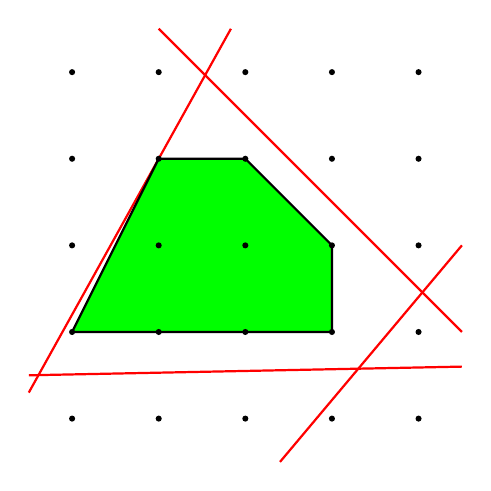
\begin{tikzpicture}[scale=1.1]

  \coordinate (a1) at (-0.5, 0.5);
  \coordinate (a2) at ( 4.5, 0.6);

  \coordinate (b1) at ( 2.4, -0.5);
  \coordinate (b2) at ( 4.5,  2.0);

  \coordinate (c1) at ( 4.5,  1.0);
  \coordinate (c2) at ( 1.0,  4.5);

  \coordinate (d1) at (-0.5,  0.3);
  \coordinate (d2) at ( 1.8333,  4.5);

  \draw[-,red,thick] (a1) -- (a2);
  \draw[-,red,thick] (b1) -- (b2);
  \draw[-,red,thick] (c1) -- (c2);
  \draw[-,red,thick] (d1) -- (d2);

  \coordinate (i1) at ( 0.0, 1.0);
  \coordinate (i2) at ( 3.0, 1.0);
  \coordinate (i3) at ( 3.0, 2.0);
  \coordinate (i4) at ( 2.0, 3.0);
  \coordinate (i5) at ( 1.0, 3.0);

  \draw[thick,fill=green] (i1) -- (i2) -- (i3) -- (i4) -- (i5) --cycle;

    \foreach \i in {0,...,4} {
       \foreach \j in {0,...,4} {
          \fill (\i,\j) circle (1.0pt);
       }
    }


  \end{tikzpicture}
\end{center}
\caption{\label{fig::integer_hull}
A polyhedron $P$ (given by the red hyperplanes) and its integer hull $P_I$ (green).
The black dots indicate the integral vectors.}
\end{figure}


\linebox{
\definition{
A polyhedron $P \subseteq \R^n$ is called
{\hi rational}\index{Rational polyhedron} if there are
$A \in \Q^{m \times n}$ and
$b \in \Q^{m}$ with $P = \{x \in \R^n \mid Ax \leq b\}$.\\
}
}


{\bf Observations:}
\begin{itemize}
   \item For a rational polyhedral cone (i.e.\ a cone 
         $C = \{x \in \R^n \mid  Ax\leq 0\}$ with $A \in \Q^{m \times n}$), we have
         $C_I = C$ (because a polyhedral cone is rational if and only if it is
         generated by a finite number of integral vectors).
   \item If $A$ is not rational, then $P_I$ is not necessarily a polyhedron. For example, let $P=\{x\in\R^n\mid x_1\ge 0\, , -\sqrt{2}x_1+x_2\le 0\}$; we leave it as an exercise to verify that $P_I$ is not a polyhedron.
   \item If $P$ is a polytope, then $P_I$ is a  polyhedron.
\end{itemize}




\linebox{
\theorem[The Fundamental Theorem of Integer Programming, Meyer, 1974]{\label{theorem::P_I_polyhedron}
Let $P = \{x \in \R^n \mid Ax \leq b\}$ be a rational polyhedron with
$A \in \Q^{m \times n}$ and $b \in \Q^m$. Then, $P_I$ is a polyhedron.\\
}
}





\prove
Let $P = \{x \in \R^n \mid Ax \leq b\}$ with
$A \in \Q^{m \times n}$ and $b \in \Q^m$.
By Theorem~\ref{theorem::polyhedron_decomposition}, we can write
$P = \text{conv}(V) + \text{cone}(E)$ for two finite sets
$V,E \subseteq \R^n$. Moreover, the proof of
Theorem~\ref{theorem::polyhedron_decomposition} also shows
that we can assume
that the elements of $V$ and $E$ are rational vectors. Hence, we can
even assume that $E=\{y_1,\dots,y_s\}$ where $y_i$ are integral vectors
($i=1,\dots,s$). Define 
$B := \{\sum_{i=1}^s \lambda_i y_i 
      \mid 0 \leq \lambda_i \leq 1 \text{ for } i \in \{1,\dots,s\} \}$.

Claim: $P_I = (\text{conv}(V) + B)_I + \text{cone}(E)$.

Proof of the claim: ``$P_I \subseteq (\text{conv}(V) + B)_I + \text{cone}(E)$'':\\
Let $p$ be an integral vector of $P$. Then, $p = q + c$ for some
$q \in \text{conv}(V)$ and some $c \in \text{cone}(E)$.
We can write $c = \sum_{i=1}^s \mu_i y_i$ with $\mu_i \geq 0$ for
$i \in \{1,\dots,s\}$. Therefore
$c = \sum_{i=1}^s \mu_i y_i = 
\underbrace{\sum_{i=1}^s  (\mu_i - \lfloor \mu_i \rfloor) y_i }_
{\in B}
+ 
\underbrace{\sum_{i=1}^s  \lfloor \mu_i \rfloor y_i }_
{\in (\text{cone}(E) \cap \Z^n)}$, so we can write
$c = b + c'$ with $b \in B$ and $c' \in \text{cone}(E) \cap \Z^n$.
Thus, $p = (q + b) + c'$. We have $q + b \in \text{conv}(V) + B$.
And $q + b = p - c'$, so $q + b$ is integral. Hence, $q + b \in (\text{conv}(V) + B)_I$,
and therefore $p \in (\text{conv}(V) + B)_I + \text{cone}(E)$.

``$P_I \supseteq (\text{conv}(V) + B)_I + \text{cone}(E)$'':\\
We have
\[
   (\text{conv}(V) + B)_I + \text{cone}(E) 
       \subseteq P_I + \text{cone}(E)
       = P_I + (\text{cone}(E))_I
       \subseteq (P + \text{cone}(E))_I 
       = P_I.
\]
This proves the claim.

The claim implies the statement of the theorem because
$\text{conv}(V) + B$ is a polytope, so
$(\text{conv}(V) + B)_I$ is also a polytope. This shows that
$P_I$ can be written as the Minkowski sum of two polyhedra.
However, by an earlier exercise, the Minkowski sum of two polyhedra
is again a polyhedron.
\endproof


In particular, we get the (somewhat surprising) consequence that 
one can solve integer linear programs by solving linear programs.
The problem is that the polyhedron $P_I$ may not have a simple 
description even if there is one for $P$. For example, 
\cite{Rub70} has shown that for any $k$ there are rational polyhedra 
$P \subseteq \R^2$ with only $3$ facets such that $P_I$ has more than
$k$ facets. Moreover, \cite{BarHL92} gave an a example showing that
there are rational polyhedra 
$P = \{x \in \R^n \mid Ax \leq b\} \subseteq \R^n$ such that
$P_I$ has $\Omega(\phi^{n-1})$ vertices, where 
$\phi = \text{size}(A) + \text{size}(b)$.




\linebox{
\proposition{\label{proposition::bound_P_I}
Let $P = \{ x \in \R^n \mid Ax \leq b \}$ with $A \in \Q^{m \times n}$ and
$b \in \Q^{m}$ such that $P_I \neq \emptyset$. Let $c \in \R^n$ be a vector.
Then, $\max\{c^t x \mid x \in P\}$ is bounded if and only if
$\max\{c^t x \mid x \in P_I\}$ is bounded.\\
}
}

\prove
``$\Rightarrow$:'' trivial.

``$\Leftarrow$:'' Assume that $\max\{c^t x \mid x \in P\}$ is unbounded.
Then, the dual LP must be infeasible, so there is no vector $y$ with
$A^t y = c$ and $y \geq 0$. By Farkas' Lemma (Theorem~\ref{theorem::farkas2}),
this means that there is a vector $z$ with $c^t z < 0$ and $A z \geq 0$.
Thus, the LP $\min\{c^t x \mid Ax \geq 0, -\one \leq x \leq \one\}$ is feasible
and has an optimum solution with negative value. 
By Proposition~\ref{theorem::SmallSolutions}, there is a rational optimum
solution $x^*$. By multiplying $x^*$ by an appropriate integer, we get
an integral vector $w$ with $A w \geq 0$ and $c^tw < 0$. Hence, for any
$v \in P_I$ and $k \in \N$ we have $v - kw \in P_I$. Therefore,
$\max\{c^t x \mid x \in P_I\}$ is unbounded.
\endproof


%%%%%%%%%%%%%%%%%%%%%%%%%%%%%%%%%%%%%%%%%%%%%%%%%%%%%
\subsection{Integral Solutions of Equation Systems}\label{sec::hermite}
%%%%%%%%%%%%%%%%%%%%%%%%%%%%%%%%%%%%%%%%%%%%%%%%%%%%%

In this section, our goal is to find a certificate that a
given system of equations does {\it not} have any integral
solution (which will be the result of 
Corollary~\ref{corollary::integral_solution}).


\linebox{
\definition{
An $m \times n$-matrix $A$ is in
{\hi Hermite normal form}{\index{Hermite normal form}}
if it can be
written as $A = \big[B \mid 0\big]$ where $B$ is a nonsingular lower
triangular non-negative matrix such that each row of $B$ has a unique
maximum entry and this maximum entry is on the diagonal.\\
}
}

The following operations on matrices are called {\hi elementary unimodular
column operations}:{\index{Elementary unimodular column operation}}
\begin{itemize}
   \item Exchange two columns.
   \item Multiply a column by $-1$.
   \item Add an integral multiple of one column to another column.
\end{itemize}


\linebox{
\theorem{
Each matrix $A \in \Q^{m \times n}$ of rank $m$ can be transformed into
a matrix in Hermite normal form by a series of elementary unimodular
column operations.\\
}
}

\prove
We may assume that $A$ is integral.
If this is not the case, we first multiply the matrix with 
an appropriate integer $M$ such that all entries are integral.
Then, we perform the following steps, and in the end, we divide 
the resulting matrix by $M$.
 
Assume that we have already transformed $A$ into a matrix
$\left[
   \begin{array}{cc}
      F & 0 \\
      G & H 
   \end{array}
\right]$
where $F$ is a lower
triangular matrix with positive diagonal.
Let $h_{11},\dots,h_{1k}$ be the first row of $H$.
Apply elementary unimodular column operations to
$H$ such that all $h_{1j}$ are non-negative and such that
$\sum_{j=1}^kh_{1j}$ is as small as possible. 
Since all entries are integer, this can be done with a 
finite number of operations. We may assume further that 
$h_{11} \geq h_{12} \geq \dots \geq h_{1k}$.
Then, $h_{11} > 0$ because $A$ has rank $m$.
Moreover, $h_{1j} = 0$ for $j \in \{2,\dots,k\}$ because
otherwise subtracting $h_{1j}$ from $h_{11}$ would
reduce $\sum_{j=1}^kh_{1j}$. Hence, we have obtained a
larger lower triangular matrix $F'$.

We iterate this step and end up with a matrix
$\big[B \mid 0\big]$ where $B$ is a lower triangular matrix with
positive diagonal. Denote the entries of $B$ be $b_{ij}$ 
($i=1,\dots,m$, $j =1,\dots,m$).
Finally, we perform for $i = 2,\dots,m$
the following steps: For $j=1,\dots,i-1$ add an integer multiple
of the $i$-th column of $B$ to the $j$-th column of $B$ such that
the $b_{ij}$ is non-negative and less than $b_{ii}$.
%Theorem 4.1 of \cite{Sch86}
\endproof


\linebox{
\corollary{\label{corollary::integral_solution}
Let $A \in \Q^{m \times n}$ and $b \in \Q^{m}$.
Then, $Ax = b$ has an integral solution $x$ if and only if
$b^t y$ is integral for each $y \in \Q^m$ for which $A^t y$
is integral.\\ 
}
}

\prove
%Corollary 4.1a of \cite{Sch86}
``$\Rightarrow$:'' If $x$ and $y^t A$ are integral vectors
and $Ax = b$, then $y^t A x = y^t b$ is also integral.

``$\Leftarrow$:'' Assume that $b^t y$ is integral for each
$y \in \Q^m$ for which $A^t y$ is integral.
Then, $Ax = b$ must have a (fractional) solution, since otherwise, by
Farkas' Lemma (Corollary~\ref{theorem::farkas3}), there would be 
a vector $y \in \Q^m$ with $y^t A = 0$ and $y^t b = -\frac{1}{2}$.
Thus, we may assume that the rows of $A$ are linearly independent,
so $A$ has rank $m$.

It is easy to check the statement to be proved holds for $A$ if and
and only if it holds for any matrix $\tilde A$, where $\tilde A$ arises
from $A$ by applying an elementary unimodular column operation.
Hence, we can assume that $A$ is in Hermite normal form
$\left[ B \, 0 \right]$. Thus, $B^{-1} \left[B \, 0 \right] 
= \left[I_m \, 0 \right]$ is an integral matrix.
Therefore by our assumption (applied to the rows of $B^{-1}$),
$B^{-1}b$ is an integral vector.
Since 
$\left[ B\, 0 \right] \left( \begin{array}{c} B^{-1}b \\ 0 \end{array}   \right) = b$,
the vector $x:= \left( \begin{array}{c} B^{-1}b \\ 0 \end{array}   \right)$ is
an integral solution for $\left[ B\, 0 \right]x = b$.
\endproof

\linebox{
\corollary{\label{corollary::computation_of_integer_solutions}
There is a polynomial-time algorithm that,
given $A \in \Q^{m \times n}$ and $b \in \Q^{m}$,  
computes an integral solution of $Ax=b$, provided that there
is one.\\
}
}

\prove
Transform $A$ into Hermite normal form 
$\left[B \, 0 \right]$
by elementary unimodular column operations,
which can be done in polynomial time.
Then, as in the proof of 
Corollary~\ref{corollary::integral_solution} 
compute an integer solution of 
$\left[B \, 0 \right] x = b$ which can be translated
into an integer solution of $Ax=b$ provided that 
we stored the elementary unimodular column operations
that have been applied.
\endproof

%%%%%%%%%%%%%%%%%%%%%%%%%%%%%%%%%%%%%%%%%%%%%%%%%%%%%
\subsection{Integral Polyhedra}\label{sub:integral_polyhedra}
%%%%%%%%%%%%%%%%%%%%%%%%%%%%%%%%%%%%%%%%%%%%%%%%%%%%%
A fundamental goal is to understand integral polyhedra, defined as:

\linebox{
\definition{
A polyhedron $P$ is called {\hi integral} if $P = P_I$.
{\index{Integral polyhedron}}\\
}
}
We now give some equivalent characterizations of integral polyhedra.

\linebox{
\theorem{\label{theorem::integrality_equivalence}
Let $P = \{ x \in \R^n \mid Ax \leq b \}$ with $A \in \Q^{m \times n}$ and
$b \in \Q^{m}$. Then, the following statements are equivalent:
\begin{itemize}
   \item[(a)] $P$ is integral
   \item[(b)] Each face of $P$ contains at least one integral vector.
   \item[(c)] Each minimal face of $P$ contains at least one integral vector.
   \item[(d)] Each supporting hyperplane  of $P$ contains at least one integral vector.
   \item[(e)] Each rational supporting hyperplane  of $P$ contains at least one integral vector.
   \item[(f)] $\max\{c^t x \mid x \in P \}$ is attained by an integral vector for each $c$
              for which the maximum is finite.
   \item[(g)] $\max\{c^t x \mid x \in P \}$ is an integer for each integral vector  $c$
              for which the maximum is finite.
\end{itemize}
}
}

\prove
The following implications are obvious: ``(b) $\Leftrightarrow$ (c)'', 
``(b) $\Rightarrow$ (d)'', ``(d) $\Rightarrow$ (e)'', and ``(f) $\Rightarrow$ (g)''

``(a) $\Rightarrow$ (b):'' Assume that $P$ is integral.
Let $F = P \cap H$ be a face of $P$ where 
$H = \{x \in \R^n \mid c^t x = \delta\}$ is a supporting hyperplane
of $P$. Then, any $z \in F$ is a convex combination of integral vectors
$v_1,\dots,v_k$ of $P$. If $v_i \in P \setminus F$ (so $c^t v_i < \delta$) for
an $i \in \{1,\dots,k\}$, then (since $c^t x = \delta$) there must be a
$j \in \{1,\dots,k\}$ with
$c^t v_j > \delta$, which is a contradiction to $v_j \in P$. Thus, all $v_i$
must be in $F$, so in particular $F$ contains an integral vector.

``(c) $\Rightarrow$ (f):'' Follows from Corollary~\ref{Corollary::faces}.

``(f) $\Rightarrow$ (a):'' Assume that (f) holds but $P \neq P_I$. Then, there is an
   $x^* \in P \setminus P_I$. By Theorem~\ref{theorem::P_I_polyhedron}, $P_I$ is a
   polyhedron, so there is an inequality $a^t x \leq \beta$ that is valid for 
   $P_I$ but not for $x^*$, so $a^t x^* > \beta$. This is a contradiction to (f)
   because $\max\{ a^tx \mid x \in P \}$ is finite 
   (by Proposition~\ref{proposition::bound_P_I}) but is not attained by any integral
   vector.

So far, we have proved that (a),(b),(c), and (f) are equivalent.

``(e) $\Rightarrow$ (c):'' We may assume that $A$ and $b$ are integral.
Let $F = \{x \in \R^n \mid A' x = b'\}$ be a minimal face of $P$
(where $A'x \leq b'$ is a subsystem of $Ax \leq b$). If there is no
integral vector $x$ with $A' x = b'$, then, by 
Corollary~\ref{corollary::integral_solution}, there must be a rational
vector $y$ such that $c:= (A')^t y$ is integral while $\delta := y^t b'$
is not an integer. Moreover, we may assume that all entries of $y$ 
are positive (otherwise we add an appropriate integral vector to $y$).
Since $c$ is integral but $\delta$ is not integral, the rational hyperplane
$H := \{x \in \R^n \mid c^t x = \delta\}$ does not contain any integral vector.

We will show that $H \cap P = F$ which implies that 
$H$ is a supporting hyperplane. 
By construction, we have $F \subseteq H$, so we have to show that
$H \cap P \subseteq F$. Let $x \in H \cap P$. 
Then, $y^t A' x = c^t x = \delta = y^t b'$, so $y^t(A' x - b') = 0$.
Thus, since all components of $y$ are positive,  $A'x = b'$, so
$x \in F$.

Now, we know that (a),(b),(c),(d),(e), and (f) are equivalent.

``(g) $\Rightarrow$ (e):'' Let $H = \{x \in \R^n \mid c^t x = \delta\}$
be a rational supporting hyperplane of $P$, so 
$\max\{ c^t x \mid x \in P \} = \delta$. Assume that $H$ does not contain
any integral vector. Then, by Corollary~\ref{corollary::integral_solution},
there is a positive number $\gamma$ for which $\gamma c$ is integral but $\gamma \delta$
is not integral. Then $\max\{  (\gamma c)^t x \mid x \in P\} 
= \gamma \max\{c^t x \mid x \in P\} = \gamma \delta \not\in \Z$, so
the statement of (g) is false.

Since ``(f) $\Rightarrow$ (g)'' is trivial, this shows the equivalence
of all statements.
\endproof

\linebox{
\corollary{
There is a polynomial-time algorithm which computes, given 
a rational polyhedron $P\subseteq \R^n$ with $P = P_I$ and a
rational vector $c$, a vector $x \in P \cap \Z^n$ maximizing $c^tx$
over $P \cap \Z^n$, provided that there is an optimum solution.\\
}
}

\prove
We only have to compute an integral element of a minimal
face $F$ consisting of optimum solutions only (for finding $F$
we can apply the {\sc Ellipsoid Method}). This can be done
by computing an integral solution of an equation system, which
can be done in polynomial time due to
Corollary~\ref{corollary::computation_of_integer_solutions}.
\endproof



%Moreover, by the equivalence of (f) and (g), the existence of an integral solution can be deduced from the integrality of the solution value. This motivates the following definition:


%%%%%%%%%%%%%%%%%%%%%%%%%%%%%%%%%%%%%%%%
\subsection{Total Unimodularity}\label{sec::TU}
%%%%%%%%%%%%%%%%%%%%%%%%%%%%%%%%%%%%%%%%


In this section, we want to identify integral matrices $A$ such that
$Ax \leq b, x \geq 0$ is integral for  any integer vector $b$.
% It will turn out that these are exactly the totally unimodular matrices (see Corollary~\ref{corollary::TU_TDI}).


\linebox{
\definition{
An $m \times n$-matrix $A$ with rank $m$ is called {\hi unimodular}{\index{Unimodular matrix}}
if $A \in \Z^{m \times n}$ and for all regular $m\times m$-submatrices
$B$ of $A$, we have $\text{det}(B) \in \{-1,1\}$.\\
}
}

In particular, a regular square matrix is unimodular if and only if
it is integral and its determinant is $-1$ or $1$.
Moreover, by Cramer's rule, the inverse of any unimodular square matrix
is an integral matrix.



{\bf Exercise:} Check that any series of elementary unimodular column operations,
applied to a matrix $A$ (see Chapter~\ref{sec::hermite}), can be performed by multiplying
$A$ from the right by an appropriate regular unimodular square matrix.


\linebox{
\definition{
A matrix $A$ is called {\hi totally unimodular} (TU){\index{Totally unimodular matrix}}
if every subdeterminant
of $A$ (i.e.\ every determinant of quadratic submatrices of $A$) is 
$0$, $-1$ or $1$.\\
}
}

In particular, all entries of totally unimodular matrices must be
$0$, $-1$ or $1$.




{\bf Observation:} A matrix $A\in\R^{m\times n}$ is totally unimodular if and only if
$\big[ I_m \mid A \big]\in \R^{m\times(m+n)} $ is unimodular.



\linebox{
\lemma{\label{eq:TU-transform}If $A\in\R^{m\times n}$ is TU, then the following matrices are also  TU:
The incidence matrix of a directed graph is totally unimodular: any submatrix $A'$ of $A$; $A^\top$; $A'$ obtained by multiplying a row or column of $A$ by $-1$; adding a unit vector as a row or as a column to $A$.
}
}



\linebox{
\theorem{\label{thm:TU-integral}
Let $A$ be a totally unimodular matrix, and let $b$ be an integral
vector. Then, the polyhedron $P = \{x \in \R^n \mid Ax \leq b \}$ is
integral.\\
}
}

\prove
%\cite{Sch86}, Theorem 19.1.
Let $F$ be a minimal face of $P$. We will show that $F$ contains 
an integral vector. By the implication ``(c) $\Rightarrow$ (a)''
of Theorem~\ref{theorem::integrality_equivalence} this is sufficient
to prove that $P$ is integral. 

By Proposition~\ref{proposition::minimal_faces}, we can write the
minimal face as $F = \{x \in \R^n \mid A'x = b'\}$ where
$A' x \leq b'$ is a subsystem of $Ax \leq b$. We can assume that
$A'$ has full row rank. By permuting coordinates, we can write
$A' = \big[ U \mid  V \big]$ for some matrix $U$ with 
$\text{det}(U) \in \{-1,1\}$. Thus $x := {U^{-1}b' \choose 0}$
is an integral vector in $F$.
\endproof


\linebox{
\theorem{\label{theorem::unimodular_integral}
Let $A\in \Z^{m \times n}$ be a matrix with rank $m$.
Then $A$ is unimodular if and only if
for each integral vector $b$ the polyhedron $\{x \in \R^n \mid Ax = b, x\geq 0\}$
is integral.\\
}
}

\prove
%\cite{Sch86}, Theorem 19.2.
``$\Rightarrow$:'' Assume that $A$ is unimodular, and let $b$ be an integral
vector. Let $x'$ be a vertex of $\{x \in \R^n \mid Ax = b, x \geq 0\}$.
This means that there are $n$ linearly independent constraints in the
system $Ax \leq b, -Ax \leq -b, -I_n x \leq 0$ that are satisfied by $x'$
with equality. Thus, the columns of $A$ corresponding to non-zero entries
of $x'$ are linearly independent. This set of columns can be extended to
a regular $m \times m$-submatrix $B$ of $A$. Then, the restriction of $x'$
to coordinates corresponding to $B$ is $B^{-1} b$. This is integral (because
$\text{det}(B) \in \{-1,1\}$). The other entries of $x'$ are zero, so $x'$
is integral.



``$\Leftarrow$:'' Suppose that $\{ x \in \R^n \mid Ax = b, x \geq 0\}$ is integral
for every integral vector $b$. Let $B$ be a regular $m\times m$-submatrix of $A$.
We have to show that $\det(B) \in \{-1,1\}$. To this end, it is sufficient to show
that $B^{-1}u$ is integral for every integral vector $u$ (by Cramer's rule). 
So let $u$ be an integral vector. Then, there is an integral vector $y$ such that
$z := y + B^{-1} u \geq 0$. Then, $b:= Bz$ is integral. Let $z'$ be a vector
with $Az' = Bz = b$ that arises from $z$ by adding zero-entries.
Then, $z'$ is a feasible (i.e.\ non-negative) basic solution of $Ax = b$,
so it is a vertex of $\{x \in \R^n \mid Ax = b, x \geq 0 \}$. Therefore
$z'$ is integral, which also shows that $z$ is integral.
This implies that $B^{-1}u = z - y$ is integral.
\endproof




\linebox{
\theorem\label{theorem::hoffman_kruskal}
(Hoffman \& Kruskal, \cite{HofK56})
Let $A$ be an integral matrix. Then $A$ is totally unimodular if and only if
for each integral vector $b$ the polyhedron $\{x \in \R^n \mid Ax \leq b, x\geq 0\}$
is integral.\\
}
}

\prove
%\cite{Sch86}, Corollary 19.2a.
The matrix $A$ is totally unimodular if and only if
$\big[I_m \mid A \big]$ is unimodular. Let $b$ be an integral vector.
Then, the vertices of $\{x \in \R^n \mid Ax\leq b, x \geq 0\}$ are integral
if and only if the vertices of 
$\{z \in \R^{m+n} \mid \big[ I_m \mid A \big] z = b, z \geq 0\}$
are integral. Thus, the statement follows from 
Theorem~\ref{theorem::unimodular_integral}.
\endproof




\linebox{
\corollary{\label{corollary::TU_both_integral}
An integral matrix $A$ is totally unimodular if and only if
for all integral vectors $b$ and $c$ optimum values for both
sides of the duality equation
\[
   \max\{c^t x \mid Ax \leq b, x \geq 0 \} =  \min\{b^t y \mid A^t y \geq c, y \geq 0 \}
\]
are attained by integral vectors (if they are finite).\\
}
}

\prove
%Corallary 19.2b from \cite{Sch86}
Follows directly from Hoffmans and Kruskal's Theorem 
(Theorem~\ref{theorem::hoffman_kruskal}) using the fact that a matrix
is totally unimodular if and only if its transposed matrix is totally
unimodular.
\endproof

\ifdefined\OnlineVersion{}\else

\linebox{
\lemma{
Let $Ax \leq b, x \geq 0$ with $A \in \R^{m\times n}$ and
$b \in \R^m$ be an inequality system. Suppose that for each
$c \in \Z^n$ for which $\min\{b^t y \mid A^t y \geq c, y \geq 0\}$
has an optimum solution, it has an optimum solution $y^*$ such that
the rows of $A$ corresponding to non-zero components of $y^*$
form a totally unimodular matrix. Then, $Ax \leq b, x \geq 0$ is
totally dual integral.\\
}
}

\prove
%Lemma 5.24 aus \cite{KorV18}
Let $c \in \Z^n$, and let $y^*$ be an optimum solution of
$\min\{ b^t y \mid A^t y \geq c, y \geq 0\}$ such that the rows
of $A$ corresponding to non-zero components of $y^*$ form a
totally unimodular matrix $\tilde A$. Let $\tilde b$ be the subvector of
$b$ consisting of the components corresponding to the rows of
$\tilde A$.

Claim: $\min\{b^t y \mid A^t y \geq c, y \geq 0\} 
      = \min\{\tilde b^t y \mid \tilde A^t y \geq c, y \geq 0\}$

Proof of the Claim: ``$\leq$:'' Any feasible solution of the 
right-hand side can by extended to a feasible solution of the left-hand side
with the same cost.

``$\geq$:'' Follows from the fact that $y^*$ is an optimum solution
of the left-hand side whose non-zero component provide a solution
of the right-hand side with the same cost. This proves the claim.

The matrix $\tilde A$ is totally unimodular, so by the
previous corollary, the system $\tilde A x \leq \tilde b$ is TDI.
Hence, the minimum on the right-hand in the above equation 
is attained by an integral vector. We can extend such an 
integral optimum solution by adding zero components to an integral
optimum solution of the left-hand side. This shows that 
$Ax \leq b, x \geq 0$ is TDI.
\endproof

\fi %onlineversion



We now consider some important
examples.
The {\hi incidence matrix}{\index{Incidence matrix}}
of an undirected graph $G$ is the matrix $A_G = (a_{v,e})_{v \in V(G) \atop e \in E(G)}$
which is defined by:
\[
   a_{v,e} = \left\{
      \begin{array}{ll}
         1, & \text{ if } v \in e\\
         0, &  \text{ if } v \not\in e
      \end{array}
\right.
\]
The {\hi incidence matrix}
of a directed graph $G$ is the matrix $A_G = (a_{v,e})_{v \in V(G) \atop e \in E(G)}$
which is defined by:
\[
   a_{v,(x,y)} = \left\{
      \begin{array}{ll}
         -1, & \text{ if } v = x\\
         1,  & \text{ if } v = y\\
         0,  & \text{ if } v \not\in \{x,y\}
      \end{array}
\right.
\]

\linebox{
\theorem{
The incidence matrix of a directed graph is totally unimodular.\\
}
}

\prove 
We show by induction on the size $k$ of the $k\times k$ submatrix $B$ of the incidence matrix $A$. The base case $k=1$ is immediate. Assume $k>1$. If any column of $B$ has a single nonzero entry, then $\det(B)=\pm\det(B')$ for a $(k-1)\times (k-1)$ submatrix $B'$, and the claim follows. Otherwise, every column of $B$ has two nonzero entries; but then one of these is 1 and the other is $-1$. Consequently, the sum of the rows of $B$ is 0, which means $\det(B)=0$.
\endproof

{\bf Remark:} This result gives a reason for the existence of integral optimum
solution of flow problems. These results can be extended to more general
linear functions on the edges of directed graphs (see exercises).




\linebox{
\theorem{\label{thm:bip-TU}
The incidence matrix of an undirected graph $G$ is totally unimodular
if and only if $G$ is bipartite.\\
}
}

\prove{
Assume first $G$ is bipartite with bipartition $(P,Q)$. Let $A_G$ denote its incidence matrix, and let $A'$ be the matrix where we multiply all rows corresponding to nodes in $P$ by $-1$. Then, $A'$ is the incidence matrix of a directed graph (where all edges are directed from $P$ to $Q$), and therefore TU by the previous theorem. By Lemma~\ref{eq:TU-transform}, this implies that $A_G$ is also $TU$.

Assume now $G$ is non-bipartite. Thus, $G$ contains an odd cycle $C$. Then, one can check that the determinant of the submatrix formed by the nodes and edges of $C$ is $2$.}
\endproof

{\bf Applications:}
\begin{itemize} 
   \item The previous theorem can be used to show 
{\hi K{\H o}nig's Theorem}:{\index{Koenig's Theorem@K\"onig's Theorem}}
The maximum cardinality of a matching in a bipartite
graph equals the minimum cardinality of a vertex cover. To see this,
let $G$ be a bipartite graph and $A_G$ its incident matrix.
Then, a maximum matching is given by an integral solution of
$\max\{ \one_m x \mid A_G x \leq \one_n, x \geq 0\}$ and a minimum vertex
cover by an integral solution of 
$\min\{ \one_n y \mid A_G^t y \geq \one_m, y \geq 0\}$. By the previous
theorem, $A_G$ is TU, so by Corollary~\ref{corollary::TU_both_integral}
both optima are attained by integral vectors.
   \item Another implication of the theorem provides a characterization of
{\hi doubly stochastic matrices}:\index{Doubly stochastic matrix}
A square matrix 
$M = (x_{ij})_{i=1,\dots,n \atop j=1,\dots,n} \in \R_{\geq 0}^{n \times n}$ is called
doubly stochastic if for all $i \in \{1,\dots,n\}$, we have
$\sum_{j=1}^n x_{ij} = 1$ and for all $j \in \{1,\dots,n\}$, we have
$\sum_{i=1}^n x_{ij} = 1$. If in addition all entries are integral,
we call the matrix a {\hi permutation matrix}.\index{Permutation matrix}
We claim that
each doubly stochastic matrix can be written as a convex combination
of permutation matrices (which has also been proved in an earlier exercise).
To see this, note that the set of all doubly stochastic $n \times n$-matrices
is given by $P = \{x \in \R^{n^2} \mid A_G x \leq \one, x \geq 0\}$ where $A_G$ is 
the incidence vector of the complete bipartite graph $K_{n,n}$ (which contains
a vertex for each column of $M$ in one side of the bipartition and
a vertex for each row of $M$ in the other side of the bipartition). Since
$A_G$ is TU, by Theorem~\ref{theorem::hoffman_kruskal} all vertices of
$P$ are integral, so the represent permutation matrices.
\end{itemize}

%Theorem 5.26 from + Exercise 11 from \cite{KorV18} 





The following theorem provides as a certificate to show that a 
matrix is totally unimodular.

\linebox{
\theorem{(Ghouila-Houri, \cite{Gho62})
\label{theorem::ghouila_houri}  %Ghouila-Houri; see 19.3 of \cite{Sch86}
A matrix $A = (a_{ij})_{{i=1,\dots,m}\atop{j=1,\dots,n}} \in \Z^{m \times n}$
is totally unimodular if and only if
for each set $R \subseteq \{1,\dots,n\}$ there are sets $R_1$ and $R_2$
with $R = R_1 \dot\cup R_2$ such that for each $i \in \{1,\dots,m\}$:
\[
   \sum_{j \in R_1}a_{ij} - \sum_{j \in R_2}a_{ij} \in \{-1,0,1\}.
\]
}
}

\prove
``$\Rightarrow$:'' Let $A$ be totally unimodular and $R \subseteq \{1,\dots,n\}$.
Let $d \in \{0,1\}^n$ be the characteristic vector for $R$, i.e.\
\[
   d_r = \left\{\begin{array}{ll}
           1 & \text{ for } r \in R\\
           0 & \text{ for } r \in \{1,\dots,n\}\setminus R
         \end{array}
         \right.
\]
Since $A$ is totally unimodular, also the matrix
$\left(\begin{array}{r}
A  \\
-A \\
I_n
\end{array}
\right)$ is also totally unimodular.
Thus, the polytope
\[
   P := \left\{
      x \in \R^n \mid   Ax \leq \left\lceil  \frac{1}{2} Ad \right\rceil, 
                        Ax \geq \left\lfloor \frac{1}{2} Ad \right\rfloor,
                        x \leq d, x \geq 0
   \right\}
\]
is integral. It contains the vector $\frac{1}{2}d$, so it is non-empty.
Let $z$ be an integral vertex of $P$. 
Then, for any $i \in \{1,\dots,m\}$, we have
$\sum_{j=1}^n a_{ij} z_j  \leq  \left\lceil \frac{1}{2} \sum_{j=1}^n a_{ij} d_j \right\rceil
\leq  \frac{1}{2} + \frac{1}{2} \sum_{j=1}^n a_{ij} d_j$ and
$\sum_{j=1}^n a_{ij} z_j  \geq  \left\lfloor \frac{1}{2} \sum_{j=1}^n a_{ij} d_j \right\rfloor
\geq  -\frac{1}{2} + \frac{1}{2} \sum_{j=1}^n a_{ij} d_j$, so
$-1 \leq \sum_{j=1}^n a_{ij} (d_j - 2z_j) \leq  1$.

Define $R_1 := \{r \in R \mid z_r = 0\}$ and $R_2 := \{r \in R \mid z_r = 1\}$.
For $i \in \{1,\dots,m\}$, this yields
\[
   \sum_{j \in R_1} a_{ij} - \sum_{j \in R_2} a_{ij} \, = \, \sum_{j=1}^n  a_{ij} (d_j - 2z_j) \, \in \, \{-1,0,1\}
\]

\RED{[[Second part of proof is non-examinable]]} 

``$\Leftarrow$:'' Assume that for each  $R \subseteq \{1,\dots,n\}$ there are
sets $R_1, R_2 \subseteq R$
with $R = R_1 \dot\cup R_2$ as described in the theorem.
We show by induction in $k$ that every $k \times k$-submatrix of $A$ has determinant $-1$, $0$ or $1$.
For $k = 1$ this follows from the criterion for $|R| = 1$.

Let $k > 1$. Let $B = (b_{ij})_{i,j \in \{1,\dots,k\}}$ be a submatrix of $A$.
We can assume that $B$ is non-singular because otherwise its determinant is $0$.

By Cramer's rule, each entry of $B^{-1}$ is $\frac{\text{det}(B')}{\text{det}(B)}$
where $B'$ arises from $B$ by replacing a column by a unit vector. By the 
induction hypothesis $\text{det}(B') \in \{-1,0,1\}$. 
Hence, all entries of the matrix $B^* := (\text{det}(B))B^{-1}$ are in $\{-1,0,1\}$.

Let $b^*$ be the first column of $B^*$. Then, $B b^* = \text{det}(B) e_1$ where
$e_1$ is the first unit vector. 
We define $R:= \{ j \in \{1, \dots, k\} \mid b^*_j \neq 0 \}$.
For $i \in \{2,\dots,k\}$, we have $0 = (B b^*)_i = \sum_{j \in R} b_{ij} b^*_j$,
so $|\{ j \in R \mid b_{ij} \neq 0 \}|$ is even.

Let $R = R_1 \dot\cup R_2$ such that 
$\sum_{j \in R_1} b_{ij} - \sum_{j \in R_2} b_{ij} \in \{-1,0,1\}$ for all $i \in \{1,\dots,k\}$.
Thus, for $i \in \{2,\dots,k\}$, we have (since $|\{ j \in R \mid b_{ij} \neq 0 \}|$ is even):
$\sum_{j \in R_1} b_{ij} - \sum_{j \in R_2} b_{ij} = 0$. If we also had
$\sum_{j \in R_1} b_{1j} - \sum_{j \in R_2} b_{1j} = 0$, then the columns of $B$ would
not be linearly independent. 
Hence, $\sum_{j \in R_1} b_{1j} - \sum_{j \in R_2} b_{1j} \in \{-1,1\}$ and
thus, $B x \in \{e_1,-e_1\}$ where the vector $x \in \{-1,0,1\}^k$ is defined
by
\[
   x_j = \left\{\begin{array}{ll}
           1  & \text{ for } j \in R_1\\
           -1 & \text{ for } j \in R_2\\
           0  & \text{ for } j \in \{1,\dots,k\}\setminus R
         \end{array}
         \right.
\]
Therefore, $b^* = \text{det}(B) B^{-1}e_1 \in \{\text{det}(B)x, -\text{det}(B)x\}$.
But both $b^*$ and $x$ are non-zero vectors with entries -1,0,1 only,
so we can conclude that $\text{det}(B) \in \{-1,1\}$.
\endproof

We use this theorem to give a new proof of Theorem~\ref{thm:bip-TU}:
\paragraph{Proof of Theorem~\ref{thm:bip-TU}:}
Let $G$ be an undirected graph and $A_G$ its incidence matrix.
Since a matrix is TU if and only if its transposed matrix
is TU, we can apply Theorem~\ref{theorem::ghouila_houri} to the rows of $A_G$:
$A_G$ is TU if and only if for each $X \subseteq V(G)$ there is a partition 
$X = A \dot\cup B$ with $E(G[A]) = E(G[B]) = \emptyset$. The last condition
is satisfied if and only if $G$ is bipartite.
\endproof



%%%%%%%%%%%%%%%%%%%%%%%%%%%%%%%%%%%%%%%%%%
\subsection{TDI Systems}
%%%%%%%%%%%%%%%%%%%%%%%%%%%%%%%%%%%%%%%%%%

\linebox{
\definition{
A system of inequalities $Ax \leq b$ is called {\hi totally dual integral}
({\hi TDI system}), {\index{Totally dual integral}}{\index{TDI system}}
if the LP $\min \{b^t y \mid A^t y = c, y \geq 0 \}$ has an integral
optimum solution for each integral vector $c$ for which the LP is feasible
and bounded.\\
}
}

Note that total dual integrality is in fact a property of the system of
inequalities, not just of the polyhedron that is defined by them.
For example the systems 
\[
\left(
   \begin{array}{rr}
     1 &  1 \\
     1 &  0 \\
     1 & -1 
   \end{array}
\right)
\left(
  \begin{array}{c}
     x_1 \\
     x_2 
  \end{array}
\right)
\leq 
\left(
  \begin{array}{c}
     0 \\
     0 \\
     0 
  \end{array}
\right)
\]
and
\[
\left(
   \begin{array}{rr}
     1 &  1 \\
     1 & -1 
   \end{array}
\right)
\left(
  \begin{array}{c}
     x_1 \\
     x_2 
  \end{array}
\right)
\leq 
\left(
  \begin{array}{c}
     0 \\
     0 
  \end{array}
\right)
\]
define the same polyhedron. But it is easy to check that the
first system of inequalities is TDI while the second one is not TDI.


\linebox{
\theorem{\label{theorem::TDI_integral}
Let $A \in \Q^{m\times n}$ and $b \in \Z^m$ such that $Ax \leq b$ is totally
dual integral. Then, the polyhedron $P = \{ x \in \R^n \mid Ax \leq b \}$ is
integral.\\
}
}

\prove
If $Ax \leq b$ is TDI, then by definition $\min \{b^t y \mid A^t y = c, y \geq 0 \}$
is an integer for each integral vector  $c$ for which the minimum is finite.
By duality, this implies that $\max \{c^t x \mid A x \leq b \}$
is an integer for each integral vector $c$ for which the maximum is finite.
Thus, by the implication ``(g) $\Rightarrow$ (a)'' of
Theorem~\ref{theorem::integrality_equivalence}, $P$ is integral.
\endproof


\linebox{
\proposition{\label{proposition::additional_constraints_still_TDI}
If $Ax \leq b$ is a TDI-system, and $a^t x \leq \beta$ is valid for
any $x \in \R^n$ with $Ax \leq b$, then the system 
$Ax \leq b, a^t x \leq \beta$ is also totally dual integral.\\
}
}

\prove
%\ifdefined\OnlineVersion{}
%Exercise.
%\else
Let  $Ax \leq b$ be a TDI-system, and $a^t x \leq \beta$ a valid inequality for
any $x \in \R^n$ with $Ax \leq b$. Let $c$ be an integral vector for which the LP
$\min \{b^t y +\beta \gamma \mid A^t y + \gamma a = c, y \geq 0, \gamma \geq 0 \}$ is
feasible and and bounded.
Then
\begin{eqnarray*}
   \min \{b^t y + \beta \gamma \mid A^t y + \gamma a = c, y \geq 0, \gamma \geq 0 \}
           & = & \max\{c^t x \mid Ax \leq b, a^t x \leq \beta\} \\
           & = & \max\{c^t x \mid Ax \leq b\} \\
           & = & \min \{b^t y \mid A^t y = c, y \geq 0 \}
\end{eqnarray*}
The last minimization problem has an optimum solution $y^*$ that is
integral. Together with $\gamma^* = 0$, this gives an optimum integral
solution for the first minimization problem.
%\fi %onlineversion
\endproof




Hence, if a system $Ax \leq b$ is not TDI, then no proper subsystem 
$A' x \leq \b'$ with $\{x \in \R^n \mid Ax \leq b\} = \{x \in \R^n \mid A'x \leq b'\}$
can be TDI. We call a system $Ax \leq b$ {\hi minimally TDI}{\index{Minimally TDI}}
if it
is TDI but no proper subsystem of $Ax \leq b$ defining the same
polyhedron is TDI.

\iffalse

\linebox{
\proposition{\label{proposition::faces_of_TDI_are_TDI}
If $Ax \leq b, a^t x \leq \beta$ is a TDI-system
with integral vector $a$, then
$Ax \leq b, a^t x = \beta$ is also a TDI-system.\\
}
}

\prove
%\cite{Sch86}, Theorem 22.2.
Let $c$ be an integral vector for which 
\begin{equation}\label{eq::TDI_max_min1}
\begin{array}{rcl}
   &   & \max\{ c^t x \mid Ax \leq b, a^t x = \beta  \} \\
   & = & \min\{b^t y + \beta(\lambda - \mu) \mid y \geq 0, \lambda,\mu \geq 0,
               A^t y + (\lambda - \mu)a = c\}
\end{array}
\end{equation}
is finite. Let $x^*,y^*,\lambda^*, \mu^*$ be optimum primal and dual
solutions. Set $\tilde c := c + \lceil \mu^* \rceil a$. Then,
\begin{equation}\label{eq::TDI_max_min2}
\begin{array}{rcl}
   &   & \max\{ \tilde c^t x \mid Ax \leq b, a^t x \leq \beta  \}\\
   & = & \min\{b^t y + \beta \lambda \mid y \geq 0, \lambda \geq 0,
               A^t y + \lambda a = \tilde c\}
\end{array}
\end{equation}
is finite because $x^*$ is feasible for the maximum and $y^*$ and
$\lambda^* + \lceil \mu^* \rceil - \mu^*$ are feasible for the minimum.

Since $Ax \leq b, a^t x \leq \beta$ is a TDI-system, the minimum in 
equation (\ref{eq::TDI_max_min2})
has an integer optimum solution $\tilde y, \tilde \lambda$.
Then, $y := \tilde y$, $\lambda := \tilde \lambda$, $\mu := \lceil \mu^* \rceil$
is an integer optimum solution for the minimum in (\ref{eq::TDI_max_min1}):
it is obviously feasible, and its cost is:
\[
   b^t \tilde y + \beta(\tilde \lambda - \lceil \mu^* \rceil )
     \, = \,    b^t \tilde y + \beta \tilde \lambda - \beta \lceil \mu^* \rceil
     \, \leq \, b^t y^* + \beta (\lambda^* + \lceil \mu^* \rceil - \mu^*) 
          - \beta \lceil \mu^* \rceil
     \, = \,    b^t y^* + \beta (\lambda^*  - \mu^*).
\]
The inequality follows from the fact that
$y^*$, $\lambda^* + \lceil \mu^* \rceil - \mu^*$ is feasible for the minimum
in (\ref{eq::TDI_max_min2}) and $\tilde y$, $\tilde \lambda$ is an optimum
solution for the minimum in (\ref{eq::TDI_max_min2}).
Hence, the minimum in (\ref{eq::TDI_max_min1}) has an integral optimum solution,
so $Ax \leq b, a^t x = \beta$ is TDI.
\endproof



\linebox{
\definition{
%-Definition Hilbert basis
A finite set of vectors $\{v_1,\dots,v_t\}$ is a {\hi Hilbert basis}{\index{Hilbert basis}}
if each integral vector in $\text{cone}(\{v_1, \dots, v_t\})$ is a non-negative
integral combination of  $v_1,\dots,v_t$.\\
}
}

{\bf Example:} The set of the standard unit vectors together with their negatives is
a Hilbert basis of the cone $\R^n$.


\linebox{
\theorem{
Every rational polyhedral cone is generated by an integral Hilbert basis.\\
}
}

\prove
%-Lemma: Existence of a Hilbert basis (Theorem 16.4 \cite{Sch86}, ohne Eindeutigkeit)
Let $C$ be a rational polyhedral cone. $C$ is generated by some rational vectors
$b_1,\dots,b_k$, and we can assume with loss of generality that these vectors are
integral. Let $H$ consist of all integral vectors in 
\[
  P = \left\{\sum_{i=1}^k \lambda_i b_i \mid 0 \leq \lambda_i \leq 1 \text{ for }i \in \{1,\dots,k\} \right\}.
\]
Obviously $H$ is a finite set.
We claim that $H$ is a Hilbert basis generating $C$. As 
$\{b_1,\dots,b_k\} \subseteq H \subseteq C$, the cone $C$ is generated by $H$. 
To see that $H$ forms a Hilbert basis, let $b$ be an integral vector in $C$. 
Since $b_1,\dots,b_k$ generate $C$, there are nonnegative numbers $\mu_1,\dots,\mu_k$ with
$b = \sum_{i=1}^k \mu_i b_i$, so
\[
   b = \left( \sum_{i=1}^k \lfloor \mu_i \rfloor b_i \right) + 
       \sum_{i=1}^k ( \mu_i - \lfloor \mu_i \rfloor) b_i.
\]
Then, the vector
\[
   b - \left( \sum_{i=1}^k \lfloor \mu_i \rfloor b_i \right) = \sum_{i=1}^k ( \mu_i - \lfloor \mu_i \rfloor) b_i
\]
is integral and an element of $P$.
Thus (since $\{b_1,\dots,b_k\} \subseteq H$), $b$ can be 
written a a non-negative integral combination of the elements of $H$. This shows
that $H$ is a Hilbert basis.
\endproof

{\bf Notation:} For a system of inequalities $Ax \leq b$ and 
a face $F$ of $\{x \in \R^n \mid Ax \leq b\}$, we call a row of $A$
{\hi active}, if the corresponding inequality in $Ax \leq b$ is satisfied 
with equality for all $x \in F$.{\index{Active row}}

\linebox{
\theorem{\label{theorem::TDI_Hilbert}
A feasible rational system of inequalities $Ax \leq b$ is TDI if and only if for each
minimal face $F$ of $P := \{x \in \R^n \mid Ax \leq b\}$, the rows that are active in $F$
form a Hilbert basis.\\
}
}

\prove
%Theorem 22.5 of \cite{Sch86}.
``$\Rightarrow$:'' Suppose that $Ax \leq b$ is TDI. Let $F$ be a minimal
face of $P$ and let $a_1,\dots,a_t$ be the rows of $A$ that are active for $F$.
We have to show that $\{a_1,\dots,a_t\}$ is a Hilbert basis. Let $c$ be an integral
vector in $\text{cone}(\{a_1,\dots,a_t\})$. We have to 
write $c$ as an integral non-negative combination of $a_1,\dots,a_t$.
The maximum in the LP-duality equation
\begin{equation} \label{eq::hilbert_primal_dual}
   \max\{c^t x \mid Ax \leq b \} = \min \{b^ty \mid A^t y = c, y \geq 0\}
\end{equation}
is attained by every vector $x$ in $F$. Since $Ax \leq b$ is TDI, the dual
problem has an integral optimum solution $y$. By complementary slackness, the
entries of $y$ at positions corresponding to rows that are not active in $F$
are $0$. Thus, $c$ is an integral non-negative combination of $a_1,\dots,a_t$.

``$\Leftarrow$:'' Assume that for each minimal face $F$ of $P$,
the rows that are active in $F$ form a Hilbert basis.
Let $c$ be an integral vector for which the optima in
(\ref{eq::hilbert_primal_dual}) are finite. 
We have to show that the minimum is attained by an integral vector.
Let $F$ be a minimal face of $P$ such that each vector in $F$ attains the maximum 
in the duality equation. Let $a_1,\dots,a_t$ be rows of $A$ that are active in $F$.
Then, by complementary slackness, $c \in \text{cone}(\{a_1,\dots,a_t\})$.
Since $a_1,\dots,a_t$ form a Hilbert basis, we can write 
$c= \sum_{i=1}^t \lambda_i a_i$ for certain non-negative integral numbers 
$\lambda_1,\dots,\lambda_t$. We can extend $(\lambda_1,\dots,\lambda_t)$ 
with zero-components to a vector $y \in \Z^m$ with $y \geq 0$, $A^t y = c$
and $b^t y = x^t A^t y = c^t x$ for all $x \in F$. In other words,
$y$ is an integral optimum solution of the dual LP.
\endproof


\ifdefined\OnlineVersion{}\else

{\bf Observation:} A TDI-system is minimally TDI if and only if each constraint in
$Ax \leq b$ defines a supporting hyperplane of $\{x \in \R^n \mid Ax \leq b\}$ and 
is not a non-negative integral combination of other constraints in $Ax \leq b$.

Schrijver [1979] (On total dual integrality) has shown that for any rational 
polyhedron $P$ of full dimension there is a unique minimal TDI system 
$Ax \leq b$ with A integral and $b$ rational such that 
$P = \{x \in \R^n \mid Ax \leq b\}$
 

\fi %onlineversion


\linebox{
\theorem{
The rational system of inequalities $A x \leq 0$ is TDI if and only if
the rows of $A$ form a Hilbert basis.\\
}
}

\prove
Follows from the previous Theorem with $b = 0$ (note that in the unique minimal face of
$\{x \in \R^n \mid Ax \leq 0\}$ all rows of $A$ are active).
\endproof

\fi
%Chapter 22.3 \cite{Sch86}

The following theorem by  Giles and Pulleyblank from 1979 states that every polyhedron can be described by a TDI system; we do not prove it here.

\linebox{
\theorem{(\cite{GilP79})\label{theorem::giles_pulleyblank}
For each rational polyhedron $P \subseteq \R^n$ there exists a rational TDI-system
$Ax \leq b$ with $A \in \Z^{m \times n}$ and $P = \{x \in \R^n \mid Ax \leq b \}$.
The vector $b$ can be chosen to be integral if and only if $P$ is integral.\\
}
}

\iffalse
\prove
We can assume w.l.o.g.\ that $P \neq \emptyset$.
For each minimal face $F$ of $P$, we define
\[
   C_F := \{c \in \R^n \mid c^tz = \max\{c^tx \mid x \in P\} \text{ for all } z \in F\}.
\]
Then, $C_F$ is a polyhedral cone. %siehe 5.18 KorV18 
To see this, assume that $P=\{\tilde A x \leq \tilde b\}$ is some 
description of $P$. Then 
$C_F$ is generated by the rows of $\tilde A$ that are active in $F$.

Let $F$ be a minimal face, and let $a_1,\dots,a_t$ be an integral Hilbert basis generating
$C_F$. Choose $x_0 \in F$, and define $\beta_i := a_i^t x_0$ for $i=1,\dots,t$.
Then, $\beta_i = \max\{a_i^t x \mid x \in P\}$ ($i=1,\dots,t$). Let $\mathcal{S}_F$
be the system $a_1^t x \leq \beta_1, \dots, a_t^tx \leq \beta_t$. All inequalities in
$\mathcal{S}_F$ are valid for $P$. Let $Ax \leq b$ be the union of the systems
$\mathcal{S}_F$ over all minimal faces $F$ of $P$. 
Then, $P \subseteq \{x \in \R^n \mid Ax \leq b\}$. On the other hand, if 
$x^* \in \R^n \setminus P$, then there is a supporting hyperplane of $P$
separating
$x^*$ from $P$, and this supporting hyperplane touches $P$ in a minimal face, so
there is an inequality in $Ax \leq b$ that is violated by $x^*$. Hence,
$P = \{x \in \R^n \mid Ax \leq b\}$. Moreover, by Theorem~\ref{theorem::TDI_Hilbert},
$Ax \leq b$ is TDI.

If $P$ is integral, then all the $\beta_i$ can chosen to be integral because we 
can choose the vectors $x_0 \in F$ as integral vectors.
On the other hand, if
$b$ is integral, then by Theorem~\ref{theorem::TDI_integral}, $P$ is integral.
\endproof

\fi
\ifdefined\OnlineVersion{}\else


In the primal-dual $\max\{c^t x \mid Ax \leq b \} = \min \{b^ty \mid A^t y = c, y \geq 0\}$
we know (by the {\sc Simplex Algorithm})
that if both optima are finite, the minimization problem has an optimum
solution $y$ with at most $\text{rank}(A)$ non-zero entries.
If we ask for an optimum
{\it integral} solution (with $Ax \leq b$ TDI and $b$ integral), this is not necessarily the case:
see $A = {2 \choose -3}$, $b = {0 \choose 0}$ and $c = (1)$. Nevertheless, for full-dimensional
solution spaces, we get
the following bound on the number of non-zero entries:

\linebox{
\theorem{
Let $Ax \leq b$ be a TDI-system with $A \in \Z^{m \times n}$ such that
$\text{dim}(\{x \in \R^n \mid Ax \leq b\}) = n$. Let $c$ be an integral
vector for which the optima in 
\[
   \max\{c^t x \mid Ax \leq b \} = \min \{b^ty \mid A^t y = c, y \geq 0\}
\]
are finite. Then, the minimization problem has an integral optimum solution
$y$ with at most $2r - 1$ positive components where $r := \text{rank}(A)$.\\
}
}

\prove %22.12 Schrijver
{\bf Claim:} Let $\{a_1,\dots,a_t\} \subseteq \Z^n$ be a Hilbert basis such that 
$C := \text{cone}(\{a_1,\dots,a_t\})$ is a pointed $k$-dimensional polyhedral cone.
Then, any integral vector
$c$ in $C$ is a nonnegative integral combination
of at most $2k-1$ vectors in $a_1,\dots,a_t$

{\bf Proof of the Claim:}
Let $\lambda_1,\dots,\lambda_t$ attain 
\begin{equation}\label{eq::small_Hilbert_basis}
   \max\left\{\sum_{i=1}^{t} \lambda_i \mid \lambda_1,\dots,\lambda_t \geq 0; c= \sum_{i=1}^t\lambda_i a_i\right\}
\end{equation}
Since $C$ is pointed, the maximum is finite (check that the dual LP
$\min\{c^t y \mid y^t a_i \geq 1 \text{ for } i \in \{1,\dots,t\}\}$
is feasible).
We can assume that at most $k$ of the $\lambda_i$ are non-zero. Define
\[
   c' := c - \sum_{i=1}^t \lfloor \lambda_i \rfloor a_i 
       = \sum_{i=1}^t (\lambda_i - \lfloor \lambda_i \rfloor) a_i.
\]
Then, $c'$ is an integral vector in $C$, so we can write it as
$ c' = \sum_{i=1}^t \mu_i a_i$
for some integral numbers $\mu_1,\dots,\mu_t \geq 0$.
Since $\lambda_1,\dots,\lambda_t$ was an optimum solution of 
(\ref{eq::small_Hilbert_basis}) and 
$\mu_1 + \lfloor \lambda_1 \rfloor, \dots, \mu_t + \lfloor \lambda_t \rfloor$ is
a feasible solution, we have 
$\sum_{i=1}^t \mu_i + \sum_{i=1}^t \lfloor \lambda_i \rfloor \leq \sum_{i=1}^t \lambda_i$,
so
\[
   \sum_{i=1}^t \mu_i \leq  \sum_{i=1}^t \lambda_i - \sum_{i=1}^t \lfloor \lambda_i \rfloor < k
\]
because at most $k$ of the $\lambda_i$ are non-zero. Thus, at most $k-1$ of the
$\mu_i$ are non-zero. Therefore, the decomposition
\[
   c = \sum_{i=1}^t (\lfloor \lambda_i \rfloor + \mu_i) a_i
\]
has at most $2k - 1$ non-zero components.
This proves the claim.

The claim implies the statement of the theorem. To see this, first note that
if $P := \{x \in \R^n \mid Ax \leq b\}$ is full-dimensional, then a cone generated
by rows of $A$ that are active in a minimal face $F$ of $P$ 
must be pointed. Otherwise such a cone would contain a pair of vectors $v$ and $-v$.
Thus there would be inequalities
$v^t x \leq \beta_1$ and $-v^t x \leq \beta_2$ (for some numbers
$\beta_1,\beta_2$) that can be written as non-negative combinations of 
inequalities in $Ax \leq b$ corresponding to rows of $A$ that are active in $F$.
For $x \in F$ we have 
$v^t x = \beta_1$ and $-v^t x = \beta_2$, 
so this would imply $\beta_1 = -\beta_2$
and $P$ would be contained in $\{x \in \R^n \mid v^t x = \beta_1\}$,
which is a contradiction to the assumption that $P$ is full-dimensional.

By Theorem~\ref{theorem::TDI_Hilbert},
the rows that are active for a minimal face consisting of optimum 
solutions of $\max\{c^t x \mid Ax \leq b \}$ form a Hilbert basis (because
$Ax \leq b$ is TDI). 
%Finally, we can assume that the vectors $a_1,\dots,a_t$ are in $\Z^k$ where
%$k$ is the dimension of the subspace spanned by $a_1,\dots,a_t$.
%Theorem 22.12 \cite{Sch86}
\endproof

\fi %onlineversion

%Def. 5.28 and Theorem 5.29 aus \cite{KorV18}

%Dann Nash-Williams 22.4 aus \cite{Sch86}

Theorem~\ref{theorem::hoffman_kruskal} shows a connection between totally unimodular matrices and TDIness.

\linebox{
\corollary{\label{corollary::TU_TDI}
An integral matrix $A$ is totally unimodular if and only if 
the system $Ax \leq b, x \geq 0$ is TDI for each vector $b$.\\
}
}

\prove
%Corollary 5.23 aus \cite{KorV18}
``$\Rightarrow$:'' If $A$ is totally unimodular, then also $A^t$
is totally unimodular. 
Thus, by Theorem~\ref{theorem::hoffman_kruskal}, 
$\min\{b^t y \mid A^t y \geq c, y \geq 0\}$ is attained by an 
integral vector for each vector $b$ and each integral vector $c$
for which the minimum is finite. This implies that the system
$Ax \leq b, x \geq 0$ is TDI for each vector $b$.

``$\Leftarrow$:'' Suppose that $Ax \leq b, x \geq 0$ is TDI
for each vector $b$. By Theorem~\ref{theorem::TDI_integral} this implies
that the polyhedron $\{x \in \R^n \mid Ax \leq b, x \geq 0\}$ is
integral for each integral vector $b$. 
By Theorem~\ref{theorem::hoffman_kruskal}, this means that $A$ is 
totally unimodular.
\endproof

\subsection{Cutting Planes}

The general strategy of cutting-plane methods can be described as follows:
\iffalse
Assume that we are given a polyhedron $P$ and we want to optimize
a linear function over the integral vectors in $P$. To this end, we first find an
optimum solution $x^*$
over $P$. If this belongs to $P_I$, we are done, because then we
can also easily compute and integral solution of the same cost. Otherwise
we look for an hyperplane separating $x^*$ from $P_I$, so we ask for a vector
$c$ and a number $\delta$, such that $a^t x \leq \beta$ for all $x \in P_I$
but $a^t x^* > \beta$. Then, we add the constraint  $c^t x \leq \delta$,
solve the linear program again and iterate these steps until we get an integral
solution.


More formally,\fi
Suppose we want to solve a given integer optimization problem
\begin{equation}\label{eq:IP-cut}\begin{array}{rl}
\max &c^t  x \\
Ax&\le b\\
x&\in\mathbb{Z}^n\, 
\end{array}\hfill \end{equation}
for a given matrix $A\in\Q^{m\times n}$ and vector $b\in\Q^m$.

We let $P=\{x\in\R^n\mid Ax\le b\}$; thus, othe goal is to find an integer point $x\in P\cap \Z^n$ maximizing $c^t x$. This is equivalent to solving 
\[ \max c^t x\quad\mbox{s.t.}\quad x\in P_I\]

We say that a linear inequality  $a^t  x\leq \beta$, (where $a\in\R^n$, $\beta\in \R$) is {\em valid} for $P_I$ if, for all $x\in P_I$, $a^t  x\leq \beta$ holds.
Given any point for $x^*\notin P_I$, we say that $a^t  x\leq \beta$ {\em cuts-off} $x^*$ if $a^t x^*>\beta$. 

At the high level, a cutting plane method can be summarized as follows.

\vspace{.4in}

\noindent\framebox[1.02\width][c]{\parbox{.96\textwidth}{
\center{\bf Cutting planes method}
\medskip

\noindent Define as initial LP relaxation the problem $\max\{c^\top x\mid Ax\leq b\}$.

\begin{enumerate}
\item Solve the current relaxation, and let $x^*$ be a basic  optimal solution;
\item If $x^*\in P_I$, then $x^*$ is an optimal solution to the MIP~\eqref{eq:IP-cut}, STOP.
\item Otherwise, \underline{find} a valid inequality $a^t x\leq \beta$ for $P_I$ cutting-off $x^*$;
\item Add the constraint $a^t  x\leq \beta$ to the current linear relaxation and return to 1.
\end{enumerate}}}
\vspace{.4in}

Obviously, the cutting plane method described here is a general technique to tackle (mixed) integer optimization problems, but to implement it is necessary to device an automatic way to generate valid inequalities cutting-off the current fractional solution. Such a valid inequality is usually referred to as a {\em cutting plane}.



\subsubsection{Gomory-Chv\'atal cuts}



How can we find half-space that contain $P_I$ but not necessarily
$P$? An easy observation is that if $H$ is a half-space that contains
$P$, then $P_I$ is contained in $H_I$. This motivates the following definition:

\linebox{
\definition{
Let $P \subseteq \R^n$ be a convex set. Let $M$ be the set of
all rational half-spaces $H = \{x \in \R^n \mid c^t x \leq \delta\}$ with $P\subseteq H$.
Then, we define
\[
   P' := \bigcap_{H \in M} H_I.
\]
We set $P^{(0)} := P$ and $P^{(i+1)} := \left(P^{(i)} \right)'$ for
$i =1,2,3,\ldots$. $P^{(i)}$ is the $i$-th 
{\hi Gomory-Chv\'{a}tal-truncation}{\index{Gomory-Chv\'{a}tal-truncation}}
of $P$.\\
}
}

Obviously, we have $P\supseteq P^{(1)} \supseteq P^{(2)} \supseteq \dots \supseteq P_I$
for any rational polyhedron $P$. In particular we have $P=P'$ if $P=P_I$.

An example that $P'$ may differ from $P_I$ is given by the polytope
$P = \text{conv}(\{(0,0), (0,1), (1,\frac{1}{2} \})$. For any half-space $H$
containing $P$, we have $(\frac{1}{2}, \frac{1}{2}) \in H_I$, so
we get $(\frac{1}{2}, \frac{1}{2}) \in P'$ an thus $P_I \neq P'$. In this polyhedron,
$P_I = P^{(2)}$, but by extending the polyhedron to the right, one can get for 
each $k$ a rational polyhedron for which also $P_I \neq P^{(k)}$.


\linebox{
\lemma{
Let %$P=\{x \in \R^n \mid Ax \leq b\}$ be a rational polyhedron,
%and let 
$H = \{x \in \R^n \mid c^t x \leq  \delta\}$ be a rational 
half-space with $c\in \Z^n$
such that the greatest common divisor of the components of $c$ is $1$.
Then $H_I = H' = \{x \in \R^n \mid c^t x \le \lfloor \delta \rfloor\}$.\\
}
}

\prove
Obviously, we have $H_I \subseteq H' \subseteq \{x \in \R^n \mid c^t x \leq \lfloor \delta \rfloor\}$,
so we only have to show that $\{x \in \R^n \mid c^t x \leq \lfloor \delta \rfloor\} \subseteq H_I$.
It is sufficient to show for $x^* \in \{x \in \Q^n \mid c^t x \leq \lfloor \delta \rfloor\}$
that $x^* \in H_I$.
By Corollary~\ref{corollary::integral_solution}, the hyperplane 
$\{x \in \R^n \mid c^t x = \lfloor \delta \rfloor\}$ contains an integral vector $y$
(because the greatest common divisor of the components of $c$ is $1$). 
Let $\alpha>0$ be a number such that $\alpha x^*$ is integral.
Then,
\[
   x^* = \frac{1}{\alpha}(\alpha x^* - (\alpha -1) y) + \frac{\alpha - 1}{\alpha} y.
\]
Since $c^t  (\alpha x^* - (\alpha -1) y) \leq c^t y = \lfloor \delta \rfloor$,
this shows that 
$x^*$ is the convex combination of two integral vectors in $H$, so $x^* \in H_I$.
\endproof


\linebox{
\proposition{
Let $P=\{x \in \R^n \mid Ax \leq b\}$ be a rational polyhedron. Then
\[
   P' = \{x \in \R^n \mid u^t Ax \leq \lfloor u^tb \rfloor \text{ for all }u \geq 0\text{ with }u^tA \text{ integral} \}.
\]
}
}


\prove
``$\subseteq$:'' For any $u \geq 0$, we have $P \subseteq \{x \in \R^n \mid u^t Ax \leq u^t b\}$.
Hence, if in addition $u^t A$ is integral, this implies
$P' \subseteq \{x \in \R^n \mid u^t Ax \leq u^t b\}_I \subseteq \{x \in \R^n \mid u^t Ax \leq \lfloor u^t b \rfloor \}$.

``$\supseteq$:'' W.l.o.g. we can assume that 
$\{x \in \R^n \mid u^t Ax \leq \lfloor u^tb \rfloor \text{ for all }u \geq 0\text{ with }u^tA \text{ integral} \} \neq \emptyset$.
Then also $P \neq \emptyset$. 

Let $z \in \{x \in \R^n \mid u^t Ax \leq \lfloor u^tb \rfloor \text{ for all }u \geq 0\text{ with }u^tA \text{ integral} \}$.
We have to show that $z$ is in $P'$, i.e.\ that $z$ is contained in
the integer hull of every half-space containing $P$.

Let $H= \{x \in \R^n \mid c^t x \leq \delta\}$ with $c \in \Z ^n$ such that $P \subseteq H$.
We can assume that the greatest common divisor of the components of $c$ is $1$.

The LP $\max\{ c^t x \mid Ax \leq b\}$ is feasible and bounded (by $\delta$), so we
get the duality equation
\[
   \max\{ c^t x \mid Ax \leq b\} = \min\{u^t b \mid A^t u = c, u \geq 0\}.
\]
Let $\tilde u$ be an optimum solution of the minimum. Since $\tilde u^t A = c^t$ is 
integral, this leads to $\tilde u^t Az \leq \lfloor \tilde u^t b \rfloor$, so
\[
   c^t z = \tilde u^t A z \leq \lfloor \tilde u^t b \rfloor \leq \lfloor \delta \rfloor.
\]
By the previous lemma, this implies $z \in H_I$. Since this is true for
any half-space $H$ containing $P$, it also shows $z \in P'$.
\endproof




Cuts that are given by inequalities of the type 
$u^t Ax \leq \lfloor u^tb \rfloor$ (for some vector $u \geq 0$ with $u^t A$ integral)
are called {\hi Gomory-Chv\'{a}tal cuts}{\index{Gomory-Chv\'{a}tal cut@Gomory-Chv\'{a}tal cut}}.
They have been used for the first algorithms for integer linear programming based
on cutting planes (see~\cite{Gom63}).


\linebox{
\theorem{\label{theorem::schrijver}
Let $Ax \leq b$ with $A \in \Z^{m \times n}$ and $b \in \Q^m$
be a TDI system. Let $P = \{x \in \R^n \mid Ax \leq b\}$.
Then, $P' = \{x \in \R^n \mid Ax \le \lfloor b \rfloor\}$.\\
}
}

\prove
``$P' \subseteq \{x \in \R^n \mid Ax \le \lfloor b \rfloor\}$:''
Each inequality in $Ax \leq b$ gives a half-space $H$, and the 
corresponding inequality in $Ax \leq \lfloor b \rfloor$ 
gives a half-space that contains $H_I$ and hence $P'$.

%Anderer Bewei bei Schrijver
``$P' \supseteq \{x \in \R^n \mid Ax \le \lfloor b \rfloor\}$:''
We can assume that $\{x \in \R^n \mid Ax \le \lfloor b \rfloor\} \neq \emptyset$.
Let $\tilde x \in \{x \in \R^n \mid Ax \le \lfloor b \rfloor\}$, an
let $u \geq 0$ be a vector with $u^t A$ integral.
By the previous proposition, we have to show that 
$u^t A \tilde x \leq \lfloor u^tb \rfloor$.

The LP $\max\{u^t A x \mid Ax \leq b\}$ is feasible 
(since $\{x \in \R^n \mid Ax \le \lfloor b \rfloor\} \neq \emptyset$)
and bounded (by $u^t b$),
so we have the primal-dual equation
\[
   \max\{u^t A x \mid Ax \leq b\} = \min\{b^t y \mid y\geq 0, y^t A = u^t A\}.
\]
Since $Ax \leq b$ is TDI, the minimum is attained by an integral vector $\tilde y$.
Thus,
\[
   u^t A \tilde x \quad = \quad \tilde y^t A \tilde x 
        \quad \leq \quad \tilde y^t \lfloor b \rfloor 
        \quad \leq \quad \lfloor \tilde y^t b \rfloor 
        \quad \leq \quad \lfloor u^t b \rfloor.
\]
This shows $P' \supseteq \{x \in \R^n \mid Ax \le \lfloor b \rfloor\}$.
\endproof

\linebox{
\corollary{
For any rational polyhedron $P$, the set $P'$
is a polyhedron.\\
}
}

\prove
Follows from the previous theorem and the
fact that any rational polyhedron can
be described by a rational TDI system with integral matrix
(Theorem~\ref{theorem::giles_pulleyblank}).
\endproof


\iffalse
\cite{DunS13} haven shown that also for any polytope $P$ (no matter if it is rational
or not), $P'$ is a polytope.


\linebox{
\lemma{
Let $F$ be a face of a rational polyhedron $P$. Then, $F' = F \cap P'$.\\
}
}

\prove
Let $P$ be a rational polyhedron.
By Theorem~\ref{theorem::giles_pulleyblank}, we can write $P$ as
$P = \{ x \in \R^n \mid Ax \leq b\}$ with $A$ integral, $b$ rational and
$Ax \leq b$ TDI. Let $F= \{ x \in \R^n \mid Ax \leq b, a^t x = \beta\}$
be a face of $P$ where $a^t x \leq \beta$ with $a$ and $\beta$ integral is a
valid inequality for $P$. 
By Proposition~\ref{proposition::additional_constraints_still_TDI}, the
system $Ax \leq b, a^t x \leq \beta$ is TDI. Therefore, by
Proposition~\ref{proposition::faces_of_TDI_are_TDI}, also 
$Ax \leq b, a^t x = \beta$ is TDI. Since $\beta$ is integral, we get
(by applying Theorem~\ref{theorem::schrijver} twice):
\begin{eqnarray*}
  P' \cap F  & = &  \{x \in \R^n \mid Ax \leq \lfloor b \rfloor, a^t x = \beta\}\\
             & = &  \{x \in \R^n \mid Ax \leq \lfloor b \rfloor, a^t x \leq \lfloor \beta \rfloor, 
                                      a^t x \geq \lceil \beta \rceil \}\\
             & = &  F'.
\end{eqnarray*}
\endproof


\linebox{
\corollary{\label{corollary::integral_faces}
Let $F$ be a face of a rational polyhedron $P$. Then, $F^{(i)} = F \cap P^{(i)}$.\\
}
}

\prove
Let $P$ be a rational polyhedron, and $F$ a face of $P$.
By the previous lemma, $F'$ is either empty or a face of $P'$.
By induction on $i$, we show that $F^{(i)}$ is either empty or 
a face of $P^{(i)}$, and  $F^{(i)} = F \cap P^{(i)}$.
For $i=1$, this follows from that previous lemma. 
For $i > 1$ we get: %, if $F^{(i)} \neq \emptyset$:
$F^{(i)} = (F^{(i-1)})' = (P^{(i-1)})' \cap F^{(i-1)} = P^{(i)} \cap (P^{(i-1)} \cap F) = P^{(i)} \cap F$.
\endproof

\linebox{
\lemma{
Let $P \subseteq \R^n$ be a polyhedron, $U$ a unimodular $n\times n$-matrix and
$f(X) = \{Ux \mid x \in X\}$ for all $X \subseteq \R^n$. 
Then, $f(P)$ is a polyhedron. Moreover, if
$P$ is rational, then $(f(P))' = f(P')$ and $(f(P))_I = f(P_I)$.\\
}
}

\prove
Let $P = \{ x \in \R^n \mid Ax \leq b\}$, 
then $f(P) = \{x \in \R^n \mid A U^{-1} x \leq b\}$, so $f(P)$ is a polyhedron.

Now assume in addition that $P$ is rational.
Since $U$ is unimodular, $Ux$ is integral if and only if $x$ is integral.
This implies
\begin{eqnarray*}
   (f(P))_I & = & \text{conv}(\{ y \in \Z^n \mid y = Ux, x \in P\}) \\
            & = & \text{conv}(\{ y \in \R^n \mid y = Ux, x \in P, x \in \Z^n\})\\
            & = & \text{conv}(\{ y \in \R^n \mid y = Ux, x \in P_I\})\\
            & = & f(P_I).
\end{eqnarray*}
By Theorem~\ref{theorem::giles_pulleyblank}, we can assume that $Ax \leq b$
is TDI, $A$ is integral and $b$ is rational. Then, for any integral vector $c$
for which $\min\{ b^t y \mid y^t A U^{-1} = c^t, y \geq 0\}$ is feasible and
bounded, also $\min\{ b^t y \mid y^t A = c^t U, y \geq 0\}$ is feasible and
bounded and $c^t U$ is integral. Hence $A U^{-1} x \leq b$ is TDI.
Thus, Theorem~\ref{theorem::schrijver} implies
\[
   (f(P))' \quad = \quad \{x \in \R^n \mid A U^{-1} x \leq b\}' 
           \quad = \quad \{x \in \R^n \mid A U^{-1} x \leq \lfloor b \rfloor \}
           \quad = \quad f(P').
\]
\endproof

{\bf Remark:} This shows as well that $(f(P))^{(i)} = f(P^{(i)})$ for a rational
polyhedron $P$ and $i \in \N$.

\fi 
The following fundamental theorem is due to Schrijver from 1980; we do not include the proof.
\linebox{
\theorem{(\cite{Sch80})
For every rational polyhedron $P$, there is a number $t$ with $P^{(t)} = P_I$.\\
}
}
\iffalse
\prove
Let $P \subseteq \R^n$ be a rational polyhedron.
We prove the statement by induction on $n + \text{dim}(P)$.
The case $\text{dim}(P) = 0$ is trivial.

Case 1: $\text{dim}(P) < n$. 

Then, $P \subseteq K$ for some
rational hyperplane $K = \{x \in \R^n \mid a^t x = \beta\}$. We can 
assume that the greates commong divisor of the entries of $a$ is $1$.

If $K$ does not contain any integral vector, then by 
Corollary~\ref{corollary::integral_solution}, $\beta$ must be non-integral.
Then, $P' \subseteq \{x \in \R^n \mid a^t x \leq \lfloor \beta \rfloor,
a^t x \geq \lceil \beta \rceil\} = \emptyset = P_I$.

If $K$ contains an integral vector $y$, we can assume that it contains
$0$ because the theorem holds for $P$ is and only if it holds for
$P - y$ since $y$ is integral. Thus, we can assume that $\beta = 0$.

If we interpret $a^t$ as a $1\times n$-matrix, we can bring it into
Hermite normal form by elementary unimodular column operations. 
The Hermite normal form of $a^t$ is of the type $\alpha e_1^t$. Since
any series of elementary unimodular column operations can be performed by
a multiplication form the right with a unimodular square matrix,
there is a unimodular square matrix $U$ with $a^t U = \alpha e_1^t$.
However, by the previous lemma, the theorem is invariant under the
transformation $x \mapsto U^{-1} x$, so we may assume that 
$a^t = \alpha e_1^t$. Then, the first component of every vector in $P$
is zero, so $P = \{0\} \times Q$ for some polyhedron $Q \subseteq \R^{n-1}$.
We can apply the induction hypothesis to $Q$. Since 
$(\{0\} \times Q)_I = \{0\} \times Q_I$ and $(\{0\} \times Q)^{(t)} = \{0\} \times Q^{(t)}$
for any $t \in \N$, this proves the theorem in the case $\text{dim}(P) < n$. 


Case 2: $\text{dim}(P) = n$. We can write $P$ as $P = \{x \in \R^n \mid Ax \leq b\}$
with $A$ integral. Since $P$ is rational, by Theorem~\ref{theorem::P_I_polyhedron},
$P_I$ is a rational polyhedron as well, 
so it can be written as $P_I = \{x \in \R^n \mid Cx \leq d\}$
with some integral matrix $C$ and some rational vector $d$.
If $P_I = \emptyset$, we choose $C = A$ and $d = b - A'\one_n$
where $A'$ arises from $A$ by taking the absolute value of each
entry. Note that $\{x \in \R^n \mid Ax + A'\one_n \leq b\} = \emptyset$
because any vector $x^*$ with $Ax^* + A'\one_n \leq b$ could be rounded
down to an integral vector $x$ with $Ax \leq b$.

Let $c^t x \leq \delta$ be an inequality in $C x \leq d$. Then, we claim
that there is an $s \in \N$ with 
$P^{(s)} \subseteq H := \{x\in \R^n \mid c^tx \leq \delta\}$. The theorem
is a direct consequence of this claim.

Proof of the claim: Observe that there is an integral number $\beta \geq \delta$
with $P \subseteq \{x \in \R^n \mid c^t x \leq \beta\}$. If $P_I = \emptyset$,
this is true by construction. In the case $P_I \neq \emptyset$, it follows
from the fact that $c^t x$ is bounded over $P$ if and only if it is bounded 
over $P_I$ (Proposition~\ref{proposition::bound_P_I}). 

Assume that the claim
is false, so there is an integer $\gamma$ with $\delta < \gamma \leq \beta$
for which there is an $s_0 \in \N$ with 
$P^{(s_0)} \subseteq \{ x \in \R^n \mid c^t x \leq \gamma\}$ but there is no
$s \in \N$ with $P^{(s)} \subseteq \{ x \in \R^n \mid c^t x \leq \gamma - 1\}$.
Then, $\max\{c^t x \mid x \in P^{(s)}\} = \gamma$ for all $s \geq s_0$.
To see this, assume that $\max\{c^t x \mid x \in P^{(s)}\} < \gamma$ for some $s$.
Then there is an $\epsilon > 0$ with 
$P^{(s)} \subseteq \{x \in \R^n \mid c^t x \leq \gamma - \epsilon\}$.
This implies $\max\{c^t x \mid x \in P^{(s+1)}\} \leq \gamma-1$ because
$\{ x \in \R^n \mid c^t x \leq \gamma - \epsilon\}_I \subseteq 
\{ x \in \R^n \mid c^t x \leq \gamma - 1\}$.

Define $F:= P^{(s_0)} \cap \{ x \in \R^n \mid c^t x = \gamma\}$. 
Then, %$F$ is a face of $P^{(s_0)}$ and 
$\dim(F) < n = \dim(P)$, so
we can apply the induction hypothesis to $F$, which implies
that there is a number $s_1$ with $F^{(s_1)} = F_I$. Thus,
\[
   F^{(s_1)} \,\, = \,\, F_I  \,\, \subseteq \,\, P_I \cap \{x \in \R^n \mid c^t x = \gamma\} \,\, = \,\, \emptyset.
\]
Since $F$ is a face of $P^{(s_0)}$, we can apply 
Corollary~\ref{corollary::integral_faces} to $F$ and $P^{(s_0)}$, so
\[
   \emptyset \,\, = \,\, F^{(s_1)} 
             \,\, = \,\, P^{(s_0 + s_1)} \cap F
             \,\, = \,\, P^{(s_0 + s_1)} \cap \{x \in \R^n \mid c^tx = \gamma\}.
\]
Therefore, $\max\{c^t x \mid x \in P^{(s_0 + s_1)} \} < \gamma$,
which is a contradiction.
\endproof

\linebox{
\theorem{
For every polytope $P$, there is a number $t$ with $P^{(t)} = P_I$.\\
}
}

\prove
We claim that there is a rational polytope $Q$ with $P \subseteq Q$ such that
$Q_I = P_I$. This is sufficient to show the theorem because we can apply
the previous theorem to $Q$. To prove the claim, let $W$ be a hypercube containing
$P$. Then, there are finitely many integral vectors $z \in W \setminus P$.
For each such vector $z$ we choose a rational hyperplane separating $z$ from $P$.
The set of all the inequalities corresponding to these separating hyperplanes
together with the inequalities that define $W$ give a description of a set $Q$
with the desired properties.
\endproof
\fi
For a polyhedron $P$, the smallest number $t$ with $P^{(t)} = P_I$
is called 
{\hi Chv\'{a}tal rank} of $P$.{\index{Chvatal rank@Chv\'{a}tal rank}}

\subsubsection{Example: maximum matching}
As an example, let $G=(V,E)$ be an undirected graph, and let  $\delta_G(v)$ denote the set of edges incident to a vertex $v$. Recall that a matching is a set of edges $M\subseteq E$ with $|M\cap\delta_G(v)|\le 1$ for each $v\in V$.
Let us define the \emph{fractional matching polytope} as
\[
    P:=\left\{x\in\R^E\mid  \sum_{e \in \delta_G(v)} x_e\le 1\quad \forall v\in V\, ,x\ge 0\right\}\, .
\]
The system can also be written as $A_G x\le \mathbf{1}$, $x\ge 0$, where $A_G$ is the incidence matrix as defined in Section~\ref{sec::TU}.
According to Theorem~\ref{thm:bip-TU}, if $G$ is bipartite then $A_G$ is a TU matrix. Then, Theorem~\ref{thm:TU-integral} implies that $P$ is an integral polyhedron.

On the other hand, for a non-bipartite graph, $P$ will not be integral. For example, let $G$ be a triangle with vertices $V=\{1,2,3\}$ and edges $E=\{(1,2),(2,3),(1,3)\}$. Then, the only integer points are setting one of the edges to 1 and the others to 0, and  the fractional point $(1/2,1/2,1/2)$ is in $P\setminus P_I$.

Edmonds gave a formulation describing $P_I$; we omit the proof. For a subset of nodes $U\subseteq V$, $E[U]=\{(u,v)\in E\mid u,v\in U\}$ denotes the set of edges induced by $U$.


\linebox{
\theorem{(Edmonds 1965 \cite{Edm65})
For an undirected graph $G=(V,E)$, the following linear program describes the convex hull of the matchings in $G$.
\begin{equation*}
\begin{array}{rcll}
    \sum_{e \in \delta_G(v)} x_e & \leq & 1 & \quad\forall v \in V \\
   \sum_{e \in E[U]} x_e & \leq & \frac{|U|-1}{2} & \quad \forall U\subseteq V\, , |U| \text{ odd} \\
    x_e & \geq  & 0 & \quad \forall e \in E
\end{array}
\end{equation*}
}}

This result implies that the fractional matching polytope has Chv\'atal rank 1. To see this, note that the  inequalities   
\[\sum_{e \in E[U]} x_e  \leq  \frac{|U|-1}{2}\]
can be obtained by adding up the following inequalities with multipliers $1/2$:
\begin{equation*}
\begin{array}{rcll}
\sum_{e \in \delta_G(v)} x_e & \leq & 1& \quad \forall v \in U \\
-x_e&\le&0 & \quad \forall {e\in\delta_G(U)}
\end{array}
\end{equation*}
This yields
\[
     \sum_{e \in E[U]} x_e \le \frac{1}{2}|U|\, .
\]
Now, every coefficient on the LHS is integer. Thus, we get a valid inequality for the integer hull when replacing the RHS by $\lfloor \frac{1}{2}|U|\rfloor=\frac{|U|-1}{2}$ if $|U|$ is odd.

% Weitere Bemerkungen: Bei Stable Set laesst sich die 
% Ungleichung, dass auf ungeraden Kreisen der Laenge $k$
% der Gesamtwert der Loesung nur hoechstens (k-1)/2 ist
% als Gomory-Chv\'{a}tal cuts betrachten. Ebenso die 
% entsprechenden Ungleichungen fuer ungerade Knotenmengen
% beim Matching-Problem (siehe Notizen im SS 2023).


% Interessant offene Frage: 
% -Gibt es ein Beispiel fuer ein Polyeder, fuer das P' kein Polyeder ist

\subsubsection{Gomory cuts from the Simplex tableau}

We illustrate here a method to generate cutting planes by Ralph Gomory. In the current form, it is applicable only to pure integer
programs. There are similar methods that can be adopted to general
mixed-integer linear programs, but we do not cover them in these
notes.

Consider a pure integer programming problem in standard equality form
\begin{equation}\label{eq:gomory}
\begin{array}{cl}
z_I=\max c^t  x &\\
Ax=b&\\
x\geq 0\\
x\in\Z^n
\end{array}\end{equation}
where $A\in\Q^{m\times n}$ and $b\in\Q^m$. Let $P=\{x\mid Ax=b,\, x\geq 0\}$ denote the linear programming relaxation.

Solving the linear relaxation $\max c^t x$ of the above problem, we end up with an optimal basic feasible solution $x^*$ relative to some optimal basis $B$ (as usual we denote by $N$ the set of indices of non-basic variables). Recall the simplex tableau $T(B)$ from \eqref{eq::simplextableau} in Section~\ref{sec:simplex-tableau}.
\begin{equation} \label{eq::simplextableau-2}
\begin{array}{lclcc}
x_B & = & p   & + & Q x_N\\ \hline
z   & = & z_0 & + &r^t x_N\, ,
\end{array}
\end{equation} 
where $p=A_B^{-1} b$, $Q=-A_B^{-1}A_N$, $r = c_N - (c_B^t A_B^{-1} A_N)^t$,
and $z_0 = c_B^t A_B^{-1} b$. Recall that the solution is $x^*=(p,\bn_N)$, i.e.,  $p$ corresponding to the entries in $B$ and entries 0 in $N$, and at an optimal vertex we have  $r\le 0$.

Thus, $x^*$ is feasible for the original integer programming problem~\eqref{eq:gomory} if and only if $p_i\in\Z$ for $i=1,\ldots, m$. If this happens, then $x^*$ is an optimal solution to~\eqref{eq:gomory}.
If not, then there is some index  $h\in B$ such that $p_h\notin\Z$.


Now, any point $x$ satisfying the constraints $Ax=b$, $x\geq 0$, should also satisfy
$$x_{h}+\sum_{j\in N}\lfloor -q_{hj}\rfloor x_j\leq p_h\, ,$$
where $q_{hj}$ is the entry of $Q$ in the row corresponding to $h\in B$ and the column for $j\in N$. This is because
$$p_h = x_h - \sum_{j\in N}q_{hj}x_j\geq x_{h}+\sum_{j\in N}\lfloor -q_{hj}\rfloor x_j$$
where the inequality holds because  $x_j\geq 0$ and $-q_{hj}\geq \lfloor -q_{hj}\rfloor$ for all $j$.
Now, since~\eqref{eq:gomory} is a pure integer program, any integer point $x$ satisfying the constraints $Ax=b$, $x\geq 0$ must satisfy
\begin{equation}\label{eq:taglio-gomory} x_{h}+\sum_{j\in N}\lfloor -q_{hj}\rfloor x_j\leq \lfloor p_h\rfloor\, .\end{equation}
This clearly cuts off the current 
(fractional) solution $x^*$.
\bigskip

It is convenient to express the Gomory cut (\ref{eq:taglio-gomory}) in equivalent form. Adding a slack variable $s$, the Gomory cut (\ref{eq:taglio-gomory}) becomes
$$x_{h}+\sum_{j\in N}\lfloor -q_{hj}\rfloor x_j+s= \lfloor p_h\rfloor\, ,\quad s\geq 0\, .$$

Note that, since all coefficients in the above equation are integer, then if  $x$ is an integer vector also $s=\lfloor p_h\rfloor-x_{h}+\sum_{j\in N}\lfloor -q_{hj}\rfloor x_j$ must be integer, and we may therefore impose that $s$ is also an integer variable (in other words, even after we add the new variable $s$ we still keep the problem a pure integer one).
Subtracting from the previous equation the row of the tableau $$ x_{h}-\sum_{j\in N} q_{hj} x_j=  p_h\, ,$$ we obtain the equation
$$\sum_{j\in N}(\lfloor -q_{hj}\rfloor +q_{hj})x_j+s=\lfloor{p_h}\rfloor-p_h\, .$$
This is the so called {\em Gomory cut in fractional form}.

Adding the above equation to the previous tableau \eqref{eq::simplextableau-2}, we obtain 
\begin{equation} \label{eq::simplextableau-3}
\begin{array}{lclcc}
x_B & = & p   & + & Q x_N\\
s&=&\lfloor{p_h}\rfloor-p_h&-&\sum_{j\in N}(\lfloor -q_{hj}\rfloor +q_{hj})x_j\\ \hline
z   & = & z_0 & + &r^t x_N\, ,
\end{array}
\end{equation} 
Hence, we have a problem already in tableau form, for the basis $B\cup\{s\}$, i.e., adding the new slack variable into the basis. This basis is still dual feasible. However, it is not primal feasible because $\lfloor{p_h}\rfloor-p_h<0$.


We can therefore apply the dual simplex method to solve the new problem to optimality starting from the current dual feasible basis rather than restarting from scratch. In implementations of the cutting planes method this fact is of fundamental importance, since empirical studies find that typically much fewer iterations of the dual simplex are necessary to re-establish optimality if we start from the current basis.

%%%%%%%%%%%%%%%%%%%%%%%%%%%%%%%%%%%%%%%%%
\subsection{Branch-and-Bound Methods}
%%%%%%%%%%%%%%%%%%%%%%%%%%%%%%%%%%%%%%%%%

{\sc Branch-and-Bound Methods} (they are also called 
{\sc Divide-and-Conquer Algorithms} or {\sc Backtracking Algorithms}) are
a quite simple approach to integer linear programming. Nevertheless, they
are of great practical relevance. 
Algorithm~\ref{alg::branch_and_bound} describes the approach for integer linear
programs but it can be applied to mixed integer linear programs, too.
The algorithm stores a number $L$ which is the cost of the best integral 
solution found so far (so in the beginning it is $-\infty$).
In each iteration of the main loop, the algorithm chooses a polyhedron $P_j$,
which is a subset of the given polyhedron $P_0$,
and solves the corresponding linear program. If this LP is bounded and feasible,
the algorithm first checks if the value $c^*$ of an optimum solution $x^*$
is larger than $L$. If this is not the
case, the algorithm can reject the polyhedron $P_j$ because it cannot contain
a better integral solution than the best current solution (this is the 
{\it bounding} part).
If $c^* > L$ and $x^*$ is integral, we have found a better integral solution
and can update $L$. Otherwise, we choose a non-integral component $x^*_i$
of $x^*$
and compute sub-polyhedra $P_{2j+1}$ and $P_{2j+2}$ of $P_j$ with additional
constraints that arise by rounding $x^*_i$ up or down ({\it branching} step).



\begin{algorithm}[htb]{\index{Branch-and-Bound Algorithm@{\sc Branch-and-Bound Algorithm}}}
\SetNlSty{textbf}{\hspace{1.5em}}{}%
\DontPrintSemicolon
\SetFuncSty{textsf}
\SetKw{KwGoTo}{go to}
\KwIn{A matrix $A\in\Q^{m \times n}$, a vector $b \in \Q^m$, and a vector $c \in \Q^n$
      such that the LP $\max\{c^t x \mid Ax \leq b\}$ is feasible and bounded.}
 \KwOut{A vector $\tilde x \in \{x \in \Z^n \mid Ax\leq b\}$ maximizing $c^t x$
 or the message that there is no optimum solution.
%$\max\{c^t x \mid Ax \leq b, x \in \Z^n\}$ is unbounded or infeasible
}
  $L:=-\infty$;\;
  $P_0 := \{x \in \R^n\mid Ax \leq b\}$;\;
  $\mathcal{K} := \{P_0\}$;\;
%  $\text{LP\_unbounded} := \text{false}$;\;
  \While{$\mathcal{K} \neq \emptyset$}{
     Choose a $P_j \in \mathcal{K}$;\; \label{bb::line_choose_pj}
     $\mathcal{K} := \mathcal{K}\setminus\{P_j\}$;\;
     \If{$P_j \neq \emptyset$}
     {
     Solve $\max\{c^t x \mid x \in P_j \}$;\;  \label{bb::subLP}
     Let $x^*$ be an optimum solution and $c^* = c^t x^*$;\;

     \If{$c^* > L$}
     {
        \If{$x^* \in \Z^n$}
        {
           $L:= c^*$;\;
           $\tilde x := x^*$;\;
        }
        \Else
        {
           Choose $i \in \{1,\dots,n\}$ with $x_i^* \not\in \Z$;\;\label{bb::line_choose_xi}
           $P_{2j + 1} := \{x \in P_j \mid x_i \leq \lfloor x_i^* \rfloor\}$;\;
           $P_{2j + 2} := \{x \in P_j \mid x_i \geq \lceil x_i^* \rceil\}$;\;
           $\mathcal{K} := \mathcal{K} \cup \{P_{2j + 1}, P_{2j + 2}\}$;\;
        }
     }
     }
  }
  \If{$L > -\infty$}
  {
%     \If{$\text{LP\_unbounded}$}
%     {
%        \Return ``The problem is unbounded.'';\;
%     }
%     \Else
%     {
        \Return $\tilde x$;\;
%     }
  }
  \Else
  {
     \Return ``There is no feasible solution'';\;
  }
 \caption{Branch-and-Bound Algorithm}\label{alg::branch_and_bound}
\end{algorithm}


{\bf Example:} Consider the following ILP:
  \begin{equation*}
  \begin{array}{rrcl}
    \max &  -x_1 + 3x_2 & & \\   
    \text{subject to} &  -4x_1 + 6x_2 & \le & 9\\
       &  x_1 +  x_2  & \le & 4\\
       &  x_1, x_2    & \ge & 0\\
       & x_1, x_2     & \in & \Z
  \end{array}
  \end{equation*}

Figure~\ref{fig::ex_branch_bound} illustrates what the algorithm may do on this 
instance. Since the optimum solution of the LP-relaxation is not integral, we create
in the first branching step two sub-polytopes 
$P_1 = \{(x_1,x_2) \mid x_2 \leq 2\} \cap P_0$ and
$P_1 = \{(x_1,x_2) \mid x_2 \geq 3\} \cap P_0 = \emptyset$.
In $P_1$ we still do not find an integral optimum solution, so we 
branch again and get the polytopes $P_3$ and $P_4$. In $P_4$ we get an integral 
optimum $x^* = (1,2)$ with cost $3$. In $P_3$ we get a non-integral optimum 
solution $(0,1.5)$ whose cost is not better than the best integral solution
found so far (provided that we considered $P_4$ before $P_3$), so the algorithm 
will stop here.


\begin{figure}[htb]
\begin{center}

  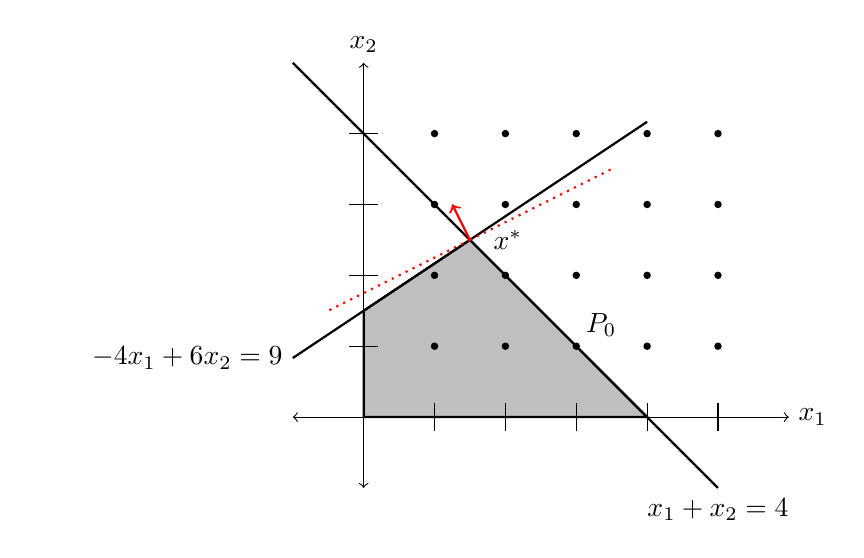
\begin{tikzpicture}[scale=0.90]
    \coordinate (a) at (0,0);
    \coordinate (b) at (4,0);

    \coordinate (c1x) at ( 5, -1);
    \coordinate (c1y) at (-1,  5);

    \coordinate (c2y) at (-1, 0.833333);
    \coordinate (c2x) at ( 4, 4.166666);

    \coordinate (c) at (intersection of c1x--c1y and c2x--c2y);

    \draw (c) node[right]{\, $x^*$};

    \coordinate (d) at (0,1.5);

    \draw[thick,fill=lightgray] (a) -- (b) -- (c) -- (d) --cycle;
    \draw[thick] (c1y) -- (c1x) node[below] {\BLACK{$x_1 + x_2 = 4 $}};  
    \draw[thick] (c2x) -- (c2y) node[left] {\BLACK{$\quad\quad -4x_1 + 6x_2 = 9  $}};
    \draw[thick,red,->] (c) -- +(-0.25,0.5);

    \draw[thick,dotted,red,-] (c) -- +(2,1);
    \draw[thick,dotted,red,-] (c) -- +(-2,-1);

    \draw[<->] (-1,0) -- (6,0) node[right] {$x_1$};
    \draw[<->] (0,-1) -- (0,5) node[above] {$x_2$};

    \foreach \i in {-0,...,5} {
        \draw (\i,-0.2) -- (\i,0.2); 
    }
    \foreach \i in {-0,...,4} {
        \draw (-0.2, \i) -- (0.2, \i);
    }

    \foreach \i in {1,...,5} {
       \foreach \j in {1,...,4} {
         \fill (\i,\j) circle (1.5pt);
       }
    }
    \draw (3,1) node[above right] {$P_0$};
  \end{tikzpicture}


  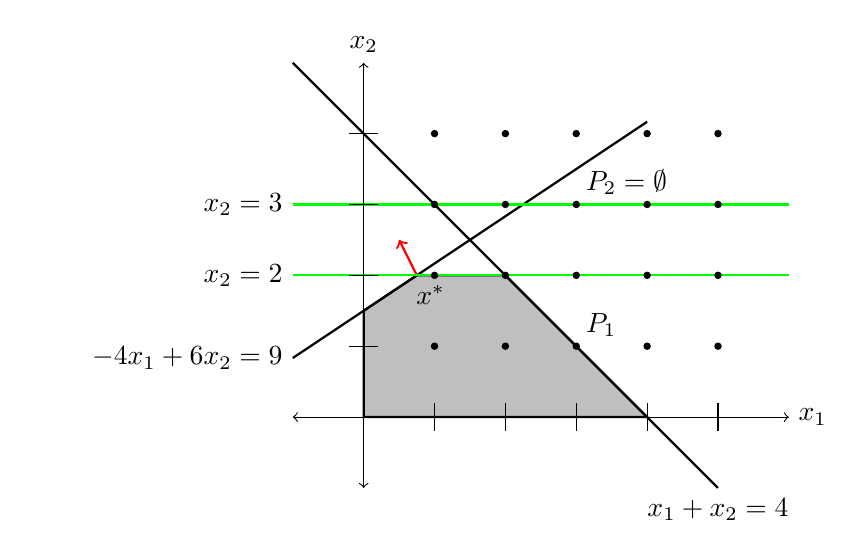
\begin{tikzpicture}[scale=0.90]
    \coordinate (a) at (0,0);
    \coordinate (b) at (4,0);

    \coordinate (c1x) at ( 5, -1);
    \coordinate (c1y) at (-1,  5);

    \coordinate (c2y) at (-1, 0.833333);
    \coordinate (c2x) at ( 4, 4.166666);

    \coordinate (c) at (intersection of c1x--c1y and c2x--c2y);

    \coordinate (d) at (0,1.5);

    \coordinate (e) at (2,2);
    \coordinate (f) at (0.75,2);

    \draw[thick,fill=lightgray] (a) -- (b) -- (e) -- (f) -- (d) --cycle;
    \draw[thick] (c1y) -- (c1x) node[below] {\BLACK{$x_1 + x_2 = 4 $}};  
    \draw[thick] (c2x) -- (c2y) node[left] {\BLACK{$\quad\quad -4x_1 + 6x_2 = 9  $}};
    \draw[thick,red,->] (f) -- +(-0.25,0.5);

    \draw (f) node[below]{\quad $x^*$};

    \draw[thick,green,-] (6,2) -- (-1,2) node[left] {\BLACK{$x_2 = 2$}};
    \draw[thick,green,-] (6,3) -- (-1,3) node[left] {\BLACK{$x_2 = 3$}};

    \draw[<->] (-1,0) -- (6,0) node[right] {$x_1$};
    \draw[<->] (0,-1) -- (0,5) node[above] {$x_2$};

    \foreach \i in {-0,...,5} {
        \draw (\i,-0.2) -- (\i,0.2); 
    }
    \foreach \i in {-0,...,4} {
        \draw (-0.2, \i) -- (0.2, \i);
    }

    \foreach \i in {1,...,5} {
       \foreach \j in {1,...,4} {
         \fill (\i,\j) circle (1.5pt);
       }
    }
    \draw (3,3) node[above right] {$P_2 = \emptyset$};
    \draw (3,1) node[above right] {$P_1$};
  \end{tikzpicture}


  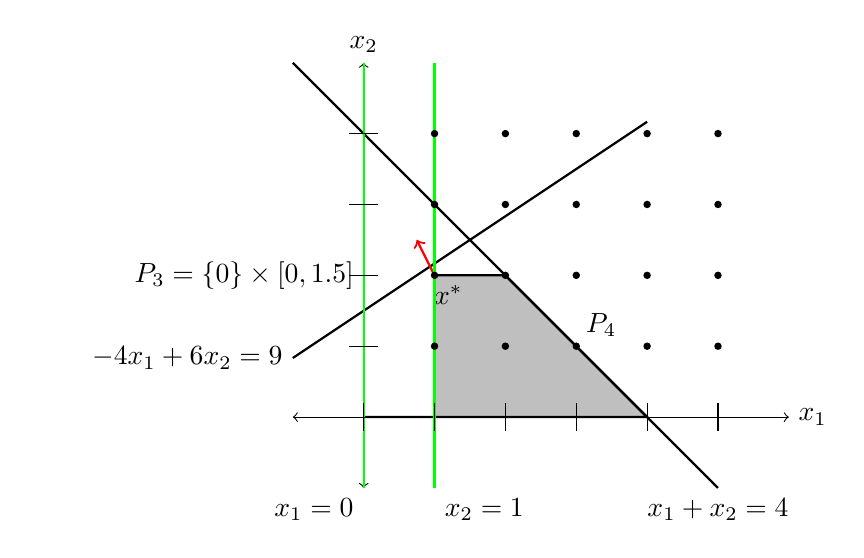
\begin{tikzpicture}[scale=0.90]
    \coordinate (a) at (0,0);
    \coordinate (b) at (4,0);

    \coordinate (c1x) at ( 5, -1);
    \coordinate (c1y) at (-1,  5);

    \coordinate (c2y) at (-1, 0.833333);
    \coordinate (c2x) at ( 4, 4.166666);

    \coordinate (c) at (intersection of c1x--c1y and c2x--c2y);

    \coordinate (d) at (0,1.5);

    \coordinate (e) at (2,2);
    \coordinate (f) at (0.75,2);

    \coordinate (g) at (1,2);
    \coordinate (h) at (1,0);

    \draw[thick,fill=lightgray] (a) -- (b) -- (e) -- (g) -- (h) --cycle;
    \draw[thick] (c1y) -- (c1x) node[below] {\BLACK{$x_1 + x_2 = 4 $}};  
    \draw[thick] (c2x) -- (c2y) node[left] {\BLACK{$\quad\quad -4x_1 + 6x_2 = 9  $}};
    \draw[thick,red,->] (g) -- +(-0.25,0.5);

    \draw (g) node[below]{\quad $x^*$};

    \draw[<->] (-1,0) -- (6,0) node[right] {$x_1$};
    \draw[<->] (0,-1) -- (0,5) node[above] {$x_2$};

    \draw[thick,green,-] (0,5) -- (0,-1) node[below left] {\BLACK{$x_1 = 0$}};
    \draw[thick,green,-] (1,5) -- (1,-1) node[below right] {\BLACK{$x_2 = 1$}};

    \foreach \i in {-0,...,5} {
        \draw (\i,-0.2) -- (\i,0.2); 
    }
    \foreach \i in {-0,...,4} {
        \draw (-0.2, \i) -- (0.2, \i);
    }

    \foreach \i in {1,...,5} {
       \foreach \j in {1,...,4} {
         \fill (\i,\j) circle (1.5pt);
       }
    }
    \draw (0,2) node[left] {$P_3 = \{0\} \times [0, 1.5]$};
    \draw (3,1) node[above right] {$P_4$};
  \end{tikzpicture}


\end{center}
\caption{\label{fig::ex_branch_bound}
A branch-and-bound example.}
\end{figure}





A branch-and-bound computation is often represented by a so-called 
{\hi branch-and-bound tree}.{\index{Branch-and-bound tree}} 
This is in fact rather an arborescence
than a tree. Its nodes are the polyhedra $P_j$ that are considered 
during the computation, and $P_0$ is the root. For any $P_j$, the 
nodes $P_{2j+1}$ and  $P_{2j+2}$ are its children (if they exist).



In line~\ref{bb::line_choose_pj} of the algorithm, we have to choose
the next LP to be solved, and in line~\ref{bb::line_choose_xi}
we have to decide which non-integral component is used for creating
new sub-problems.
There are different strategies for these
steps (branching rules).{\index{Branching rule}} 
For example, it is often reasonable to store
the elements of $\mathcal{K}$ in a last-in-first-out queue and to
choose the last element that has been added to $\mathcal{K}$. In the
branch-and-bound tree, this corresponds to a leaf with the biggest
distance to the root. This strategy can reduce the time until the first
feasible solution has been found. Another reasonable branching rule
consist in choosing a polyhedron $P_j$ for which
$\max\{c^tx \mid x \in P_j\}$ is as large as possible. Note that
the maximum over all these values for all $P_j \in \mathcal{K}$
gives an upper bound $U$ on the best possible solution that can
still be computed. Hence, by choosing a $P_j$ with 
$\max\{c^tx \mid x \in P_j\} =U$, we get a chance to reduce $U$.
This can be useful if we do not want to compute an exact optimum
solution but we stop as soon as $U - L$ is small enough.

For the choice of $x^*_i$ a common strategy is to choose $x^*_i$
such that $|x^*_i - \lfloor x^*_i \rfloor -  \frac{1}{2}|$ is minimized.
Another, more time-consuming approach is to choose $x^*_i$ such that
the effect on the objective function is maximized (strong branching).



{\bf Further remarks:}\vspace*{-0.3cm}
\begin{itemize}
\item In order to get at least a finite algorithm, we have to guarantee
      that in line~\ref{bb::subLP} we always find a integral optimum 
      solution if $P_j$ is integral.
\item Instead of initializing $L$ with $-\infty$, it is often possible
      to compute some reasonable integral solution by some heuristics.
      In particular this is often the case for combinatorial problems.
\item If one only wants to compute an approximative solution, the 
      condition $c^* > L$ can be strengthened to $c^* > L (1 + \epsilon)$.
      This way, some optimum solution may be cut off but the running
      can sometimes be reduced drastically. In many cases, an optimum
      solution is computed quite early but then much time is needed
      just in order to prove that the solution is optimum. 
\item The branch-and-bound strategy can be combined with a cutting-plane
      algorithm (see the previous section). For each sub-polyhedron $P_j$,
      one can try to find 
      hyperplanes separating some non-integral vectors in $P_j$ from
      $(P_j)_I$. This combination is called
      {\hi branch-and-cut method}.{\index{Branch-and-cut method}}
      For example, this approach has been used for solving quite large
      Traveling Salesman Problems (see \cite{PadR91}).
\end{itemize}

% \begin{tikzpicture}[xscale=3.0,yscale=4.0,domain=1.000:3.500,samples=120]
%     \draw[->] (0.9,1) -- (4,1) node[below] {$\gamma$};
%     \draw[->] (1,0.9) -- (1,2.2) node[left] {};
%     \foreach \i in {1,2,...,3} {
%         \draw (\i,1.) -- (\i,0.9) node[below] {$\i$};
%     }
% %    \foreach \i in {1.0,1.5,...,2.0} {
% %        \draw (1.1,\i) -- (0.9,\i) node[left] {$\i$};
% %    }
%     \draw (1.1,1.0) -- (0.9,1.0) node[left] {$1.0$};
%     \draw (1.1,1.2) -- (0.9,1.2) node[left] {$1.2$};
%     \draw (1.1,1.4) -- (0.9,1.4) node[left] {$1.4$};
%     \draw (1.1,1.6) -- (0.9,1.6) node[left] {$1.6$};
%     \draw (1.1,1.8) -- (0.9,1.8) node[left] {$1.8$};
%     \draw (1.1,2.0) -- (0.9,2.0) node[left] {$2.0$};

%     \draw[dotted] (1.707,2.2) -- (1.707,0.8) node[below] {$\gamma_0 = \frac{2 + \sqrt{2}}{2} \approx 1.707$};
    
    
% %    \draw[blue] plot (\x,{max(40-0.2*\x},2/\x));
%      \draw[red] plot (\x,{max(2/\x, (4*\x)/(4*\x - 1)) }) node[above] {$\max\left\{\frac{4\gamma}{4\gamma-1}, \frac{2}{\gamma} \right\}$};
%      \draw[red,dotted] plot (\x,{2/\x });% node[above] {$\frac{4\gamma}{4\gamma-1}$};
%      \draw[red,dotted] plot (\x, {(4*\x)/(4*\x - 1) });
% \end{tikzpicture}



\printindex



%\ifdefined\OnlineVersion{}\else


\bibliographystyle{myalpha}
\bibliography{lgo}
\end{document}
\iffalse

Further topics:

Lagrange relaxation: Kurzversionen z.B. im Skript von Stephan von 2017
oder beim Buch von Schijver.

\cite{Len83}: ILP with fixed number of variables can be solved in polynomial time.
(see also the chapter in \cite{Sch86}, the lecture notes used in the seminar and 
\cite{Eis03} who cites some improvements to Lenstra, too).

% E-Mail vom 30.7.2021:
%A more general comment, I think it would be nice if the borrowed terminology 
%(the ones concerning graphs especially the boundaries as delta +- )from the 
%algorithmic mathematics course could be rephrased. I personally had to dig 
%through the other course book to figure them out. Same was the case with some 
%less common terminology such as regular for invertible matrices. 





\fi % iffalse

\ifdefined\OnlineVersion{}\else

\fi % onlineversion

\newpage

\selectlanguage{english}

\iffalse
%%%%%%%%%%%%%%%%%%%%%%%%%%%%%%%%%%%%%%%%%%%%%%%%%
%\newcommand{\bib}[3]{\bibitem[\protect\citeauthoryear{#1}{#2}]{#3}} 
\renewcommand{\refname}{Bibliography}
\begin{thebibliography}{XXXX}
%%%%%%%%%%%%%%%%%%%%%%%%%%%%%%%%%%%%%%%%%%%%%%%%%


\small

\selectlanguage{german}

\bib{Adler, Karp, and Shamir}{1987}{AdlKS87}
Adler, I., Karp, R.M., Shamir, R. [1987]:
{\it A simplex variant solving an $m \times d$ linear program
in $O(\min(m^2,d^2))$ expected number of steps.}
Journal of Complexity,
3, 372--387, 1987.

\bib{Ahuja, Magnanti, and Orlin}{1993}{AhuMO93}
Ahuja, R.K., Magnanti, T.L., and Orlin [1993]:
{\it Network Flows: Theory, Algorithms, and Applications.}
Prentice Hall, 1993.

\bib{Anthony and Harvey}{2012}{AntH12}
Anthony, M., and Harvey, M. [2012]:
{\it Linear Algebra: Concepts and Methods.}
Cambridge University Press, 2012.

\bib{B\'{a}r\'{a}ny, Howe, and Lov\'{a}sz}{1992}{BarHL92}
B\'{a}r\'{a}ny, I., Howe, R., and Lov\'{a}sz, L. [1992]:
{\it On integer points in polyhedra: a lower bound.}
Combinatorica, 12, 135--142, 1992.

\bib{Bertsimas and Tsitiklis}{1997}{BerT97}
Bertsimas, D., and Tsitsiklis, J.N. [1997]:
{\it Introduction to Linear Optimization.}
Athena Scientific, 1997.

\bib{Bertsimas and Weismantel}{2005}{BerW05}
Bertsimas, D., and Weismantel, R. [2005]:
{\it Optimization over Integers.}
Dynamic Ideas, 2005.

\bib{Bland}{1977}{Bla77}
Bland, R.G. [1977]: 
{\it New finite pivoting rules for the simplex method.}
Mathematics of Operations Research, 2, 103--107, 1977.

\bib{Borgwardt}{1982}{Bor82}
Borgwardt, K. [1982]:
{\it The average number of pivot steps required by the simplex method
is polynomial.}
Zeitschrift f"ur Operations Research, 26, 157--177, 1982.

\bib{Bosch}{2007}{Bos07}
Bosch, S. [2007]:
{\it Lineare Algebra.}
4th edition, Springer, 2007.

\bib{Chv\'{a}tal}{1983}{Chv83}
Chv\'{a}tal, V. [1983]:
{\it Linear programming.}
Series of books in the mathematical sciences, W.H. Freeman, 1983.

\bib{Cohn}{1980}{Coh80}
Cohn, D.L. [1980]:
{\it Measure Theory.}
Birkh"auser, 1980.

\bib{Cunningham}{1976}{Cun76}
Cunningham, W.H. [1976]:
{\it A network simplex method.}
Mathematical Programming, 11, 105--116, 1976.

\bib{Dadush and Hulberts}{2019}{DadH19}
Dadush, D. and Hulberts, S. [2019]:
{\it A Friendly Smoothed Analysis of the Simplex Method.}
SIAM Jounal on Computing, 49, 5, 449--499, 2019

\bib{Dantzig}{1951}{Dan51}
Dantzig, G.B. [1951]:
{\it Maximization of a linear function of variables subject to linear
inequalities.}
In: Koopmans, T.C (ed.), Activity Analysis of Production and Allocation,
359--373, Wiley, 1951.

\bib{Dunkel and Schulz}{2013}{DunS13}
Dunkel, J. and Schulz, A.S. [2013]:
{\it The Gomory-Chv\'{a}tal closure of a non-rational polytope is a rational polytope.}
Mathematics of Operation Research, 38, 1, 63--91, 2013.

\bib{Edmonds}{1965}{Edm65}
Edmonds, J. [1965]:
{\it Maximum matching and polyhedron with (0,1) vertices.}
Journal of Research of the National Bureau of Standards, B, 69, 125--130,
1965.

\bib{Eisenbrand}{2003}{Eis03}
Eisenbrand, F. [2003]:
{\it Fast integer programming in fixed dimension.}
Lecture Notes in Computer Science, 2832, 196--207, 2003.

\bib{Fischer}{2009}{Fis09}
Fischer, G. [2009]:
{\it Lineare Algebra: Eine Einf"uhrung f"ur Studienanf"anger.}
18th edition, Springer, 2013.

\bib{Ghouila-Houri}{1962}{Gho62}
Ghouila-Houri, A. [1962]:
{\it
Charact\'{e}risation des matrices totalement unimodulaires.}
Comptes Rendus Hebdomadaires des S\'{e}ances de l'Acad\'{e}mie des
Sciences (Paris), 254, 1192-1194, 1962.

\bib{Giles and Pulleyblank}{1979}{GilP79}
Giles, F.R. and Pulleyblank, W.R. [1979]:
{\it
Total dual integrality and integer polyhedra.}
Linear Algebra and Its Applications, 25, 191--196, 1979.

\bib{Goldfarb and Sit}{1979}{GolS79}
Goldfarb, D. and Sit, W.Y. [1979]:
{\it Worst case behavior of the steepest edge simplex method.}
Discrete Applied Mathematics, 1, 4, 277--285, 1979.

\bib{Gomory}{1963}{Gom63}
Gomory, R.E. [1963]:
{\it An algorithm for integer solutions of linear programs.}
In: Recent Advances in Mathematical Programing (R.L.\ Graves, P.\ Wolfe, eds.),
McGraw-Hill, 269--302, 1963.

\bib{Gr\"otschel, Lov\'{a}sz, and Schrijver}{1981}{GorLS81}
Gr\"otschel, M., Lov\'{a}sz, L. and Schrijver, A. [1981]:
{\it The ellipsoid method and its consequences in combinatorial optimization.}
Combinatorica, 1, 169--197, 1981.

\bib{Guenin, K\"onemann, and Tun\c{c}el}{2014}{GueKT14}
Guenin, B., K\"onemann, J., and Tun\c{c}el, L. [2014]:
{\it A Gentle Introduction to Optimization.}
Cambridge University Press, 2014.

\bib{Hoffman and Kruskal}{1956}{HofK56}
Hoffman, A. and Kruskal, J. [1956]:
{\it
Integral boundary points of convex polyhedra.
}
Linear Inequalities and Related Systems (H.\ Kuhn, A.\ Tucker, eds.),
Annals of Mathematics Studies, 38, 223--246, 1956.

\bib{Hougardy and Vygen}{2018}{HouV18}
Hougardy, S., and Vygen, J. [2018]:
{\it Algorithmische Mathematik.}
Second edition, Springer, 2018.

%\bib{Hu and Kahng}{2016}{HuK16}
%Hu, T.C. and Kahng, A.B. [2016]:
%{\it
%Linear and Integer Programming Made Easy.}
%Springer, 2016.

\bib{Kafer}{2022}{Kaf22}
Kafer, S. [2022]:
{\it
Polyhedral Diameters and Applications to Optimization.}
PhD Thesis, University of Waterloo, 2022.

\bib{Kalai and Kleitman}{1992}{KalK92}
Kalai, G., and Kleitman, D. [1992]:
{\it 
A quasi-polynomial bound for the diameter of graphs of polyhedra.}
Bulletin of the American Mathematical Society, 26, 315--316, 1992.

\bib{Karmakar}{1984}{Kar84}
Karmakar, L. [1984]:
{\it A new polynomial-time algorithm for linear programming.}
Combinatorica, 4, 373--395, 1984.

\bib{Karloff}{1991}{Kar91}
Karloff, H. [1991]:
{\it Linear Programming.}
Birkh\"{a}user, 1991.

\bib{Khachiyan}{1979}{Kha79}
Khachiyan, L. [1979]:
{\it A polynomial algorithm for linear programming.}
Soviet Mathematics Doklady, 20, 191--194, 1979.

\bib{Klee and Minty}{1972}{KleM72}
Klee, V., and Minty, G.J. [1972]:
{\it How good is the simplex algorithm?}
In: Inequalities III (O. Shisha, ed.), Academic Press,
159--175, 1972.

\bib{Korte and Vygen}{2018}{KorV18}
Korte, B., and Vygen, J. [2018]:
{\it Combinatorial Optimization: Theory and Algorithms.}
Sixth edition, Springer, 2018.

\bib{Lang}{1987}{Lan87}
Lang, S. [1987]:
{\it Linear Algebra.}
Third edition, Springer, 1987.

\bib{Lee, Sidford, and Wong}{2015}{LeeSW15}
Lee, T., Sidford, A., Wong, S.C. [2015]:
{\it 
A Faster Cutting Plane Method and its
Implications for Combinatorial and Convex Optimization.}
arxiv.org/abs/1508.04874,
Symposium on Foundations of Computer Science, 2015.

\bib{Lenstra}{1983}{Len83}
Lenstra, H.W. [1983]:
{\it
Integer programming with a fixed number of variables.}
Mathematics of Operations Research, 8, 538--548, 1983.

\bib{Matou\v{s}ek and G"artner}{2007}{MatG07}
Matou\v{s}ek, J., and G"artner, B. [2007]:
{\it Understanding and Using Linear Programming.}
Springer, 2007.

\bib{Megiddo}{1984}{Meg84}
Megiddo, N. [1984]:
{\it Linear programming in linear time when the dimension is fixed.}
Journal  of the ACM, 31, 114--127, 1984.

\bib{Mehlhorn and Saxena}{2015}{MehS15}
Mehlhorn, K.,  and Saxena, S. [2015]:
{\it A still simpler way of introducing the interior-point method for linear
   programming.}
%http://arxiv.org/abs/1510.03339, 2015.
Computer Science Review, 22, 1--11, 2016.

\bib{Padberg}{1999}{Pad99}
Padberg, M. [1999]:
{\it Linear Optimization and Extensions.}
Second edition, Springer, 1999

\bib{Padberg and Rao}{1982}{PadR82}
Padberg, M., and Rao, M. [1982]:
{\it Odd minimum cut-sets and $b$-matchings.}
Mathematics of Operations Research, 7, 67--80, 1982.

\bib{Padberg and Rinaldi}{1991}{PadR91}
Padberg, M., and Rinaldi, G. [1991]:
{\it A Branch-and-Cut Algorithm for the Resolution of Large-Scale 
Symmetric Traveling Salesman Problems.}
SIAM Review, 33, 1, 60--100, 1991.

\bib{Pan}{2014}{Pan14}
Pan, P.-Q. [2014]:
{\it Linear Programming Computation.}
Springer, 2014.

\bib{Panik}{1996}{Pan96}
Panik, M.J. [1996]:
{\it Linear Programming: Mathematics, Theory and Algorithms.}
Kluwer Academic Publishers, 1996.

\bib{Roos, Terlaky, and Vial}{2005}{RooTV05}
Roos, C., Terlaky, T., Vial, J.-P. [2005]:
{\it Interior Point Methods for Linear Optimization.}
Second edition, Springer, 2005.

\bib{Rubin}{1970}{Rub70}
Rubin, D. [1970]:
{\it On the unlimited number of faces in integer hulls of
linear programs with a single constraint.}
Operations Research,
18, 5, 940 -- 946, 1970.

\bib{Saigal}{1995}{Sai95}
Saigal, R. [1995]:
{\it Linear Programming. A Modern Integrated Analysis.}
Springer, 1995.

\bib{Santos}{2011}{San11}
Santos, F. [2011]:
{\it A counterexample to the Hirsch conjecture.}
Annals of Mathematics, 176, 1, 383--412, 2011.

\bib{Schrijver}{1980}{Sch80}
Schrijver, A. [1980]:
{\it On cutting planes.}
Annals of Discrete Mathematics, 9, 291--296, 1980.

\bib{Schrijver}{1986}{Sch86}
Schrijver, A. [1986]:
{\it Theory of Linear and Integer Programming.}
Wiley, 1986.

\bib{Sierksma and Zwols}{2015}{SieZ15}
Sierksma, G., and Zwols, Y. [2015]:
{\it Linear and Integer Optimization. Theory and Practice.}
Third edition, CRC Press, 2015.

\bib{Spielmann and Teng}{2005}{SpiT05}
Spielmann, D.A., and Teng, S.-H. [2005]:
{\it Smoothed analysis of algorithms:
Why the simplex algorithm usually takes polynomial time.}
Journal of the ACM, 51, 3, 385 -- 463, 2004.

\bib{Strang}{1980}{Str80}
Strang, G. [1980]:
{\it Linear Algebra and Its Applications.}
Second edition, Academic Press, 1980.

\bib{Tardos}{1986}{Tar86}
Tardos, \'{E}. [1986]:
{\it A strongly polynomial algorithm to solve combinatorial linear programs.}
Operations Research,
34, 2, 250 -- 256, 1986.

\bib{Terlaky}{2001}{Ter01}
Terlaky, R.J. [2001]:
{\it An easy way to teach interior point methods.}
European Journal of Operational Research, 130, 1--19, 2001.

\bib{Todd}{2014}{Tod14}
Todd, M. [2014]:
{\it An improved Kalai-Kleitman bound for the Diameter of a polyhedron.}
SIAM Jounal on Discrete Mathematics, 28, 4, 1944--1947, 2014.

\bib{Vanderbei}{2014}{Van14}
Vanderbei, R.J. [2014]:
{\it Linear Programming: Foundations and Extensions.}
Fourth edition, Springer, 2014.

\bib{Wright}{1997}{Wri97}
Wright, S.J. [1997]:
{\it Primal-Dual Interior-Point Methods.}
SIAM, 1997.

\bib{Ye}{1992}{Ye92}
Ye, Y. [1992]:
{\it On the finite convergence of interior-point algorithms
for linear programming.}
Mathematical Programming, 57, 325--335, 1992.


\bib{Ye}{1997}{Ye97}
Ye, Y. [1997]:
{\it Interior Point Algorithms. Theory and Analysis.}
Wiley, 1997.


\bib{Ziegler}{2007}{Zie07}
Ziegler, G. [2007]:
{\it Lectures on Polytopes.}
Seventh Printing, Springer, 2007.

%%%%%%%%%%%%%%%%%%%%%%%%%%%%%%%%%%%%%%%%%%%%%%%%%
\end{thebibliography}
%%%%%%%%%%%%%%%%%%%%%%%%%%%%%%%%%%%%%%%%%%%%%%%%%
\fi
%\ifdefined\OnlineVersion{}\else

\printindex

%\fi % not OnlineVersion

\end{document}





